%
% PROJECT: <ETD> Electronic Thesis and Dissertation Initiative
%   TITLE: LaTeX report template for ETDs in LaTeX
%  AUTHOR: Neill Kipp, nkipp@vt.edu
%     URL: http://etd.vt.edu/latex/
% SAVE AS: etd.tex
% REVISED: September 6, 1997 [GMc 8/30/10]
% 

% Instructions: Remove the data from this document and replace it with your own,
% keeping the style and formatting information intact.  More instructions
% appear on the Web site listed above.

%\documentclass[12pt,dvips]{report}
\documentclass[12pt]{report}
\usepackage{bm}
\usepackage{amsmath}
\newenvironment{MyFigure}[1][]{\begin{figure}[#1]\vspace{1.0cm}}{\vspace{1.0cm}\end{figure}}
%\usepackage[dvips]{graphicx}
%\usepackage{graphicx}
\newcommand{\overbar}[1]{\mkern 2.2mu\overline{\mkern-2.2mu#1\mkern-2.2mu}\mkern 2.2mu}

%\usepackage{tocloft}
%\renewcommand\cftchapfont{\fontsize{11pt}}
%\renewcommand\cftsecfont{\fontsize{11pt}}
%\renewcommand\cftsubsecfont{\fontsize{11pt}}
%\renewcommand\cftsubsubsecfont{\fontsize{11pt}}
%
%\renewcommand\cftchappagefont{\fontsize{11pt}}
%\renewcommand\cftsecpagefont{\fontsize{11pt}}
%\renewcommand\cftsubsecpagefont{\fontsize{11pt}}
%\renewcommand\cftsubsubsecpagefont{\fontsize{11pt}}

\setlength{\textwidth}{6.5in}
\setlength{\textheight}{8.5in}
\setlength{\evensidemargin}{0in}
\setlength{\oddsidemargin}{0in}
\setlength{\topmargin}{0in}

\setlength{\parindent}{0pt}
\setlength{\parskip}{0.1in}

\setcounter{secnumdepth}{3}
\setcounter{tocdepth}{3}

% Uncomment for double-spaced document.
\renewcommand{\baselinestretch}{2}

\usepackage{epsf}

\usepackage[final]{graphicx}
\usepackage{subcaption}

\begin{document}

\thispagestyle{empty}
\pagenumbering{roman}
\begin{center}

% TITLE
{\Large 
Towards a Reduced-Scaling Method for Calculating Coupled Cluster Response Properties
}

\vfill

Ashutosh Kumar

\vfill

Dissertation submitted to the Faculty of the \\
Virginia Polytechnic Institute and State University \\
in partial fulfillment of the requirements for the degree of

\vfill

Doctor of Philosophy \\
in \\
Chemistry

\vfill

T. Daniel Crawford, Chair \\
Eduard Valeyev \\
Diego Troya \\
Alan Esker

\vfill

May 9, 2018 \\
Blacksburg, Virginia

\vfill

Keywords: Coupled Cluster, Reduced-Scaling, Response Properties
\\
Copyright 2018, Ashutosh Kumar

\end{center}

\pagebreak

\thispagestyle{empty}
\begin{center}

{\Large
Towards a Reduced-Scaling Method For Calculating Coupled Cluster Response Properties 
}\\
%\vfill

\vspace{8em}
Ashutosh Kumar
\vspace{8em}

%\vfill

(ABSTRACT)

%\vfill

\end{center}
One of the central problems limiting the application of accurate {\em ab
initio} methods to large molecular systems is their high computational costs,
i.e., their computing and storage requirements exhibit polynomial scaling with
the size of the system. For example, the coupled cluster singles and doubles 
method with the perturbative inclusion of triples: the CCSD(T) model, 
which is considered as the ``gold standard'' of quantum chemistry scales as 
${\cal O}(N^7)$ in its canonical formulation, where $N$ is a measure of the 
system size. However, the steep scaling associated with these methods is 
unphysical since the property of dynamic electron correlation or dispersion 
(for insulators) is local in nature and decay as $R^{-6}$ power of distance. 
Different reduced-scaling techniques which attempt to exploit this inherent 
sparsity in the wavefunction have been used in conjunction with the coupled cluster 
theory to calculate ground-state properties of molecular systems with
hundreds of heavy atoms in reasonable computational time. However, efforts towards
extension of these methods for describing response properties which are related to the 
derivative of the wavefunction with respect to external electric or/and magnetic fields, 
like polarizabilities, optical rotations, etc., have been fairly limited and conventional 
reduced-scaling algorithms have been shown to yield large and often erratic deviations from 
the full canonical results for these properties. In this work, we identify the reasons behind 
the unsatisfactory performance of the pair natural orbital (PNO) based reduced-scaling 
approach for calculating linear response properties at the coupled cluster level of theory 
and propose novel modifications, which we refer to as PNO++, (A. Kumar and T. D. Crawford, 
2018, {\em manuscript in preparation}) that can provide the necessary accuracy at significantly 
lower computational costs. The motivation behind the PNO++ approach comes from our works 
on the (frozen) virtual natural orbitals (FVNO), which can be seen as a precursor to the concept 
of PNOs (A. Kumar and T. D. Crawford, {\em J. Phys. Chem. A}, 2017, {\bf 121(3)}, pp 708-716) and 
the improved FVNO++ method (A. Kumar and T. D. Crawford, 2018, {\em manuscript in 
preparation}). The essence of these modified schemes (FVNO++ and PNO++) lie in finding suitable 
field perturbed one electron densities to construct ``perturbation aware" virtual spaces which,
by construction, are much more compact for calculating response properties, making them ideal
for applications to large molecular systems. \\\\
%The virtual natural orbitals
%In this work, we identify some of the reasons behind  the failure of popular local correlation models like Frozen Virtual Natural Orbitals (FVNO) 
%and Pair Natural Orbitals (PNO) in capturing the response of the wavefunction. 
%Consequently, we introduce  novel modifications to these schemes which we call FVNO++ 
%and PNO++ respectively. Initial results indicate that these techniques 
%significantly outperform their conventional counterparts and can be used for 
%calculating response properties of large molecular systems.
\vfill
% GRANT INFORMATION
This work was supported by a grant (CHE-1465149) from
the U.S. National Science Foundation. Advanced Research Computing 
Center at Virginia Tech provided the necessary computational resources and technical 
support for all the calculations reported here.

\pagebreak

% Dedication and Acknowledgments are both optional
% \chapter*{Dedication}
%\chapter*{Acknowledgments}

\tableofcontents
\pagebreak

\listoffigures
\pagebreak

\listoftables
\pagebreak

\pagenumbering{arabic}
\pagestyle{myheadings}

\def\ket#1{| #1 \rangle}
\def\bra#1{\langle #1 |}
\def\bm#1{\mbox{\boldmath $#1$}}
\def\degrees{deg dm$^{-1}$ (g/mL)$^{-1}$}
\def\optrot{$[\alpha]$}
\def\crt#1{a_{#1}^{\dagger}}
\def\ann#1{a_{#1}^{\ }}
\def\cgs{($10^{-40}$ cgs)}


\chapter{Introduction}
\markright{Ashutosh Kumar \hfill Chapter 1. Introduction \hfill}
%\section{Introduction}

%    a. chirality - same story as my Internal Seminar.
%    b. Drug thalidomide example
%    c. Chiroptical spectroscopy
%    d. Theory as a tool!
%    e. Some history of OR calculations (Harley's thesis)
%    f. TD-DFT not enough in most cases, CC needed (known problems of DFT)
%    g. Challenges of CC - (mention about MD as well.)
%    h. My work comes in here!
%	i. local correlatin - which chapter discusses what... end by conclusion..
\section{Chirality}
Lord Kelvin was the first person to use the word `chiral' in his lecture 
at Oxford University in 1894: ``I call any geometrical figure, or group of points, 
`chiral', and say that it has chirality if its image in a plane mirror, ideally realized, 
cannot be brought to coincide with itself"\cite{Kelvin}. 
\\
There are different ways in which a molecule 
could be chiral. The most common example being the presence of a chiral center 
like a carbon or nitrogen atom with four different substituents. Axial chirality, usually 
possessed by molecules with cumulated double bonds like allenes and chirality planes 
found in compounds like paracyclophanes are some other popular examples. \\
A chiral molecule and its mirror image are known as enantiomers. Although the
enantiomers have idential physical properties like boiling and melting points, their
interactions with a chiral environment can be quite different. For example,
while the (R) enantiomer of the compound limonene smells like lemons and oranges, the (S) 
enantiomer on the other hand smells like turpentine. Thus, the interaction of the (S) enantiomer 
with the chiral molecules constituting the olfactory receptors responsible for the sensation of smell 
is totally different from its fellow enantiomer. The enantiomers also interact differently with 
the left- and right-hand circularly polarized (LCP and RCP) light in processes of absorption, 
refraction, etc. A chiral molecule posesses the properties of circular dichroism (CD) and 
circular birefringence, i.e. it has different absorption coefficents and refractive indices 
for the LCP and RCP light respectively. As a result of circular birefringence, the plane of 
polarization of a plane-polarized light in a chiral medium gets rotated/shifted by an amount known as 
the optical rotation of the medium. An enantiomeric pair of chiral molecules has equal magnitudes of 
optical rotation but in opposite directions.\\
Since almost every part of the human body is composed of chiral molecules, its unsurprising that
more than 60\% of the pharmaceutical drugs are chiral as well. One of the most 
important aspect of the drug-design research is to be able to define the absolute configuration 
(AC) of these drug molecules in order to study their behaviour in biological systems as 
many biological activities are only associated with one specific AC. A very tragic example
in this regard is that of the drug thalidomide, which was originally prescribed to pregnant women in 
Europe in 1950s to cure morning sickness but resulted in birth-defects in thousands of 
infants. It was found through a study done on rodents that the (R) enantiomer of thalidomide is indeed 
a sedative but the (S) enantiomer is a teratogen\cite{Crawford06}. Furthemore, these enantiomers were 
found to rapidly interconvert in vivo in humans because of which separating 
these two forms before use doesn't help at all.
\\
The first step in experimental determination of AC either involves the separation of 
a racemic mixture (equal concentrations of both the enantiomers) into individual enantiomers
using chiral resolution methods like chiral column chromatography or a selective synthesis
of a given enantiomer using the process of asymmetric synthesis. X-ray crystallography would then be the 
most popular procedure to determine AC directly, provided one can crystallize the molecule first, which usually 
requires the presence of heavy atom(s). Alternatively, one can measure the distinct responses of 
the enantiomers in absorption using chiroptical spectroscopic techniques like electronic and vibrational 
CD (ECD and VCD) or can measure the optical rotation of the chiral compounds in both liquid 
and gas phase using regular and cavity ring-down polarimetry techniques\cite{Muller00} respectively.
These measurement are usually followed by a comparison against some suitable reference chiral
substrate. In this regard, accurate {\em ab initio} methods can help validate these experimental measurements.
%However, in cases of ambiguities regarding appropriate references, accurate {\em ab initio} methods can come to the rescue and 
%help validate these experimental measurements. 
Furthermore, designing an asymmteric synthesis might not be straightforward for many chiral systems, 
especially for the ones with large number of stereocenters. In such cases, theory can even take the 
lead and predict the corresponding AC. In other words, theoretical calculations of these chiroptical 
properties could serve as a very useful computational tool for modern organic chemists. In particular, 
accurate optical rotation calculations are highly desired as the experimental techniques for measuring 
this property are fairly stable and robust in both gas and liquid phases.
\\
%Theoretical and computational chemistry has grown by leaps and bounds over the
%past several decades. {\em ab initio} quantum chemical methods can now accurately
%predict a variety of molecular properties. More recently, these methods have
%been extended to calculate chiroptical
%properties like optical rotation. Theoretical calculations of optical rotation
%can be very useful in solving experimental chemical problems.  Specifically, they
%can provide a computational tool to modern organic chemists to determine
%the absolute stereochemical configuration of a chiral compound, thus alleviating the experimental difficulties
%involved.\\ 
\section{{\em Ab Initio} Optical Rotation Calculations}
Rosenfeld developed a quantum mechanical recipe for calculating optical rotations in the year
1929\cite{Rosenfeld29}. He showed that in the presence of an external electromagnetic field,
the induced dipole moment in a molecule can be written as:
\begin{equation}\langle\vec{\mu}\rangle = \bm{\alpha}\vec{E} + \frac{1}{\omega}\textbf{G}^\prime\frac{\partial\vec{B}}{\partial t}
\end{equation} where $\vec{E} $ and $\vec{B}$ are the time dependent electric and
magnetic field vectors respectively, $\omega$ is the frequency of the field, $\alpha$ is the electric dipole
polarizability tensor and the $\textbf{G}^\prime$ tensor, also known as the Rosenfeld tensor is associated 
with the property of optical rotation. Invoking the time-dependent Schr\"odinger's equation in conjunction 
with perturbation theory, expanding the expectation value of the electric dipole operator in orders of perturbation 
and identifying the term linear in $\vec{E}$ and $\frac{\partial\vec{B}}{\partial t}$, 
for exact states, the $\bm{\alpha}$ and $\textbf{G}^\prime$ tensors look like,
\\
\begin{equation}
\begin{split}
& \bm{\alpha}(\omega) = -\frac{2}{\hbar} \sum_{n \neq 0}\frac{\omega_{no}\bra
{\psi_o}\vec{\mu}\ket{\psi_n}\bra{\psi_n}\vec{\mu}\ket{\psi_o}}{{\omega_{no}}^2 - {\omega}^2 }\\
& \textbf{G}^{\prime}(\omega) = -\frac{2}{\hbar} \text{Im}\sum_{n \neq 0}\frac{\omega \bra
{\psi_o}\vec{\mu}\ket{\psi_n}\bra{\psi_n}\vec{m}\ket{\psi_o}}{{\omega_{no}}^2 - {\omega}^2 }.\\
\end{split}
\end{equation}
\\
Here, $\vec{\mu}$ and $\vec{m}$ are electric and magnetic dipole operators, 
$\vec{\mu} = \sum\limits_i q_i \vec{{r}_i}$ and $\vec{m} = \sum\limits_i \frac{q_i}{2m_i} \vec{{r}_i} \times \vec{{p}_i}$, $\omega$ is the frequency of light, $\omega_{no}$ is the excitation energy of the state $\psi_n$.
%\cite{CrawfordTamJPA07}. 
Im means the imaginary part of the equation and the summation runs over all the excited
states $\psi_n$. Specific rotation, ${\lbrack\alpha\rbrack}_\omega$ is related to the trace of the Rosenfeld tensor 
normalized by pathlength and concentration and is usually reported in the units of deg dm$^{\text{-1}}$(g/mL)$^{\text{-1}}$,\cite{Crawford06}
\\
\begin{equation}
{\lbrack\alpha\rbrack}_{\omega} = \frac{(72.0 \times 10^6){\hbar}^2 N_A\;\omega}{c^2{m_e}^2 M} \times \left[ \frac{1}{3}Tr(\textbf{G}^\prime)\right]
\end{equation}
\\
Here, $\textbf{G}^\prime$ and $\omega$ are in atomic units, c is the speed of light (m/s), m$_{\text{e}}$ is the 
mass of electron (kg), M is the molecular mass (amu) and $N_A$ is Avogadro's number. Calculating the 
$\textbf{G}^\prime$ tensor using equation (1.2) requires explicit calculations of a large number of 
excited states which is of course computationally prohibitive. A more practical approach is to invoke the response formalism
\cite{Kobayashi94,Koch90}, which casts these tensors as response functions,
\begin{equation}
\begin{split}
&\bm{\alpha}(\omega) = -\langle\langle\vec{\mu};\vec{\mu}\rangle\rangle\\
&\textbf{G}^{\prime}(\omega) = \text{Im}\langle\langle\vec{\mu};\vec{m}\rangle\rangle.\\
\end{split}
\end{equation} 
The response theory focuses on the perturbation of the ground state wavefunction in the presence of an external 
field, avoiding explicit calculations of excited states. Polavarapu was the first to use this theory to calculate 
{\em ab initio} specific rotations using the time dependent Hartree Fock (TDHF) method \cite{Polavarapu96}. 
The signs of the calculated values matched with that of the experiment for most of his structures, while their magnitudes 
differed generally by a factor of two. Inspired by Polavarapu's work, Cheeseman et al. \cite{Cheeseman00,Stephens01} 
included correlation effects in these calculations by using TD-DFT theory\cite{Runge84}. Using large basis sets with diffuse functions like 
aug-cc-pVDZ and aug-cc-pVTZ,\cite{Dunning89,Kendall92,Woon94} they were able to match the experimental values very closely, with a 
deviation of 20-25 degrees for a set of 28 chiral molecules. Ruud {\em et al.} extended the calculations to the coupled cluster (CC) level 
using CC response theory developed by Koch and J{\o}rgensen\cite{Koch90}, and obtained very 
promising results\cite{Ruud03}. Unsurprisingly, these simulations have been used to determine the AC of a large number of 
chiral molecules over the years\cite{Kondru99}. Specifically, the CC response theory has gained a reputation as  
a reliable theoretical recipe for accurate calculations of these properties. However, for a truly robust and reliable description of these response 
properties, one needs to take into account, a number of challenges associated with such simulations.
%However, all these calculations were done on single isolated molecules and thus, ideally, they should only be 
%expected to match vapor phase optical rotation (OR) values. 
\subsection{Challenges}
%Due to the non-variational nature of the coupled cluster theory, the specific rotation values calculated
%using the coupled cluster response theory suffer from problems of origin and gauge invariance. For example,
%using the length gauge representation of the electric dipole operator, 
%One of the major challenges faced by the coupled cluster respone theory is that of gauge and origin invariance.
%The origin dependence while using length-gauge representation is a consequence of the non-variational nature of the 
%coupled cluster wavefunction. Unlike HF and DFT methods, properties such as optical rotation computed via CCLR 
%are not origin independent even at the complete basis set limit, and the dependence cannot be resolved using GIAOs.6 
%The modified velocity gauge formalism for the electric dipole operator has been developed to help address this 
%issue. The velocity-gauge formalism, ⟨⟨⃗p, L⃗ ⟩⟩ω , allows for the trace of the property tensor to be origin 
%invariant. Here ⃗p and L⃗ are the electronic momentum and angular momentum operators, respectively, and 
%⟨⟨, ⟩⟩ω represents the response function evaluated at frequency ω. However, without a complete basis
%set, using the velocity gauge formalism results in unphysical behavior at zero frequency. To achieve the 
%appropriate behavior, the value for the velocity gauge representation at the static limit (at zero frequency) 
%is subtracted from the original expression, as shown in Equation 1.1. 13
%⟨⟨⃗p, L⃗ ⟩⟩ω → ⟨⟨⃗p, L⃗ ⟩⟩ω − ⟨⟨⃗p, L⃗ ⟩⟩0 (1.1) Alternatively, the underlying response theory can be reformulated to incorporate 
%orbital rotation parameters explicitly to achieve origin invariance.14,15\\
%Careful consideration of numerous factors, including electron correlation, basis-set completeness, gauge representation, 
%zero-point vibrational motion, temper- ature, conformational flexibility, and so forth, have aided the development of advanced quantum chemical calculations.
%which can be measured by using cavity ring down spectrometry, thanks to the pioneering 
%works of Vacaaro and co-workers.\cite{} 
%\subsubsection{Electron Correlation}
%Mary Tam's DFT work maybe - need for CC methods. Crawford08?
%\subsubsection{Modeling Solvation}
Since, most of the optical rotation measurements are carried out in liquid phase or solutions,
response theory needs to be combined with accurate solvation models in order to match these
experimental measurements. While a quantum mechanical description of both the solute and solvent molecules would be ideal, 
however for the sake of computational practicality, most solvation models try to reduce the degrees of freedom of
the solvent molecules without compromising the quality of description of the solvent-solute and the solvent-solvent
interactions.\\
In this regard, molecular mechanics (MM) based models, broadly known as QM/MM methods, usually represent the
solvent in the form of a classical potential by replacing them with point charges, polarizabilities, etc.,\cite{Warshel72,Warshel76,Lin06}
which polarizes the charge distribution of the solute resuting in a modification of its potential which
again back-polarizes the charge distribution of the solvent and so on. Thus, the final one-electron solvent potential is obtained in a
self-consistent procedure and is added to the solute's Hamiltonian followed by the response calculations. The fluctuating
charge model (FQ)\cite{Rick94}, the drude oscillator model\cite{Lamoureux03} and effective fragmentation potential (EFP)\cite{JensenGordon96} are a few examples.\\
Quantum continuum solvation models on the other hand place the solute in a cavity surrounded by a continuous
dielectric medium representing the solvent. A majority of these continuum models use the
concept of apparent surface charges\cite{Miertus81}, where polarization charges are introduced on the surface of the 
cavity, to capture the response of the medium to the charge distribution of the solute which is again, 
solved in a self-consistent manner as described above. The polarizable continuum model (PCM) \cite{Mennucci98} and conductor-like 
screening model (COSMO) \cite{Klamt93} are some popular examples.\\
One of the earliest works employing a solvation model for studying specific rotations is that of 
Mennucci and co-workers in 2002\cite{Mennucci02}, where they used DFT and PCM for calculating 
specific rotations of a set of seven chiral compounds in the presence of seven different 
solvents. While they obtained promising results for cyclohexane, acetone, methanol and 
acetonitrile, the model performed rather poorly for carbon tetrachloride, benzene, and chloroform
due to the failure of the PCM in capturing the dominant nonelectrostatic solute-solvent interactions 
in the latter. A few years later, Pecul {\em et al.} \cite{Pecul05a} used the same model (DFT-PCM) to study the effect
of solvent on the electronic circular dichroism spectra and obtained promising results for valence-only transitions. 
However, this approach failed to describe the Rydberg transitions and specific solute-solvent interactions like hydrogen bonding accurately.\\
A direct way of accounting for the dynamic solvent effects is to use an explicit {\em ab initio} solvation model where
both solute and solvent are treated quantum mechanically and final specific rotations are obtained by averaging their
values over a series of configurations usually generated through molecular dynamics (MD) simulations. Beratan and co-workers 
used this model with DFT to calculate specific rotations of methyloxirane in water\cite{Mukhopadhyay06} and benzene\cite{Mukhopadhyay07} and were 
able to match the experimental values qualitatively. Barone {\em et al.}\cite{Lipparini13} were also able to reproduce the experimental optical
rotatory curve of methyloxirane (qualitatively) in water by using a DFT/FQ/PCM approach. However, it remains to be seen if these 
models perform equally well in other solvents and with more accurate theories like CC as DFT has been shown to agree 
with gas-phase experimental data of methyloxirane only fortuitously.\\
Kongsted and co-workers were the first to use a solvation model within the context of CC response theory,
where they placed the solute in a sperical cavity surrounded by a dielectric medium. However, this approach 
could not match experimental measurements even qualitatively and gave a wrong sign of the specific rotation for ({\em S})-methyloxirane 
in cyclohexane at 355 nm, even after incorporating accurate electron correlation theories\cite{Kongsted05,Koch97}. Similar behavior was observed 
with PCM-CC response theory, as demonstrated by Caricato\cite{Caricato13}.\\
Another solvation model that deserves a mention here is the frozen density embedding scheme, introduced by Wesolowski and 
Warshel\cite{Wesolowski93}. In this model, {\em ab initio} electronic densities (or potentials) describing the environment (or solvent) 
can be obtained (or decoupled) from a DFT calculation on the full system. The potential can then be added to the Hamiltonian
of the solute, followed by either a DFT (DFT-in-DFT) or a wavefunction (WFT-in-DFT) calculation\cite{Govind99}. Neugebauer
was the first to use the DFT-in-DFT model to study the response properties of solvated molecular clusters\cite{Neugebauer09}. 
Crawford and co-workers\cite{Crawford15} applied the more accurate (but more expensive) WFT-in-DFT model with CC theory 
to study chiroptical properties of several ``micro-solvated" structures of ({\em P})-dimethylallene in water. However, the
FDE potentials resulted in very small perturbations in the solute's electronic charge distribution, compared to an explicit 
calculation. Furthermore, it failed to reproduce the correct sign of the specific rotations of some of 
the structures. The reason behind the errors was attributed to the failure of the FDE model in capturing
the response of the solvent to the external field, which can have significant contributions for these properties.\\
%Since rotation is a dynamic property, one needs to average OR values over several 
%configurations or snapshots (obtained by molecular dynamics (MD) simulations) to be able to match experimental 
%values. 
%This restricts the application of CCLR to very small systems as each CC calculation exhibits
%a higher-order polynomial scaling.
%\subsubsection{Gauge and Origin Invariance}
%Mention coleman's and taylor's basis set work 
%\subsubsection{Scaling}
Other challenges associated with CC response theory include the problem of gauge and origin invariance, 
the sensitivity of these calculations to the size of the basis-set, the unfavorable scaling of the CC response algorithm, 
applying conformationl averaging to conformationally flexible molecules, zero-point vibrational corrections, accounting for temperature effects, etc.\cite{Crawford06}
\subsection{Current Work}
Based on the above analysis, the only robust way of accounting for solvent effects seems to be including the solvent molecules explicitly 
in the QM calculations. Furthermore, CC theory is highly desirable as it is more reliable, accurate and systematicaly improvable compared to DFT.
However, the steep scaling associated with CC response theory makes it computationally prohibitive for systems of chemical interest. 
An obvious way to make these compuations practical is to seek the help of CC reduced-scaling 
techniques like the pair natural orbitals (PNO) approach\cite{NeeseCCSD09,Neese09} which has been really successful in describing energetics of 
large molecular systems. However, work towards the extension of these methods to calculate chiroptical properties has been 
fairly limited\cite{Friedrich15,Gauss00,Korona04,McAlexander12,Russ04,Russ08}. McAlexander and Crawford in their recent 
work\cite{McAlexander15:LRCC} demonstrated that the regular PNO approach while calculating CC response properties 
suffers from slow convergence towards the full canonical result. \\
The main focus of this work is identifying the 
reasons behind the sub-optimal peformance of such approaches for optical rotations. Subsequently, we propose novel modifications
which can improve the performance of these schemes significantly. The necessary equations required to calculate dynamic polarizabilities 
and specific rotations within the CC linear response formalism are derived in Chapter 2. 
Chapter 3 investigates the performance of the natural orbitals (FVNO scheme) for CC dynamic polarizabilites.
A new scheme called FVNO++ is developed in Chapter 4 which reduces the errors associated with the regular FVNO scheme
significantly for both polarizabilities and rotations. Chapter 5 extends the FVNO++ (a reduced-prefactor) approach to the reduced-scaling 
domain by implementing what we call as the PNO++ method. Finally, concluding remarks are given in Chapter 6.

%\addtocontents{toc}{\protect\newpage}
\chapter{Theoretical Background}
\markright{Ashutosh Kumar \hfill Chapter 2. Theoretical Background\hfill}
This chapter focuses on covering the necessary theoretical background 
for deriving the coupled cluster (CC) response functions and identifying
the challenges associated with these approaches.
As a prelude to the CC response theory, the formalism for obtaining ground state CC energies 
is discussed after a brief description of Hartree-Fock and Configuration Interaction models.
The next section derives the simplified gradient expressions of the CC energy and subsequently 
parametrizes the left hand CC wavefunction.
\section{Hartree-Fock Theory}
Central to the field of quantum mechanics is the equation proposed by Erwin Schr\"odinger 
in 1926 or the Schr\"odinger's equation \cite{Schrodinger26}. One of the biggest factors 
contributing to the rich diversity of quantum chemical theories is the fact that Schr\"odinger's equation (SE)
is exactly solvable for only one electron systems like hydrogen atom. As such, numerous approximations
have been proposed over the years to solve this equation for many electron systems.
The Hartree-Fock (HF) theory\cite{} is one of the simplest approximation in this regard
under the Born-Oppenheimer approximation\cite{} in non-relativistic regimes\cite{}. This
model attempts to transform the many body problem of SE into a one body problem where each electron
only interacts with a mean field created by the other electrons. For an N-electron system, the HF 
wavefunction is a Slater determinant (obeys Pauli's antisymmetry principle naturally) composed of N 
spin orbitals, i.e. the one electron solutions of the HF equation. Following is a brief outline
of the HF procedure: A Lagrangian is constructed with the HF energy (the expectation value of the 
Slater determinant) coupled with the constraint of the spin orbitals always remaining 
orthonormal to each other. The Lagrangian thus can be seen as a functional of the spin 
orbitals. In the next step, the variational principle is employed to set the first order 
change in the Lagrangian with respect to spin orbitals to zero. Finally, one obtains 
a non-linear eigenvalue equation where the spin orbitals are the eigenfunctions of 
the Fock operator which itself depends on the spin orbitals themselves. 
Thus the equation is solved in a self-consistent manner usually in conjunction with 
the linear combination of atomic orbital model (LCAO) approach, where the spin 
orbitals are expressed as a linear combination of basis functions and the 
coefficients are determined from the solving a generalized eigenvalue problem.
The eigenvectors with the lowest N eigenvalues are the occupied orbitals, usually 
denoted by symbols $i,j,k,l,..$. If a basis set of size $K$ is employed, the remaining $K-N$
orbitals are termed as unoccupied or virtual orbitals usually denoted by symbols $a,b,c,d,..$.
\\
Even with this mean field approach, one can extract almost 95-98\% of the total 
electronic energy. The remaining energy, also known as the correlation energy,
however, is very essential if one wants to attain ``chemical accuracy", ex.  
1kcal/mol for interaction energies. Inspite of this, the simple yet robust 
structure of the HF procedure makes it one of the most popular reference 
wavefunctions for more complicated and accurate theoretical models.
\subsection{Configuration Interaction Method}
Configuration interaction (CI) method attempts to solve the time independent 
Schr\"odinger's (TISE) by recasting it into a matrix eigenvalue problem, 
\begin{equation}
HC = EC
\end{equation}
where H is the matrix representation of the Hamiltonian, C is the coefficient matrix
whose columns are the eigenvectors of the Hamiltonian and E is the diagonal matrix 
containing the eigenvalues or electronic energies (The lowest energy corresponds to 
the ground state wavefunction). If the vector space used to represent the Hamiltonian 
is complete, the CI approach, then popularly known as the Full CI method gives exact 
wavefunctions and electronic energies. Specifically, this model uses a vector space 
composed of substituted or excited Slater determiants which can form a complete
space in the limit of an infinite one electron basis. Furthermore, this vector space 
also have the desired properties of antisymmetry and orthogonality. Indeed the Full 
CI wavefunction is a linear combination of all possible Slater determinants for a given basis set,
\\
\begin{equation}
\ket{\Psi} = c_o\ket{\Phi_o} + \sum_{ia}{c}_{i}^{a}\ket{{\Phi}^a_i} + \sum_{i>j,a>b}c_{ij}^{ab}\ket{\Psi^{ab}_{ij}} + \sum_{i>j>k,a>b>c}c_{ijk}^{abc}\ket{\Psi^{abc}_{ijk}} + ...
\end{equation}
\\
where $\ket{\Phi_o}$ is the reference wavefunction (usuallly HF), $\ket{{\Phi}^a_i}$ refers to a singly excited determinant where an occupied orbital $i$ of the reference wavefunction is replaced by a virtual orbital $a$
and so on.\\
However, Full CI method is computationally very expensive and scales factorially with 
system size. Unsurprsingly, it is mostly used in benchmark calculations of small molecules and
the largest Full CI calculation to date has been on nitrogen molecule\cite{} involving 
billions of determinants. In practice, truncated CI methods like CISD, CISDT where the vector 
space is restricted to include up to doubly and triply excited determinants 
is used. Unlike the exact wavefunction, truncated CI wavefunctions, however, 
do not posess the property of size-extensivity i.e. the CIS[D/T] energy doesn't scale 
linearly with the number of electrons in the asymptotic limit. Another notable deficiency 
is the lack of size-consistency which means that within these approaches, the sum of the 
energies of non-interacting fragments (each calculated separately) is not equal to the energy 
of the supermolecule when all the fragments are included in the calculations.
As a result, the accuracy of these methods decrease progressively as the size of the system increases.
%.These methods can extract up to 95\% of correlation energy\cite{HarrisonHandy83} and
%can be applied to solve for excited states, open-shell systems and systems that
%are far from their equilibrium geometry, which makes them very useful.
\subsection{Coupled Cluster Theory} 
%\paragraph{Coupled cluster theory} ~ \\\\
Coupled cluster (CC) theory\cite{} is an alternative formulation of TDSE which attempts to 
reproduce the Full CI wavefunction through an exponential parametrization
of the wavefunction. The CC wavefunction can be obtained by the operation of cluster
operators $\hat{T}$ acting on the reference Slater determinant. 
%is one of the most accurate yet computationally
%affordable method, which is very widely used in quantum chemistry.CC
%wavefunction is an exponential ansatz\cite{Crawford00} which incorporates the electron
%correlation effects through cluster operators 
%$\hat{T}$.  
\\
\begin{equation}
\ket{\Psi_{CC}} = e^{\hat{T}}\ket{\Psi_{o}} , 
\end{equation}
where,
\begin{equation}
 \hat{T} = \hat{T_1} + \hat{T_2} + \hat{T_3} + ... \;\hat {T_n}.
\end{equation}
\\
Here $\ket{\Psi_{o}}$ is the reference wavefunction, usually taken as the HF
wavefunction. One of the most popular tools used for the derivation of the 
complicated CC equations is second-quantization\cite{JorgensenSimons81}.
The $\hat{T_2}$ operator in SQ form can be written as
\\
\begin{equation}
\hat{T_2} = \frac{1}{4}\sum_{ijab}t^{ab}_{ij}\{a^\dagger_aa^\dagger_ba_ja_i\}
\end{equation}
\\
%\begin{equation}
%\hat{T_1} = \sum_{ia}t^a_i\{{a}^\dagger_a a_i\}
%\end{equation}
where ${a}^\dagger_a$ (or ${a}^\dagger_b)$ is called a creation operator as it 
creates a new particle state (virtual orbital) when it acts on a Slater determinant.
\begin{equation}
{a}^\dagger_a\ket{\phi_b...\phi_d} = \ket{\phi_a\phi_b...\phi_d}
\end{equation}
Here, $\ket{\phi_a\phi_b...\phi_d}$ is a shorthand notation (Dirac) for a Slater determinant
with orbitals $a,b,..d$. The $a_i$ (or $a_j$) operator on other hand is called 
as annihilation operator as it removes a hole state (occupied orbital) when it 
acts on a Slater determinant.
\begin{equation}
a_i\ket{\phi_i\phi_j...\phi_l} = \ket{\phi_j...\phi_l}
\end{equation}
Thus, the action of the $\hat{T_2} $ operator on a Slater determinant creates a 
linear combination of all doublly excited determinants with corresponding coefficients
$t^{ab}_{ij}$ which can be seen as the contribution of virtual orbitals $a$ and $b$
to the pair correlation function $f_{ij}$ which correlates the motions of any two 
electrons associated with occupied orbitals $i$ and $j$. 
\\
\begin{equation}
\begin{split}
& \hat{T_2} = \sum_{ij}f_{ij} \\
& f_{ij} = \frac{1}{4}\sum_{ab}t^{ab}_{ij}\{a^\dagger_aa^\dagger_ba_ja_i\}\\
\end{split}
\end{equation}
\\
Similarly, the ${\hat{T_3}}$ operator correlates the motion of all triplets of electrons. 
The $\hat{T_1}$ operator on the other hand are one electron operators that capture the 
``adjustment of the one-electron basis"\cite{} as the effect of other correlation operators 
are added to the wavefunction.
\\
\begin{equation}
\hat{T_1} = \sum_{ia}t^a_i\{{a}^\dagger_a a_i\}
\end{equation}
\\
In general, the structure of these cluster operators can be shown as,
\\
\begin{equation}
\hat{T_n} = {\bigg(\frac{1}{n!}\bigg)}^2\sum_{ij..ab..}^nt^{ab..}_{ij..}\{a^\dagger_aa^\dagger_b...a_ja_i\}
\end{equation}
\\
%\subsubsection{Coupled Cluster energy}
%\paragraph{Coupled Cluster energy}~ \\
Expanding the ``exponential ansatz" of the CC wavefunction,
\\
\begin{equation}
\ket{\Psi_{CC}} = (1+(\hat{T_1} + \hat{T_2} + \hat{T_3} + ... ) + \frac{1}{2!}{(\hat{T_1} + \hat{T_2} + \hat{T_3} + ...)}^2 + ... )\ket{\Psi_o}
\end{equation}
\\
a linear combination of all possible Slater determinants is obtained, which in the basis set limit,  
should be an exact solution of the TISE just like the Full CI wavefunction. 
\\
\begin{equation}
\hat{H}e^{\hat{T}}\ket{\Psi_o} = E_{cc}\;e^{\hat{T}}\ket{\Psi_o}
\end{equation}
\\
The Hamiltonian is also expressed in second-quantized form \cite{Crawford00}:
\\
\begin{equation}
\hat{H} = \sum_{pq}h_{pq}\{a^\dagger_pa_q\} + \frac{1}{4}\sum_{pqrs}\bra{pq}\ket{rs}\{a^\dagger_pa^\dagger_qa_sa_r\}
\end{equation}
\\
where, $h_{pq} = \langle h_{pq} \rangle$ and $\langle pq||rs \rangle = \langle pq|rs \rangle - \langle pq|sr \rangle$ are the one and two electron components of the Hamiltonian repectively.
The CC equations for calculating the amplitudes and the energy can be  
obtained by multiplying the above equation by the inverse of the exponential operator i.e
$e^{-\hat{T}}$ and projecting it against the reference and excited
determinants.
\\
\begin {equation}
\bra{\Psi_o}e^{-\hat{T}}\hat{H}e^{\hat{T}}\ket{\Psi_o} = E_{cc}
\end{equation}
\begin{equation}
%\bra{\Psi^{ab..}_{ij..}}e^{-\hat{T}}\hat{H}e^{\hat{T}}\ket{\Psi_o} = E\cancelto{0}{\bra{\Psi^{ab..}_{ij..}}\Psi_o\rangle} = 0 .
\bra{\Psi^{a.}_{i.}}e^{-\hat{T}}\hat{H}e^{\hat{T}}\ket{\Psi_o} = 0 .
\end{equation} 
\\
Here $\Psi^{a.}_{i.}$ can refer to any excited Slater determinant: singles, doubles etc. 
The similarity transformed Hamiltonian $e^{-\hat{T}}\hat{H}e^{\hat{T}}$, also written as 
written as $\bar{H}$ can be expressed in terms of commutators of the Hamiltonian with the 
cluster operators $\hat{T}$ by using the Campbell-Baker-Hausdorff formula\cite{Merzbacher70}.
\\
\begin{equation}
e^{-\hat{T}}\hat{H}e^{\hat{T}} = \hat{H} + \lbrack\hat{H},\hat{T}\rbrack + \frac{1}{2!}\lbrack\lbrack\hat{H},\hat{T}\rbrack,\hat{T}\rbrack + \frac{1}{3!}\lbrack\lbrack\lbrack\hat{H},\hat{T}\rbrack,\hat{T}\rbrack,\hat{T}\rbrack + \frac{1}{4!}\lbrack\lbrack\lbrack\lbrack\hat{H},\hat{T}\rbrack,\hat{T}\rbrack,\hat{T}\rbrack,\hat{T}\rbrack + ...
\end{equation}
\\
The expansion truncates naturally at the four nested commutator term since the Hamiltonian is at most a two 
electron operator and the cluster operators commute among themselves\cite{}.
%Also, the second quantized form of the Hamiltonian can be written as\cite{Crawford00}:
%\begin{equation}
%\hat{H} = \sum_{pq}h_{pq}\{a^\dagger_pa_q\} + \frac{1}{4}\sum_{pqrs}\bra{pq}\ket{rs}\{a^\dagger_pa^\dagger_qa_sa_r\}
%\end{equation}
Invoking Wick's theorem\cite{Wick50}, the CC energy equation gets simplified as:
\\
\begin{equation}
E_{cc} = E_o + \sum_{ia}f_{ia}t^a_i + \frac{1}{4}\sum_{aibj}\bra{ij}\ket{ab}t^{ab}_{ij} + \frac{1}{2}\sum_{aibj}\bra{ij}\ket{ab}t^a_it^b_j
\end{equation} 
\\
The non-linear amplitude equations are solved iteratively until the change in energies
fall below a convergence threshold. However, just like its CI counterpart, Full CC is 
computationally impractical and hence truncated CC methods like CCSD:\;$\hat{T} =
\hat{T_1} + \hat{T_2}$, CCSDT:\;$\hat{T} = \hat{T_1} + \hat{T_2} + \hat{T_3}$ 
are used. The exponential structure of the CC wavefunction makes the truncated CC methods 
more efficient and accurate than the corresponding linear CI methods. For example,
the CCSD wavefunction implicitly includes the triples and quadruples excitation contributions to 
its singles and doubles amplitude equations because of the products of cluster operators like 
$\hat{T_1}\hat{T_2}$, ${(\hat{T_2})}^2$ etc., unlike the CISD method which can only include 
singles and doubles excitation contributions. Furthermore, CC energies have the desired 
properties of size-extensivity and size-consistency (provided the reference wavefunction is
size-consistent). Unsurprisingly, the CCSD(T)\cite{Shen12} method, which approximates the triples using
perturbation theory is considered to be the ``gold standard" of quantum chemistry.
%Also, one of the major advantages with the CC truncation methods is their
%size-extensivity which makes them very useful. 
However, CC methods just like their CI counterparts, are computationally expensive: 
CCSD scales as $O(N^6)$, CCSD(T) as $O(N^7)$, CCSDT as $O(N^8)$ and so on, where $N$ 
is the number of basis functions.\\
%and is routinely used for accurate results only for small molecules. While CCSD(T)
%gives very good results for molecules at their equilibrium geometry, it fails
%to describe diradical species and bond-breaking. CCSDT and CCSDTQ methods are
%used virtually exclusively for high accuracy calculations of small molecules
%as they are very computationally expensive.
%\paragrpah{\bf{CC analytic derivatives}} ~\\\\
\subsection{Coupled Cluster Analytic Gradients}
%\paragraph{CC analytic derivatives} ~ \\\\
%Molecular properties like dipole
%moments, IR intensities, force constants etc., depend upon the gradients of the
%molecular energy with respect to external perturbations. 
%In this section, a derivation of first order gradient expressions of the CC method is presented.\\
%If we take the derivative of the CC energy directly with respect to any perturbation 
%X,
%, we get
%\begin{equation}
%\frac{\partial{E_{cc}}}{\partial X} = \bra{\phi_0}\frac{\partial{\bar H}}{\partial X}\ket{\phi_0},
%\end{equation}
%If we use the above equation for calculating gradients, 
%we need to calculate
%$\frac{\partial{t^a_i}}{\partial X}, \frac{\partial{t^{ab}_{ij}}}{\partial X}$
%, we need to calculate the derivatives of non-linear amplitude equations, 
%which makes it very computationally expensive. As a result, a different 
%approach is used where one needs to solve some linear equations i.e. 
%the Lambda equations, which are independent of the perturbation. 
%In this section, a derivation of first order gradient expressions 
%of CC method is presented using this approach.\\
The gradient of the CC energy (equation 2.14) with respect to any external perturbation X 
can be written as:
\\
\begin{equation}
\frac{\partial{E_{cc}}}{\partial X} = \bra{\Psi_o}\frac{\partial{\bar H}}{\partial X}\ket{\Psi_o} = \bra{\Psi_o}{\bar{H}}^X + \lbrack\bar H , \frac{\partial{\hat T}}{\partial X}\rbrack\ket{\Psi_o} 
\end{equation}
where, 
\begin{equation}
{\bar{H}}^X =  e^{-\hat{T}}\frac{\partial{\hat H}}{\partial X}e^{\hat{T}}.
\end{equation}
\\
Invoking the resolution of identity (RI),
\\
\begin{equation}
 1 = \ket{\Psi_o}\bra{\Psi_o} + \sum_{ia}\ket{{\Psi}^a_i}\bra{{\Psi}^a_i} + \frac{1}{4}\sum_{ijab}\ket{{\Psi}^{ab}_{ij}}\bra{{\Psi}^{ab}_{ij}} + ...
\end{equation}
\\
equation (2.18) can be seen to involve the derivatives of the amplitudes i.e $\frac{\partial{t^{a.}_{i.}}}{\partial X}$
\\
\begin{equation}
\frac{\partial{E_{cc}}}{\partial X} = \bra{\Psi_o}{\bar{H}}^X\ket{\Psi_o} + \sum_{i.a.}\bra{\Psi_o}\bar{H}\ket{{\Psi}^{a.}_{i.}} \frac{\partial{t^{a.}_{i.}}}{\partial X}
%\bra{{\Psi}^{a.}_{i.}}\frac{\partial{\hat T}}{\partial X}\ket{\Psi_o}.
\end{equation}
\\
Calculating gradients using this approach would require taking the derivative of the non-linear equations
used to solve for the amplitudes, which could be computationally demanding. However, explicit gradient 
calculations of the amplitudes can be avoided altogether through an alternative formulation.
Taking the derivative of the CC amplitude equations with respect to X, 
\\
\begin{equation} 
0 = \bra{{\Psi}^{a.}_{i.}}{\bar{H}}^X + \lbrack\bar H , \frac{\partial{\hat T}}{\partial
X}\rbrack\ket{\Psi_o}.
\end{equation} 
\\
Using the RI method again, the above equation can be simplified.
\\
\begin{equation}
\sum_{j.b.}\bra{{\Psi}^{a.}_{i.}}\bar{H}-E_{cc}\ket{{\Psi}^{b.}_{j.}} \frac{\partial{t^{b.}_{j.}}}{\partial X}
= - \bra{{\Psi}^{a.}_{i.}}{\bar{H}}^X\ket{\Psi_o}
%\bra{{\Psi}^{b.}_{j.}}\frac{\partial{\hat T}}{\partial X}\ket{\Psi_o} = - \bra{{\Psi}^a_i}{\bar{H}}^X\ket{\Psi_o} 
\end{equation}
or,
\\
\begin{equation} 
%\bra{{\Psi}^{b.}_{j.}}\frac{\partial{\hat T}}{\partial X}\ket{\Psi_o} 
\frac{\partial{t^{b.}_{j.}}}{\partial X} = -\sum_{i.a.}
\bra{{\Psi}^{b.}_{j.}}{(\bar{H}-E_{cc})}^{-1}\ket{{\Psi}^{a.}_{i.}}\bra{{\Psi}^{a.}_{i.}}{\bar{H}}^X\ket{\Psi_o}
\end{equation}
\\
%The above equation was derived by considering the gradient of just the singles equation.
%Including the gradient of all the other amplitude equations and plugging the modified 
Plugging this gradient expression back into equation (2.21), we obtain the following equation,
\\
\begin{equation}
\frac{\partial{E_{cc}}}{\partial X} = \bra{\Psi_o}{\bar{H}}^X\ket{\Psi_o} -
\sum_{i.a.}\bra{\Psi_o}\bar{H}\ket{{\Psi}^{a.}_{i.}}\sum_{j.b.}
\bra{{\Psi}^{a.}_{i.}}{(\bar{H}-E_{cc})}^{-1}\ket{{\Psi}^{b.}_{j.}}
\bra{{\Psi}^{b.}_{j.}}{\bar{H}}^X\ket{\Psi_o}.
\end{equation}
\\
The second term of the RHS of the above equation involves an inverted 
$\bar{H}$ matrix which needs to be avoided at all costs as the dimensions
of this matrix can be very large. As such, a linear operator $\hat{\Lambda}$
is defined in the following manner.
\\
\begin{equation}
\bra{\Psi_o}\hat{\Lambda}\ket{\Psi^{b.}_{j.}} = -\sum_{i.a.}\bra{\Psi_o}\bar{H}\ket{{\Psi}^{a.}_{i.}}
\bra{{\Psi}^{a.}_{i.}}{(\bar{H}-E_{cc})}^{-1}\ket{{\Psi}^{b.}_{j.}}.
\end{equation}
\\
or, 
\begin{equation}
\sum_{i.a.}\bra{\Psi_o}\hat{\Lambda}\ket{\Psi^{a.}_{i.}}\bra{{\Psi}^{a.}_{i.}}{(\bar{H}-E_{cc})}\ket{{\Psi}^{b.}_{j.}}
 = - \bra{\Psi_o}\bar{H}\ket{{\Psi}^{b.}_{j.}}
%\bra{{\Psi}^{a.}_{i.}}{(\bar{H}-E_{cc})}^{-1}\ket{{\Psi}^{b.}_{j.}}.
\end{equation}
\\
It can be easily seen from above equations that $\hat{\Lambda}$ is a linear de-excitation operator,
\begin{equation}
\hat{\Lambda} = \hat{\Lambda}_1 + \hat{\Lambda}_2 + \hat{\Lambda}_3 + ...
\end{equation} 
\\
where $\hat{\Lambda}_1 = \sum\limits_{ia}\lambda^i_a\{{a}^\dagger_i a_a\}$, $\hat{\Lambda}_2=\sum\limits_{ijab}
\lambda^{ij}_{ab}\{{a}^\dagger_i {a}^\dagger_j a_b a_a\}$ 
are the singles and doubles de-excitation operators respectively. The CC gradient expression can now be expressed 
in terms of the lambda operator,
\\
\begin{equation}
\frac{\partial{E_{cc}}}{\partial X} = \bra{\Psi_o}(1 + \hat{\Lambda}){\bar{H}}^X\ket{\Psi_o} = \bra{\Psi_o}(1 + \hat{\Lambda})e^{-\hat{T}}\frac{\partial{\hat H}}{\partial X}\ket{\Psi_{cc}}
\end{equation}
\\
and the governing equation for sloving the lambda amplitudes eq. (2.27) can be written in a more compact form as,
\\
\begin{equation}
\bra{\Psi_o}(1 + \hat{\Lambda})(\bar{H} - E_{cc})\ket{{\Psi}^{a.}_{i.}} = 0.
\end{equation}
\\
Thus instead of taking the gradients of the non-linear $T$ amplitude
equations with respect to perturbations, we solve linear perturbation-independent 
$\hat{\Lambda}$ equations for calculating the CC energy gradient.
Furthermore, CC gradients satisfy the generalized Hellman-Feynman equation\cite{Feynman39}
if $\bra{\Psi_o}(1 + \hat{\Lambda})e^{-\hat{T}}$ is defined as the CC left hand wavefunction
as due to the non-hermiticity of the $\bar{H}$ operator or the non-variational nature of the 
CC method, the left and right hand wavefunctions are not simple hermitian conjugates of each other.
%However, for second order derivatives, we do need to calculate the first derivatives of 
%either the $T$ amplitudes with respect to a perturbation.
%The derivative of the similarity transformed hamiltonian can be expressed as:
%\begin{equation}
%\frac{\partial{\bar{H}}}{\partial X} = {\bar{H}}^X + \lbrack\bar H , \frac{\partial{\hat T}}{\partial X}\rbrack, 
%\end{equation}

%\\By combining the CC energy and amplitude equations, we can write:
%\begin{equation}
%E_{CC} = \bra{\Lambda}\hat{H}\ket{\Psi_{CC}}
%\end{equation}
%where
%\begin{equation}
%\bra{\Lambda} = \bra{\Psi_o} + \sum_{\mu}{\zeta_{\mu}}\bra{\mu}e^{-\hat{T}}
%\end{equation} In the above equation, $\bra{\mu}$ represents any excited Slater determinant.
%$\zeta_{\mu}$ can be obtained if the bra state (Lambda) obeys the schr\"odinger's
%equation.
%\begin{equation}
%\bra{\Lambda}\hat{H}e^{\hat{T}} = \bra{\Lambda}e^{\hat{T}}E_{cc}
%\end{equation}
%Right projecting the above equation onto the subspace \{$\ket{\nu}$\} (excited Slater determinants):
%\begin{equation}
%\sum_{\mu}\zeta_{\mu}A_{\mu\nu} = -\bra{\Psi_o}\lbrack\hat{H},\hat{\tau_{\nu}}\rbrack\ket{\Psi_{cc}}
%\end{equation}
%where $\hat{\tau_{\nu}}$ is an excitation operator:$\;\;\;\hat{\tau_{\nu}}\ket{\Psi_o} = \ket{\nu}$ , and 
%\begin{equation}
%A_{\mu\nu} = \bra{\mu}e^{-\hat{T}}\lbrack\hat{H},\hat{\tau_{\nu}}\rbrack\ket{\Psi_{cc}}
%\end{equation}
%We can solve for the parameters $\zeta_{\mu}$ from the above equation to get $\bra{\Lambda}.$ In the presence of a time-independent perturbation described by $\alpha \hat{V}$ with $\alpha$ as the strength parameter, the gradient of coupled cluster energy with respect to $\alpha$ at zero perturbation strength can be shown as:
%\begin{equation}
%\frac{\partial{E_{cc}}}{\partial {\alpha}}|_{\alpha=0} \;\;= \frac{\partial}{\partial{\alpha}}\bra{\Lambda (\alpha)}\hat{H}+\alpha \hat{V}\ket{\Psi_{CC}(\alpha)}|_{\alpha=0}\;\; = \;\;\;\bra{\Lambda}\hat{V}\ket{\Psi_{CC}}
%\end{equation}
%We are able to obtain the first order gradients of CC just by solving the linear
%lambda equations to get the $\zeta_{\mu}$ parameters and plugging them in the
%above expression. The $\bra{\Lambda}$ state is nothing the left hand coupled cluster wave
%function, as it is a solution to the Schr\"odinger equation and the above equation satisfies the 
%generalized Hellmann-Feynman theorem\cite{Feynman39}.
%%For full CC, $\bra{\Lambda}$ and $\ket{\Psi_{cc}}$ are just hermitian
%%conjugate, but they are different in case of truncated CC methods because %of
%%the non-hermiticity of $\bar{H}$ operator.
%\subsubsection{Coupled Cluster Linear Response (CCLR)}
%\paragraph{Exact states}~\\
%\paragraph{Coupled cluster linear response (CCLR)}~\\\\
\subsection{Coupled Cluster Linear Response (CCLR) Theory}
CCLR method proposed by Koch and J{\o}rgensen in 1990\cite{Koch90} is a recipe for accurate
calculations of response properties like dynamic polarizabilities, optical
rotations, etc. In this section, we will outline important steps for the
derivations of both general and CCLR response functions and also talk about
different gauge representations used for calculating the response functions.\\
The operator $V(t)$ which describes the interaction between the molecule and 
an external time-dependent field can be expressed in the frequency domain as: 
\begin{equation}
V(t) = \int_{-\infty}^{\infty}d\omega\;\;V(\omega) e^{(-i\omega + \Gamma)t} ,
\end{equation}
The full Hamiltonian can then be written as: $H = H_o + V(t)$, where $H_o$ is the
time independent unperturbed Hamiltonian. Assuming that $\Psi_o$ is an eigenstate of $H_o$
%An exact wavefunction satisfies the Schr\"odinger equation: $H_o\ket{O} =
%E_o\ket{O}$ where $H_o$ is the time independent Hamiltonian and $\ket{O}$ is an
%eigenstate of the system. 
and that the molecule is in state $\Psi_o$ when the perturbation starts at $t = -\infty$, 
the $\ket{\Psi_o}$ state evolves in time as $\ket{\Psi_o(t)}$ according to the time-dependent 
Schr\"odinger equation.
\begin{equation}
i\frac{d}{dt}\ket{\Psi_o(t)} = (H_o + V^t)\ket{\Psi_o(t)}
\end{equation}
%It can be shown that the time dependent state $\ket{\Psi_o(t)}$ is related to 
Following the work of Olsen\cite{Olsen85}, the time dependent state $\ket{\Psi_o(t)}$
can be written as:
\begin{equation}
\ket{\Psi_o(t)} = \ket{\bar{\Psi_o}}e^{i\epsilon(t)}
\end{equation}
where $\epsilon$ is a phase factor and the state $\ket{\bar{\Psi_o}}$ can be expressed as\cite{Koch90}:
%using perturbation theory. Specifically,
\begin{equation}
\ket{\bar{\Psi_o}} = \ket{\Psi_o} + {\ket{\Psi_o}}^{(1)}+ {\ket{\Psi_o}}^{(2)} + ...
\end{equation}
where first order correction ${\ket{\Psi_o}}^{(1)}$ and others can be determined 
from the time dependent perturbation theory. For calculating any response property, the
expectation value of the respective time independent  operator is calculated in
the presence of an external field. The response functions can be seen as the
coefficients of terms which appear in different orders of perturbation in $V(t)$
in the expansion of the expectation value.\cite{Koch90} 
%Furthermore, the expectation value of any time dependent operator $A$ can
%expanded as\cite{Koch90} : 
\begin{equation}
\bra{\Psi_o(t)}A\ket{\Psi_o(t)} = \bra{\Psi_o}A\ket{\Psi_o} + \int_{-\infty}^{\infty}d\omega_1{\langle\langle A;V({\omega_1})\rangle\rangle}_{\omega_1 + i\Gamma}e^{(-i\omega_1 + \Gamma)t} + .....
\end{equation}
where we only considered the linear response function $\langle\langle A;V({\omega_1})\rangle\rangle$ 
and neglected the higher order terms. If the perturbation field is composed of a 
single frequency ($\omega_1$) , the linear response function can be written as:
\begin{equation}
\langle\langle A;V({\omega_1})\rangle\rangle = \sum_k\{
\frac{\bra{\Psi_o}A\ket{\Psi_k}\bra{\Psi_k}V({\omega_1})\ket{\Psi_o}}{\omega_1
- \omega_k + i\Gamma}  -
\frac{\bra{\Psi_o}V({\omega_1})\ket{\Psi_k}\bra{\Psi_k}A\ket{\Psi_o}}{\omega_1 + \omega_k +
i\Gamma}\} \end{equation}
%The above equation is called the sum of states (SOS) equation , 
where $\omega_k$ is the excitation energy between the states $\Psi_o$ and $\Psi_k$ 
and the summation runs over all the solutions of the time independent Schr\"odinger equation $\Psi_k$.
It can be seen from eq.(2) that $\textbf{G}^{\prime}(\omega)$ is nothing but the imaginary part of this 
response function if we take $A$ as the dipole moment operator with $V$ as a magnetic field.
However, this approach is very computationally expensive for CC methods and we approximate the above 
linear response function using CCLR theory.
%\paragraph{CC linear response function}~\\\\
Using the same approach as above, the right and left hand CC wavefunction evolve in time as\cite{Koch90}:
\begin{equation}
\ket{\Psi_{cc}(t)} = e^{\hat{T}(t)}\ket{\Psi_o}e^{i\epsilon(t)}
\end{equation}
\begin{equation} \bra{\Lambda(t)} = \{\bra{\Psi_o} +
\sum_{i.a.}\lambda^{a.}_{i.}(t)\bra{\Psi^{a.}_{i.}}e^{-\hat{T}(t)}\}e^{-i\epsilon(t)}
\end{equation}
where $e^{\pm i\epsilon(t)}$ is a time dependent phase factor
and we have time dependent $T$ and $\lambda^{a.}_{i.}$ amplitudes. The governing equation for 
the time dependence of these amplitudes is the time-dependent Schr\"odinger equation.
\begin{equation}
i\frac{d}{dt}\ket{\Psi_{cc}(t)} = (H_o + V(t))\ket{\Psi_{cc}(t)} 
\end{equation}
\begin{equation}
\frac{d}{dt}\bra{\Lambda(t)} = i\bra{\Lambda(t)}(H_o + V(t))
\end{equation}
On multiplying eq. (38) by $e^{-\hat{T}(t)}$ on both sides and projecting 
it against $\bra{\Psi^{a.}_{i.}}$, we obtain the expression for the time evolution 
of $t^{a.}_{i.}$ amplitudes.
\begin{equation}
\frac{dt^{a.}_{i.}}{dt} = -i\bra{\Psi^{a.}_{i.}}e^{-\hat{T}(t)}(H_o + V(t))e^{\hat{T}(t)}\ket{\Psi_o}
\end{equation}
On multiplying eq.(38) by $e^{i\epsilon(t)}$ and invoking the RI, the expression for 
time evolution of $\lambda^{b.}_{j.}$ amplitudes can be obtained:
\begin{equation}
\frac{d\lambda^{b.}_{j.}}{dt} =
i\bra{{\tilde{\Lambda}}(t)}\lbrack H_o + V(t),\{{a}^\dagger_b.
a_j.\}\rbrack\ket{{\widetilde{\Psi}_{cc}}(t)}
\end{equation} 
where $\sim$ denotes the usual expressions without the phase factor $e^{\pm i\epsilon(t)}$. 
Expanding the $t^{a.}_{i.}$ amplitudes in orders of perturbation of V(t), the 
expressions for the different orders can be obtained using eq. (38). The first order
derivative can be written as:
%\begin{equation}
%t_\mu(t) = {t}^{(0)}_\mu(t) +  {t}^{(1)}_\mu(t) +  {t}^{(2)}_\mu(t) + ...
%\end{equation}
%\begin{equation}
%i\frac{d\;{t^{a.}_{i.}}^{(0)}}{dt} = \bra{\Psi^{a.}_{i.}}e^{-\hat{T}(0)}H_o\ket{\Psi_{cc}} = 0 ,
%\end{equation}
\begin{equation}
i\frac{d\;{t^{a.}_{i.}}^{(1)}}{dt} = \bra{\Psi^{a.}_{i.}}e^{-\hat{T}(0)}V(t)\ket{\Psi_{cc}} + \bra{\Psi^{a.}_{i.}}e^{-\hat{T}(0)}\lbrack H_o,T^{(1)}\rbrack\ket{\Psi_{cc}}
\end{equation}
The amplitude $t^{a.}_{i.}$ can be expressed in terms of its Fourier transform as: 
\begin{equation}
{t^{a.}_{i.}}^{(1)}(t) = \int_{-\infty}^{\infty} d\omega_1{X^{a.}_{i.}}^{(1)}(\omega_1 + i\Gamma)e^{(-i\omega_1 + \Gamma) t}
\end{equation}
where
\begin{equation}
{X^{a.}_{i.}}^{(1)}(\omega_1 + i\Gamma)  = \sum_{j.b.}{\left\{{(-A + (\omega_1 + i \Gamma) I )}^{-1}\right\}}^{j.b.}_{i.a.}{\lambda^{b.}_{j.}}^{(1)}(\omega_1),
\end{equation}
and  
\begin{equation}
{\lambda^{b.}_{j.}}^{(1)}(\omega_1) = \bra{\Psi^{b.}_{j.}}e^{-\hat{T}(0)}V(\omega_1)\ket{\Psi_{cc}}.
\end{equation}
$A$ is the coupled cluster Jacobian matrix defined as:
\begin{equation}
A^{j.b.}_{i.a.} = \bra{\Psi^{a.}_{i.}}e^{-\hat{T}}\lbrack H_o,\{{a}^\dagger_b.a_j.\}\rbrack\ket{\Psi_{cc}}
\end{equation}
The above process is repeated with $\lambda^{j.}_{b.}$ amplitudes to obtain the derivative expressions and the Fourier transform $Y$.
\begin{equation}
\frac{d\;{\lambda^{b.}_{j.}}^{(1)}}{dt} = i\bra{\Lambda}(\lbrack\lbrack H_o,\{{a}^\dagger_b.a_j.\}\rbrack,T^{(1)}\rbrack + \lbrack V(t),\{{a}^\dagger_b.a_j.\}\rbrack)\ket{\Psi_{cc}} + i\sum_{i.a.} {\lambda^{a.}_{i.}}^{(1)}A^{j.b.}_{i.a.} 
\end{equation}
\begin{equation} 
{Y^{a.}_{i.}}^{(1)}(\omega_1 + i\Gamma) = - \sum_{j.b.}{\eta^{b.}_{j.}}^{(1)}(\omega_1) + \sum_{k.c.}F^{k.c.}_{j.b.} {X^{c.}_{k.}}^{(1)}(\omega_1 + i\Gamma)) \times\{{(A + (\omega_1 + i\Gamma)I)}^{-1}\}^{i.a.}_{j.b.}
\end{equation}
where
\begin{equation}
{\eta^{b.}_{j.}}^{(1)}(\omega_1) = \bra{\Lambda}\lbrack V(\omega_1),\{{a}^\dagger_b.a_j.\}\rbrack\ket{\Psi_{cc}} ,
\end{equation}
and 
\begin{equation}
F^{k.c.}_{j.b.} = \bra{\Lambda}\lbrack\lbrack H_o,\{{a}^\dagger_b.a_j.\}\rbrack,\{{a}^\dagger_c.a_k.\}\rbrack\ket{\Psi_{cc}}  
\end{equation}
The expectation value of any time dependent operator $A$ in CC can be expanded in orders of perturbation.
\begin{equation}
\langle A \rangle = \bra{\Lambda}A\ket{\Psi_{cc}} + \sum_{i.a.}{\lambda^{a.}_{i.}}^{(1)}\bra{\Psi^{a.}_{i.}}e^{-\hat{T}(0)}A\ket{\Psi_{cc}} + \bra{\Lambda}\lbrack A,T^{(1)}\rbrack\ket{\Psi_{cc}} + .....
\end{equation}
Comparing this with equation (34), the CC linear response function can be determined.
\begin{equation}
\int_{-\infty}^{\infty}d\omega_1{\langle\langle A;V(\omega_1)\rangle\rangle}_{\omega_1 + i \Gamma}e^{(-i\omega_1 + \Gamma)t} \equiv \sum_{i.a.}{\lambda^{a.}_{i.}}^{(1)}\bra{\Psi^{a.}_{i.}}e^{-\hat{T}(0)}A\ket{\Psi_{cc}} + \bra{\Lambda}\lbrack A,T^{(1)}\rbrack\ket{\Psi_{cc}}
\end{equation}
In more general terms, the response function can be written as:
\begin{equation}
{\langle\langle A;B\rangle\rangle}_{\omega_1} = \sum_{i.a.} \bra{\Lambda}\lbrack A,\{{a}^\dagger_a.a_i.\}\rbrack\ket{ \Psi_{cc}}{X^{a.}_{i.}}(B,\omega_1) + \sum_{i.a.}\left\{\bra{\Lambda}\lbrack B,\{{a}^\dagger_a.a_i.\}\rbrack\ket{\Psi_{cc}} + \sum_{k.c.}F^{k.c.}_{i.a.}{X^{c.}_{k.}}(B,\omega_1)\right\}{X^{a.}_{i.}}(A,-\omega_1).
\end{equation}
where \centerline{${X^{a.}_{i.}}(B,\omega_1) = \sum_{j.b.}\left\{ {( -A + \omega_1I)}^{-1}\right\}^{j.b.}_{i.a.}\;B^{b.}_{j.},$}\\and \centerline{ $B^{b.}_{j.} = \bra{\Psi^{a.}_{i.}}e^{-\hat{T}(0)}B\ket{\Psi_{cc}}$ .}\\\\
Thus for calculating the response functions, we need to solve two sets of
linear equations for obtaining ${X^{a.}_{i.}}(B,\omega_1)$ and
${X^{a.}_{i.}}(A,-\omega_1)$.
%\newpage
%\paragraph{Optical rotation calculations}~\\
%Rosenfeld,\cite{Rosenfeld29} using semi-classical electrodynamic theory, showed
%that the induced electric dipole moment can be written as: \begin{equation}
%\langle\vec{\mu}\rangle = \alpha\vec{E} +
%\frac{1}{\omega}\textbf{G}^\prime\frac{\partial\vec{B}}{\partial t}
%\end{equation}
%where $\vec{E} $ and $\vec{B}$ are electric and magnetic field vectors
%respectively, $\alpha$ is the electric dipole polarizability tensor while
%$\textbf{G}^\prime$ tensor is the key quantity for calculating optical
%rotation.  \begin{equation}
%\textbf{G}^{\prime}_{xy}(\omega) = -\frac{2}{\hbar} Im\sum_{n \neq 0}\frac{\omega\; \bra{\psi_o}\mu_x\ket{\psi_n}\bra{\psi_n}m_y\ket{\psi_o}}{\omega^{2}_{n0}-\omega^2}
%\end{equation}
%where $\mu$ and $m$ are electric and magnetic dipole operators: $\mu = \sum_i
%r_i , m= \sum_ir_i\times p_i$ in atomic units. $\omega$ is the frequency of
%light, $\omega_{no}$ is the excitation energy for the $n^{th}$ state ($\psi_n$) and
%$Im$ means the imaginary part of the equation. The trace of this tensor is related
%to the specific rotation, usually denoted as ${\lbrack\alpha\rbrack}_\omega $ in
%deg dm$^{\text{-1}}$(g/mL)$^{\text{-1}}$. After averaging over all possible
%orientations of the molecule, the following expression is obtained\cite{Crawford06}. \begin{equation}
%{\lbrack\alpha\rbrack}_{\omega} = \frac{(72.0 \times 10^6){\hbar}^2 N_A\;\omega}{c^2{m_e}^2 M} \times \left[ \frac{1}{3}Tr(\textbf{G}^\prime)\right]
%\end{equation}
%where $\textbf{G}^\prime$ and $\omega$ are in atomic units, $N_A$ is Avogadro's number, c is the speed of light in (m/s), m$_{\text{e}}$ is the mass of electron (kg) and M is the molecular mass (amu). The $\textbf{G}^\prime$ tensor can be obtained from using the CCLR method.
Thus, we can use this linear response formalism and can calculate the $\textbf{G}^\prime$ tensor
using eq.(4) in which A is the dipole moment operator and B is the magnetic field. However, there 
can be different representations of an operator which are referred to as gauges. It is observed that 
in the truncated CCLR method if the length gauge representation of the dipole operator is used, i.e. $\mu \equiv r$ (in atomic units), the optical rotation results are origin dependent. This problem is overcome in CCLR by using the velocity
gauge representation where $\mu \equiv r\times p$. However, both these gauges are equivalent for 
exact wavefunctions. However, the velcity gauge calculated optical rotation does not decay to zero 
at the static limit, i.e. when the external field is zero, which is an unphysical result. 
To correct this problem, another representation called the modified velocity gauge (MVG)
proposed by Pedersen \cite{Pedersen04} is used which shifts the values obtained
by velocity gauge by its static limit. 

%\begin{equation}
%\textbf{G}^{\prime}(\omega) = \text{-Im}\langle\langle\mu;m\rangle\rangle \equiv \text{- Im}\langle\langle r;r\times p\rangle\rangle
%\end{equation} 
%The above results obtained using the length gauge representation ($\mu
%\equiv r$) above, however is origin dependent. This is fixed by using the velocity
%gauge representation where the dipole moment operator is written as a momentum operator ($\mu
%\equiv {\frac{p}{\omega}}$) . Length and velocity gauge representations are equivalent for exact 
%wavefunctions.
%\begin{equation}
%\text{Tr}{\langle\langle r;r\times p\rangle\rangle}_{\omega} = \frac{1}{\omega}\text{Tr}{\langle\langle p;r\times p\rangle\rangle}_{\omega} 
%\end{equation}
%However, the velocity gauge calculations does not decay to zero at the static
%limit, i.e when the external field is zero, which is an unphysical result. To
%overcome this, another representation called modified velocity gauge (MVG)
%proposed by Pedersen \cite{Pedersen04} is used which shifts the values obtained
%by velocity gauge by it's static limit value.


%\subsection{Ground State}
%\subsection{Response Theory}
%\subsubsection{Sum of States}
%\subsubsection{Linear Response}
\chapter{Frozen Virtual Natural Orbitals for Coupled-Cluster Linear-Response\\Theory}
Reprinted with permission from A. Kumar and T. D. Crawford, {\em J. Phys. Chem. A}, \textbf{2017}, {\em 121}(3), pp 708-716. Copyright 2017 American Chemical Society.
\markright{Ashutosh Kumar \hfill Chapter 3. Frozen virtual natural orbitals\hfill}
\documentclass[11pt,article]{achemso}
\usepackage[numbers,super]{natbib}

\usepackage{graphicx}
\usepackage{xcolor}
\usepackage{todonotes}

\def\ket#1{| #1 \rangle}
\def\bra#1{\langle #1 |}

\usepackage[utf8]{inputenc} % set input encoding (not needed with XeLaTeX)
\usepackage{verbatim}
\usepackage{amsfonts}
\usepackage{graphicx}
\newcommand{\overbar}[1]{\mkern 2.2mu\overline{\mkern-2.2mu#1\mkern-2.2mu}\mkern 2.2mu}
\usepackage{multirow}
\usepackage{array}
\usepackage{varwidth}
\usepackage{bm}

\title{Frozen virtual natural orbitals for coupled cluster linear-response theory}
\author{Ashutosh Kumar}
\affiliation{Department of Chemistry, Virginia Tech, Blacksburg, Virginia 24061, U.S.A.}
\author{T.\ Daniel Crawford}
\email{crawdad@vt.edu}
\affiliation{Department of Chemistry, Virginia Tech, Blacksburg, Virginia 24061, U.S.A.}

\date{\today}

\begin{document}

\begin{abstract} The frozen-virtual natural-orbital (NO) approach, whereby the
unoccupied-orbital space is constructed using a correlated density such as
that from many-body perturbation theory, has proven to yield compact wave
functions for determining ground-state correlation energies and associated
properties, with corresponding occupation numbers providing a guide to the
truncation of the virtual space.  In this work this approach is tested for the
first time for the calculation of higher order response properties,
particularly frequency-dependent dipole polarizabilities using coupled cluster
theory.  We find that such properties are much more sensitive to the
truncation of virtual space in the natural orbital (NO) basis than in the
original canonical molecular orbital (CMO) basis, with truncation errors
increasing linearly with respect to the number of frozen virtual NOs.  The
reasons behind this poor performance include the more diffuse nature of NOs
with low occupation numbers as well as the reduction in sparsity of the
perturbed singles amplitudes in the NO basis.  We tested a number of approaches
to improve the performance of the NO space, including the use of a
field-perturbed density to define the virtual orbitals and various
external-space corrections.  The truncation of the CMO space, on the other
hand, yields errors in coupled cluster dipole polarizabilities of less than
2\% even after removing as much as 50\% of the full virtual space. We find
that this positive performance of the CMO space results from a cancellation of
errors due to the truncation of the unperturbed and perturbed amplitudes, as
well as sparsity of the singles amplitudes.  We introduce a simple criterion
called a dipole amplitude to use as a threshold for truncating the CMO basis
for such property calculations.  \end{abstract}

\maketitle

\section{Introduction}

In the construction of many-body electronic wave functions, the scaling of a
given method with the number of molecular orbitals (MOs) plays a pivotal role
in the ultimate cost of the calculation.  For many-body methods such as
coupled cluster (CC),\cite{Shavitt09,Gauss98,Crawford00:review} which, in its
canonical formulation, displays a higher-order polynomial dependence on the
number of MOs, numerous mechanisms have been explored over the last half
century for reducing the size of the virtual-MO space.  Among the earliest of
these was L{\"o}wdin's\cite{Lowdin55} introduction in 1955 of the concept of
``natural orbitals'' (NOs) --- orbitals for which the one-electron density
matrix is diagonal.  L\"owdin demonstrated that NOs yield faster convergence
of the CI wave function expansion than Hartree-Fock MOs.  Some years later,
Bender and Davidson\cite{Bender69} used natural orbitals in conjunction with
CI (NO-CI) calculations to construct and analyze the most important
configurations contributing to the correlated wave functions for a series of
closed- and open-shell first-row diatomic hydrides.  This work motivated Barr
and Davidson a year later\cite{Barr70} to utilize only the virtual natural
orbitals, obtained by diagonalization of the virtual-virtual block of
the one-electron density matrix, for NO-CI calculations on the Ne atom.

The concept of pair natural orbitals (PNOs -- originally called
``pseudonatural orbitals'') was developed by Edmiston and
Krauss,\cite{Edmiston66} by Meyer\cite{Meyer73}, and by Ahlrichs and
co-workers.\cite{Ahlrichs75} In the PNO approach, the virtual-virtual MO block
of the one-electron density is constructed and diagonalized independently for
each occupied MO pair, leading to separate non-orthogonal virtual spaces.
Although this approach leads to rapid convergence of the correlation energy
with respect to the size of the virtual space, it was little used following
initial investigations until it was resurrected in recent years by Neese and
co-workers with great success in the context of reduced-scaling electron
correlation methods.\cite{Neese09,Riplinger16}

Following these pioneering efforts, NOs have been exploited in numerous
applications to construct compact CI,\cite{Fermann94,Sherrill98:CI,Abrams04}
multiconfigurational self-consistent-field (MCSCF),\cite{Jensen88} and CC wave
functions.\cite{Sosa89,Taube05,Taube08,Landau10,DePrince13:FNOs,DePrince13} In
many of these studies, the virtual-MO block of the one-electron density is
first obtained from a simpler model, such as second-order many-body
perturbation theory (MBPT) calculation, and then diagonalized to yield the
virtual-NO space.  The space is then truncated based on an
occupation-number-related criterion and fixed for the subsequent
correlated-wave-function calculation.  In addition, the final energy is
commonly corrected using the second-order M\o ller-Plesset perturbation theory
(MP2) correlation energy contributions arising from the external virtual
space.  These studies have indicated that, for energetics and related
properties, even aggressive truncation of the virtual-NO space often has only
a small impact on the resulting property as compared to full-space
computations.  For example, Landau {\em et al.}\cite{Landau10} found that,
for NOs
combined with the equation-of-motion coupled cluster method for ionized states
(EOM-IP-CC), reduction of the virtual space by up to 70\% yielded truncation
errors within ca.\ 1 kcal/mol for ionization energies of organic compounds and
non-parallelity errors in potential surfaces of weakly bound complexes.

While the above studies have demonstrated clearly the usefulness of NOs for
aggressively truncating the virtual space when computing correlation energies,
more complex properties have yet to be considered.  As shown in a number of
recent
reports,\cite{Korona04,Russ04,Russ08,McAlexander12,Friedrich15,McAlexander15:LRCC}
properties that are related to the linear- or higher-order response of the
wave function to external electric and magnetic fields, for example, exhibit
much greater sensitivity to the quality of the wave function than simple
energetics.  In particular, local correlation methods have been
shown\cite{Korona04,Russ04,Russ08,McAlexander12,McAlexander15:LRCC} to
require significantly larger domains for properties such as polarizabilities
than for ground-state energies.  Furthermore, the many-body expansion ---
which has yielded impressive convergence for energetics and dipole moments for
clusters of weakly interacting molecules (such as a solute embedded in an
explicit solvent) --- converges erratically, at best, for spectroscopic
response properties due to its strong basis-set dependence.\cite{Mach14}
In order to account for this, the ability to reduce the dimensionality
of the virtual space becomes paramount.  Thus, the focus of the present
work is on the extension of the NO approach to linear-response
properties, especially the cases of ferquency-dependent dipole
polarizabilities and optical rotations of chiral compounds.

\section{Theoretical Background}

\subsection{Frozen Virtual Natural Orbitals}

The MP2 unrelaxed one-electron density matrix can be written in terms of
spin orbitals as: 
\begin{equation}
\gamma_{pq} = \langle \Psi^{(1)}|\{ a^{\dagger}_{p}a_q\}|\Psi^{(1)}\rangle,
\label{Eq:density}
\end{equation}
where $|\Psi^{(1)}\rangle$ is the first order correction to the Hartree-Fock
wave function,
\begin{equation}
|\Psi^{(1)}\rangle = \frac{1}{4}\sum_{ijab} t^{ab}_{ij}|\Phi^{ab}_{ij}\rangle
\end{equation}
and
\begin{equation}
t^{ab}_{ij} = \frac{\langle ij||ab\rangle}{\epsilon_i + \epsilon_j -
\epsilon_a - \epsilon_b}.
\end{equation}
Here, $\langle ij||ab\rangle$ is an antisymmetrized two-electron integral in
Dirac's notation and $\epsilon_i,\epsilon_a...$ refer to the Hartree-Fock
molecular orbital energies. We use the indices $i,j,k,...$ to indicate occupied
orbitals while $a,b,c,...$ denote virtual orbitals. $|\Phi^{ab}_{ij}\rangle$
refers to a doubly-excited determinant where occupied orbitals $i$ and $j$ are
replaced by virtuals $a$ and $b$ respectively.  The brackets around the
second-quantized operators in Eq.~(\ref{Eq:density}) indicate normal ordering
with respect to the reference wave function.

In the MP2 based NO method, the virual-virtual block of $\gamma_{pq}$
is constructed,
\begin{equation}
\gamma_{ab} = \frac{1}{2}\sum_{ijc} t^{ac}_{ij}t^{bc}_{ij},
\label{Eq:dens}
\end{equation}
and then diagonalized,
\begin{equation}
\bm{\gamma} \bm{V} = \bm{n} \bm{V}.
\end{equation}
The eigenvectors, $\bm{V}$, are the virtual natural orbitals (NOs), and the
eigenvalues, $\bm{n}$, are the associated occupation numbers.  As noted
earlier, the wave function amplitudes contain significantly greater sparsity
when represented in the NO basis than the original canonical MO basis;
orbitals with lower occupation numbers yield $\hat{T}_2$ amplitudes with
smaller magnitudes and concomitantly smaller contributions to the correlation
energy.  Thus, orbitals with occupation numbers below a selected threshold can
be removed without introduction of significant errors, leading to reduced
computational cost.  The Hartree-Fock virtual molecular orbitals and
associated integrals are then transformed to this truncated NO basis, followed
by semicanonicalization of the virtual-virtual block of the Fock matrix, for
subsequent computations using higher-order correlation methods such as CC
theory.  In most cases, the final correlation energy in the truncated virtual
space is corrected using the MP2 energy in the external (non-truncated) NO
space to minimize the resulting errors, as described below.

\subsection{Coupled Cluster Response Theory}

Dynamic response functions representing higher-order properties such as
polarizabilities and hyperpolarizabilities, optical activity tensors,
magnetizabilities, etc.\ can be obtained by expanding the expectation value of
an appropriate time-independent operator in perturbational orders with respect
to a time-dependent external field.  The CC form of response
theory has been routinely used for many years for accurate calculations of
such properties.\cite{Helgaker12} The CC linear response function for
property operators $\bm{A}$ and $\bm{B}$, for example, can be written
as
\begin{equation}
{\langle\langle\bm{A};\bm{B}\rangle\rangle}_\omega=
\frac{1}{2}\hat{C}^{\pm\omega}\hat{P}[A(-\omega),B(+\omega)] \left[
\langle\Psi_0|(1+\hat{\Lambda})\left( [\bar{A},\hat{X}^B_{\omega}] +
\frac{1}{2}[[\bar{H},\hat{X}^{A}_{-\omega}], \hat{X}^{B}_{\omega}]
\right) |\Psi_0\rangle \right]
\label{Eq:linresp}
\end{equation}
where $\Psi_0$ is the reference wavefunction, $\hat{\Lambda}$ is a
de-excitation operator used to parametrize the CC left hand wavefunction,
$\omega$ is the frequency of the external field, $\hat{C}$ is a symmetrizer
that simultaneously interchanges the sign of the field frequency and takes the
complex conjugate of the expression, and $\hat{P}$ symmetrizes the expression
with respect to the operators $\bm{A}$ and $\bm{B}$. Operators with an
overbar have been similarity transformed with the ground state cluster
operators, $\hat{T}$, e.g. $\bar{H} = e^{-\hat{T}}\hat{H}e^{\hat{T}}$. The
first-order (right-hand) perturbed wave function is represented by
${\hat{X}^{B}_{\omega}}$, whose amplitudes can be obtained by solving a set
of appropriate linear equations, e.g.,
\begin{equation}
\langle\Phi_{ij\ldots}^{ab\ldots}|(\bar{H}-\omega)|\hat{X}^{B}_{\omega}|\Psi_0\rangle
= -\langle\Phi_{ij\ldots}^{ab\ldots}|\bar{B}|\Psi_0\rangle.
\label{Eq:perturbed_wfn}
\end{equation} 

In the case of dynamic polarizabilities, for example, both $\bm{A}$ and
$\bm{B}$ are cartesian components of the electric dipole operator, $\bm{\mu}
= -\bm{r}$, and the isotropic polarizability $\alpha_{\omega}$ is
related to the trace of the polarizability tensor such that Eq.\
(\ref{Eq:linresp}) reduces to the following form (for real
wavefunctions),
\begin{equation}
\alpha_{\omega} = \frac{1}{3} \mathrm{Tr}\left[
\langle\Psi_0|(1+\hat{\Lambda})\left(
\left[\bar{\mu},(\hat{X}^{{\mu}}_{\omega} +
\hat{X}^{{\mu}}_{-\omega})\right] +
\left[\left[\bar{H},\hat{X}^{{\mu}}_{-\omega}\right],
\hat{X}^{{\mu}}_{\omega}\right]\right) | \Psi_0\rangle\right]
\label{Eq:alpha}
\end{equation}
For dynamic polarizabilities computed using the coupled cluster singles and
doubles (CCSD) method, for example, six sets of perturbed amplitudes,
$\hat{X}_1 (X^{a}_{i})$ and $\hat{X}_2 (X^{ab}_{ij})$, must be computed, one for each cartesian
component of $\bm{\mu}$ at both positive and negative frequencies.

\section{Computational Details}

The primary molecular test cases of this work is hydrogen peroxide,
H$_2$O$_2$, though additional tests are reported for related species such as
(\textit{P})-dimethylallene and (\textit{S})-methyloxirane, as well as those
same molecules interacting with one or more water molecules.  All molecular
structures were optimized using the B3LYP
functional\cite{Becke93,Stephens94:B3LYP,Lee88:LYP} in the aug-cc-pVDZ (aDZ)
basis.\cite{Dunning89,Kendall92} Frequency-dependent polarizabilities were
computed at the coupled cluster singles and doubles (CCSD) level of
theory\cite{Purvis82} using a linear-response
formulation.\cite{Christiansen98} While the aDZ basis set was used for most
test calculations, the larger aug-cc-pVTZ (aTZ) and aug-cc-pVQZ (aQZ) basis
sets were also employed for selected analyses.\cite{Kendall92} All orbitals
were active in the correlated models utilized here, and all coupled cluster
calculations were carried out using the PSI4 open-source quantum chemistry
package.\cite{psi4}

\section{Results and Discussion}

It is well known that deletion of higher-energy canonical Hartree-Fock MOs
(CMOs) typically leads to significant errors in the recovery of electron
correlation energies, whereas, by design, the truncation of virtual NOs with
low occupation numbers results in little loss of accuracy.\cite{Landau10,Taube05,Taube08}
For example, Fig.~\ref{fig:energy} plots the error in
the CCSD correlation energy of H$_2$O$_2$ in the aDZ basis as a function of
the number of frozen virtual CMOs (removed starting from the highest energy
orbitals) or NOs (starting from the lowest occupation numbers).  Clearly the
correlation energy is very sensitive towards the removal of CMOs, with the
error increasing by more than 4 kcal/mol after the deletion of even one
virtual orbital.  On the other hand, removal of low occupation-number NOs
introduces errors of only ca.\ 2.5 kcal/mol even when up to 33\% of the
virtual space (18 of 55 orbitals) is truncated.  The errors in
the NO basis can be further minimized by employing an MP2 energy correction,
\begin{equation}
E^{\rm MP2}_{\rm corr} = \frac{1}{4} \sum_{ij} \sum_{ab \in {\rm ext}} \frac{|\langle
ij||ab\rangle|^2}{\epsilon_i + \epsilon_j - \epsilon_a - \epsilon_b}.
\label{Eq:MP2}
\end{equation}
where the summation over virtual orbitals is limited to NOs in the external,
truncated space.  Fig.~\ref{fig:MP2_corr} plots the error in the CCSD
correlation energy for the same system as above in the NO basis, with and
without this correction (left-hand vertical axis), as well as the correction
itself (right-hand axis).  After employing the correction, the error in the
correlation energy falls to less than 0.1 kcal/mol when 1/3 of the virtual
space is eliminated.  Similar results are obtained for larger basis sets, for
which even more aggressive truncation of the virtual space is effective.  We
note that the MP2 energy correction is significant (on the order of m$E_h$ or
several kcal/mol) even for small compounds such as H$_2$O$_2$.  The correction
scales linearly with the number of electrons and thus is a critical component
for the success of the frozen virtual NO approach for larger molecules.

\subsection{Frozen Virtual Orbitals and Response Properties}

What is the impact of freezing virtual orbitals --- whether CMO or NO --- on
higher order properties?  Fig.\ \ref{fig:polar_h2o2} plots errors in dynamic
polarizabilites (computed at a wavelength of 589 nm) as a function of the
number of virtual orbitals deleted at the CCSD/aDZ level of theory for the
same H$_2$O$_2$ test case as above.  Comparison to Fig.\ \ref{fig:energy}
reveals precisely the opposite behavior for polarizabilities as for
correlation energies, {\em viz.}, truncation of the CMO virtual space induces
much smaller errors than does that of the NO virtual space.  For the latter,
errors increase approximately linearly with the number of frozen virtual NOs.
On the other hand, for the CMO basis, the error increases slowly to a maximum
of 1.9\% when 13 virtual orbitals are removed and then decreases to only
-0.3\% when as many as 27 orbitals (ca.\ 50\% of the virtual space) are
frozen.  This trend is not unique to H$_2$O$_2$ or the aDZ basis set; for
other molecules ({\em e.g.}, dimethylallene, methyloxirane, and such compounds
interacting with explicit solvent molecules) as well as for the aTZ and aQZ
basis sets, we observe the same behavior.

What is the source of this unexpected behavior?  It is well known that diffuse
basis sets are essential for the accurate descriptions of a variety of
response properties, such as dipole polarizabilities.  Fig.~\ref{fig:spatial}
plots the spatial extent --- $\langle r^2 \rangle$ --- for each virtual CMO or
NO in the same ordering as they are deleted in Fig.~\ref{fig:polar_h2o2}.  The
Figure clearly shows that the earliest NOs to be removed (the ones with the
lowest occupation numbers) are the most diffuse, {\em i.e.}, they should
contribute substantially to the description of the dynamic polarizability.  On
the other hand, the first CMOs to be frozen (those with the highest orbital
energies) are also the most compact and thus contribute the least to this
property.  Given that highly diffuse basis functions typically contribute
primarily to CMOs with low orbital energies --- often below that of what is
normally considered the true anti-bonding ``LUMO'' --- the latter result is
not surprising; these diffuse CMOs appear to the far right of
Fig.~\ref{fig:spatial} and are thus never deleted, leading to the good
behavior of the CMO truncation in Fig.~\ref{fig:polar_h2o2}.  These same
diffuse basis functions, however, contribute little to the description of
dynamical correlation effects, and thus exhibit very low occupation numbers
upon transformation to the NO virtual space.  Thus, they are truncated first
in the NO basis, yielding the large errors in the polarizability depicted in
Fig.~\ref{fig:polar_h2o2}.
The above observations suggest that, for computing response properties such as
dynamic polarizabilities, an alternative approach to truncation of the virtual
space is to order the orbitals by increasing values of $\langle r^2 \rangle$
rather than by decreasing orbital energies (as is done for CMOs) or increasing
occupation numbers (for NOs).  Fig.~\ref{fig:sort_spatial} plots errors in the
CCSD/aDZ dynamic polarizability of H$_2$O$_2$ as the virtual CMOs or NOs are
removed in order of increasing spatial extent.  While the errors are
comparable to that observed in Fig.~\ref{fig:polar_h2o2} for the CMO
truncation, the behavior associated with removal of virtual NOs is
significantly different.  First, the polarizability errors exhibit two
plateaus: one associated with diffuse NOs 2-5 and another with NOs 16-30, and
removal of these NOs has little impact on the observed error.  However,
deletion of the virtual NO with the {\em smallest} spatial extent unexpectedly
leads to a large initial error (ca.\ 7.5 a.u.), followed later by a linearly
increasing error as virtual NOs 6-15 are removed.  Clearly, spatial extent is
not the only criterion by which we may predict the importance of a given
virtual NO to the polarizability.

\subsection{Wave Function Truncation in the Virtual-Orbital Space}

For additional insight into the above observations, we examine errors arising
in dynamic polarizabilities as a function of truncation of specific
wavefunction parameters in either the CMO or NO basis.
Fig.~\ref{fig:amp_trunc_cmo} plots the errors in CCSD/aDZ dynamic
polarizabilities of H$_2$O$_2$ as a result of truncations of the unperturbed
ground-state cluster amplitudes $\hat{T}$ and $\hat{\Lambda}$, as well as
perturbed amplitudes, $\hat{X}_\omega^\mu$, represented in the CMO basis.
Note that, in this analysis, only the specified amplitudes associated with the
selected CMOs are forced to zero; the CMOs remain active for all other wave
function components.  From the Figure, it can be clearly seen that removing
$\hat{T}_1$ alone does not introduce any significant error in the
polarizability, whereas truncating $\hat{T}_2$ amplitudes results in
substantial positive errors which increase almost linearly with the number of
virtual CMOs. (Not surprisingly, freezing both $\hat{T}_1$ and $\hat{T}_2$
amplitudes together have essentially the same effect as freezing $\hat{T}_2$
amplitudes alone.) Alternatively, for the left-hand wave function, removing
$\hat{\Lambda}_1$ and $\hat{\Lambda}_2$ amplitudes either separately or
pairwise seem to have negligible impact.  In the case of the perturbed
amplitudes, only small (negative) errors are introduced even after freezing
all $\hat{X}_1$ amplitudes involving almost 23 virtual CMOs, but the error
then rises sharply with further truncation.  On the other hand, the negative
errors due to truncation of $\hat{X}_2$ amplitudes are significant from the
beginning and increase almost linearly.  Thus the error due to removal of both
$\hat{X}_1$ and $\hat{X}_2$ amplitudes belonging to the first 23 CMOs is due
to elimination of $\hat{X}_2$ amplitudes alone, whereas beyond that limit, the
total error corresponds to the sum of errors from $\hat{X}_1$ and $\hat{X}_2$
truncation.

A key observation is that, within the domain of the first 23 virtual CMOs, the
positive errors introduced by truncation of $\hat{T}_2$ is cancelled almost
exactly by the negative errors arising from the truncation of $\hat{X}_2$.
This is further illustrated in Fig.~\ref{fig:error_cmpare}, which plots on a
narrow range the errors in the polarizability associated with truncating
specific classes of $\hat{T}_2$ and $\hat{X}_2$ amplitudes against the total errors
obtained by freezing CMOs entirely (for all amplitudes).  Outside of this
domain, errors associated with neglect of $\hat{X}_1$ amplitudes become
dominant, leading to the accumulation of negative total errors observed in
Fig.~\ref{fig:polar_h2o2}.  Thus, the apparently robust performance of the
truncation of the virtual CMO space arises, in fact, from offsetting
errors.

Similarly to the above analysis for the virtual CMO space,
Fig.~\ref{fig:amp_trunc_no} reports errors in the CCSD/aDZ polarizability of
H$_2$O$_2$ introduced by the neglect of various classes of wave function
amplitudes associated with selected virtual NOs.  We observe first that,
unlike the CMO case, neglecting $\hat{T}_2$ amplitudes associated with
particular virtual NOs has no significant effect on the error.  This behavior
is expected, because the $\hat{T}_2$ amplitudes are, by construction, sparse
in the virtual NO basis such that orbitals with low occupation numbers are
associated with $\hat{T}_2$ amplitudes of smaller magnitude.  Furthermore,
just as in the CMO case, the removal of $\hat{T}_1$, $\hat{\Lambda}_1$ and
$\hat{\Lambda}_2$ amplitudes introduces only small errors, while the removal
of selected $\hat{X}_2$ amplitudes based on NOs yields significant negative
errors that increase linearly with the number of virtual NOs truncated.

However, unlike the virtual CMO case, neglecting $\hat{X}_1$ amplitudes
corresponding to specific virtual NOs introduces large negative errors in the
polarizability even from the first NO removed, and the total error obtained by
truncating both $\hat{X}_1$ and $\hat{X}_2$ amplitudes is almost the same as
the error due to truncation of the $\hat{X}_1$ amplitudes alone.  Indeed, in
both the CMO and NO bases, the greatest contribution ($>90\%$) to the
total polarizability errors arises from the perturbed singles amplitudes.

The significance of the $\hat{X}_1$ amplitudes is evident upon analysis of
their leading-order contribution to the polarizability [cf.\
Eq.~(\ref{Eq:alpha})],
\begin{equation}
\alpha_\omega \leftarrow \frac{1}{3} \sum\limits_{ia}\sum\limits_x \mu^{x}_{ia}(X^x_{ia}(\omega) +
X^x_{ia}(-\omega)),
\label{Eq:leading_X1}
\end{equation} 
where $\mu^x_{ia}$ is an element of the occupied-virtual block of the
Cartesian component, $x$, of the electric-dipole moment integral matrix, and the inner
sum runs over all such components. The singles
themselves are obtained from the corresponding form of
Eq.~(\ref{Eq:perturbed_wfn}),
\begin{equation} 
\langle\Psi^a_i|X^{\mu}_{\omega}|\Psi_0\rangle =
-\sum_{\nu}\langle\Psi^a_i|(\bar{H} -
\omega)^{-1}|\nu\rangle\langle\nu|\bar{\mu}|\Psi_0\rangle,
\hspace{0.15in}\nu
\in \{\Psi^b_j,\Psi^{cd}_{jk}\},
\label{Eq:singles}
\end{equation} 
where $\bar{\mu}$ is the similarity transformed electric-dipole operator,
\begin{equation}
\bar{\mu} = \hat{\mu} + \bigg[\hat{\mu},\hat{T}\bigg] +
\frac{1}{2}\bigg[\bigg[\hat{\mu},\hat{T}\bigg],\hat{T}\bigg].
\label{Eq:mubar}
\end{equation}
The corresponding leading-order contribution to the $\hat{X}_1$ amplitudes themselves is
\begin{equation}
X^{\mu}_{ia}(\omega) \leftarrow \frac{\mu_{ia}}{\overbar{H}_{ii} -
\overbar{H}_{aa} + \omega},
\label{Eq:X1}
\end{equation}
where the largest contribution to the diagonal elements of the similarity
transformed Hamiltonian, $\bar{H}$, arises from the orbital energies (more
precisely, the diagonal Fock matrix elements expressed in the CMO or NO
basis), which are plotted in Fig.~\ref{fig:Faa}.  While the values for the
virtual CMOs decrease steadily, their NO counterparts actually {\em increase}
and display greater oscillation.  Clearly, the diagonal elements of the fock
matrix for virtual NOs are significantly smaller in magnitude than the
corresponding CMOs, which concomitantly increases the values of the
$\hat{X}_1$ amplitudes associated with such NOs.  This effect can be seen in
Fig.~\ref{fig:X1} which plots the sum of the absolute values of $\hat{X_1}$
amplitudes for a given virtual orbital, i.e.  $\sum_i |X_i^a|$, for both
virtual CMOs and NOs.  Thus, the sparsity of the $\hat{X}_1$ amplitudes present in the
CMO basis is almost completely lost in the NO basis, which leads to the large
errors in dynamic polarizabilities due to the truncation of $\hat{X}_1$
amplitudes in the NO basis observed earlier.  

Furthermore, the dependence of the $\hat{X}_1$ amplitudes on both $\hat{T}_2$
and $\hat{X}_2$ plays a significant role in the overall {\em sign} of the
polarizability error.  This point is clearly illustrated in
Fig.~\ref{fig:norm}, which plots the 2-norm of the $\hat{X}_1$ vector as
$\hat{T}_2$ or $\hat{X}_2$ amplitudes associated with a given virtual CMO is
neglected (in the same manner as used in Figs.~\ref{fig:amp_trunc_cmo} and
\ref{fig:error_cmpare}). As the $\hat{T}_2$ amplitudes associated with a given
virtual orbital are removed, the norm of the $\hat{X}_1$ vector
increases, leading to the positive errors in the polarizability observed in
Fig.~\ref{fig:amp_trunc_cmo}.  On the other hand, removal of $\hat{X}_2$
amplitudes leads to a decrease in the norm of the $\hat{X}_1$ vector and
the negative errors in the polarizability appearing in
Fig.~\ref{fig:amp_trunc_cmo}.

\subsection{External-Space Corrections}

As noted earlier, a key aspect of the strong performance of virtual NOs for
correlation energies is the use of MP2-based corrections for the contributions
of the truncated or ``external'' virtual space, as given in
Eq.~(\ref{Eq:MP2}).  When considering a similar correction for properties,
however, we have explored three options: time-dependent Hartree-Fock (TDHF)
and both static and dynamic CC2\cite{Christiansen95:CC2} corrections.  In each
case, we have used the same MP2-based virtual NO space and computed the
correction as the difference between the full-virtual space polarizability and
the truncated virtual-NO polarizability, with the CCSD/aDZ results for
polarizabilties of H$_2$O$_2$ shown in Fig.~\ref{fig:corrections}.

The CC2-based corrections recover nearly all of the error associated with the
uncorrected virtual NO space across a wide range of truncation, with the
static correction actually yielding slightly smaller errors than its dynamic
counterpart.  The less expensive TDHF corrections offer significant
improvement over the original virtual NO results, and recover most (ca.\ 85\%)
of the error until about 40\% (21 orbitals) of the virtual space has been
deleted, but it clearly produces overall larger errors than the correlated
methods.  In addition, the TDHF corrections are potentially problematic
because the pole structure of the polarizability naturally follows that of the
underlying Hartree-Fock perturbed orbitals rather than that of the correlated
wave functions,\cite{Rice91,Hattig95,Aiga96} a criticism that would also hold
for purely MP2-based corrections.  On the other hand, the CC2-based
corrections are significantly more expensive than TDHF, in part because of
their iterative nature and the
need to transform two-electron integrals involving three virtual orbitals
(with the latter criticism again holding for an MP2-based correction).

\subsection{Perturbed Natural Orbitals}

Given that the purpose of the NOs is to ``focus'' the important components of
the basis for the description of electron correlation effects into a compact
space, without consideration of the importance of the basis set for other
properties, an alternative approach might be to build a virtual space that
explicitly takes such properties into account, such as the inclusion of the
perturbed one-electron density in the definition of the space.  Instead of
diagonalizing the ground-state MP2 density, we diagonalize its gradient with
respect to the external electric field, thereby incorporating the effects of
the external perturbations.  The resulting ``occupation numbers'' obtained
thus carry information about orbital occupancies in the perturbed states.  The
$x^{th}$ Cartesian component of the perturbed density matrix can be written in
terms of spin orbitals as
\begin{equation}
\gamma^x_{ab} = \frac{1}{2}\sum_{ijc}P_{+}(a,b)\left[\frac{t^{bc}_{ij}}{D^{ac}_{ij}}\left(P_{-}(a,c)\sum_dt^{ad}_{ij}\mu^x_{cd} - P_{-}(i,j)\sum_m t^{ac}_{im}\mu^x_{mj}\right)\right]
\label{Eq:perturb_d}
\end{equation}
where $P_{+}$ and $P_{-}$ are symmetric and anti-symmetric permutation
operators, respectively, and the orbital-energy denominator $D^{ac}_{ij} =
\epsilon_i + \epsilon_j  -\epsilon_a -\epsilon_c $.  (For computational
convenience, orbital relaxation terms have been neglected.) To obtain the
perturbed NOs and their corresponding eigenvalues, we take an average of the
three cartesian components of the density is taken and diagonalize the result.
The eigenvalues consist of both positive and negative values as the perturbed
density matrix is not positive definite, and thus we truncate the orbitals
based on the absolute values of these eigenvalues.

Fig.~\ref{fig:perturb} compares the performance of these perturbed NOs with
that of the CMOs and NOs, where the error in the CCSD/aDZ dynamic
polarizability of H$_2$O$_2$ is plotted as a function of the number of virtual
orbitals removed. While the perturbed NOs lower the truncation errors
associated with conventional NOs, they still introduce significantly higher
errors than the corresponding CMOs.  The reason for this underperformance is
related to the definition of the perturbed density, which naturally bears
strong similarity to its unperturbed counterpart [cf. Eqs.~(\ref{Eq:dens}) and
(\ref{Eq:perturb_d}).  As a result, similar sparsity and orbital energy issues
illustrated in Figs.~\ref{fig:Faa} and \ref{fig:X1} arise for the perturbed
density just as for the original NOs, indicating that such an approach does not
resolve the problem.

\subsection{The Dipole-Amplitude Criterion}

The above results demonstrate that the CMO basis provides the best performance
among the various virtual spaces considered here, albeit based on cancellation
of errors, but what criterion should be used to determine the truncation level
that provides optimal balance between computational cost (most compact virtual
space) and accuracy?  The CMO orbital energies are one possibility, but they
have no direct connection to the properties in question.  Another alternative
is the ``dipole amplitude'', $d_a$, which is defined for each virtual CMO as
\begin{equation}
d_a \equiv \sum\limits_x\sum\limits_i\frac{({\mu^x_{ia}})^2}{\epsilon_i - \epsilon_a}.
\label{Eq:dipole}
\end{equation}
This expression, which is trivially computed post-Hartree-Fock, is based on
Eqs.~(\ref{Eq:leading_X1}) and (\ref{Eq:X1}), using the fact that the leading
contributions to the diagonal elements of the similarty-transformed
Hamiltonian are the orbital energies.  

Fig.~\ref{fig:dipole_length} plots the values of the dipole amplitude for
each CMO, as well as the corresponding error in the CCSD/aDZ
dipole-polarizability of H$_2$O$_2$ introduced by deleting the $\hat{X}_1$
amplitude associated with a given virtual CMO. There is a clear correlation
between the two functions, and one can see that as both the error due to
truncation of $\hat{X}_1$ and the value of the dipole length increase sharply
once we reach CMOs 27-28 --- ca. 50\% of the virtual space for this test case.
Accordingly, one should stop the truncation of the virtual CMO space once the
dipole length values start rising sharply.  While the optimal choice of
such a threshold will be addressed systematically in subsequent work, our
preliminary analyses using H$_2$O$_2$, methyloxirane, dimethylallene, and
related compounds suggests a cutoff of ca.\ 3-3.5\% yields minimal errors
in the polarizability.

\section{Conclusions}

On the basis of the above findings, we conclude that virtual NOs are not
suited for higher-order property calculations such as dynamic
polarizabilities, and that the occupation number is not an acceptable
criterion for estimating the importance of a virtual orbital for such
calculations.  The use of external space corrections based on CC2
polarizabilities reduce the observed truncation errors, they are too
relatively costly to be practical for large molecular systems.  Furthermore,
the use of perturbed virtual NOs offers only slight improvement as compared to
unperturbed virtual NOs.  CMOs, on the other hand, provide a much more stable
mechanism for reducing the size of the virtual space --- with truncation of up
to 50\% of the orbitals yielding shifts of less than 2\% as compared to
full-space calculation -- but the source of their success lies in a
significant cancellation of errors.  Although further systematic studies are
needed, the dipole amplitude appears to provide a useful threshold for an {\em
a priori} truncation of the CMO virtual space.

\section{Acknowledgements}

This research was supported by a grant (CHE-1465149) from the U.S.\
National Science Foundation. The authors acknowledge Advanced Research
Computing at Virginia Tech for providing computational resources and
technical support that have contributed to the results reported within this
paper.

\clearpage
%\bibliographystyle{rsc}
%\bibliography{refs}
\providecommand*{\mcitethebibliography}{\thebibliography}
\csname @ifundefined\endcsname{endmcitethebibliography}
{\let\endmcitethebibliography\endthebibliography}{}
\begin{mcitethebibliography}{41}
\providecommand*{\natexlab}[1]{#1}
\providecommand*{\mciteSetBstSublistMode}[1]{}
\providecommand*{\mciteSetBstMaxWidthForm}[2]{}
\providecommand*{\mciteBstWouldAddEndPuncttrue}
  {\def\EndOfBibitem{\unskip.}}
\providecommand*{\mciteBstWouldAddEndPunctfalse}
  {\let\EndOfBibitem\relax}
\providecommand*{\mciteSetBstMidEndSepPunct}[3]{}
\providecommand*{\mciteSetBstSublistLabelBeginEnd}[3]{}
\providecommand*{\EndOfBibitem}{}
\mciteSetBstSublistMode{f}
\mciteSetBstMaxWidthForm{subitem}
{(\emph{\alph{mcitesubitemcount}})}
\mciteSetBstSublistLabelBeginEnd{\mcitemaxwidthsubitemform\space}
{\relax}{\relax}

\bibitem[Shavitt and Bartlett(2009)]{Shavitt09}
I.~Shavitt and R.~J. Bartlett, \emph{Many-Body Methods in Chemistry and
  Physics: MBPT and Coupled-Cluster Theory}, Cambridge University Press,
  Cambridge, 2009\relax
\mciteBstWouldAddEndPuncttrue
\mciteSetBstMidEndSepPunct{\mcitedefaultmidpunct}
{\mcitedefaultendpunct}{\mcitedefaultseppunct}\relax
\EndOfBibitem
\bibitem[Gauss(1998)]{Gauss98}
J.~Gauss, in \emph{Encyclopedia of Computational Chemistry}, ed. P.~Schleyer,
  N.~L. Allinger, T.~Clark, J.~Gasteiger, P.~A. Kollman, H.~F. {Schaefer III}
  and P.~R. Schreiner, John Wiley and Sons, Chichester, 1998, pp.
  615--636\relax
\mciteBstWouldAddEndPuncttrue
\mciteSetBstMidEndSepPunct{\mcitedefaultmidpunct}
{\mcitedefaultendpunct}{\mcitedefaultseppunct}\relax
\EndOfBibitem
\bibitem[Crawford and Schaefer(2000)]{Crawford00:review}
T.~D. Crawford and H.~F. Schaefer, in \emph{Reviews in Computational
  Chemistry}, ed. K.~B. Lipkowitz and D.~B. Boyd, VCH Publishers, New York,
  2000, vol.~14, ch.~2, pp. 33--136\relax
\mciteBstWouldAddEndPuncttrue
\mciteSetBstMidEndSepPunct{\mcitedefaultmidpunct}
{\mcitedefaultendpunct}{\mcitedefaultseppunct}\relax
\EndOfBibitem
\bibitem[L{\"o}wdin(1955)]{Lowdin55}
P.-O. L{\"o}wdin, \emph{Phys. Rev.}, 1955, \textbf{97}, 1474--1489\relax
\mciteBstWouldAddEndPuncttrue
\mciteSetBstMidEndSepPunct{\mcitedefaultmidpunct}
{\mcitedefaultendpunct}{\mcitedefaultseppunct}\relax
\EndOfBibitem
\bibitem[Bender and Davidson(1969)]{Bender69}
C.~F. Bender and E.~R. Davidson, \emph{Phys. Rev.}, 1969, \textbf{183},
  23--30\relax
\mciteBstWouldAddEndPuncttrue
\mciteSetBstMidEndSepPunct{\mcitedefaultmidpunct}
{\mcitedefaultendpunct}{\mcitedefaultseppunct}\relax
\EndOfBibitem
\bibitem[Barr and Davidson(1970)]{Barr70}
T.~L. Barr and E.~R. Davidson, \emph{Phys. Rev. A}, 1970, \textbf{1},
  644--658\relax
\mciteBstWouldAddEndPuncttrue
\mciteSetBstMidEndSepPunct{\mcitedefaultmidpunct}
{\mcitedefaultendpunct}{\mcitedefaultseppunct}\relax
\EndOfBibitem
\bibitem[Edmiston and Krauss(1966)]{Edmiston66}
C.~Edmiston and M.~Krauss, \emph{J. Chem. Phys.}, 1966, \textbf{45},
  1833--1839\relax
\mciteBstWouldAddEndPuncttrue
\mciteSetBstMidEndSepPunct{\mcitedefaultmidpunct}
{\mcitedefaultendpunct}{\mcitedefaultseppunct}\relax
\EndOfBibitem
\bibitem[Meyer(1973)]{Meyer73}
W.~Meyer, \emph{J. Chem. Phys.}, 1973, \textbf{58}, 1017\relax
\mciteBstWouldAddEndPuncttrue
\mciteSetBstMidEndSepPunct{\mcitedefaultmidpunct}
{\mcitedefaultendpunct}{\mcitedefaultseppunct}\relax
\EndOfBibitem
\bibitem[Ahlrichs \emph{et~al.}(1975)Ahlrichs, Lischka, Staemmler, and
  Kutzelnigg]{Ahlrichs75}
R.~Ahlrichs, H.~Lischka, V.~Staemmler and W.~Kutzelnigg, \emph{J. Chem. Phys.},
  1975, \textbf{62}, 1225--1234\relax
\mciteBstWouldAddEndPuncttrue
\mciteSetBstMidEndSepPunct{\mcitedefaultmidpunct}
{\mcitedefaultendpunct}{\mcitedefaultseppunct}\relax
\EndOfBibitem
\bibitem[Neese \emph{et~al.}(2009)Neese, Hansen, and Liakos]{Neese09}
F.~Neese, A.~Hansen and D.~G. Liakos, \emph{J. Chem. Phys.}, 2009,
  \textbf{131}, 064103\relax
\mciteBstWouldAddEndPuncttrue
\mciteSetBstMidEndSepPunct{\mcitedefaultmidpunct}
{\mcitedefaultendpunct}{\mcitedefaultseppunct}\relax
\EndOfBibitem
\bibitem[Riplinger \emph{et~al.}(2016)Riplinger, Pinski, Becker, Valeev, and
  Neese]{Riplinger16}
C.~Riplinger, P.~Pinski, U.~Becker, E.~F. Valeev and F.~Neese, \emph{J. Chem.
  Phys.}, 2016, \textbf{144}, 024109\relax
\mciteBstWouldAddEndPuncttrue
\mciteSetBstMidEndSepPunct{\mcitedefaultmidpunct}
{\mcitedefaultendpunct}{\mcitedefaultseppunct}\relax
\EndOfBibitem
\bibitem[Fermann \emph{et~al.}(1994)Fermann, Sherrill, Crawford, and
  Schaefer]{Fermann94}
J.~T. Fermann, C.~D. Sherrill, T.~D. Crawford and H.~F. Schaefer, \emph{J.
  Chem. Phys.}, 1994, \textbf{100}, 8132--8139\relax
\mciteBstWouldAddEndPuncttrue
\mciteSetBstMidEndSepPunct{\mcitedefaultmidpunct}
{\mcitedefaultendpunct}{\mcitedefaultseppunct}\relax
\EndOfBibitem
\bibitem[Sherrill and Schaefer(1999)]{Sherrill98:CI}
C.~D. Sherrill and H.~F. Schaefer, \emph{Adv. Quantum Chem.}, 1999,
  \textbf{34}, 143--269\relax
\mciteBstWouldAddEndPuncttrue
\mciteSetBstMidEndSepPunct{\mcitedefaultmidpunct}
{\mcitedefaultendpunct}{\mcitedefaultseppunct}\relax
\EndOfBibitem
\bibitem[Abrams and Sherrill(2004)]{Abrams04}
M.~L. Abrams and C.~D. Sherrill, \emph{Chem. Phys. Lett.}, 2004, \textbf{395},
  227--232\relax
\mciteBstWouldAddEndPuncttrue
\mciteSetBstMidEndSepPunct{\mcitedefaultmidpunct}
{\mcitedefaultendpunct}{\mcitedefaultseppunct}\relax
\EndOfBibitem
\bibitem[Jensen \emph{et~al.}(1988)Jensen, J{\o}rgensen, {\AA}gren, and
  Olsen]{Jensen88}
H.~J.~A. Jensen, P.~J{\o}rgensen, H.~{\AA}gren and J.~Olsen, \emph{J. Chem.
  Phys.}, 1988, \textbf{88}, 3834--3839\relax
\mciteBstWouldAddEndPuncttrue
\mciteSetBstMidEndSepPunct{\mcitedefaultmidpunct}
{\mcitedefaultendpunct}{\mcitedefaultseppunct}\relax
\EndOfBibitem
\bibitem[Sosa \emph{et~al.}(1989)Sosa, Geertsen, Trucks, Bartlett, and
  Franz]{Sosa89}
C.~Sosa, J.~Geertsen, G.~W. Trucks, R.~J. Bartlett and J.~A. Franz, \emph{Chem.
  Phys. Lett.}, 1989, \textbf{159}, 148--154\relax
\mciteBstWouldAddEndPuncttrue
\mciteSetBstMidEndSepPunct{\mcitedefaultmidpunct}
{\mcitedefaultendpunct}{\mcitedefaultseppunct}\relax
\EndOfBibitem
\bibitem[Taube and Bartlett(2005)]{Taube05}
A.~G. Taube and R.~J. Bartlett, \emph{Coll. Czech. Chem. Commun.}, 2005,
  \textbf{70}, 837--850\relax
\mciteBstWouldAddEndPuncttrue
\mciteSetBstMidEndSepPunct{\mcitedefaultmidpunct}
{\mcitedefaultendpunct}{\mcitedefaultseppunct}\relax
\EndOfBibitem
\bibitem[Taube and Bartlett(2008)]{Taube08}
A.~G. Taube and R.~J. Bartlett, \emph{J. Chem. Phys.}, 2008, \textbf{128},
  164101\relax
\mciteBstWouldAddEndPuncttrue
\mciteSetBstMidEndSepPunct{\mcitedefaultmidpunct}
{\mcitedefaultendpunct}{\mcitedefaultseppunct}\relax
\EndOfBibitem
\bibitem[Landau \emph{et~al.}(2010)Landau, Khistyaev, Dolgikh, and
  Krylov]{Landau10}
A.~Landau, K.~Khistyaev, S.~Dolgikh and A.~I. Krylov, \emph{J. Chem. Phys.},
  2010, \textbf{132}, 014109\relax
\mciteBstWouldAddEndPuncttrue
\mciteSetBstMidEndSepPunct{\mcitedefaultmidpunct}
{\mcitedefaultendpunct}{\mcitedefaultseppunct}\relax
\EndOfBibitem
\bibitem[DePrince and Sherrill(2013)]{DePrince13:FNOs}
A.~E. DePrince and C.~D. Sherrill, \emph{J. Chem. Theory Comput.}, 2013,
  \textbf{9}, 293--299\relax
\mciteBstWouldAddEndPuncttrue
\mciteSetBstMidEndSepPunct{\mcitedefaultmidpunct}
{\mcitedefaultendpunct}{\mcitedefaultseppunct}\relax
\EndOfBibitem
\bibitem[DePrince and Sherrill(2013)]{DePrince13}
A.~E. DePrince and C.~D. Sherrill, \emph{J. Chem. Theory. Comp.}, 2013,
  \textbf{9}, 2687--2696\relax
\mciteBstWouldAddEndPuncttrue
\mciteSetBstMidEndSepPunct{\mcitedefaultmidpunct}
{\mcitedefaultendpunct}{\mcitedefaultseppunct}\relax
\EndOfBibitem
\bibitem[Korona \emph{et~al.}(2004)Korona, Pfl{\"u}ger, and Werner]{Korona04}
T.~Korona, K.~Pfl{\"u}ger and H.-J. Werner, \emph{Phys. Chem. Chem. Phys},
  2004, \textbf{6}, 2059--2065\relax
\mciteBstWouldAddEndPuncttrue
\mciteSetBstMidEndSepPunct{\mcitedefaultmidpunct}
{\mcitedefaultendpunct}{\mcitedefaultseppunct}\relax
\EndOfBibitem
\bibitem[Russ and Crawford(2004)]{Russ04}
N.~J. Russ and T.~D. Crawford, \emph{Chem. Phys. Lett.}, 2004, \textbf{400},
  104--111\relax
\mciteBstWouldAddEndPuncttrue
\mciteSetBstMidEndSepPunct{\mcitedefaultmidpunct}
{\mcitedefaultendpunct}{\mcitedefaultseppunct}\relax
\EndOfBibitem
\bibitem[Russ and Crawford(2008)]{Russ08}
N.~J. Russ and T.~D. Crawford, \emph{Phys. Chem. Chem. Phys.}, 2008,
  \textbf{10}, 3345--3352\relax
\mciteBstWouldAddEndPuncttrue
\mciteSetBstMidEndSepPunct{\mcitedefaultmidpunct}
{\mcitedefaultendpunct}{\mcitedefaultseppunct}\relax
\EndOfBibitem
\bibitem[McAlexander \emph{et~al.}(2012)McAlexander, Mach, and
  Crawford]{McAlexander12}
H.~R. McAlexander, T.~J. Mach and T.~D. Crawford, \emph{Phys. Chem. Chem.
  Phys.}, 2012, \textbf{14}, 7830--7836\relax
\mciteBstWouldAddEndPuncttrue
\mciteSetBstMidEndSepPunct{\mcitedefaultmidpunct}
{\mcitedefaultendpunct}{\mcitedefaultseppunct}\relax
\EndOfBibitem
\bibitem[Friedrich \emph{et~al.}(2015)Friedrich, McAlexander, Kumar, and
  Crawford]{Friedrich15}
J.~Friedrich, H.~R. McAlexander, A.~Kumar and T.~D. Crawford, \emph{Phys. Chem.
  Chem. Phys.}, 2015, \textbf{17}, 14284--14296\relax
\mciteBstWouldAddEndPuncttrue
\mciteSetBstMidEndSepPunct{\mcitedefaultmidpunct}
{\mcitedefaultendpunct}{\mcitedefaultseppunct}\relax
\EndOfBibitem
\bibitem[McAlexander and Crawford(2016)]{McAlexander15:LRCC}
H.~R. McAlexander and T.~D. Crawford, \emph{J. Chem. Theory Comp.}, 2016,
  \textbf{12}, 209--222\relax
\mciteBstWouldAddEndPuncttrue
\mciteSetBstMidEndSepPunct{\mcitedefaultmidpunct}
{\mcitedefaultendpunct}{\mcitedefaultseppunct}\relax
\EndOfBibitem
\bibitem[Mach and Crawford(2014)]{Mach14}
T.~J. Mach and T.~D. Crawford, \emph{Theor. Chem. Acc.}, 2014, \textbf{133},
  1449\relax
\mciteBstWouldAddEndPuncttrue
\mciteSetBstMidEndSepPunct{\mcitedefaultmidpunct}
{\mcitedefaultendpunct}{\mcitedefaultseppunct}\relax
\EndOfBibitem
\bibitem[Helgaker \emph{et~al.}(2012)Helgaker, Coriani, J{\o}rgensen,
  Kristensen, Olsen, and Ruud]{Helgaker12}
T.~Helgaker, S.~Coriani, P.~J{\o}rgensen, K.~Kristensen, J.~Olsen and K.~Ruud,
  \emph{Chem. Rev.}, 2012, \textbf{112}, 543--631\relax
\mciteBstWouldAddEndPuncttrue
\mciteSetBstMidEndSepPunct{\mcitedefaultmidpunct}
{\mcitedefaultendpunct}{\mcitedefaultseppunct}\relax
\EndOfBibitem
\bibitem[Becke(1993)]{Becke93}
A.~D. Becke, \emph{J. Chem. Phys.}, 1993, \textbf{98}, 5648--5652\relax
\mciteBstWouldAddEndPuncttrue
\mciteSetBstMidEndSepPunct{\mcitedefaultmidpunct}
{\mcitedefaultendpunct}{\mcitedefaultseppunct}\relax
\EndOfBibitem
\bibitem[Stephens \emph{et~al.}(1994)Stephens, Devlin, Chabalowski, and
  Frisch]{Stephens94:B3LYP}
P.~J. Stephens, F.~J. Devlin, C.~F. Chabalowski and M.~J. Frisch, \emph{J.
  Phys. Chem.}, 1994, \textbf{98}, 11623--11627\relax
\mciteBstWouldAddEndPuncttrue
\mciteSetBstMidEndSepPunct{\mcitedefaultmidpunct}
{\mcitedefaultendpunct}{\mcitedefaultseppunct}\relax
\EndOfBibitem
\bibitem[Lee \emph{et~al.}(1988)Lee, Yang, and Parr]{Lee88:LYP}
C.~Lee, W.~Yang and R.~G. Parr, \emph{Phys. Rev. B.}, 1988, \textbf{37},
  785--789\relax
\mciteBstWouldAddEndPuncttrue
\mciteSetBstMidEndSepPunct{\mcitedefaultmidpunct}
{\mcitedefaultendpunct}{\mcitedefaultseppunct}\relax
\EndOfBibitem
\bibitem[Dunning(1989)]{Dunning89}
T.~H. Dunning, \emph{J. Chem. Phys.}, 1989, \textbf{90}, 1007\relax
\mciteBstWouldAddEndPuncttrue
\mciteSetBstMidEndSepPunct{\mcitedefaultmidpunct}
{\mcitedefaultendpunct}{\mcitedefaultseppunct}\relax
\EndOfBibitem
\bibitem[Kendall \emph{et~al.}(1992)Kendall, Dunning, and Harrison]{Kendall92}
R.~A. Kendall, T.~H. Dunning and R.~J. Harrison, \emph{J. Chem. Phys.}, 1992,
  \textbf{96}, 6796--6806\relax
\mciteBstWouldAddEndPuncttrue
\mciteSetBstMidEndSepPunct{\mcitedefaultmidpunct}
{\mcitedefaultendpunct}{\mcitedefaultseppunct}\relax
\EndOfBibitem
\bibitem[Purvis and Bartlett(1982)]{Purvis82}
G.~D. Purvis and R.~J. Bartlett, \emph{J. Chem. Phys.}, 1982, \textbf{76},
  1910--1918\relax
\mciteBstWouldAddEndPuncttrue
\mciteSetBstMidEndSepPunct{\mcitedefaultmidpunct}
{\mcitedefaultendpunct}{\mcitedefaultseppunct}\relax
\EndOfBibitem
\bibitem[Christiansen \emph{et~al.}(1998)Christiansen, J{\o}rgensen, and
  H{\"a}ttig]{Christiansen98}
O.~Christiansen, P.~J{\o}rgensen and C.~H{\"a}ttig, \emph{Int. J. Quantum
  Chem.}, 1998, \textbf{68}, 1--52\relax
\mciteBstWouldAddEndPuncttrue
\mciteSetBstMidEndSepPunct{\mcitedefaultmidpunct}
{\mcitedefaultendpunct}{\mcitedefaultseppunct}\relax
\EndOfBibitem
\bibitem[Turney \emph{et~al.}(2012)Turney, Simmonett, Parrish, Hohenstein,
  Evangelista, Fermann, Mintz, Burns, Wilke, Abrams, Russ, Leininger, Janssen,
  Seidl, Allen, Schaefer, King, Valeev, Sherrill, and Crawford]{psi4}
J.~M. Turney, A.~C. Simmonett, R.~M. Parrish, E.~G. Hohenstein, F.~A.
  Evangelista, J.~T. Fermann, B.~J. Mintz, L.~A. Burns, J.~J. Wilke, M.~L.
  Abrams, N.~J. Russ, M.~L. Leininger, C.~L. Janssen, E.~T. Seidl, W.~D. Allen,
  H.~F. Schaefer, R.~A. King, E.~F. Valeev, C.~D. Sherrill and T.~D. Crawford,
  \emph{WIREs. Comput. Mol. Sci.}, 2012, \textbf{2}, 556--565\relax
\mciteBstWouldAddEndPuncttrue
\mciteSetBstMidEndSepPunct{\mcitedefaultmidpunct}
{\mcitedefaultendpunct}{\mcitedefaultseppunct}\relax
\EndOfBibitem
\bibitem[Christiansen \emph{et~al.}(1995)Christiansen, Koch, and
  J{\o}rgensen]{Christiansen95:CC2}
O.~Christiansen, H.~Koch and P.~J{\o}rgensen, \emph{Chem. Phys. Lett.}, 1995,
  \textbf{243}, 409--418\relax
\mciteBstWouldAddEndPuncttrue
\mciteSetBstMidEndSepPunct{\mcitedefaultmidpunct}
{\mcitedefaultendpunct}{\mcitedefaultseppunct}\relax
\EndOfBibitem
\bibitem[Rice and Handy(1991)]{Rice91}
J.~E. Rice and N.~C. Handy, \emph{J. Chem. Phys.}, 1991, \textbf{94},
  4959--4971\relax
\mciteBstWouldAddEndPuncttrue
\mciteSetBstMidEndSepPunct{\mcitedefaultmidpunct}
{\mcitedefaultendpunct}{\mcitedefaultseppunct}\relax
\EndOfBibitem
\bibitem[H{\"a}ttig and He{\ss}(1995)]{Hattig95}
C.~H{\"a}ttig and B.~A. He{\ss}, \emph{Chem. Phys. Lett.}, 1995, \textbf{233},
  359--370\relax
\mciteBstWouldAddEndPuncttrue
\mciteSetBstMidEndSepPunct{\mcitedefaultmidpunct}
{\mcitedefaultendpunct}{\mcitedefaultseppunct}\relax
\EndOfBibitem
\bibitem[Aiga and Itoh(1996)]{Aiga96}
F.~Aiga and R.~Itoh, \emph{Chem. Phys. Lett.}, 1996, \textbf{251},
  372--380\relax
\mciteBstWouldAddEndPuncttrue
\mciteSetBstMidEndSepPunct{\mcitedefaultmidpunct}
{\mcitedefaultendpunct}{\mcitedefaultseppunct}\relax
\EndOfBibitem
\end{mcitethebibliography}

%%%%%%%%%%%%%%%%%%%%%%%%%%%%%%%%%%%%%%%%%%%%%%%%%%%%%%%%%%%%%%%%
\begin{figure}
  \centering
  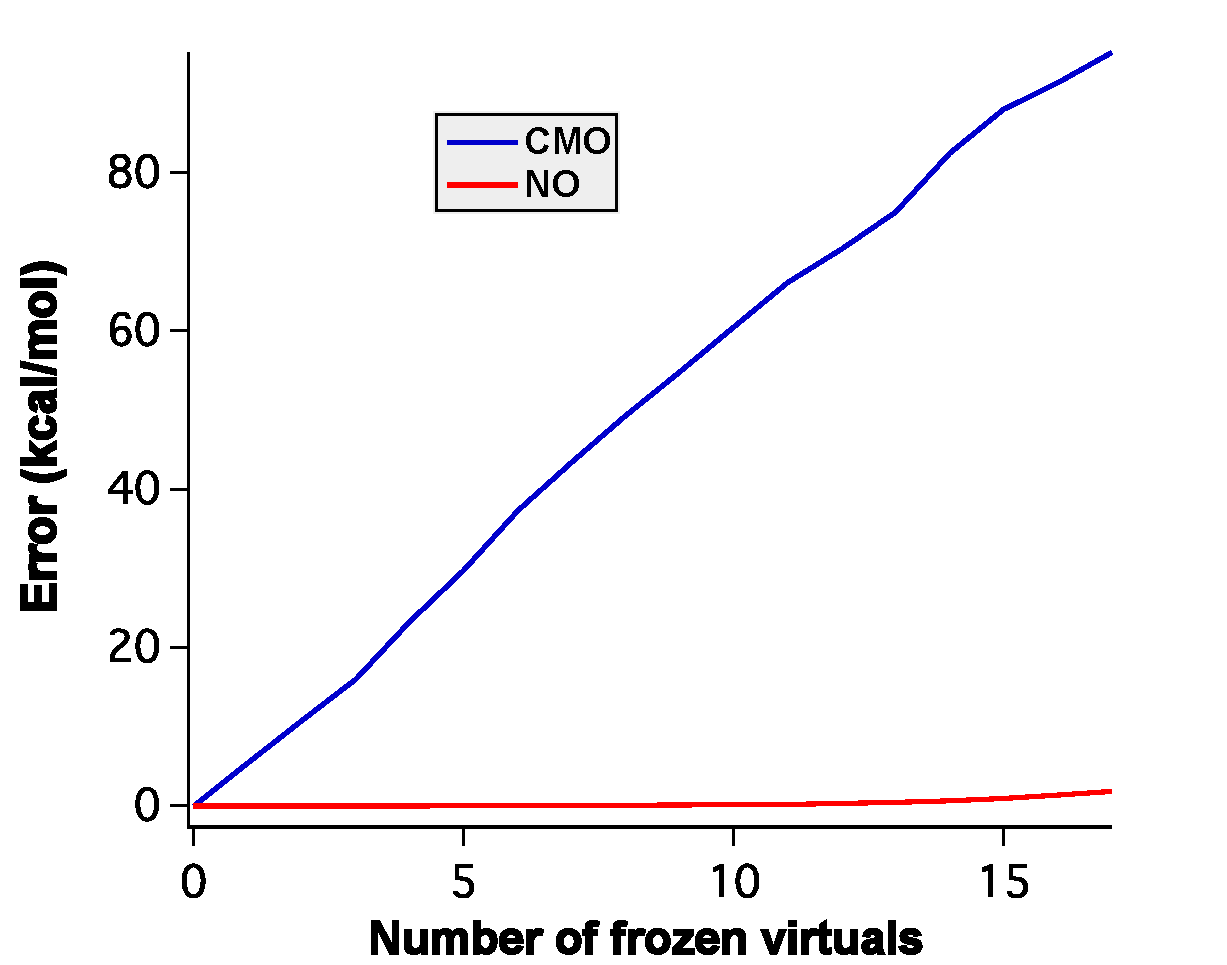
\includegraphics[width=0.7\linewidth]{figures/energy.pdf}
  \caption{Error in the CCSD energy of H$_2$O$_2$ in kcal/mol as a 
           function of the number of frozen virtual orbitals in both CMO and NO bases.} 
  \label{fig:energy}
\end{figure}
%%%%%%%%%%%%%%%%%%%%%%%%%%%%%%%%%%%%%%%%%%%%%%%%%%%%%%%%%%%%%%%
\begin{figure}
  \centering
  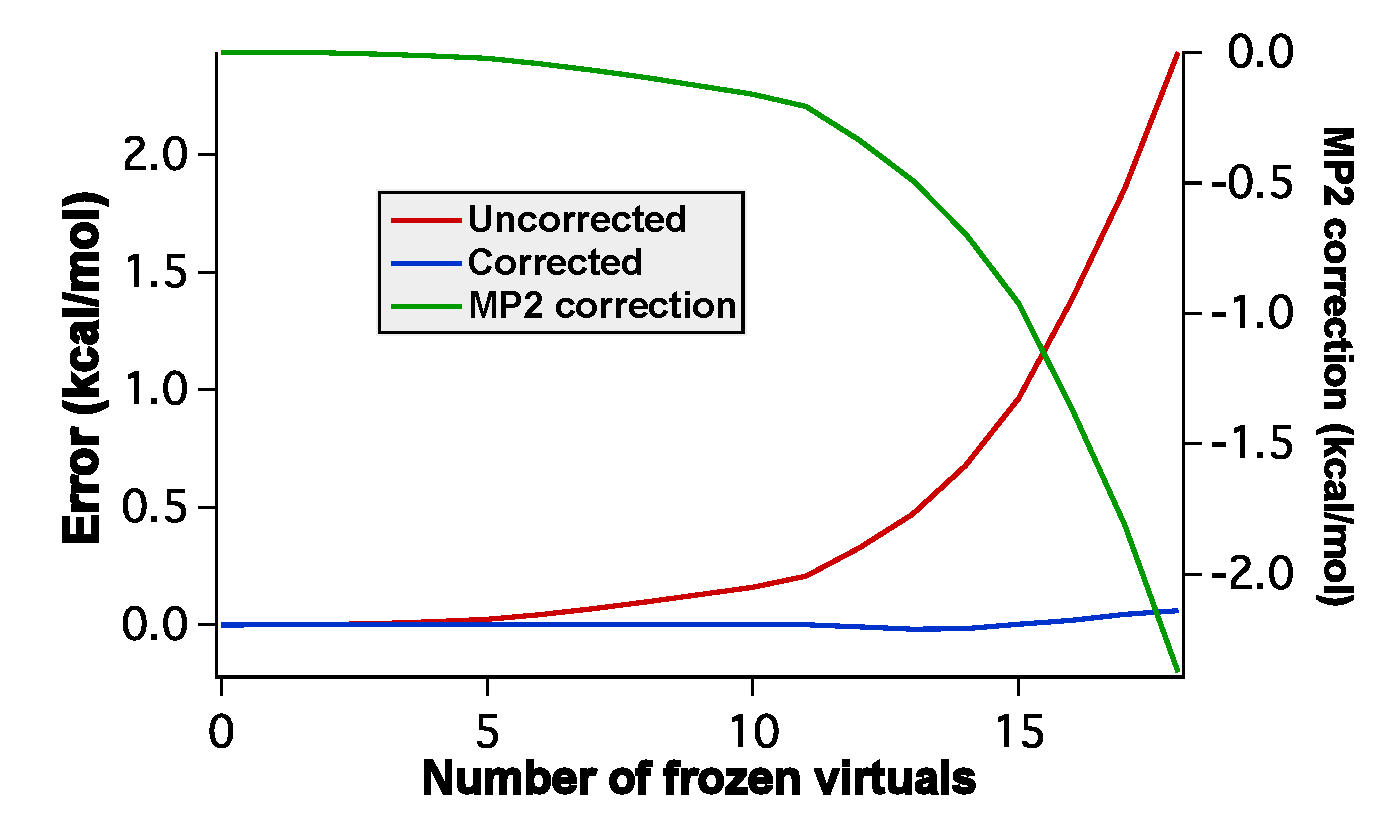
\includegraphics[width=0.7\linewidth]{figures/Mp2c.pdf}
  \caption{Error in CCSD energy of H$_2$O$_2$ in the NO bases, with and without MP2 corrections 
        and MP2 correction as a function of the number of frozen virtual orbitals.}
\label{fig:MP2_corr}
\end{figure}
%%%%%%%%%%%%%%%%%%%%%%%%%%%%%%%%%%%%%%%%%%%%%%%%%%%%%%%%%%%%%%%
\begin{figure}
  \centering
  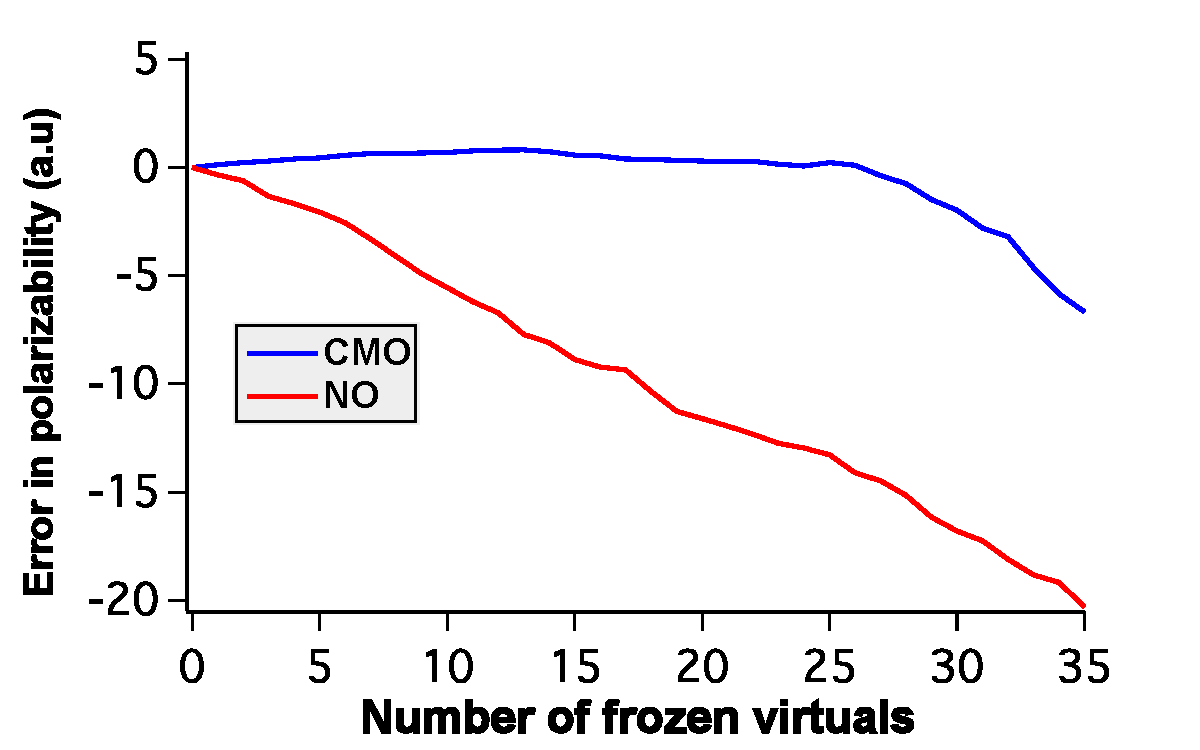
\includegraphics[width=0.6\linewidth]{figures/h2o2_polar.pdf}
  \caption{Errors in the CCSD/aDZ dynamic polarizability (589
nm) of H$_2$O$_2$ in 
       in both CMO and NO bases as a function of number of virtual orbitals removed.}
   \label{fig:polar_h2o2}
\end{figure}
%%%%%%%%%%%%%%%%%%%%%%%%%%%%%%%%%%%%%%%%%%%%%%%%%%%%%%%%%%%%%%%
\begin{figure}
  \centering
  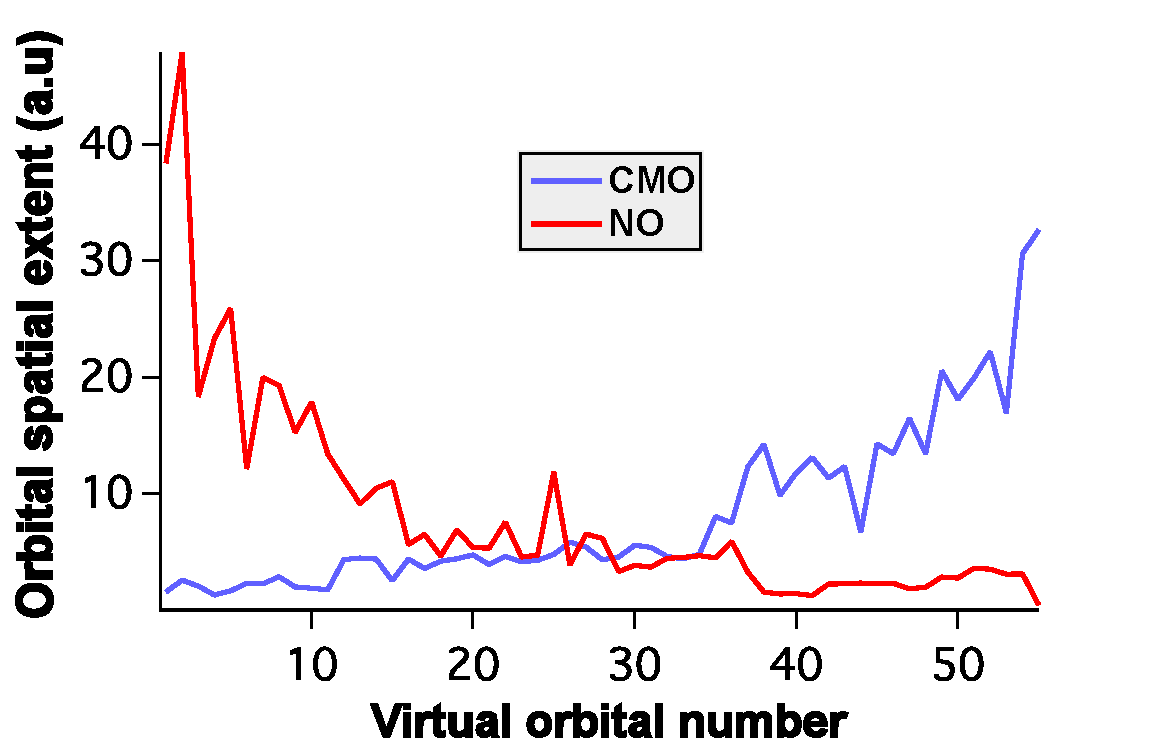
\includegraphics[width=0.6\linewidth]{figures/spatial.pdf}
  \caption{Spatial extent ($\langle r^2\rangle$) of virtual
orbitals of H$_2$O$_2$ in both CMO and NO bases.  Orbitals are ordered
left-to-right by
decreasing energy (CMOs) or increasing occupation number (NOs).}
   \label{fig:spatial}
\end{figure}

%%%%%%%%%%%%%%%%%%%%%%%%%%%%%%%%%%%%%%%%%%%%%%%%%%%%%%%%%%%%%%%
\begin{figure}
  \centering
  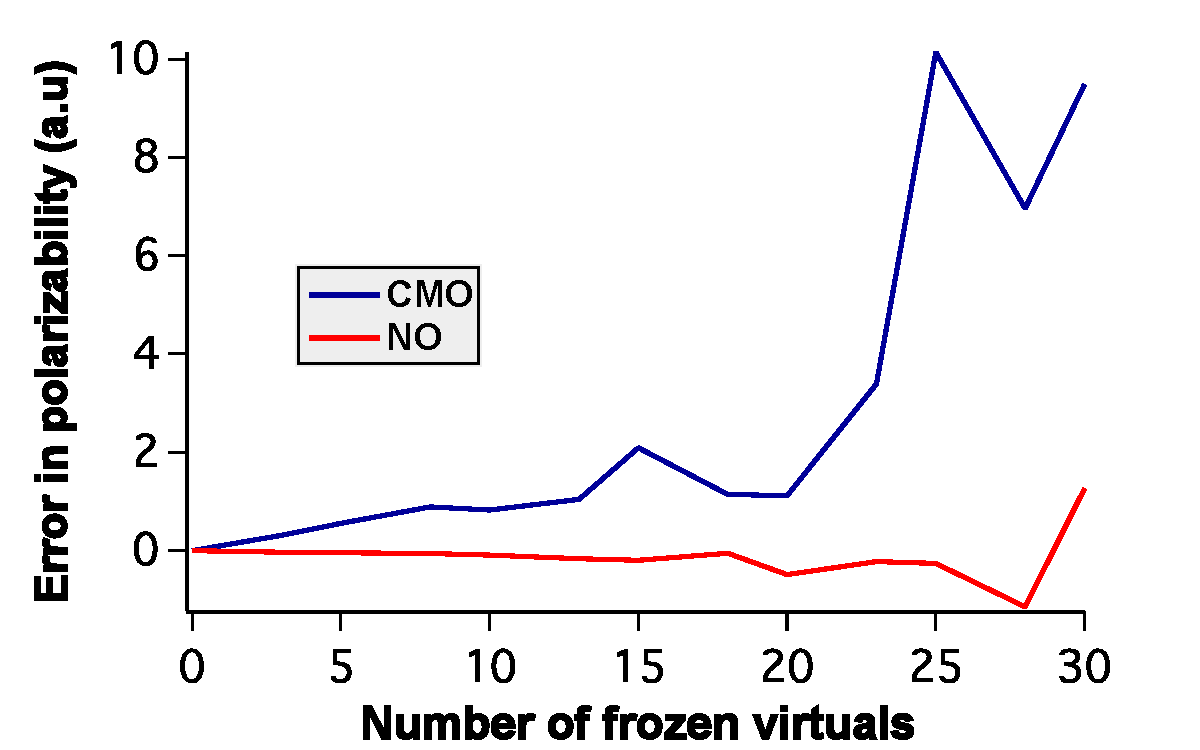
\includegraphics[width=0.6\linewidth]{figures/polar_static.pdf}
  \caption{Errors in the CCSD/aDZ static polarizability 
(including orbital relaxation effects) of H$_2$O$_2$ in
       in both CMO and NO bases as a function of number of virtual orbitals
removed.}
   \label{fig:static}
\end{figure}

%%%%%%%%%%%%%%%%%%%%%%%%%%%%%%%%%%%%%%%%%%%%%%%%%%%%%%%%%%%%%%%
\begin{figure}
  \centering
  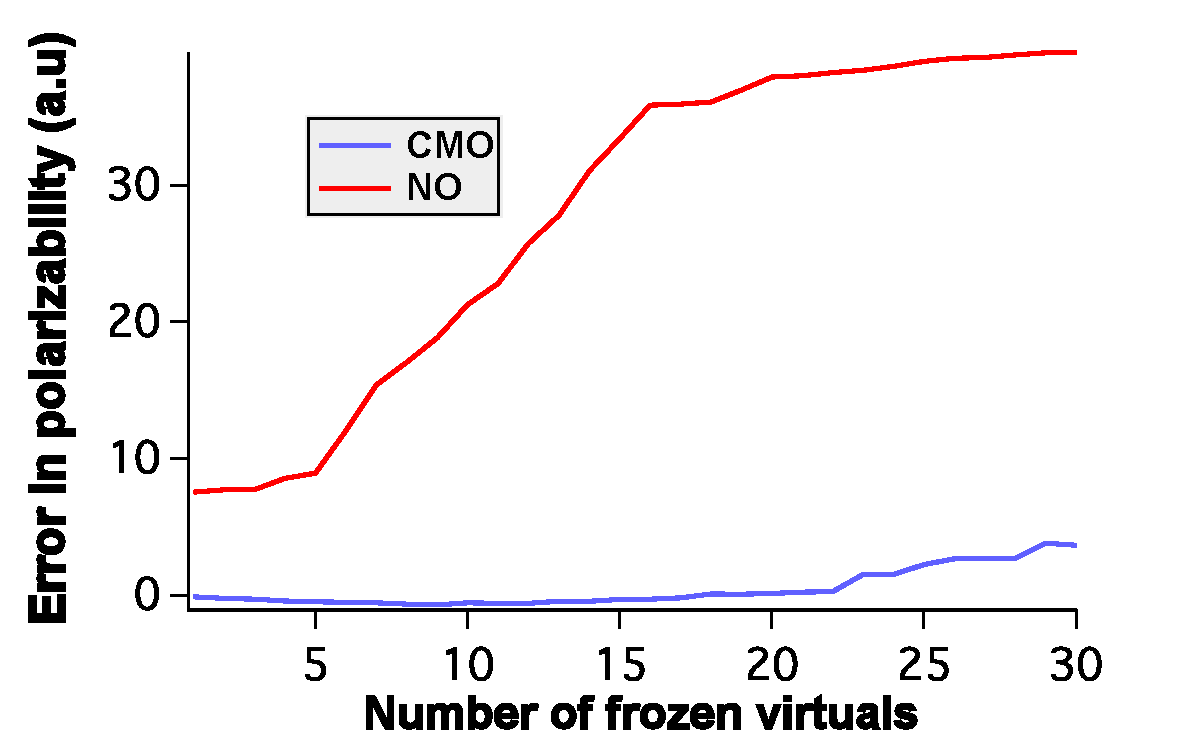
\includegraphics[width=0.6\linewidth]{figures/sort_spatial.pdf}
  \caption{Errors in the CCSD/aDZ dynamic polarizability (589
nm) of H$_2$O$_2$ as a function of the number of virtual CMOs or NOs deleted,
ordered by increasing spatial extent, $\langle r^2 \rangle$.}
   \label{fig:sort_spatial}
\end{figure}
%%%%%%%%%%%%%%%%%%%%%%%%%%%%%%%%%%%%%%%%%%%%%%%%%%%%%%%%%%%%%%%
\begin{figure}
  \centering
  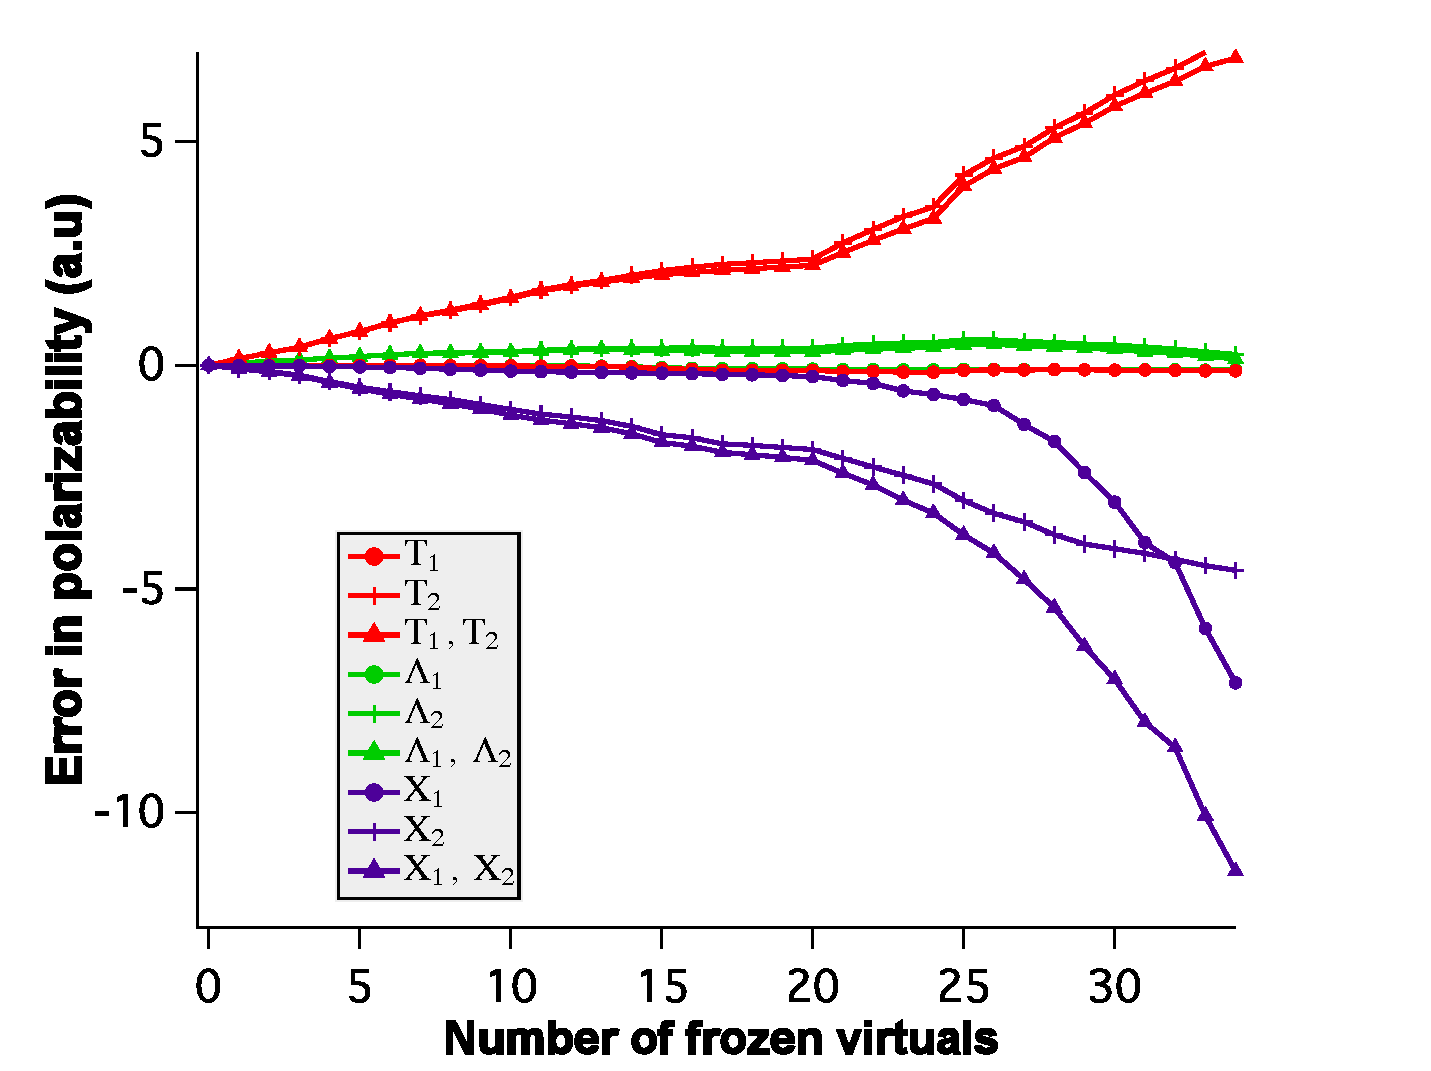
\includegraphics[width=0.6\linewidth]{figures/amp_trunc_cmo.pdf}
  \caption{Errors introduced in CCSD/aDZ polarizabilities of
H$_2$O$_2$ in the virtual CMO bases by the truncation of different classes of wave
function amplitudes.}
   \label{fig:amp_trunc_cmo}
\end{figure}
%%%%%%%%%%%%%%%%%%%%%%%%%%%%%%%%%%%%%%%%%%%%%%%%%%%%%%%%%%%%%%%
\begin{figure}
  \centering
  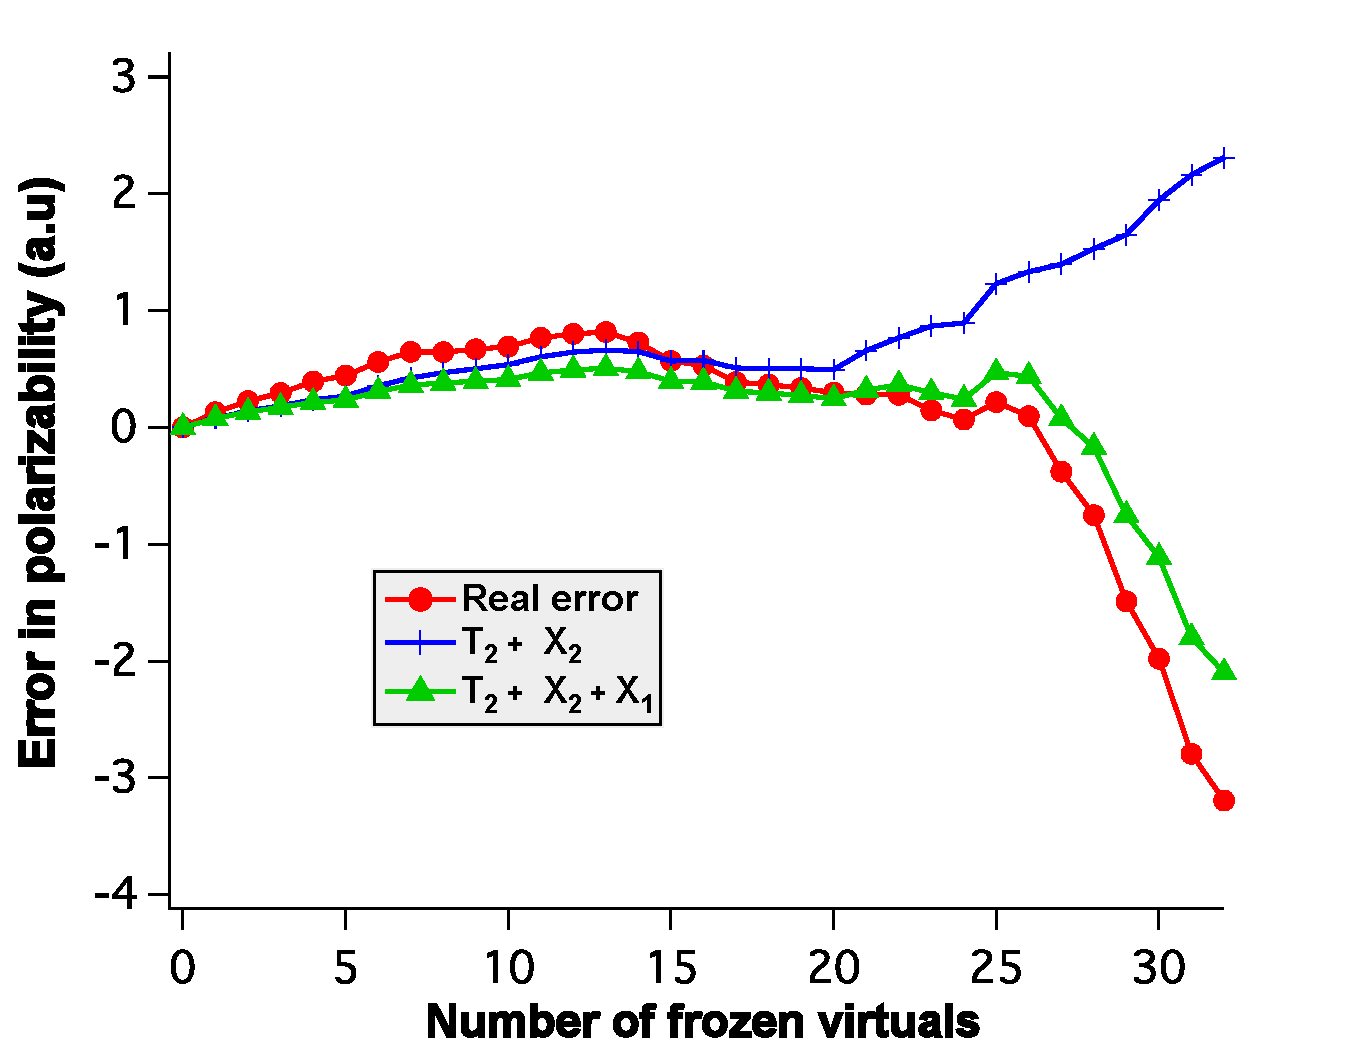
\includegraphics[width=0.6\linewidth]{figures/error_cmpare.pdf}
  \caption{Errors introduced in CCSD/aDZ polarizabilities of
H$_2$O$_2$ in the virtual CMO bases by the truncation of specific classes of wave
function amplitudes as compared to the total errors obtained by freezing of
virtual CMOs.}
   \label{fig:error_compare}
\end{figure}
%%%%%%%%%%%%%%%%%%%%%%%%%%%%%%%%%%%%%%%%%%%%%%%%%%%%%%%%%%%%%%%
\begin{figure}
  \centering
  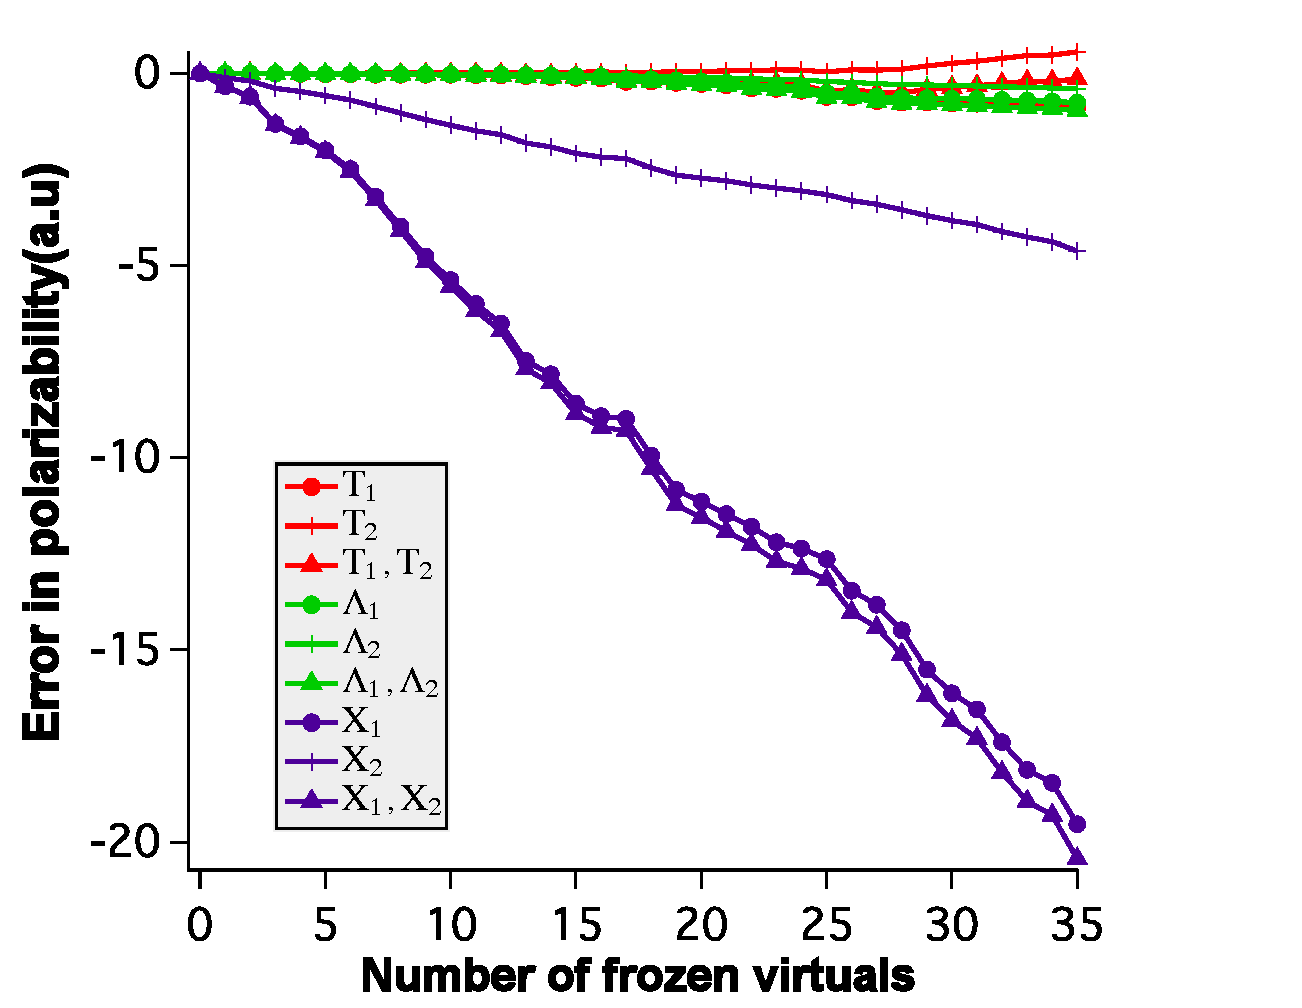
\includegraphics[width=0.6\linewidth]{figures/amp_trunc_no.pdf}
  \caption{Errors introduced in CCSD/aDZ polarizabilities of
H$_2$O$_2$ in the virtual NO bases by the truncation of different classes of wave
function amplitudes.}
   \label{fig:amp_trunc_no}
\end{figure}
%%%%%%%%%%%%%%%%%%%%%%%%%%%%%%%%%%%%%%%%%%%%%%%%%%%%%%%%%%%%%%%
\begin{figure}
  \centering
  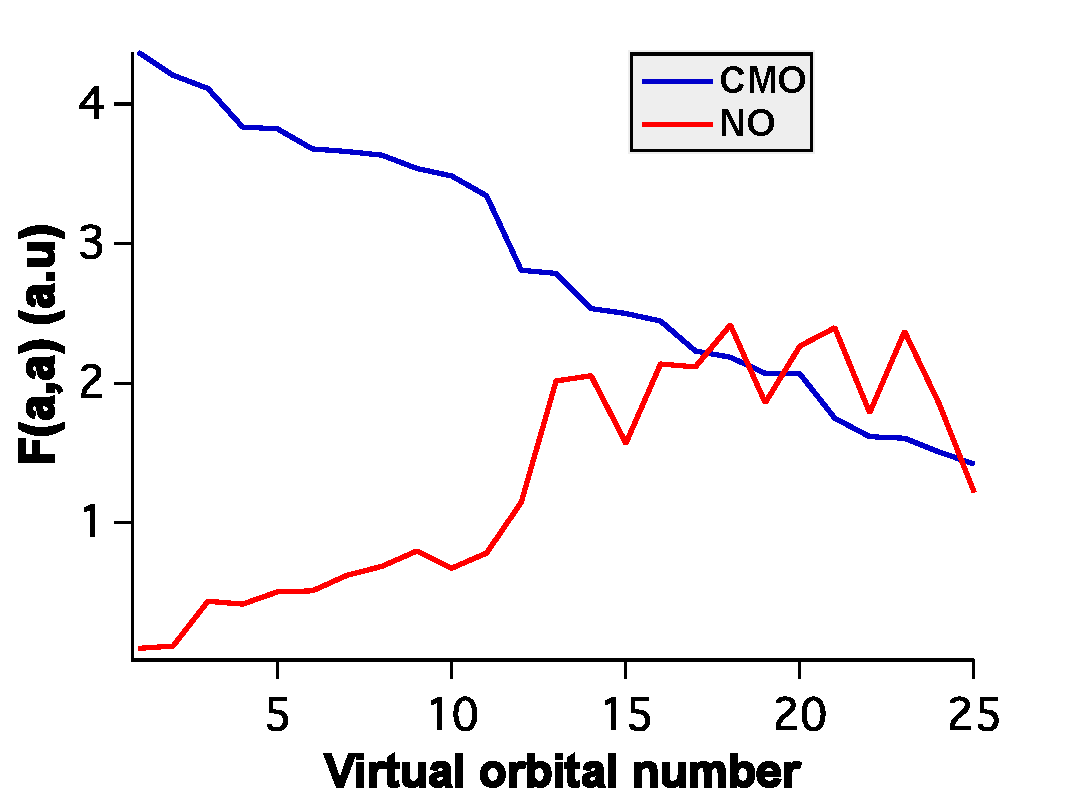
\includegraphics[width=0.6\linewidth]{figures/Faa.pdf}
  \caption{Virtual diagonal elements (a.u.) of the Fock matrix in
the CMO and NO bases.}
   \label{fig:Faa}
\end{figure}
%%%%%%%%%%%%%%%%%%%%%%%%%%%%%%%%%%%%%%%%%%%%%%%%%%%%%%%%%%%%%%%
\begin{figure}
  \centering
  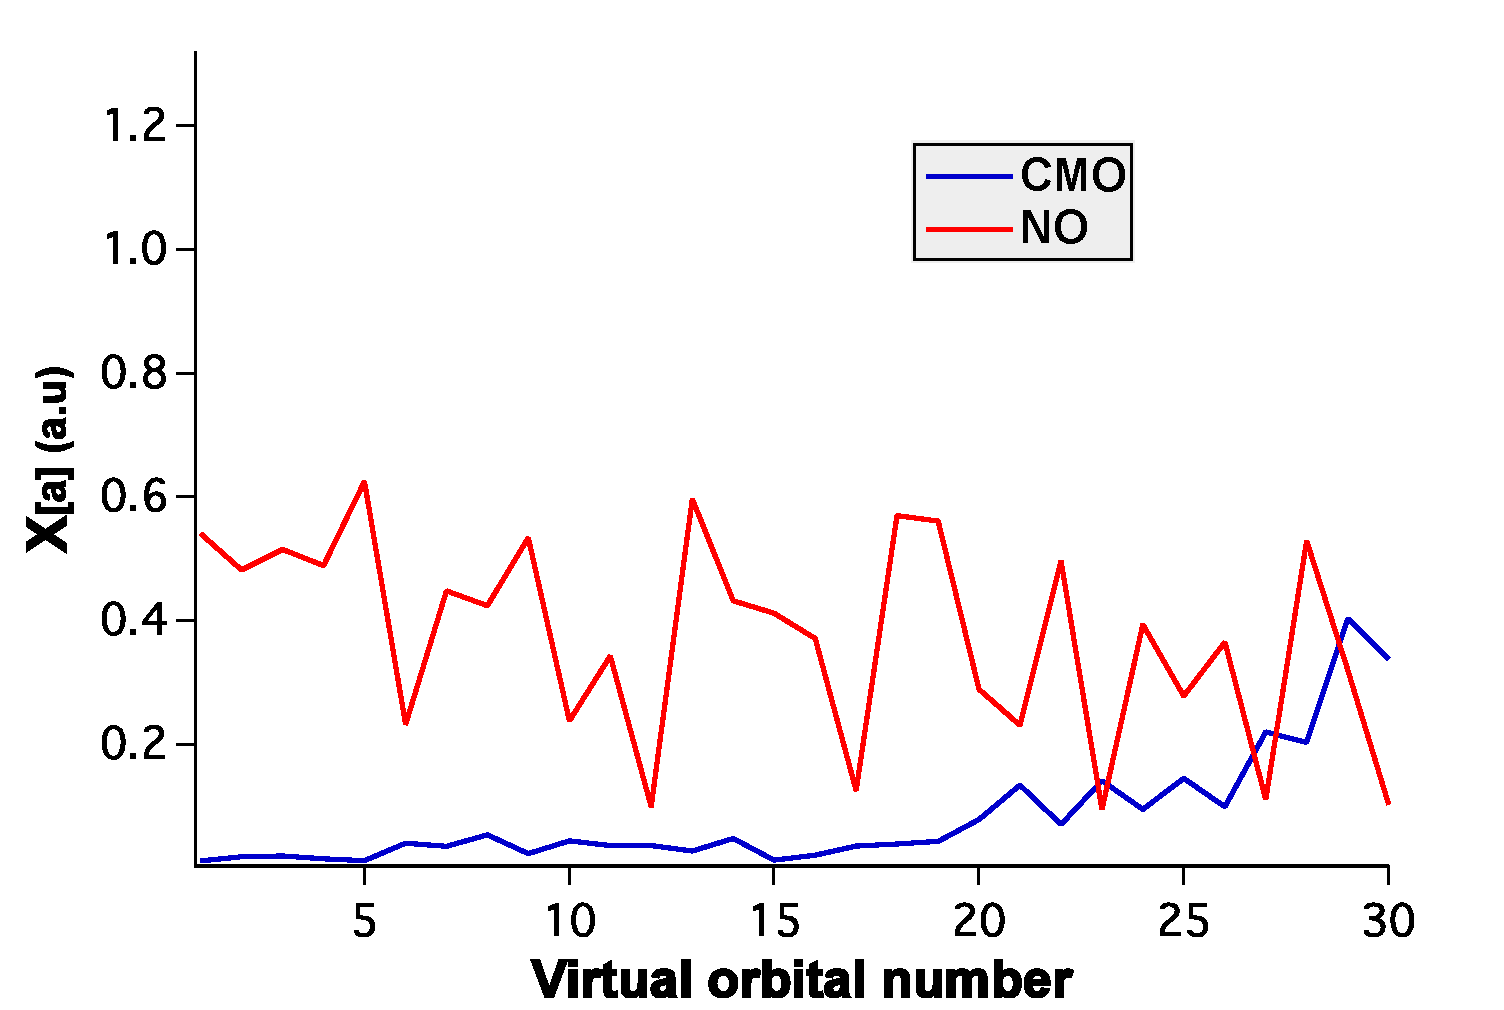
\includegraphics[width=0.6\linewidth]{figures/X1.pdf}
  \caption{Sum of the absolute values of $\hat{X}_1$
amplitudes for a given virtual, $\sum_i \left|X_i^a\right|$, for perturbation $\mu_x$
and frequency 589 nm, plotted for each virtual NO or CMO.}
   \label{fig:X1}
\end{figure}
%%%%%%%%%%%%%%%%%%%%%%%%%%%%%%%%%%%%%%%%%%%%%%%%%%%%%%%%%%%%%%%
\begin{figure}
  \centering
  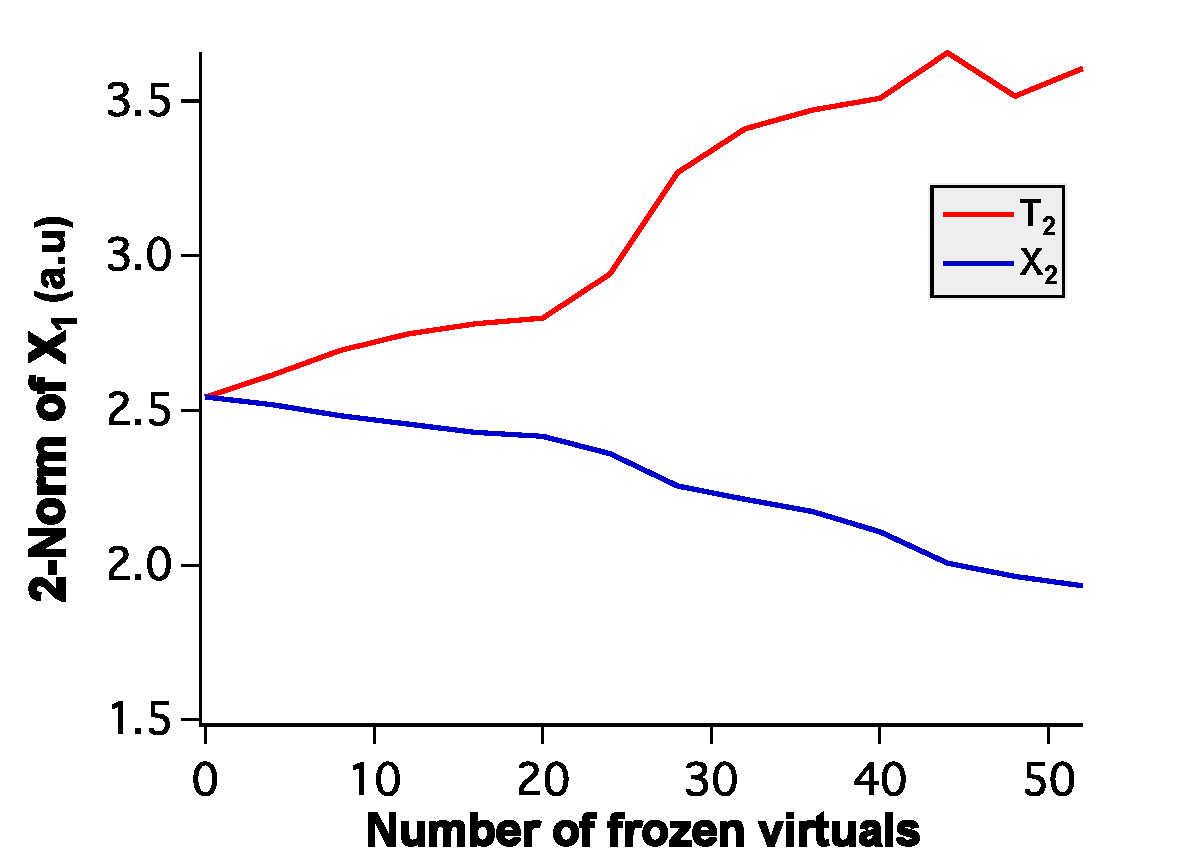
\includegraphics[width=0.6\linewidth]{figures/norm.pdf}
  \caption{The 2-norm of the $\hat{X}_1$ amplitude vector in
the CMO bases as a function of the truncation of classes of unperturbed 
$\hat{T}_2$ and perturbed $\hat{X}_2$ amplitudes.}
   \label{fig:norm}
\end{figure}
%%%%%%%%%%%%%%%%%%%%%%%%%%%%%%%%%%%%%%%%%%%%%%%%%%%%%%%%%%%%%%%
%\begin{figure}
%  \centering
%  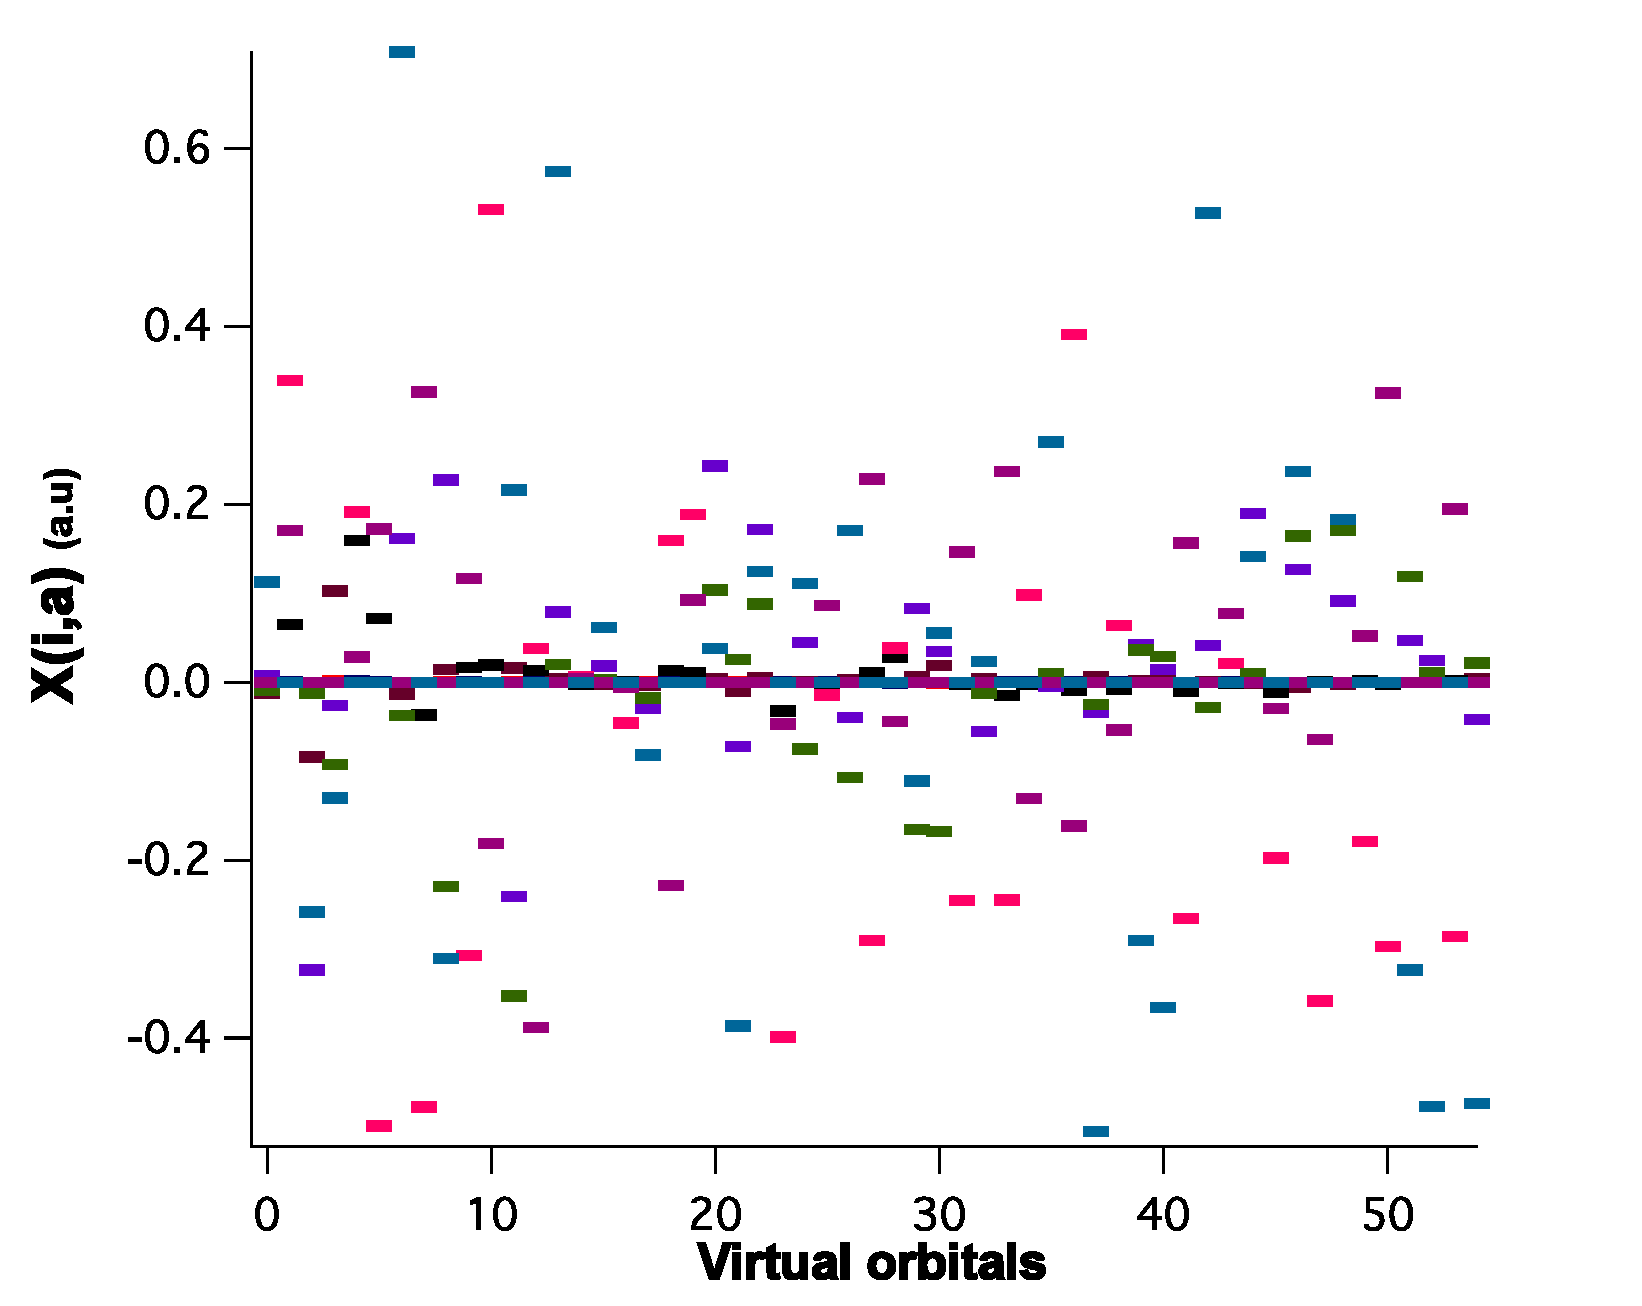
\includegraphics[width=0.6\linewidth]{figures/X1_no.pdf}
%  \caption{\footnotesize{$X_1$ amplitudes $X^{\mu_x}_{ia}$(589 nm) in the NO basis. For each virtual orbital there are nine virtual-occupied pairs.}}
%   \label{fig:X1_no}
%\end{figure}
%%%%%%%%%%%%%%%%%%%%%%%%%%%%%%%%%%%%%%%%%%%%%%%%%%%%%%%%%%%%%%%
\begin{figure}
  \centering
  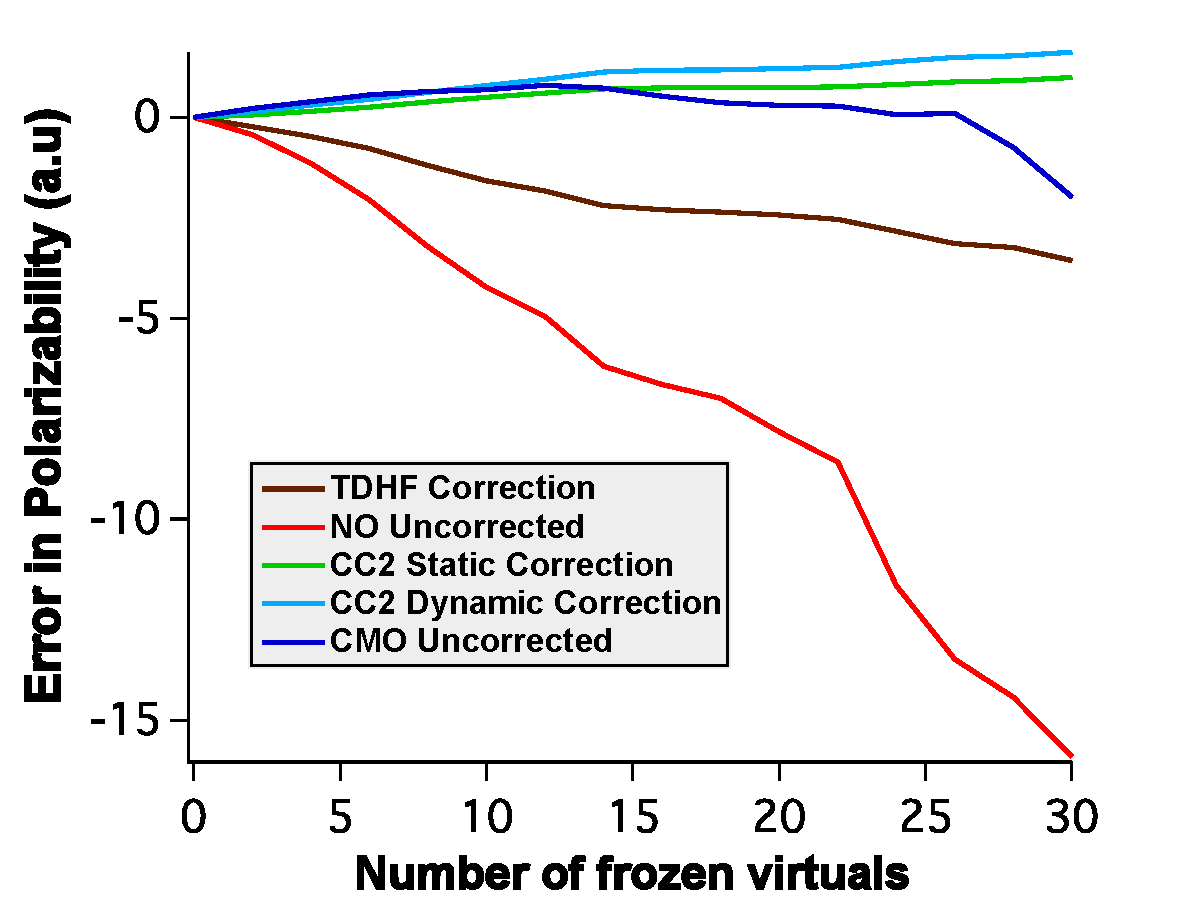
\includegraphics[width=0.6\linewidth]{figures/correctn.pdf}
  \caption{Correction schemes for the external truncated
NO space for the CCSD/aDZ polarizabilities of H$_2$O$_2$.}
   \label{fig:corrections}
\end{figure}
%%%%%%%%%%%%%%%%%%%%%%%%%%%%%%%%%%%%%%%%%%%%%%%%%%%%%%%%%%%%%%%

\begin{figure}
  \centering
  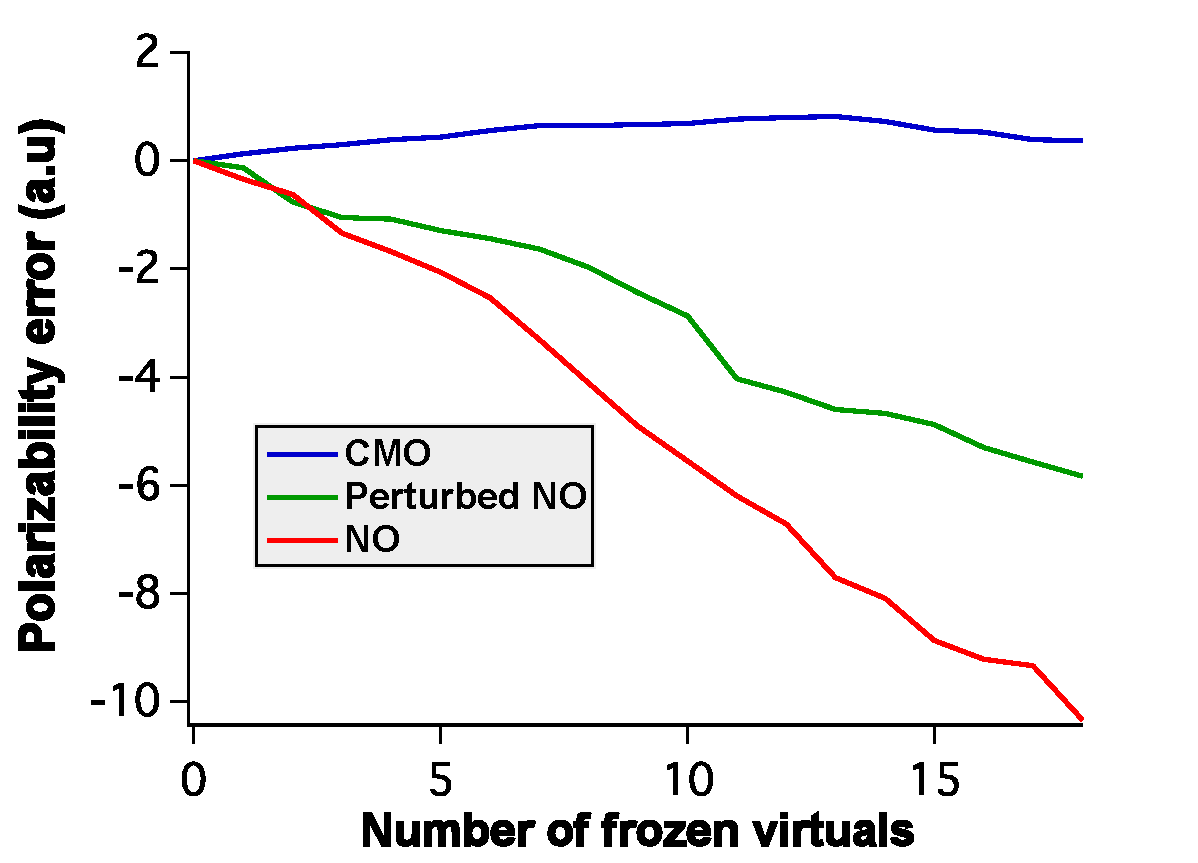
\includegraphics[width=0.6\linewidth]{figures/perturbed.pdf}
  \caption{Errors introduced in CCSD/aDZ polarizabilities of
H$_2$O$_2$ in the virtual CMO and NO bases, as well as the perturbed
virtual NO basis as a function of number of virtual orbitals removed.}
   \label{fig:perturb}
\end{figure}
%%%%%%%%%%%%%%%%%%%%%%%%%%%%%%%%%%%%%%%%%%%%%%%%%%%%%%%%%%%%%%%
\begin{figure}
  \centering
  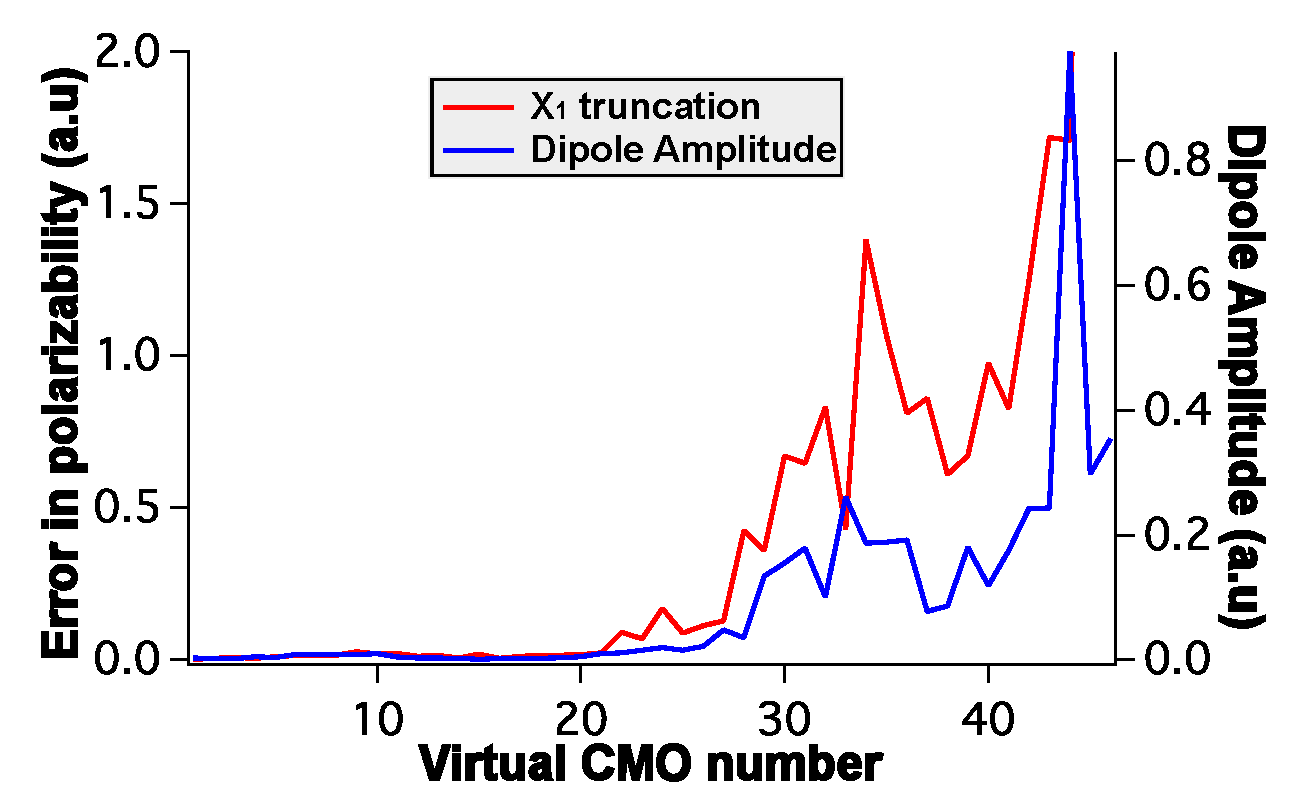
\includegraphics[width=0.6\linewidth]{figures/diplength.pdf}
  \caption{Absolute errors introduced in CCSD/aDZ
  polarizabilities of H$_2$O$_2$ due to truncation of $\hat{X}_1$ amplitudes and
  dipole amplitudes plotted as a function of different virtual CMOs.}
   \label{fig:dipole_length}
\end{figure}
%%%%%%%%%%%%%%%%%%%%%%%%%%%%%%%%%%%%%%%%%%%%%%%%%%%%%%%%%%%%%%%


\newpage
\begin{center}
{\bf TOC Graphic}
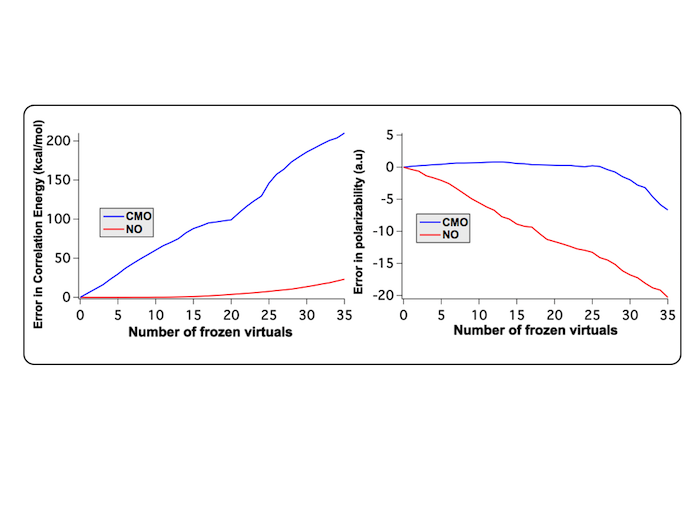
\includegraphics[width=1.0\linewidth]{figures/toc.png}
\end{center}


\end{document}

\chapter{Perturbed Natural Orbitals for Coupled-Cluster Linear-Response Theory}
\markright{Ashutosh Kumar \hfill Chapter 4. Perturbed Natural Orbitals  \hfill}
%\documentclass[journal=jpccck,manuscript=article]{achemso}
%\usepackage[numbers,super]{natbib}
%
%\usepackage{graphicx}
%\usepackage{xcolor}
%\usepackage{todonotes}
%
%\def\ket#1{| #1 \rangle}
%\def\bra#1{\langle #1 |}
%
%\usepackage[utf8]{inputenc} % set input encoding (not needed with XeLaTeX)
%\usepackage{verbatim}
%\usepackage{amsfonts}
%\usepackage{graphicx}
%\newcommand{\overbar}[1]{\mkern 2.2mu\overline{\mkern-2.2mu#1\mkern-2.2mu}\mkern 2.2mu}
%\usepackage{multirow}
%\usepackage{array}
%\usepackage{varwidth}
%\usepackage{bm}
%
%\title{Frozen Virtual Natural Orbitals ++ for Coupled Cluster Linear-Response Theory}
%\author{Ashutosh Kumar}
%\affiliation{Department of Chemistry, Virginia Tech, Blacksburg, Virginia 24061, U.S.A.}
%\author{T.\ Daniel Crawford}
%\email{crawdad@vt.edu}
%\affiliation{Department of Chemistry, Virginia Tech, Blacksburg, Virginia 24061, U.S.A.}
%
%\date{\today}
%
%\begin{document}
%
%\begin{abstract} We present here the the modified frozen-virtual natural-orbital (NO) 
%approach, which we call FVNO++ for a compact representation of the 
%response of the coupled cluster wavefunction to external electric
%and magnectic fields. In our earlier work,\cite{Kumar17}
%we showed that the regular FVNO method performs rather poorly for 
%%The frozen-virtual natural-orbital (NO) approach, whereby the
%%unoccupied-orbital space is constructed using a correlated density such as
%%that from many-body perturbation theory, has proven to yield compact wave
%%functions for determining ground-state correlation energies and associated
%%properties, with corresponding occupation numbers providing a guide to the
%%truncation of the virtual space.  In this work this approach is tested for the
%%first time for the calculation of higher-order response properties,
%%particularly frequency-dependent dipole polarizabilities using coupled-cluster
%%theory.  We find that such properties are much more sensitive to the
%%truncation of virtual space in the natural orbital (NO) basis than in the
%%original canonical molecular orbital (CMO) basis, with truncation errors
%%increasing linearly with respect to the number of frozen virtual NOs.  The
%%reasons behind this poor performance include the more diffuse nature of NOs
%%with low occupation numbers as well as the reduction in sparsity of the
%%perturbed singles amplitudes in the NO basis and the neglect of orbital
%%response.  We tested a number of approaches
%%to improve the performance of the NO space, including the use of a
%%field-perturbed density to define the virtual orbitals and various
%%external-space corrections.  The truncation of the CMO space, on the other
%%hand, yields errors in coupled-cluster dipole polarizabilities of less than
%%2\% even after removing as much as 50\% of the full virtual space. We find
%%that this positive performance of the CMO space results from a cancellation of
%%errors due to the truncation of the unperturbed and perturbed amplitudes, as
%%well as sparsity of the singles amplitudes.  We introduce a simple criterion
%%called a dipole amplitude to use as a threshold for truncating the CMO basis
%%for such property calculations.  \end{abstract}
%\end{abstract}
%\maketitle

\section{Introduction}

One of the central problems limiting the application of accurate {\em ab
initio} methods like coupled-cluster (CC) theory to large molecular systems is their high 
computational costs, i.e., their computing and storage requirements 
exhibit polynomial scaling with the size of the system or equivalently
with the number of one electron basis functions used in these calculations.
Specifically, the size of the virtual space is of greater concern since  
they usually far outnumber the occupied orbitals. Furthermore, the canonical virtual orbitals
obtained from the Hartree-Fock (HF) procedure are non-local in nature and hence 
the convergence of a determinantal expansion involving these orbitals
is quite slow. However, L{\"o}wdin \cite{}showed that using 
``natural orbitals'' (NOs) instead of canonical HF orbitals can significantly 
accelerate the convergence of the configuration interaction (CI)
wavefunction expansion. The NOs are the eigenvectors of the 
1 electron reduced density matrix (1-RDM) associated with a wavefunction. 
The corresponding eigenvalues are commonly referred to 
as ``occupation numbers''. Since L{\"o}wdin's pioneering 
work, NOs have found a lot of applications especially in techniques 
aimed at obtaining a compact representation of the virtual space for 
correlated calculations.\cite{} Please refer to ref. \cite{Landau10}
for an excellent overview on this subject. Within the context of the CC theory, 
the frozen virtual NO (FVNO) scheme where the NOs are usually obtained from 
the 1-RDM of a less expensive correlated method such as second-order 
M{\"o}ller-Plesset (MP2) theory and the virtual space for subsequent 
CC calculations is truncated based on the orbitals' occupation 
numbers has been used quite successfully to calculate correlation energies, 
ionization enthalpies etc\cite{}. For example, Landau et al.\cite{} demonstrated 
that even after the removal of 70\% of the virtual space, the errors in
the ionization energies of organic compounds were less than 1 kcal/mol.
However, it has been well established from previous studies that response 
properties are usually much more sensitive to the truncation of the wavefunction 
than simple energetics\cite{}. So we investigated the applicability of such 
approaches for properties like dynamic polarizabilities using CC linear reponse theory
\cite{}. In contrast to the earlier studies, we got huge errors in polarizabilities 
which increased almost linearly with the number of truncated virtual orbitals. 
It was found that the ground-state MP2 density used to generate the NOs was 
unable to capture the response of the wavefunction to the external field. 
For example, the FVNO procedure threw out first, the diffuse virtual 
orbitals which are very important to describe the low lying Rydberg type 
excited states (a common feature in majority of chiral compounds) 
resulting in large errors. This was not unsurprising since these diffuse 
orbitals have very low contributions to the correlation energy and hence 
possess very low occupation numbers. Consistent with the findings of Sundholm 
and co-workers\cite{Sundholm13}, dropping high energy canonical HF 
virtual orbitals led to very small errors in polarizabilities. 
We also constructed a first-order perturbed MP2 density hoping that 
the ONs obtained from this density would be a better metric for 
estimating the importance of a virtual orbital 
for response properties but this approach only offered
minor improvements over the regular FVNO method. However, 
a suite of methods, conceptually not very different from our 
perturbed density approach have been proposed recently 
to calculate CC excitation energies. Baudin and co-workers 
used natural transition orbitals (NTOs) obtained from approximate 
CIS(D) transition densities, a scheme which they call CorNFLEx for 
calculating CC2 excitation energies of large solvated formamide 
clusters\cite{}. In similar works, H{\"o}fener and Klopper 
obtained effective virtual spaces by combining MP2 
ground state density with excited state densities constructed from CIS 
excitation vectors\cite{} while Mester et al. used MP2 and CIS(D) amplitudes 
to define their optimal virtual and occupied spaces\cite{Mester17,Mester18}.
These successful works prompted us to take back a closer look at the 
reasons behind the failure of our perturbed density approach. 
Finally, we have developed a new method which we call FVNO++ 
where we construct a second-order perturbed density to 
capture the response of the wavefunction to the external electric 
and magnetic fields. In this paper, we look at some of the basis aspects of 
this method and report its performance in calculating CC dynamic 
polarizabilities and specific rotations of a number of chiral molecules .
\section{Theoretical Background}
%\subsection{Frozen Virtual Natural Orbitals}
%The MP2 unrelaxed one-electron density matrix can be written in terms of
%spin orbitals as: 
%\begin{equation}
%\gamma_{pq} = \langle \Psi^{(1)}|\{ a^{\dagger}_{p}a_q\}|\Psi^{(1)}\rangle,
%\label{Eq:density}
%\end{equation}
%where $|\Psi^{(1)}\rangle$ is the first order correction to the Hartree-Fock
%wave function,
%\begin{equation}
%|\Psi^{(1)}\rangle = \frac{1}{4}\sum_{ijab} t^{ab}_{ij}|\Phi^{ab}_{ij}\rangle
%\end{equation}
%and
%\begin{equation}
%t^{ab}_{ij} = \frac{\langle ij||ab\rangle}{\epsilon_i + \epsilon_j -
%\epsilon_a - \epsilon_b}.
%\end{equation}
%Here, $\langle ij||ab\rangle$ is an antisymmetrized two-electron integral in
%Dirac's notation and $\epsilon_i,\epsilon_a...$ refer to the Hartree-Fock
%molecular orbital energies. We use the indices $i,j,k,...$ to indicate occupied
%orbitals while $a,b,c,...$ denote virtual orbitals. $|\Phi^{ab}_{ij}\rangle$
%refers to a doubly-excited determinant where occupied orbitals $i$ and $j$ are
%replaced by virtuals $a$ and $b$ respectively.  The brackets around the
%second-quantized operators in Eq.~(\ref{Eq:density}) indicate normal ordering
%with respect to the reference wave function.
%
%In the MP2 based NO method, the virtual-virtual block of $\gamma_{pq}$
%is constructed,
%\begin{equation}
%\gamma_{ab} = \frac{1}{2}\sum_{ijc} t^{ac}_{ij}t^{bc}_{ij},
%\label{Eq:dens}
%\end{equation}
%and then diagonalized,
%\begin{equation}
%\bm{\gamma} \bm{V} = \bm{n} \bm{V}.
%\end{equation}
%The eigenvectors, $\bm{V}$, are the virtual natural orbitals (NOs), and the
%eigenvalues, $\bm{n}$, are the associated occupation numbers.  As noted
%earlier, the wave function amplitudes contain significantly greater sparsity
%when represented in the NO basis than the original canonical MO basis;
%orbitals with lower occupation numbers yield $\hat{T}_2$ amplitudes with
%smaller magnitudes and concomitantly smaller contributions to the correlation
%energy.  Thus, orbitals with occupation numbers below a selected threshold can
%be removed without introduction of significant errors, leading to reduced
%computational cost.  The Hartree-Fock virtual molecular orbitals and
%associated integrals are then transformed to this truncated NO basis, followed
%by semicanonicalization of the virtual-virtual block of the Fock matrix, for
%subsequent computations using higher-order correlation methods such as CC
%theory.  In most cases, the final correlation energy in the truncated virtual
%space is corrected using the MP2 energy in the external (non-truncated) NO
%space to minimize the resulting errors, as described belowa

\subsection{Coupled Cluster Response Theory}
The response functions for calculating dynamic higher-order properties 
are defined by the frequency dependent coefficients 
appearing in the expansion of the expectation value of an appropriate 
time-independent operator in orders of the perturbation.
\begin{equation}
A(t) = \langle \Psi^{(0)} | \hat{A} | \Psi^{(0)} \rangle \
+ \langle \Psi^{(1)}(t) | \hat{A} | \Psi^{(0)} \rangle\
+ \langle \Psi^{(0)} | \hat{A} | \Psi^{(1)}(t) \rangle\ 
+ \langle \Psi^{(1)}(t) | \hat{A} | \Psi^{(1)}(t) \rangle + ... \\
\end{equation}
For example, the linear reponse function ${\langle\langle A;B\rangle\rangle}_{\omega_1} $ 
can be seen as the first order change in the expectation value of $\hat{A}$ in 
the time-dependent field parametrized by the operator $B$,
\begin{equation}
\int_{-\infty}^{\infty}d\omega_1{\langle\langle A;\
B\rangle\rangle}_{\omega_1 + i\alpha}e^{(-i\omega_1 + \alpha)t} \
= \langle \Psi^{(1)}(t) | \hat{A} | \Psi^{(0)} \rangle\
+ \langle \Psi^{(0)} | \hat{A} | \Psi^{(1)}(t) \rangle\
\end{equation}
One can obtain electric-electric ($\alpha$) and electric-magnetic ($\beta$)
dipole polarizability tensors from the linear response function with appropriate
operators,
\begin{equation}
\alpha_{xy}(\omega) = {\langle\langle \mu_x;\mu_y\rangle\rangle}_{\omega_1}
\end{equation}
\begin{equation}
\beta_{xy}(\omega) = {-\text{Im} \langle\langle \mu_x;m_y\rangle\rangle}_{\omega_1}
\end{equation}
where $\mu = \sum_i q_i r_i $ and $m = \sum_i \frac{q_i}{2m_i} r_i \times p_i$. 
One-third of the trace of the $\alpha$ tensor is the isotropic 
electric dipole polarizability. Specific rotation on the other hand 
is related to the one-third of the trace of the $\beta$ tensor (au) 
also known as the Rosenfeld tensor by the following expression\cite{},
\begin{equation}
{\lbrack\alpha\rbrack}_{\omega} = \frac{(72.0 \times 10^6){\hbar}^2 N_A\omega}{c^2{m_e}^2 M}
\ \times \left[ \frac{1}{3}Tr(\beta)\right]
\end{equation}
where M is the mass of the molecule (amu), $m_e$ is the rest mass of an electron
(kg), c is the speed if light in vacuum (m/s), $N_A$ is Avogadro's number and $\omega$
is the frequency of the electromagnetic field (au). \\
The coupled cluster linear response function can be written as\cite{}: 
\begin{equation}
{\langle\langle A;B\rangle\rangle}_{\omega_1} =  \langle \Psi_0 | \
[\hat{Y}^{B}_{\omega_1}, \bar{A}]|\Psi_0\rangle + \langle \Psi_0 | \
(1 + \hat{\Lambda})|[\bar{A},\hat{X}^{B}_{\omega_1}]|\Psi_0\rangle 
\end{equation}
where $A$ and $B$ are the one electron property operators,
$\omega_1$ is the frequency of the external field, 
$\Psi_0$ is the reference wavefunction, $\hat{\Lambda}$ is 
a linear de-excitation operator that parametrizes the CC left hand 
wavefunction to make sure that the CC gradients satisfy the 
generalized Hellman-Feynman theorem\cite{}, $\bar{A}$ is the 
similarity transformed $\hat{A}$ operator $\hat{A}$, $\bar{A} = e^{-\hat{T}}\hat{A}e^{\hat{T}}$,
$\hat{X}^{B}_{\omega_1}$ and $\hat{Y}^{B}_{\omega_1}$ are the first-order 
perturbed right and left hand amplitudes corresponding to perturbation operator 
$B$ respectively. 
\subsection{Perturbed Natural Orbitals}
The CC linear response function (eq. ) can also be formulated in terms of densities,
\begin{equation}
{\langle\langle A;B\rangle\rangle}_{\omega_1} =  \sum_{pq} A_{pq}D^{B}_{pq}(\omega_1)
\end{equation}
where $D^{B}(\omega_1)$ is the frequency dependent first-order
perturbed one-electron density related to operator B. The structures  
of the virtual-virtual block of the perturbed densities for a given
perturbation operator can be easily identified in spin orbitals as,
\begin{equation}
\begin{split}
%\begin{multline}
& D^{(0)}_{ab} = \frac{1}{2}(\lambda^{ij}_{ac})^{(0)}(t^{bc}_{ij})^{(0)} + (\lambda^{i}_{a})^{(0)}(t^{b}_{i})^{(0)} \\
&D^{(1)}_{ab} = \frac{1}{2}[(\lambda^{ij}_{ac})^{(0)}(t^{bc}_{ij})^{(1)} + (\lambda^{ij}_{ac})^{(1)}(t^{bc}_{ij})^{(0)}] + [(\lambda^{i}_{a})^{(0)}(t^{b}_{i})^{(1)} + (\lambda^{i}_{a})^{(1)}(t^{b}_{i})^{(0)}] \\
&D^{(2)}_{ab} = \frac{1}{2}[{(\lambda^{ij}_{ac}})^{(1)}(t^{bc}_{ij})^{(1)} + (\lambda^{ij}_{ac})^{(0)}(t^{bc}_{ij})^{(2)}]
\ + [(\lambda^{i}_{a})^{(1)} (t^{b}_{i})^{(1)} + (\lambda^{i}_{a})^{(0)}(t^{b}_{i})^{(2)}]\\
%\end{multline}
\end{split}
\end{equation}
In the above equation, the indices $i,j$ and $a,b,c$ refer to occupied and virtual orbitals respectively
and Einstein summation notation is used. The first order perturbed amplitudes $(\lambda^{ij}_{ac})^{(1)}$ 
and $(t^{bc}_{ij})^{(1)}$ are nothing but the $\hat{X}^{B}_{\omega_1}$ and $\hat{Y}^{B}_{\omega_1}$ 
amplitudes that we saw earlier.\\ Just as the ground state MP2 density can transfer its knowledge of 
electron correlation effects to the one electron basis (virtual NOs) through diagonalization, 
the perturbed densities can be used in a similar way to construct a compact ``perturbation aware''
basis. In our earlier work, we used a guess first-order perturbed density constructed from MP2 amplitudes
to obtain our virtual space but this approach offered only a minor improvement\cite{}.
To investigate the reason behind the failure of this model, we constructed the virtual-virtual
block of the full CCSD first-order perturbed density. All the diagonal elements of this density 
matrix were found to be zeros irrespective of the perturbation operator. The exact reason for this
is not yet understood but clearly, the NOs obtained from this (or guess) density doesn't carry any useful
information. However, since the polarizabilities are second-order in perturbation, second-order perturbed densities 
should in principle be a better metric for estimating the importance of a virtual NO for these properties.
In this paper, we use second-order guess densities to define our virtual space for correlated response calculations.
For a perurbation operator A,
\begin{equation}
{D^{'}(A)}^{(2)}_{ab} = \frac{1}{2}(t^{ac}_{ij}(A))^{(1)}(t^{bc}_{ij}(A))^{(1)} + (t^{a}_{i}(A))^{(1)} (t^{b}_{i}(A))^{(1)}, 
\end{equation}
where,
\begin{equation}
\begin{split}
& t^{ac}_{ij}(A)^{(1)} = \frac{-\bar{A}^{ac}_{ij}}{\epsilon_i + \epsilon_j - \epsilon_a - \epsilon_c},\\
& t^{a}_{i}(A)^{(1)} = \frac{-\bar{A}^{a}_{i}}{\epsilon_i - \epsilon_a}\\
\end{split}
\end{equation}
Here, we have used MP2 amplitudes for the similarity transformation, i.e. 
\begin{equation}
\bar{A}^{ac}_{ij} = P_{ij}^{ac}(t^{ec}_{ij}A^a_e - t^{ac}_{mj}A^m_i) ,
\end{equation}
ignored the terms involving second-order perturbed amplitudes and 
approximated the first-order perturbed $\lambda$ amplitudes by the 
corresponding $t$ amplitudes. The first-order right-hand perturbed
amplitudes in CC linear response theory can be expressed as, 
\begin{equation}
\begin{split}
& t^{ac}_{ij}(A)^{(1)}(\omega_1) = - \langle\Phi_{ij}^{ac}| {(\bar{H} -\omega_1 I)}^{-1} |
\Phi_{k\ldots}^{d\ldots}\rangle \langle \Phi_{k\ldots}^{d\ldots}| \bar{A} | \Phi_0\rangle, \\
& t^{a}_{i}(A)^{(1)}(\omega_1) = - \langle\Phi_{i}^{a}| {(\bar{H} -\omega_1 I)}^{-1} |
\Phi_{k\ldots}^{d\ldots}\rangle \langle \Phi_{k\ldots}^{d\ldots}| \bar{A} | \Phi_0\rangle \\
\end{split}
\end{equation}
It can be clearly seen that the guesses for $t^{ac}_{ij}(A)^{(1)}$ and 
$t^{a}_{i}(A)^{(1)}$ amplitudes in this work have been chosen by 
only considering the diagonal elements of $(\bar{H} -\omega_1 I)^{-1}$
which can be justified due to the diagonally dominant nature of the
$\bar{H}$ matrix. Furthermore, we keep $\omega_1$ as zero as we 
want to use the same density matrix for a given property calculation at different
frequencies. We also assume that removing $\omega_1$ should not significantly change the 
sparsity pattern of the perturbed amplitudes. 
\section{Computational Details}
1. primary application : optical rotation of solvated molecular clusters. But for pilot studies,
   (for the right behavior or tend)
   we chose chiral test cases - $h_2o_2$, linear (H2)n helices, phenylethanol, betapinene
   norbornenone 
2. properties - dynamic polarizabilities 
   and specific rotation. Polarizabilities mostly as a diagnostic tool
   because even though its linear response function is quite similar in structure
   to optical rotation, it is less sensitive to the truncation of the wavefunction.
  for polarizabilities - second-order guess densities based on a) elctric dipole,
  for specific rotation - b) magnetic dipole and c) both electric and magnetic dipoles
3. CC2 and CCSD method  - length and MVG - aug-cc-pvdz basis
4. sparsity plots of large solvated clusters (since we can't do full calculations 
	right now!) using densities constructed using density-fitting.
5. Psi4 and Psi4Numpy software used!
6. We have used the same virtual space for calculating both unperturbed and 
perturbed amplitudes as this ensures a match with results obtained 
from finite-field procedures.

%The r test cases of this work is hydrogen peroxide,
%H$_2$O$_2$, though additional tests are reported for related species such as
%(\textit{P})-dimethylallene and (\textit{S})-methyloxirane, as well as those
%same molecules interacting with one or more water molecules.  All molecular
%structures were optimized using the B3LYP
%functional\cite{Becke93,Stephens94:B3LYP,Lee88:LYP} in the aug-cc-pVDZ (aDZ)
%basis.\cite{Dunning89,Kendall92,Woon94} (Coordinates of all structures are
%provided in Tables S1-S5 of the Supporting Information.) Frequency-dependent
%polarizabilities were computed at the coupled cluster singles and doubles
%(CCSD) level of theory\cite{Purvis82} using a linear-response
%formulation.\cite{Christiansen98} While the aDZ basis set was used for most
%test calculations, the larger aug-cc-pVTZ (aTZ) and aug-cc-pVQZ (aQZ) basis
%sets were also employed for selected analyses.\cite{Kendall92} All orbitals
%were active in the correlated models utilized here, and all coupled-cluster
%calculations were carried out using the PSI4 open-source quantum chemistry
%package.\cite{psi4}  In all calculations in which virtual orbitals are
%truncated, the same orbital space is used in the solution of the unperturbed
%and perturbed amplitudes equations, just as is required for locally correlated
%property calculations.\cite{Crawford10}  We note that the size-extensivity of
%the polarizability is unaffected by the truncation of
%the virtual space.
%
\section{Results and Discussion}
Retention of diffuse space: Sort all the canonical MOs by their spatial
extents <i|r*r|i>, choose a cutoff, retain all the orbitals above that cutoff
and apply the regular FVNO in the remaining virtual space. As an example
for h2o2 in aug-cc-pvdz basis., we retained 26 out of 55 most diffuse virtual 
CMOs, constructed MP2 ground state density in the remaining space of 
29 virtual orbitals. Fig.1 compares the performance of this method 
with the regular FVNO approach for calculating CCSD dynamic polarizabilities
and specific rotation at 589 nm. Explain the trend - minimal errors. Similar
errors can be expected for a lot of chiral molecules who like h2o2 possess 
low lying Rydberg states. However, such a simplified approach could mean 
retaining a lot of diffuse virtual orbitals which might not be feasible 
for large-scale calculations. Moreover, the metric of retention might
be not well-defined. Thus, we instead look at the performance
of the second-order perturbed density approach which we have named as FVNO++ 
in the next sections.
\subsection{$(H_2)_n$ Helices}
- Linear structure, chiral, helical arrangement
- best case for local correlation problems
- small masses, high OR
- Polariz, specific rotation (h2)4, (h2)5, (h2)6, (h2)7, maybe-bigger!! : LG, MVG, aDZ basis
- diagnostics for FVNO++ approach:
	- first comparing the structure of the ground state and perturbed density, one can see 
	  that perturbed density would have a higher rank than ground-state density.
	- how about incorporating L*L density as well and optimized NOs by better guess densities.
	- Here we mostly concentrate on capturing the right kind of behavior rather 
  	than savings, since there is not enough sparsity on offer for these cases.
  	This is applicable for other test cases as well.
\subsection{beta-pinene}
\subsection{phenyl-ethanol}
\subsection{norbornenone}
Maybe bring MP2 diagnostics here as a reason for poor behavior! I mean here the pi-pi*
excitations might require accurate T2 amplitudes as well.
\subsection{Sparsity in solvated cluster}

%It is well known that deletion of higher-energy canonical Hartree-Fock MOs
%(CMOs) typically leads to significant errors in the recovery of electron
%correlation energies, whereas, by design, the truncation of virtual NOs with
%low occupation numbers results in little loss of accuracy.\cite{Landau10,Taube05,Taube08}
%For example, Fig.~\ref{fig:energy} plots the error in
%the CCSD correlation energy of H$_2$O$_2$ in the aDZ basis as a function of
%the number of frozen virtual CMOs (removed starting from the highest energy
%orbitals) or NOs (starting from the lowest occupation numbers).  Clearly the
%correlation energy is very sensitive towards the removal of CMOs, with the
%error increasing by more than 4 kcal/mol after the deletion of even one
%virtual orbital.  On the other hand, removal of low occupation-number NOs
%introduces errors of only ca.\ 2.5 kcal/mol even when up to 33\% of the
%virtual space (18 of 55 orbitals) is truncated.  The errors in
%the NO basis can be further minimized by employing an MP2 energy correction,
%\begin{equation}
%E^{\rm MP2}_{\rm corr} = \frac{1}{4} \sum_{ij} \sum_{ab \in {\rm ext}} \frac{|\langle
%ij||ab\rangle|^2}{\epsilon_i + \epsilon_j - \epsilon_a - \epsilon_b}.
%\label{Eq:MP2}
%\end{equation}
%where the summation over virtual orbitals is limited to NOs in the external,
%truncated space.  Fig.~\ref{fig:MP2_corr} plots the error in the CCSD
%correlation energy for the same system as above in the NO basis, with and
%without this correction (left-hand vertical axis), as well as the correction
%itself (right-hand axis).  After employing the correction, the error in the
%correlation energy falls to less than 0.1 kcal/mol when 1/3 of the virtual
%space is eliminated. Similar results are obtained for aTZ and aQZ basis sets,
%where the truncation errors are less than 1 kcal/mol even after the removal of 50\%
%of the virtual space. We note that the MP2 energy correction is significant 
%(on the order of m$E_h$ or several kcal/mol) even for small compounds such as 
%H$_2$O$_2$.  The correction scales linearly with the number of electrons and 
%thus is a critical component for the success of the frozen virtual NO approach 
%for larger molecules.
%
%\subsection{Frozen Virtual Orbitals and Response Properties}
%
%What is the impact of freezing virtual orbitals --- whether CMO or NO --- on
%higher-order properties?  Fig.\ \ref{fig:polar_h2o2} plots errors in dynamic
%polarizabilites (computed at a wavelength of 589 nm) as a function of the
%number of virtual orbitals deleted at the CCSD/aDZ level of theory for the
%same H$_2$O$_2$ test case as above.  Comparison to Fig.\ \ref{fig:energy}
%reveals precisely the opposite behavior for polarizabilities as for
%correlation energies, {\em viz.}, truncation of the CMO virtual space induces
%much smaller errors than does that of the NO virtual space.  For the latter,
%errors increase approximately linearly with the number of frozen virtual NOs.
%On the other hand, for the CMO basis, the error increases slowly to a maximum
%of 1.9\% when 13 virtual orbitals are removed and then decreases to only
%-0.3\% when as many as 27 orbitals (ca.\ 50\% of the virtual space) are
%frozen.  This trend is not unique to H$_2$O$_2$ or the aDZ basis set. As shown
%in Fig.~S1 of the Supporting Information, the same behavior is observed for
%other molecules such as dimethylallene, methyloxirane, and such compounds
%interacting with explicit solvent molecules.  In addition, Figs.~S2 and S3
%report the same trends for H$_2$O$_2$ with the larger aTZ and aQZ basis sets.
%
%
%What is the source of this unexpected behavior?  It is well known that diffuse
%basis sets are essential for the accurate descriptions of a variety of
%response properties, such as dipole polarizabilities.\cite{Woon94}  Fig.~\ref{fig:spatial}
%plots the spatial extent --- $\langle r^2 \rangle$ --- for each virtual CMO or
%NO in the same ordering as they are deleted in Fig.~\ref{fig:polar_h2o2}.  The
%Figure clearly shows that the earliest NOs to be removed (the ones with the
%lowest occupation numbers) are the most diffuse, {\em i.e.}, they should
%contribute substantially to the description of the dynamic polarizability.  On
%the other hand, the first CMOs to be frozen (those with the highest orbital
%energies) are also the most compact and thus contribute the least to this
%property.  Given that highly diffuse basis functions typically contribute
%primarily to CMOs with low orbital energies --- often below that of what is
%normally considered the true anti-bonding ``LUMO'' --- the latter result is
%not surprising; these diffuse CMOs appear to the far right of
%Fig.~\ref{fig:spatial} and are thus never deleted, leading to the good
%behavior of the CMO truncation in Fig.~\ref{fig:polar_h2o2}.  These same
%diffuse basis functions, however, contribute little to the description of
%dynamical correlation effects, and thus exhibit very low occupation numbers
%upon transformation to the NO virtual space.  Thus, they are truncated first
%in the NO basis, yielding the large errors in the polarizability depicted in
%Fig.~\ref{fig:polar_h2o2}.
%
%The above observations suggest that, for computing response properties such as
%dynamic polarizabilities, an alternative approach to truncation of the virtual
%space is to order the orbitals by increasing values of $\langle r^2 \rangle$
%rather than by decreasing orbital energies (as is done for CMOs) or increasing
%occupation numbers (for NOs).  Fig.~\ref{fig:sort_spatial} plots errors in the
%CCSD/aDZ dynamic polarizability of H$_2$O$_2$ as the virtual CMOs or NOs are
%removed in order of increasing spatial extent.  While the errors are
%comparable to that observed in Fig.~\ref{fig:polar_h2o2} for the CMO
%truncation, the behavior associated with removal of virtual NOs is
%significantly different.  First, the polarizability errors exhibit two
%plateaus: one associated with diffuse NOs 2-5 and another with NOs 16-30, and
%removal of these NOs has little impact on the observed error.  However,
%deletion of the virtual NO with the {\em smallest} spatial extent unexpectedly
%leads to a large initial error (ca.\ 7.5 a.u.), followed later by a linearly
%increasing error as virtual NOs 6-15 are removed.  Clearly, spatial extent is
%not the only criterion by which we may predict the importance of a given
%virtual NO to the polarizability.
%
%Another possible source of error is the lack of orbital response in the chosen
%formulation of the coupled cluster linear response function.\cite{Koch94:BCC}
%In the infinite-lifetime approximation, frequency-dependent properties such as
%dipole polarizabilities exhibit first-order poles at the excitation
%frequencies.  In the coupled cluster formulation described above, the orbital
%response to the external field is typically neglected so that these poles
%correspond solely to the response for the correlated wave function, and
%additional, spurious poles arising due to the Hartree-Fock reference
%determinant will not appear.  (This approximation is typically justified based
%on the fact that much of the orbital-response effects are accounted for by the
%singles amplitudes.\cite{Christiansen95:CC2})  In order to test whether the
%orbital relaxation significantly impacts the behavior of the computed
%polarizability as the virtual space is reduced, we have computed {\em static}
%($\omega = 0.0$) polarizabilities using finite-differences (with a a
%central-difference formula with a differential field strength of 0.001 a.u.)
%The errors in the CCSD/aDZ static polarizability of H$_2$O$_2$ for both CMO
%and NO virtual spaces are reported in Fig.~\ref{fig:static}.  Interestingly,
%with orbital relaxation included, the truncation of the NO space now becomes
%better behaved than the CMO space over a large domain of orbitals removed.
%Unfortunately, we cannot take advantage of this improvement in conjunction
%with Hartree-Fock orbitals without corrupting the pole structure of the
%response function.  A Brueckner or orbital-optimized approach may prove
%superior in this regard, though further investigation is
%warranted.\cite{Koch94:BCC,Pedersen01}
%
%\subsection{Wave Function Truncation in the Virtual-Orbital Space}
%
%For additional insight into the above observations, we examine errors arising
%in dynamic polarizabilities as a function of truncation of specific
%wavefunction parameters in either the CMO or NO basis.
%Fig.~\ref{fig:amp_trunc_cmo} plots the errors in CCSD/aDZ dynamic
%polarizabilities of H$_2$O$_2$ as a result of truncations of the unperturbed
%ground-state cluster amplitudes $\hat{T}$ and $\hat{\Lambda}$, as well as
%perturbed amplitudes, $\hat{X}_\omega^\mu$, represented in the CMO basis.
%Note that, in this analysis, only the specified amplitudes associated with the
%selected CMOs are forced to zero; the CMOs remain active for all other wave
%function components.  From the Figure, it can be clearly seen that removing
%$\hat{T}_1$ alone does not introduce any significant error in the
%polarizability, whereas truncating $\hat{T}_2$ amplitudes results in
%substantial positive errors which increase almost linearly with the number of
%virtual CMOs. (Not surprisingly, freezing both $\hat{T}_1$ and $\hat{T}_2$
%amplitudes together have essentially the same effect as freezing $\hat{T}_2$
%amplitudes alone.) Alternatively, for the left-hand wave function, removing
%$\hat{\Lambda}_1$ and $\hat{\Lambda}_2$ amplitudes either separately or
%pairwise seem to have negligible impact.  In the case of the perturbed
%amplitudes, only small (negative) errors are introduced even after freezing
%all $\hat{X}_1$ amplitudes involving almost 23 virtual CMOs, but the error
%then rises sharply with further truncation.  On the other hand, the negative
%errors due to truncation of $\hat{X}_2$ amplitudes are significant from the
%beginning and increase almost linearly.  Thus the error due to removal of both
%$\hat{X}_1$ and $\hat{X}_2$ amplitudes belonging to the first 23 CMOs is due
%to elimination of $\hat{X}_2$ amplitudes alone, whereas beyond that limit, the
%total error corresponds to the sum of errors from $\hat{X}_1$ and $\hat{X}_2$
%truncation.
%
%A key observation is that, within the domain of the first 23 virtual CMOs, the
%positive errors introduced by truncation of $\hat{T}_2$ is cancelled almost
%exactly by the negative errors arising from the truncation of $\hat{X}_2$.
%This is further illustrated in Fig.~\ref{fig:error_cmpare}, which plots on a
%narrow range the errors in the polarizability associated with truncating
%specific classes of $\hat{T}_2$ and $\hat{X}_2$ amplitudes against the total errors
%obtained by freezing CMOs entirely (for all amplitudes).  Outside of this
%domain, errors associated with neglect of $\hat{X}_1$ amplitudes become
%dominant, leading to the accumulation of negative total errors observed in
%Fig.~\ref{fig:polar_h2o2}.  Thus, the apparently robust performance of the
%truncation of the virtual CMO space arises, in fact, from offsetting
%errors.
%
%Similarly to the above analysis for the virtual CMO space,
%Fig.~\ref{fig:amp_trunc_no} reports errors in the CCSD/aDZ polarizability of
%H$_2$O$_2$ introduced by the neglect of various classes of wave function
%amplitudes associated with selected virtual NOs.  We observe first that,
%unlike the CMO case, neglecting $\hat{T}_2$ amplitudes associated with
%particular virtual NOs has no significant effect on the error.  This behavior
%is expected, because the $\hat{T}_2$ amplitudes are, by construction, sparse
%in the virtual NO basis such that orbitals with low occupation numbers are
%associated with $\hat{T}_2$ amplitudes of smaller magnitude.  Furthermore,
%just as in the CMO case, the removal of $\hat{T}_1$, $\hat{\Lambda}_1$ and
%$\hat{\Lambda}_2$ amplitudes introduces only small errors, while the removal
%of selected $\hat{X}_2$ amplitudes based on NOs yields significant negative
%errors that increase linearly with the number of virtual NOs truncated.
%
%However, unlike the virtual CMO case, neglecting $\hat{X}_1$ amplitudes
%corresponding to specific virtual NOs introduces large negative errors in the
%polarizability even from the first NO removed, and the total error obtained by
%truncating both $\hat{X}_1$ and $\hat{X}_2$ amplitudes is almost the same as
%the error due to truncation of the $\hat{X}_1$ amplitudes alone.  Indeed, 
%the greatest contribution ($>90\%$) to the
%total polarizability errors arises from the perturbed singles amplitudes.
%
%The significance of the $\hat{X}_1$ amplitudes is evident upon analysis of
%their leading-order contribution to the polarizability [cf.\
%Eq.~(\ref{Eq:alpha})],
%\begin{equation}
%\alpha_\omega \leftarrow \frac{1}{3} \sum\limits_{ia}\sum\limits_x \mu^{x}_{ia}(X^x_{ia}(\omega) +
%X^x_{ia}(-\omega)),
%\label{Eq:leading_X1}
%\end{equation} 
%where $\mu^x_{ia}$ is an element of the occupied-virtual block of the
%Cartesian component, $x$, of the electric-dipole moment integral matrix, and the inner
%sum runs over all such components. The singles
%themselves are obtained from the corresponding form of
%Eq.~(\ref{Eq:perturbed_wfn}),
%\begin{equation} 
%\langle\Psi^a_i|X^{\mu}_{\omega}|\Psi_0\rangle =
%-\sum_{\nu}\langle\Psi^a_i|(\bar{H} -
%\omega)^{-1}|\nu\rangle\langle\nu|\bar{\mu}|\Psi_0\rangle,
%\hspace{0.15in}\nu
%\in \{\Psi^b_j,\Psi^{cd}_{jk}\},
%\label{Eq:singles}
%\end{equation} 
%where $\bar{\mu}$ is the similarity transformed electric-dipole operator,
%\begin{equation}
%\bar{\mu} = \hat{\mu} + \bigg[\hat{\mu},\hat{T}\bigg] +
%\frac{1}{2}\bigg[\bigg[\hat{\mu},\hat{T}\bigg],\hat{T}\bigg].
%\label{Eq:mubar}
%\end{equation}
%The corresponding leading-order contribution to the $\hat{X}_1$ amplitudes themselves is
%\begin{equation}
%X^{\mu}_{ia}(\omega) \leftarrow \frac{\mu_{ia}}{\overbar{H}_{ii} -
%\overbar{H}_{aa} + \omega},
%\label{Eq:X1}
%\end{equation}
%where the largest contribution to the diagonal elements of the similarity
%transformed Hamiltonian, $\bar{H}$, arises from the orbital energies (more
%precisely, the diagonal Fock matrix elements expressed in the CMO or NO
%basis), which are plotted in Fig.~\ref{fig:Faa}.  While the values for the
%virtual CMOs decrease steadily, their NO counterparts actually {\em increase}
%and display greater oscillation.  Clearly, the diagonal elements of the fock
%matrix for virtual NOs are significantly smaller in magnitude than the
%corresponding CMOs, which concomitantly increases the values of the
%$\hat{X}_1$ amplitudes associated with such NOs.  This effect can be seen in
%Fig.~\ref{fig:X1} which plots the sum of the absolute values of $\hat{X_1}$
%amplitudes for a given virtual orbital, i.e.  $\sum_i |X_i^a|$, for both
%virtual CMOs and NOs.  Thus, the sparsity of the $\hat{X}_1$ amplitudes present in the
%CMO basis is almost completely lost in the NO basis, which leads to the large
%errors in dynamic polarizabilities due to the truncation of $\hat{X}_1$
%amplitudes in the NO basis observed earlier.  
%
%Furthermore, the dependence of the $\hat{X}_1$ amplitudes on both $\hat{T}_2$
%and $\hat{X}_2$ plays a significant role in the overall {\em sign} of the
%polarizability error.  This point is clearly illustrated in
%Fig.~\ref{fig:norm}, which plots the 2-norm of the $\hat{X}_1$ vector as
%$\hat{T}_2$ or $\hat{X}_2$ amplitudes associated with a given virtual CMO is
%neglected (in the same manner as used in Figs.~\ref{fig:amp_trunc_cmo} and
%\ref{fig:error_cmpare}). As the $\hat{T}_2$ amplitudes associated with a given
%virtual orbital are removed, the norm of the $\hat{X}_1$ vector
%increases, leading to the positive errors in the polarizability observed in
%Fig.~\ref{fig:amp_trunc_cmo}.  On the other hand, removal of $\hat{X}_2$
%amplitudes leads to a decrease in the norm of the $\hat{X}_1$ vector and
%the negative errors in the polarizability appearing in
%Fig.~\ref{fig:amp_trunc_cmo}.
%
%\subsection{External-Space Corrections}
%
%As noted earlier, a key aspect of the strong performance of virtual NOs for
%correlation energies is the use of MP2-based corrections for the contributions
%of the truncated or ``external'' virtual space, as given in
%Eq.~(\ref{Eq:MP2}).  When considering a similar correction for properties,
%however, we have explored three options: time-dependent Hartree-Fock (TDHF)
%and both static and dynamic CC2\cite{Christiansen95:CC2} corrections.  In each
%case, we have used the same MP2-based virtual NO space and computed the
%correction as the difference between the full-virtual space polarizability and
%the truncated virtual-NO polarizability, with the CCSD/aDZ results for
%polarizabilties of H$_2$O$_2$ shown in Fig.~\ref{fig:corrections}.
%
%The CC2-based corrections recover nearly all of the error associated with the
%uncorrected virtual NO space across a wide range of truncation, with the
%static correction actually yielding slightly smaller errors than its dynamic
%counterpart.  The less expensive TDHF corrections offer significant
%improvement over the original virtual NO results, and recover most (ca.\ 85\%)
%of the error until about 40\% (21 orbitals) of the virtual space has been
%deleted, but it clearly produces overall larger errors than the correlated
%methods.  In addition, the TDHF corrections are potentially problematic
%because the pole structure of the polarizability naturally follows that of the
%underlying Hartree-Fock perturbed orbitals rather than that of the correlated
%wave functions,\cite{Rice91,Hattig95,Aiga96} a criticism that would also hold
%for purely MP2-based corrections.  On the other hand, the CC2-based
%corrections are significantly more expensive than TDHF, in part because of
%their iterative nature and the
%need to transform two-electron integrals involving three virtual orbitals
%(with the latter criticism again holding for an MP2-based correction).
%
%\subsection{Perturbed Natural Orbitals}
%
%Given that the purpose of the NOs is to ``focus'' the important components of
%the basis for the description of electron correlation effects into a compact
%space, without consideration of the importance of the basis set for other
%properties, an alternative approach might be to build a virtual space that
%explicitly takes such properties into account, such as the inclusion of the
%perturbed one-electron density in the definition of the space.  Instead of
%diagonalizing the ground-state MP2 density, we diagonalize its gradient with
%respect to the external electric field, thereby incorporating the effects of
%the external perturbations.  The resulting ``occupation numbers'' obtained
%thus carry information about orbital occupancies in the perturbed states.  The
%$x^{th}$ Cartesian component of the perturbed density matrix can be written in
%terms of spin orbitals as
%\begin{equation}
%\gamma^x_{ab} = \frac{1}{2}\sum_{ijc}P_{+}(a,b)\left[\frac{t^{bc}_{ij}}{D^{ac}_{ij}}\left(P_{-}(a,c)\sum_dt^{ad}_{ij}\mu^x_{cd} - P_{-}(i,j)\sum_m t^{ac}_{im}\mu^x_{mj}\right)\right]
%\label{Eq:perturb_d}
%\end{equation}
%where $P_{+}$ and $P_{-}$ are symmetric and anti-symmetric permutation
%operators, respectively, and the orbital-energy denominator $D^{ac}_{ij} =
%\epsilon_i + \epsilon_j  -\epsilon_a -\epsilon_c $.  (For computational
%convenience, orbital relaxation terms have been neglected.) To obtain the
%perturbed NOs and their corresponding eigenvalues, we take an average of the
%three cartesian components of the density and diagonalize the result.
%The eigenvalues consist of both positive and negative values as the perturbed
%density matrix is not positive definite, and thus we truncate the orbitals
%based on the absolute values of these eigenvalues.
%
%Fig.~\ref{fig:perturb} compares the performance of these perturbed NOs with
%that of the CMOs and NOs, where the error in the CCSD/aDZ dynamic
%polarizability of H$_2$O$_2$ is plotted as a function of the number of virtual
%orbitals removed. While the perturbed NOs lower the truncation errors
%associated with conventional NOs, they still introduce significantly higher
%errors than the corresponding CMOs.  The reason for this underperformance is
%related to the definition of the perturbed density, which naturally bears
%strong similarity to its unperturbed counterpart [cf. Eqs.~(\ref{Eq:dens}) and
%(\ref{Eq:perturb_d}).]  As a result, similar sparsity and orbital energy issues
%illustrated in Figs.~\ref{fig:Faa} and \ref{fig:X1} arise for the perturbed
%density just as for the original NOs, indicating that such an approach does not
%resolve the problem.
%
%\subsection{The Dipole-Amplitude Criterion}
%
%The above results demonstrate that the CMO basis provides the best performance
%among the various virtual spaces considered here, albeit based on cancellation
%of errors, but what criterion should be used to determine the truncation level
%that provides optimal balance between computational cost (most compact virtual
%space) and accuracy?  The CMO orbital energies are one possibility, but they
%have no direct connection to the properties in question.  Another alternative
%is the ``dipole amplitude'', $d_a$, which is defined for each virtual CMO as
%\begin{equation}
%d_a \equiv \sum\limits_x\sum\limits_i\frac{({\mu^x_{ia}})^2}{\epsilon_i - \epsilon_a}.
%\label{Eq:dipole}
%\end{equation}
%This expression, which is trivially computed post-Hartree-Fock, is based on
%Eqs.~(\ref{Eq:leading_X1}) and (\ref{Eq:X1}), using the fact that the leading
%contributions to the diagonal elements of the similarty-transformed
%Hamiltonian are the orbital energies.    As we are constructing a
%phenomenological truncation criterion, we have chosen to neglect the
%dependence on the field frequency.
%
%Fig.~\ref{fig:dipole_length} plots the values of the dipole amplitude for
%each CMO, as well as the corresponding error in the CCSD/aDZ
%dipole-polarizability of H$_2$O$_2$ introduced by deleting the $\hat{X}_1$
%amplitude associated with a given virtual CMO. There is a clear correlation
%between the two functions, and one can see that as both the error due to
%truncation of $\hat{X}_1$ and the value of the dipole length increase sharply
%once we reach CMOs 27-28 --- ca. 50\% of the virtual space for this test case.
%Accordingly, one should stop the truncation of the virtual CMO space once the
%dipole length values start rising sharply.  While the optimal choice of
%such a threshold will be addressed systematically in subsequent work, our
%preliminary analyses using H$_2$O$_2$, methyloxirane, dimethylallene, and
%related compounds suggest a cutoff of ca.\ 3-3.5\% yields minimal errors
%in the polarizability.
%
\section{Conclusions}

- Within the FVNO++ formalism, explored 
structures of second-order perturbed densities:
Dab(2)(MU), Dab(2)(P), Dab(2)(MU,L), Dab2(P,L), Dab(2)(L) 
employing different guesses of first-order perturbed amplitudes.  
Based on plot studies on small systems, we can conclude that 
this approach works, has the right behavior/convergence properties.
however, as usual, specific rotation is more sensitive than
polarizabilities and requires bigger virtual spaces.
Real application is solvated clusters, where we conclude that
there is a lot of sparsity to take advantage of.
Thus, we are going to implement RI-CC2 linear response
in conjunction with the FVNO++ aproach.
Also, this could easily be extended to PNO aproaches for reduced scaling.

%
%On the basis of the above findings, we conclude that, in the absence of
%orbital relaxation, virtual NOs are not
%suited for higher-order property calculations such as dynamic
%polarizabilities, and that the occupation number is not an acceptable
%criterion for estimating the importance of a virtual orbital for such
%calculations.  Although the use of external space corrections based on CC2
%polarizabilities reduces the observed truncation errors, they are too
%relatively costly to be practical for large molecular systems.  Furthermore,
%the use of perturbed virtual NOs offers only slight improvement as compared to
%unperturbed virtual NOs.  CMOs, on the other hand, provide a much more stable
%mechanism for reducing the size of the virtual space --- with truncation of up
%to 50\% of the orbitals yielding shifts of less than 2\% as compared to
%full-space calculation -- but the source of their success lies in a
%significant cancellation of errors.  Although further systematic studies are
%needed, the dipole amplitude appears to provide a useful threshold for an {\em
%a priori} truncation of the CMO virtual space.
%
\section{Acknowledgements}
%
%This research was supported by a grant (CHE-1465149) from the U.S.\
%National Science Foundation. The authors acknowledge Advanced Research
%Computing at Virginia Tech for providing computational resources and
%technical support that have contributed to the results reported within this
%paper.

%\clearpage
%%\bibliographystyle{rsc}
%\bibliography{refs}
%
%\newpage
%
%%%%%%%%%%%%%%%%%%%%%%%%%%%%%%%%%%%%%%%%%%%%%%%%%%%%%%%%%%%%%%%%%
\begin{figure}
  \centering
  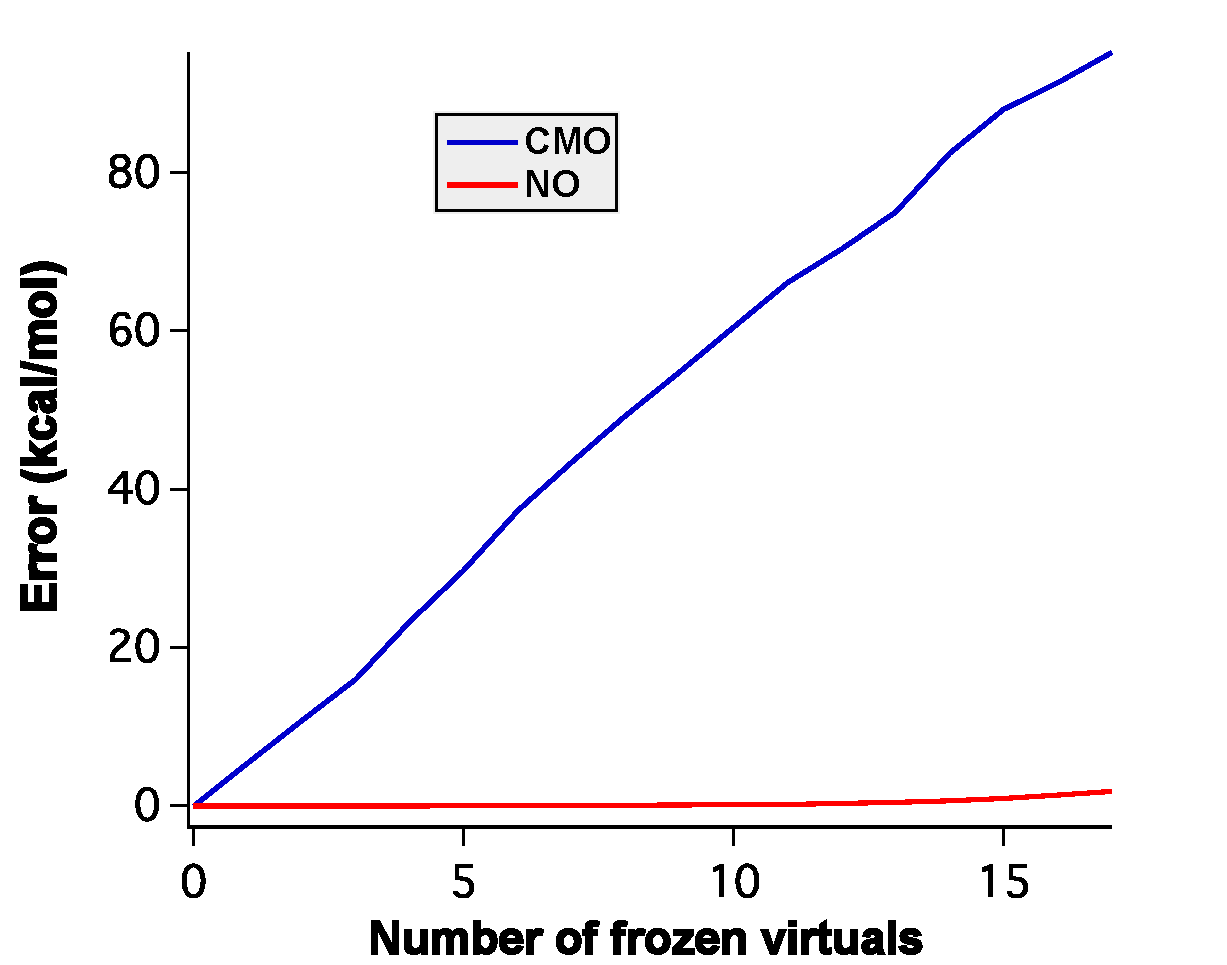
\includegraphics[width=0.7\linewidth]{figures/energy.pdf}
  \caption{Error in the CCSD energy of H$_2$O$_2$ in kcal/mol as a 
           function of the number of frozen virtual orbitals in both CMO and NO bases.} 
  \label{fig:energy}
\end{figure}
%%%%%%%%%%%%%%%%%%%%%%%%%%%%%%%%%%%%%%%%%%%%%%%%%%%%%%%%%%%%%%%
\begin{figure}
  \centering
  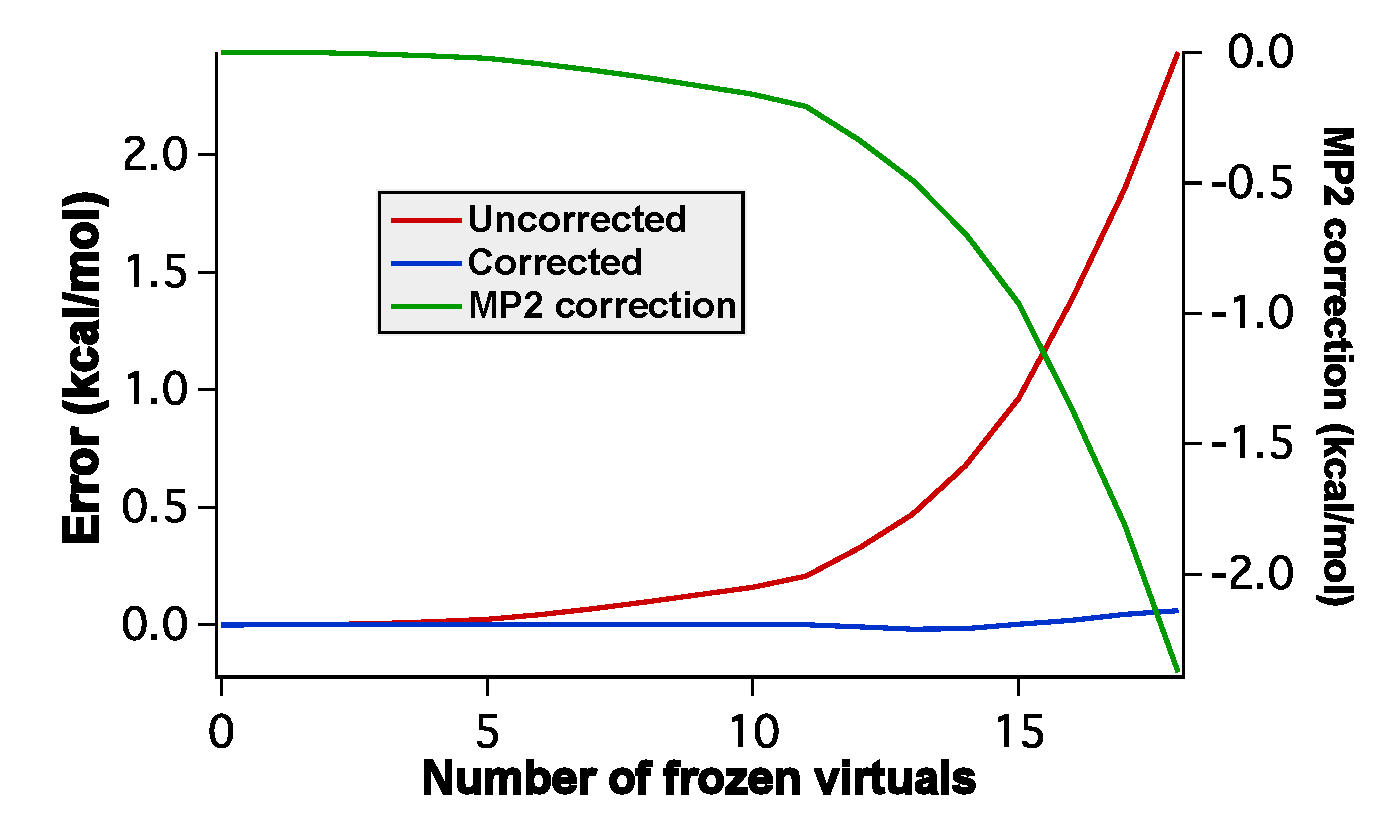
\includegraphics[width=0.7\linewidth]{figures/Mp2c.pdf}
  \caption{Error in CCSD energy of H$_2$O$_2$ in the NO bases, with and without MP2 corrections 
        and MP2 correction as a function of the number of frozen virtual orbitals.}
\label{fig:MP2_corr}
\end{figure}
%%%%%%%%%%%%%%%%%%%%%%%%%%%%%%%%%%%%%%%%%%%%%%%%%%%%%%%%%%%%%%%
\begin{figure}
  \centering
  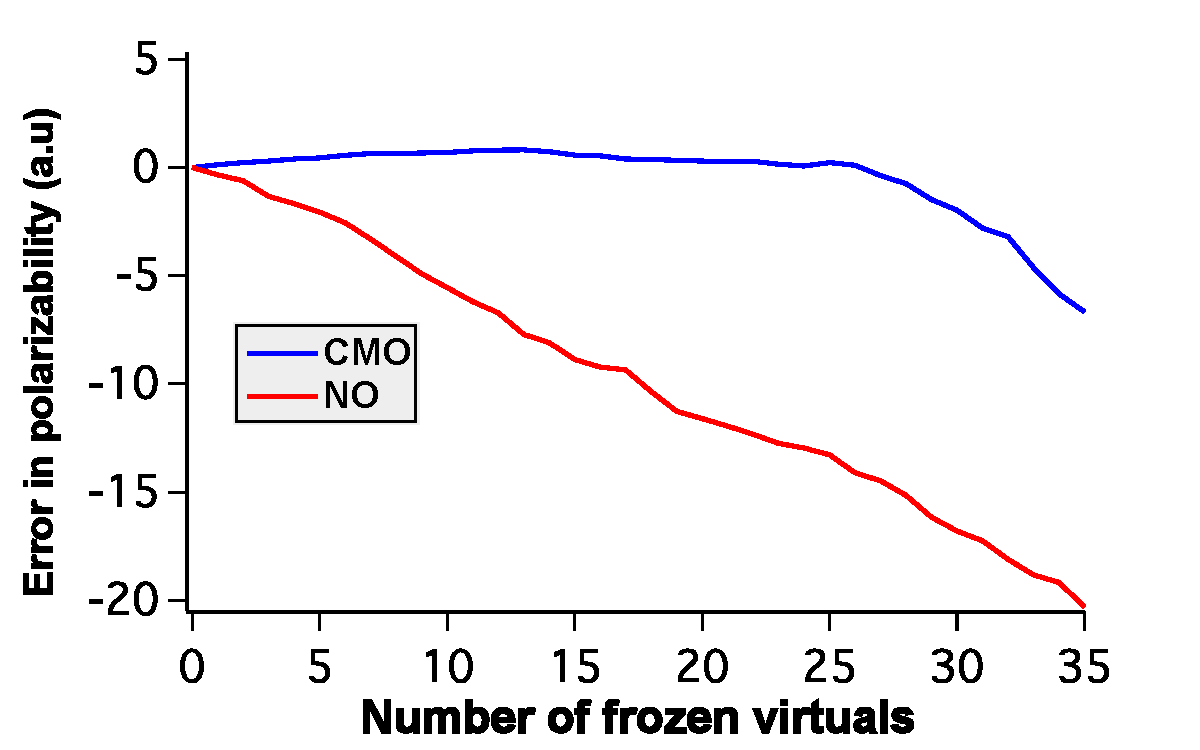
\includegraphics[width=0.6\linewidth]{figures/h2o2_polar.pdf}
  \caption{Errors in the CCSD/aDZ dynamic polarizability (589
nm) of H$_2$O$_2$ in 
       in both CMO and NO bases as a function of number of virtual orbitals removed.}
   \label{fig:polar_h2o2}
\end{figure}
%%%%%%%%%%%%%%%%%%%%%%%%%%%%%%%%%%%%%%%%%%%%%%%%%%%%%%%%%%%%%%%
\begin{figure}
  \centering
  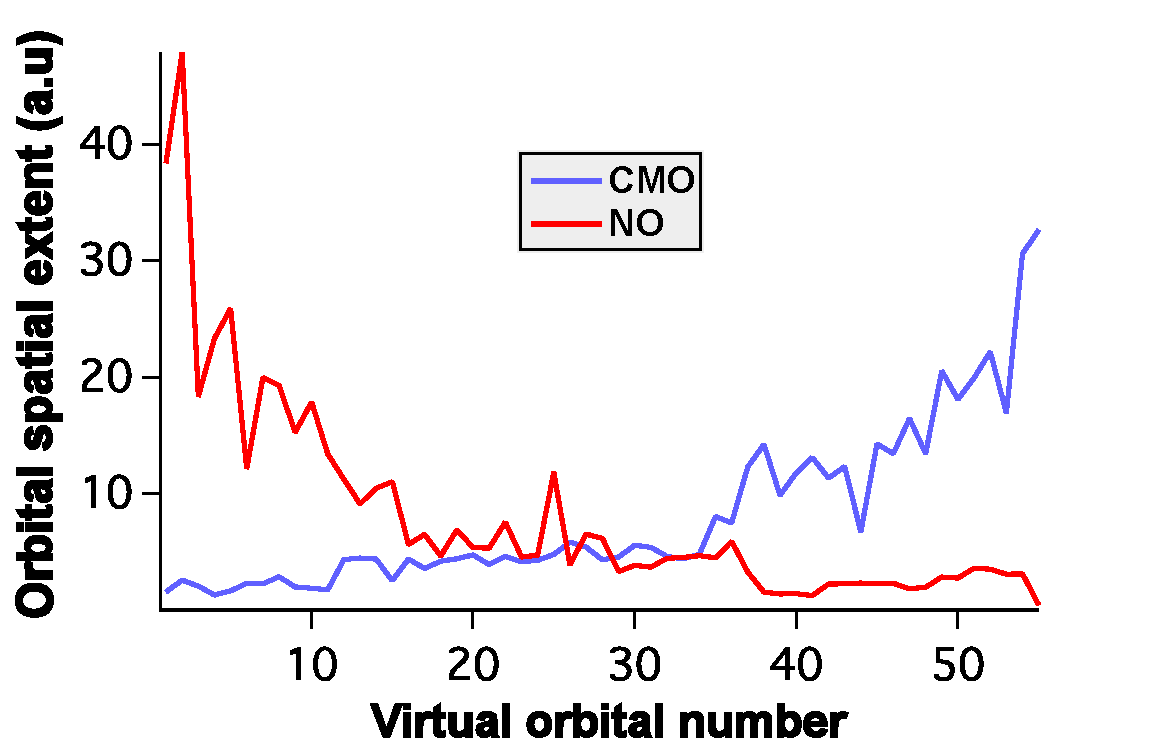
\includegraphics[width=0.6\linewidth]{figures/spatial.pdf}
  \caption{Spatial extent ($\langle r^2\rangle$) of virtual
orbitals of H$_2$O$_2$ in both CMO and NO bases.  Orbitals are ordered
left-to-right by
decreasing energy (CMOs) or increasing occupation number (NOs).}
   \label{fig:spatial}
\end{figure}

%%%%%%%%%%%%%%%%%%%%%%%%%%%%%%%%%%%%%%%%%%%%%%%%%%%%%%%%%%%%%%%
\begin{figure}
  \centering
  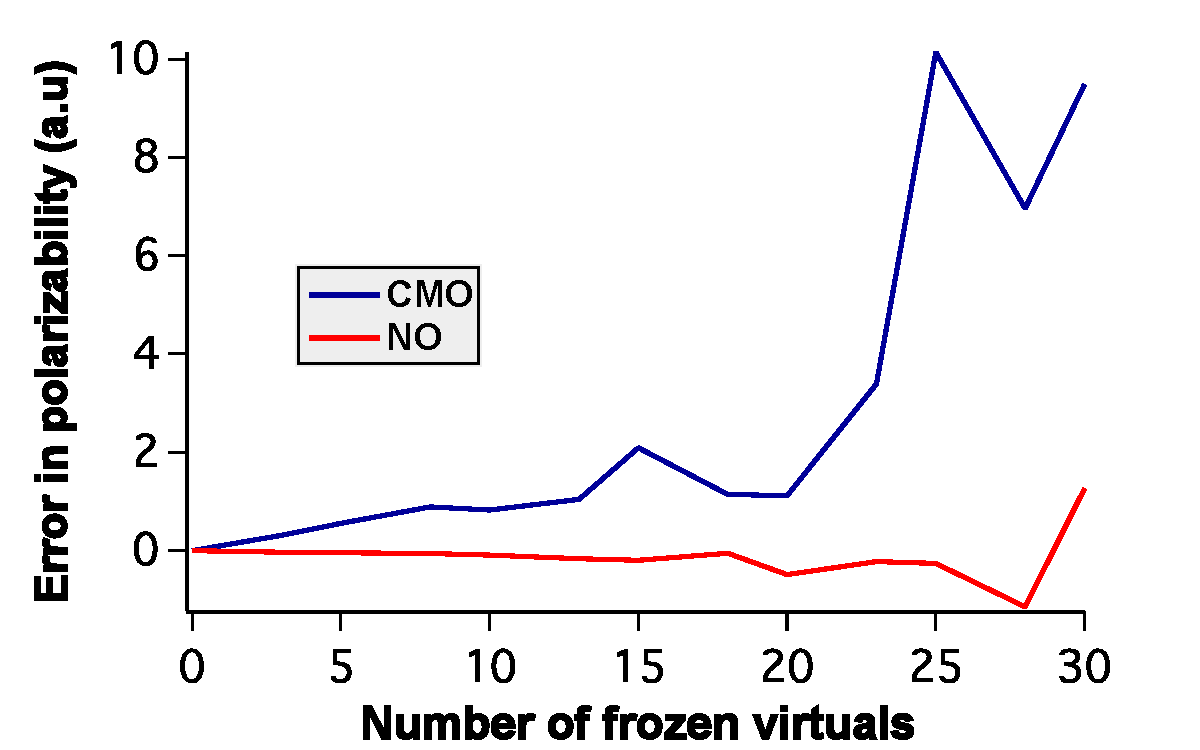
\includegraphics[width=0.6\linewidth]{figures/polar_static.pdf}
  \caption{Errors in the CCSD/aDZ static polarizability 
(including orbital relaxation effects) of H$_2$O$_2$ in
       in both CMO and NO bases as a function of number of virtual orbitals
removed.}
   \label{fig:static}
\end{figure}

%%%%%%%%%%%%%%%%%%%%%%%%%%%%%%%%%%%%%%%%%%%%%%%%%%%%%%%%%%%%%%%
\begin{figure}
  \centering
  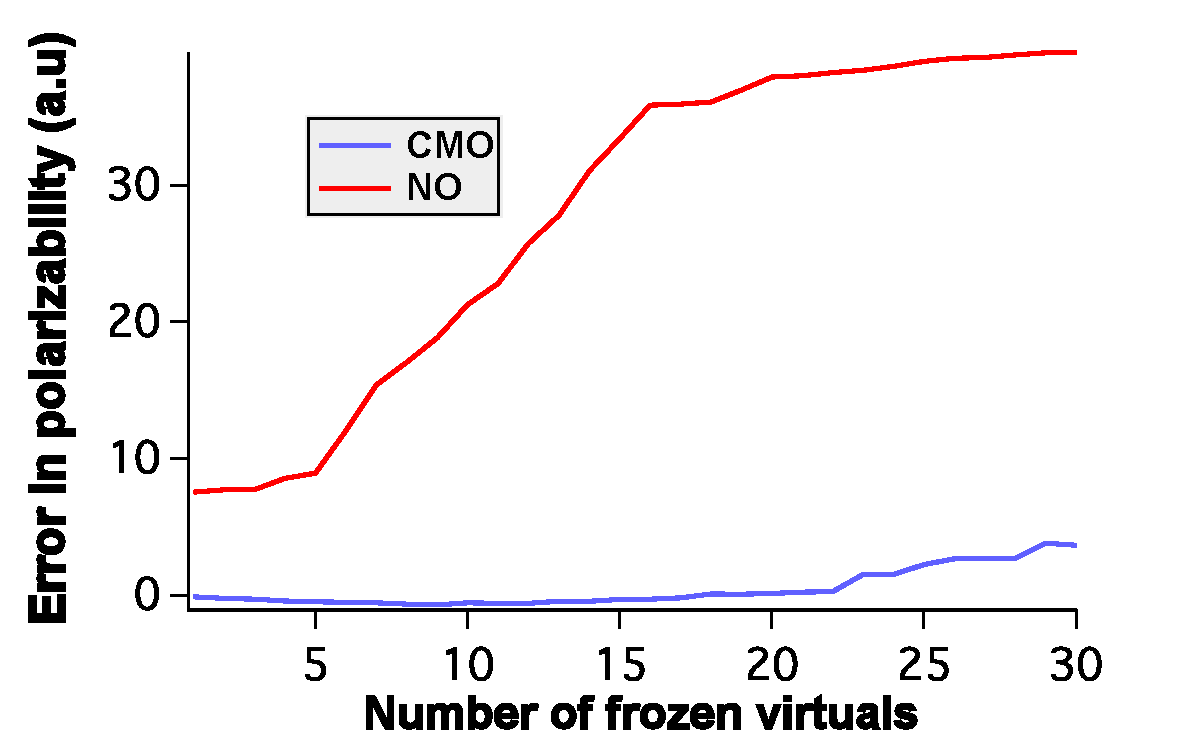
\includegraphics[width=0.6\linewidth]{figures/sort_spatial.pdf}
  \caption{Errors in the CCSD/aDZ dynamic polarizability (589
nm) of H$_2$O$_2$ as a function of the number of virtual CMOs or NOs deleted,
ordered by increasing spatial extent, $\langle r^2 \rangle$.}
   \label{fig:sort_spatial}
\end{figure}
%%%%%%%%%%%%%%%%%%%%%%%%%%%%%%%%%%%%%%%%%%%%%%%%%%%%%%%%%%%%%%%
\begin{figure}
  \centering
  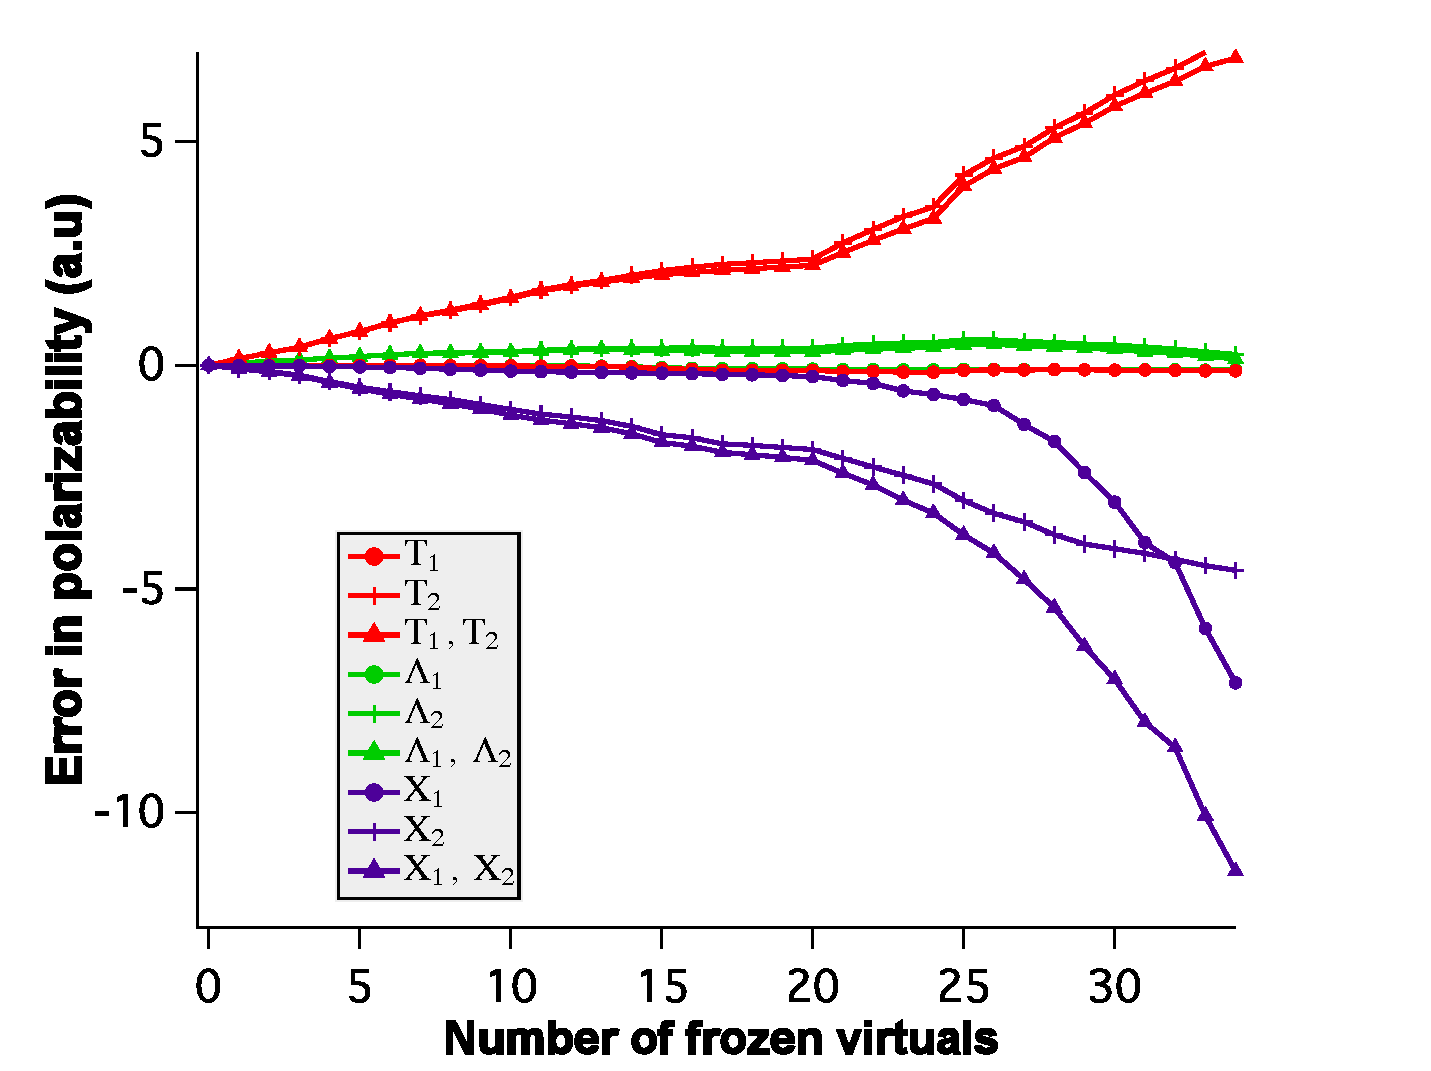
\includegraphics[width=0.6\linewidth]{figures/amp_trunc_cmo.pdf}
  \caption{Errors introduced in CCSD/aDZ polarizabilities of
H$_2$O$_2$ in the virtual CMO bases by the truncation of different classes of wave
function amplitudes.}
   \label{fig:amp_trunc_cmo}
\end{figure}
%%%%%%%%%%%%%%%%%%%%%%%%%%%%%%%%%%%%%%%%%%%%%%%%%%%%%%%%%%%%%%%
\begin{figure}
  \centering
  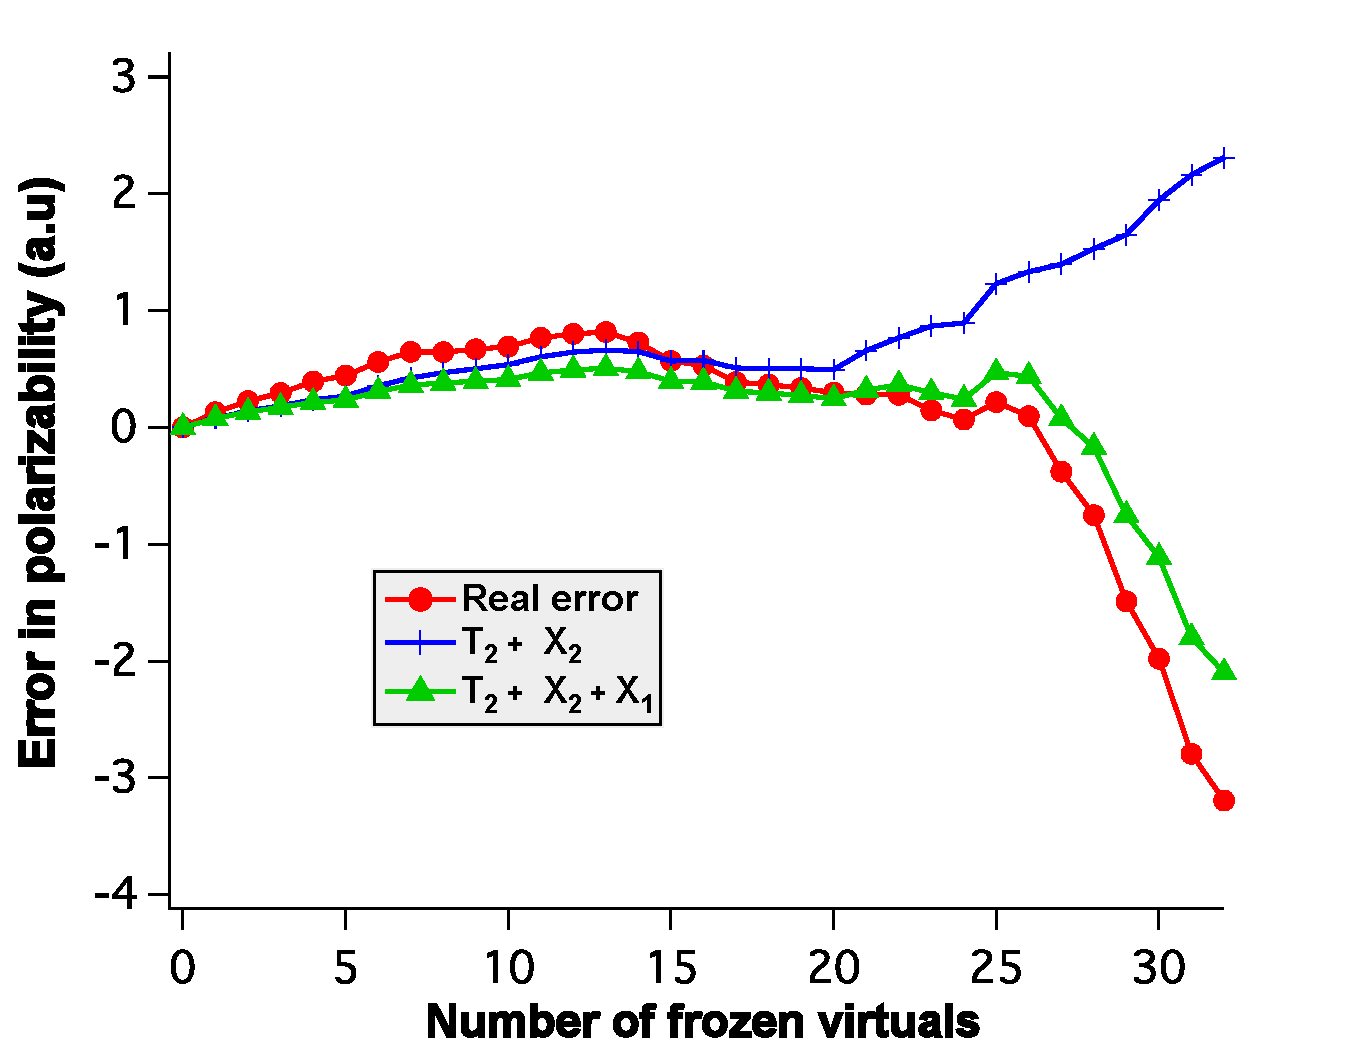
\includegraphics[width=0.6\linewidth]{figures/error_cmpare.pdf}
  \caption{Errors introduced in CCSD/aDZ polarizabilities of
H$_2$O$_2$ in the virtual CMO bases by the truncation of specific classes of wave
function amplitudes as compared to the total errors obtained by freezing of
virtual CMOs.}
   \label{fig:error_compare}
\end{figure}
%%%%%%%%%%%%%%%%%%%%%%%%%%%%%%%%%%%%%%%%%%%%%%%%%%%%%%%%%%%%%%%
\begin{figure}
  \centering
  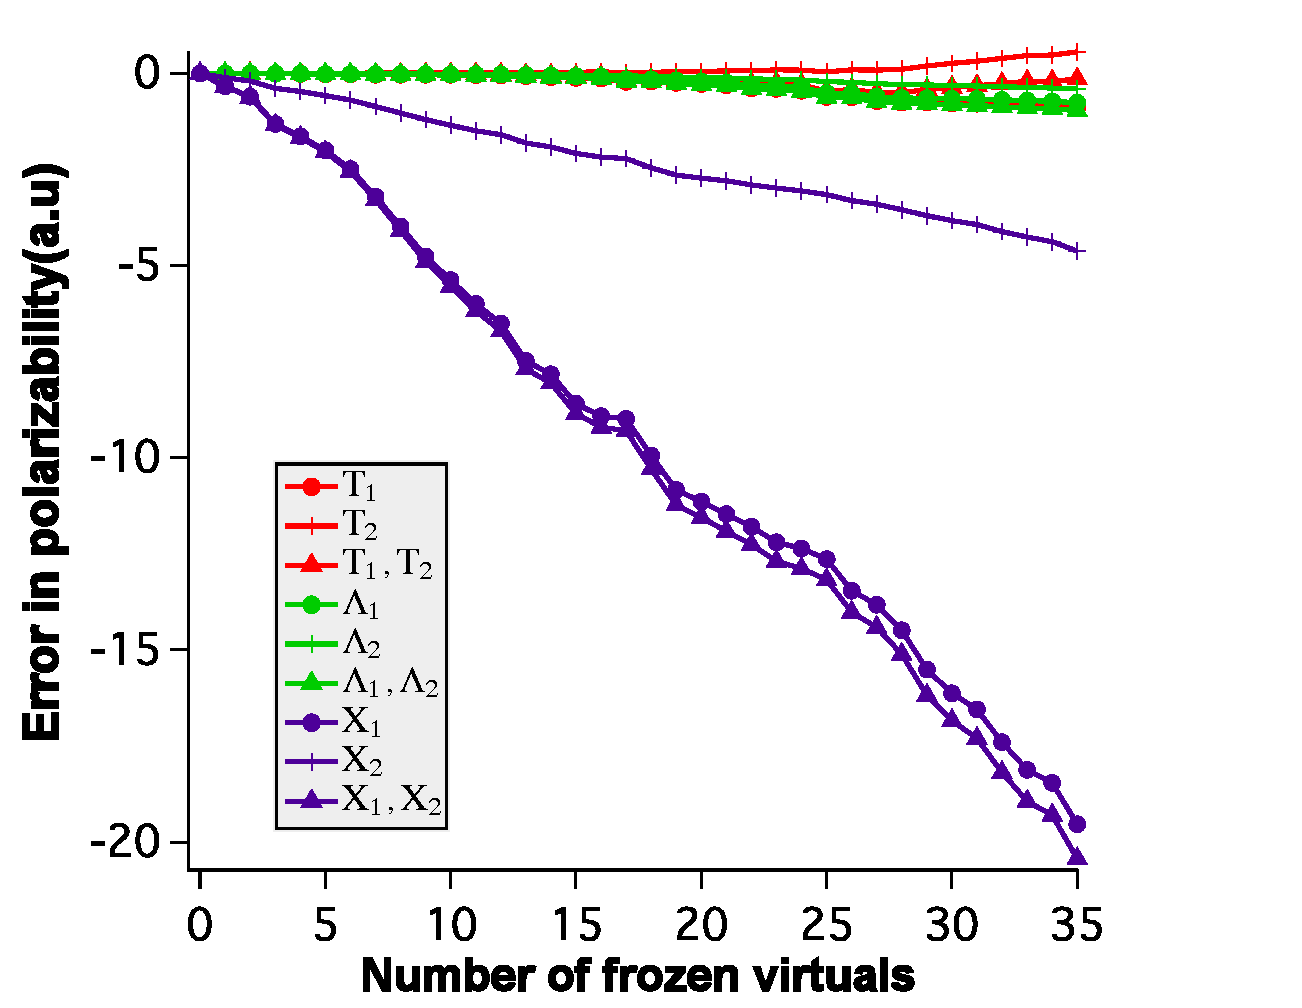
\includegraphics[width=0.6\linewidth]{figures/amp_trunc_no.pdf}
  \caption{Errors introduced in CCSD/aDZ polarizabilities of
H$_2$O$_2$ in the virtual NO bases by the truncation of different classes of wave
function amplitudes.}
   \label{fig:amp_trunc_no}
\end{figure}
%%%%%%%%%%%%%%%%%%%%%%%%%%%%%%%%%%%%%%%%%%%%%%%%%%%%%%%%%%%%%%%
\begin{figure}
  \centering
  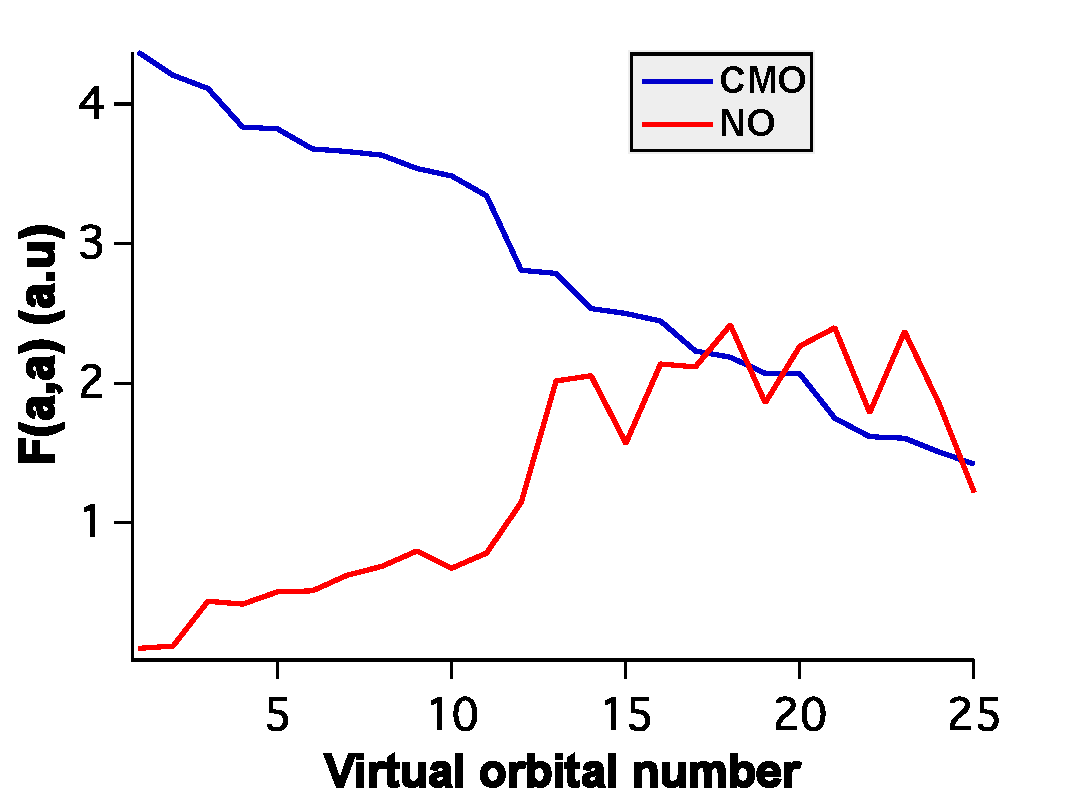
\includegraphics[width=0.6\linewidth]{figures/Faa.pdf}
  \caption{Virtual diagonal elements (a.u.) of the Fock matrix in
the CMO and NO bases.}
   \label{fig:Faa}
\end{figure}
%%%%%%%%%%%%%%%%%%%%%%%%%%%%%%%%%%%%%%%%%%%%%%%%%%%%%%%%%%%%%%%
\begin{figure}
  \centering
  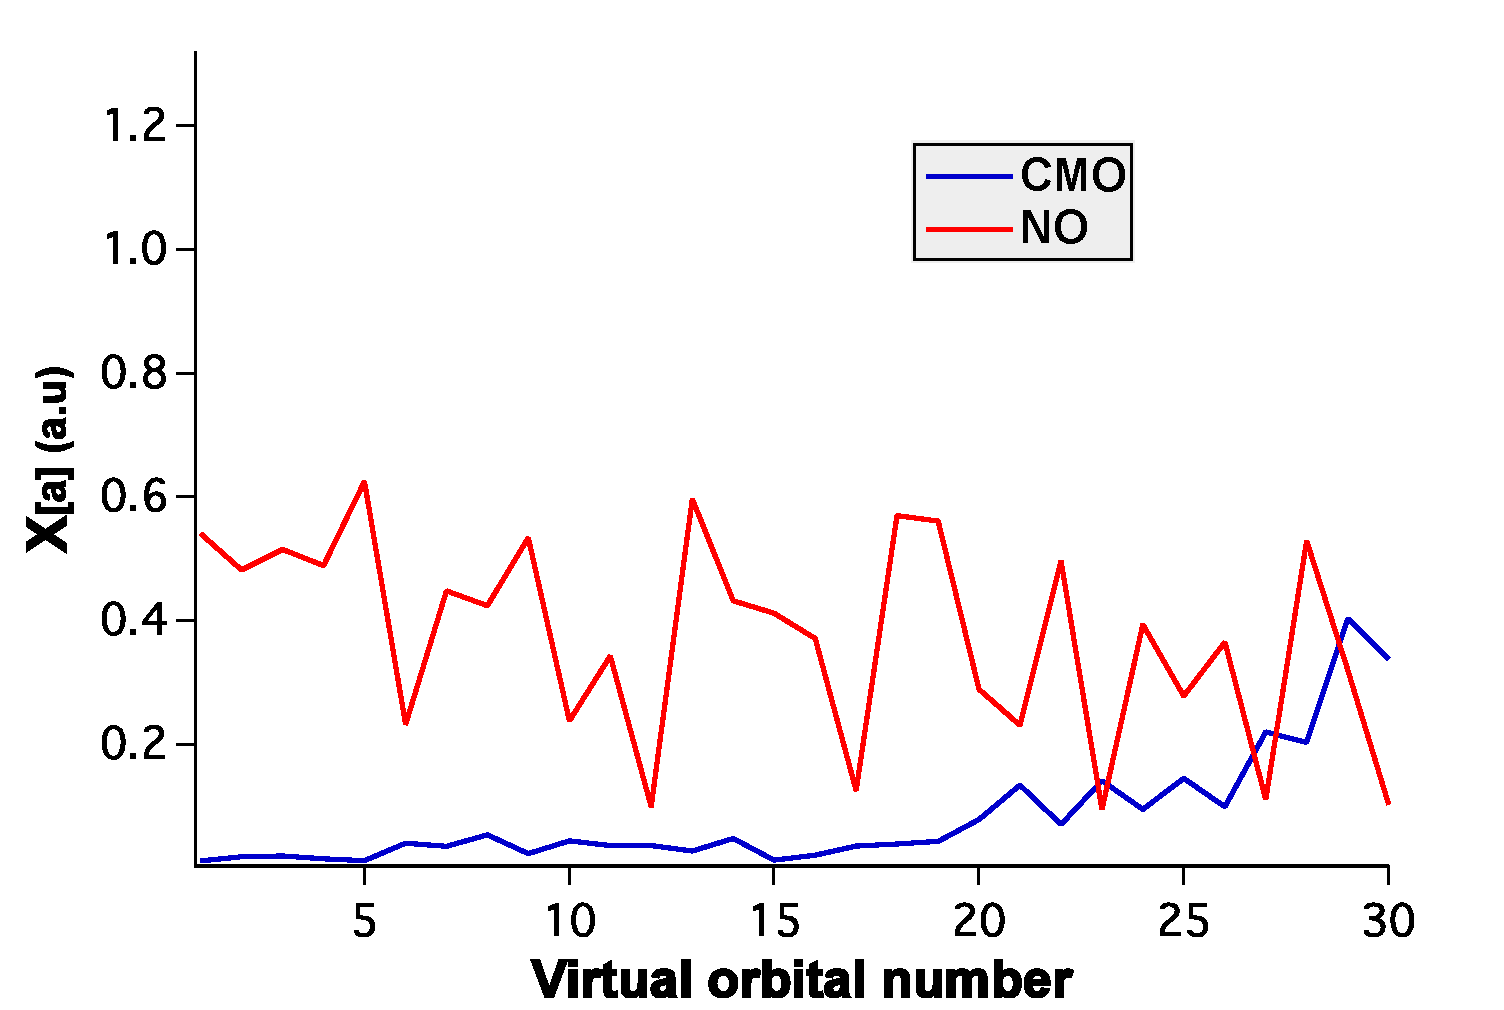
\includegraphics[width=0.6\linewidth]{figures/X1.pdf}
  \caption{Sum of the absolute values of $\hat{X}_1$
amplitudes for a given virtual, $\sum_i \left|X_i^a\right|$, for perturbation $\mu_x$
and frequency 589 nm, plotted for each virtual NO or CMO.}
   \label{fig:X1}
\end{figure}
%%%%%%%%%%%%%%%%%%%%%%%%%%%%%%%%%%%%%%%%%%%%%%%%%%%%%%%%%%%%%%%
\begin{figure}
  \centering
  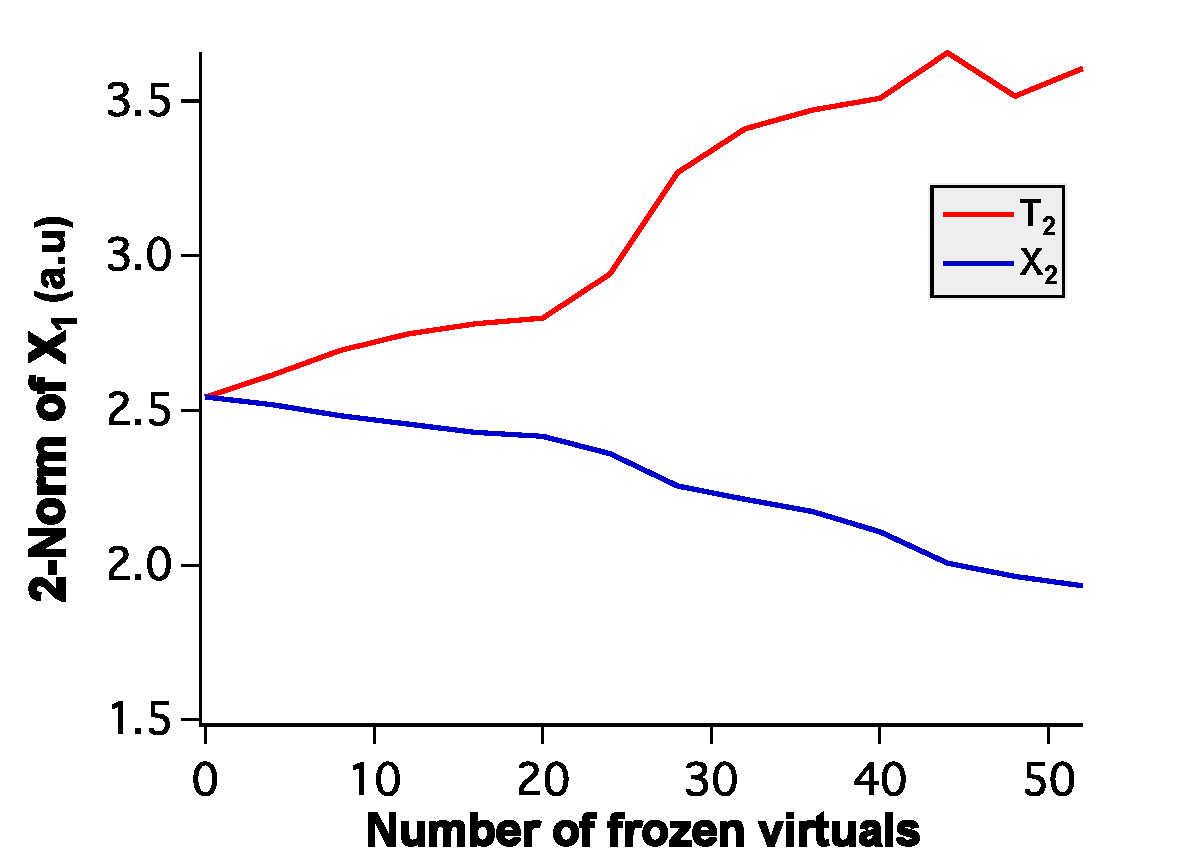
\includegraphics[width=0.6\linewidth]{figures/norm.pdf}
  \caption{The 2-norm of the $\hat{X}_1$ amplitude vector in
the CMO bases as a function of the truncation of classes of unperturbed 
$\hat{T}_2$ and perturbed $\hat{X}_2$ amplitudes.}
   \label{fig:norm}
\end{figure}
%%%%%%%%%%%%%%%%%%%%%%%%%%%%%%%%%%%%%%%%%%%%%%%%%%%%%%%%%%%%%%%
%\begin{figure}
%  \centering
%  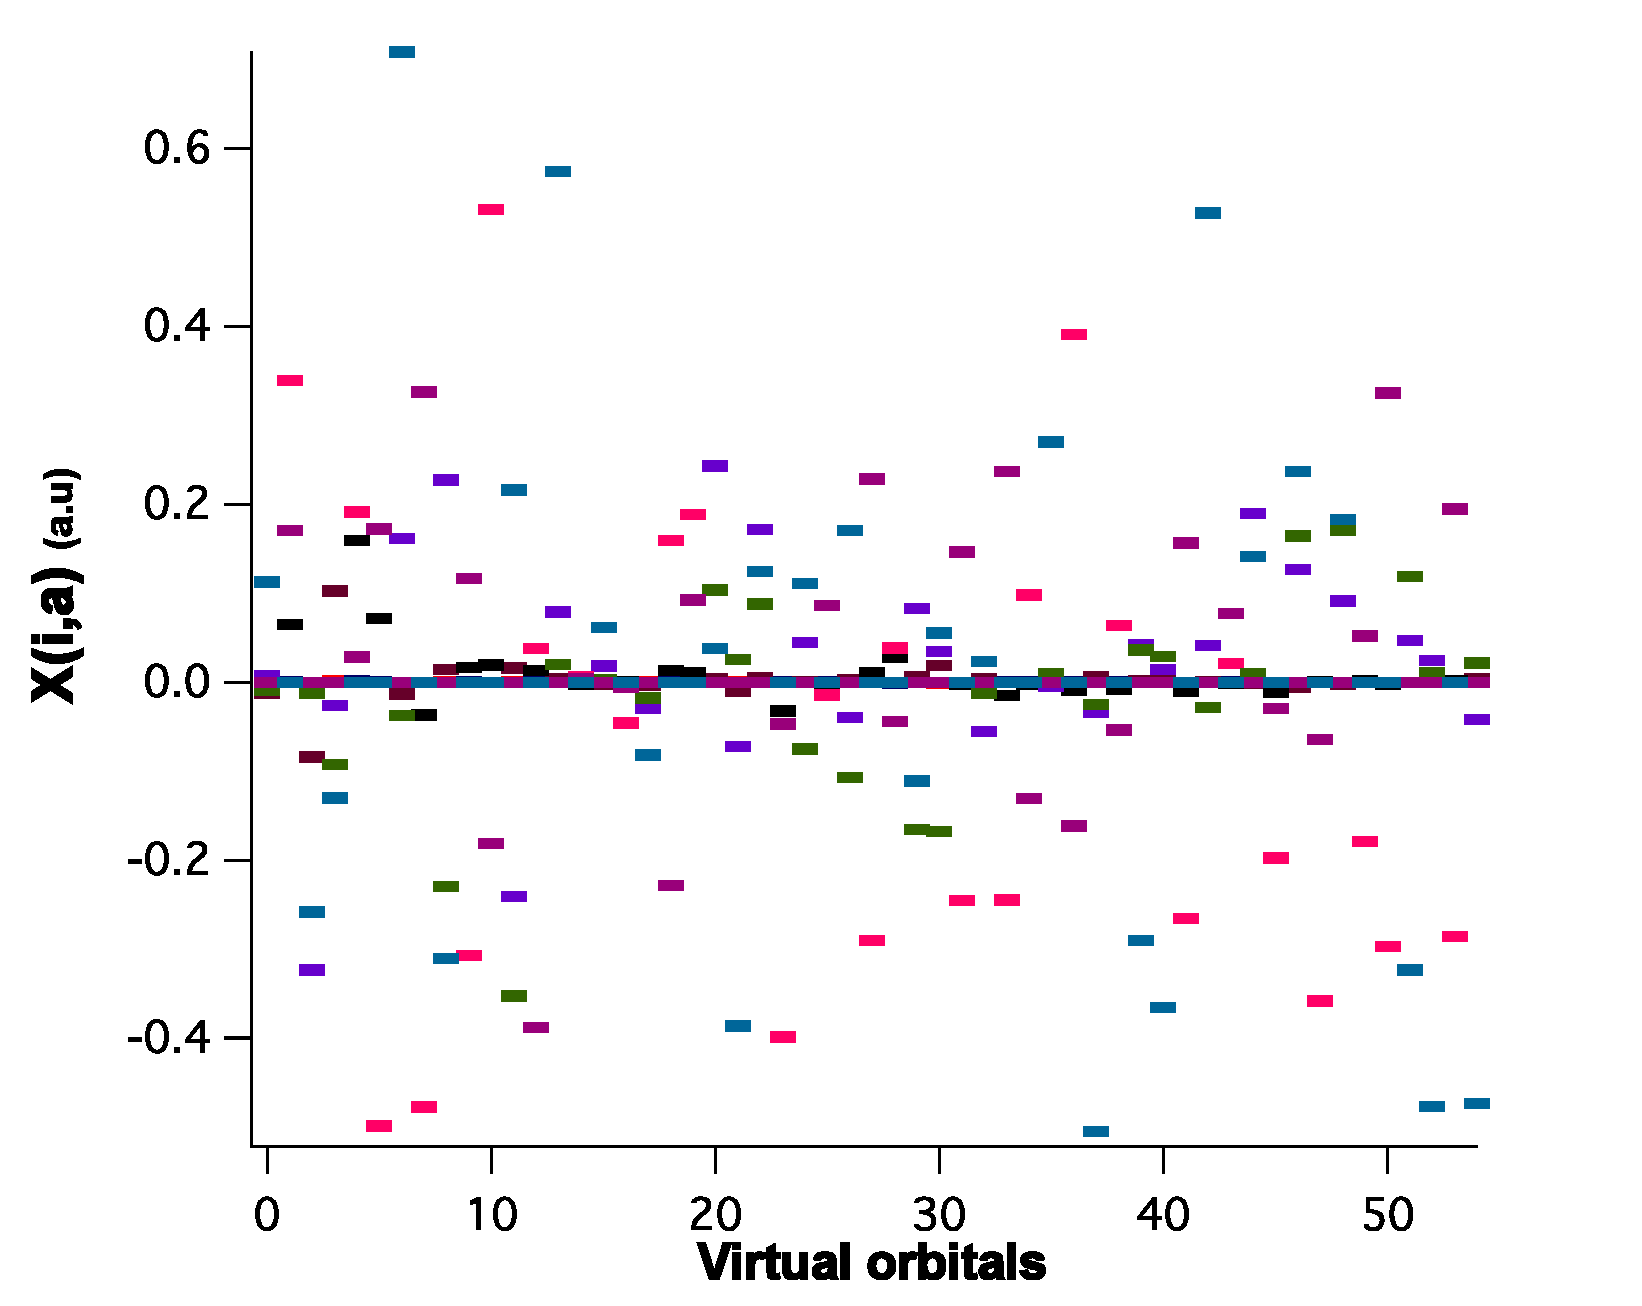
\includegraphics[width=0.6\linewidth]{figures/X1_no.pdf}
%  \caption{\footnotesize{$X_1$ amplitudes $X^{\mu_x}_{ia}$(589 nm) in the NO basis. For each virtual orbital there are nine virtual-occupied pairs.}}
%   \label{fig:X1_no}
%\end{figure}
%%%%%%%%%%%%%%%%%%%%%%%%%%%%%%%%%%%%%%%%%%%%%%%%%%%%%%%%%%%%%%%
\begin{figure}
  \centering
  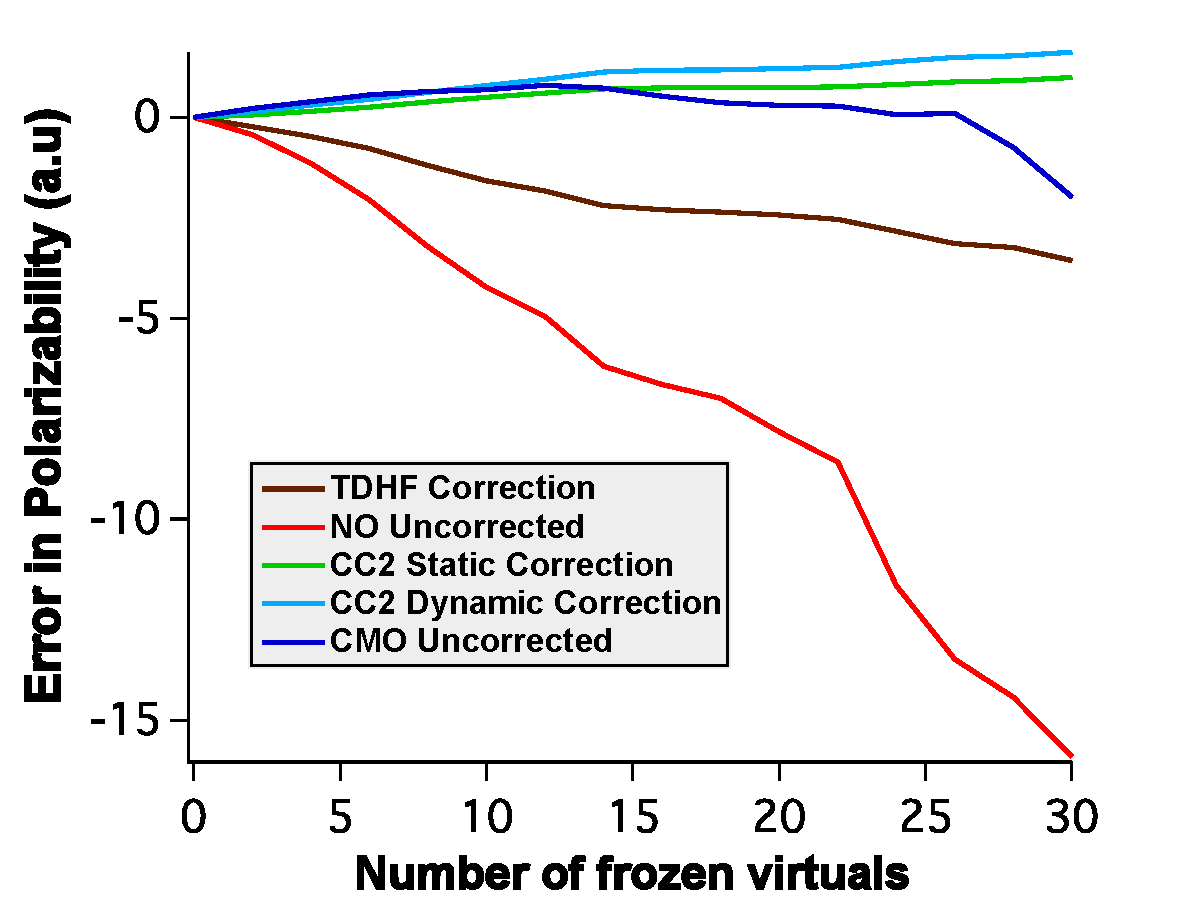
\includegraphics[width=0.6\linewidth]{figures/correctn.pdf}
  \caption{Correction schemes for the external truncated
NO space for the CCSD/aDZ polarizabilities of H$_2$O$_2$.}
   \label{fig:corrections}
\end{figure}
%%%%%%%%%%%%%%%%%%%%%%%%%%%%%%%%%%%%%%%%%%%%%%%%%%%%%%%%%%%%%%%

\begin{figure}
  \centering
  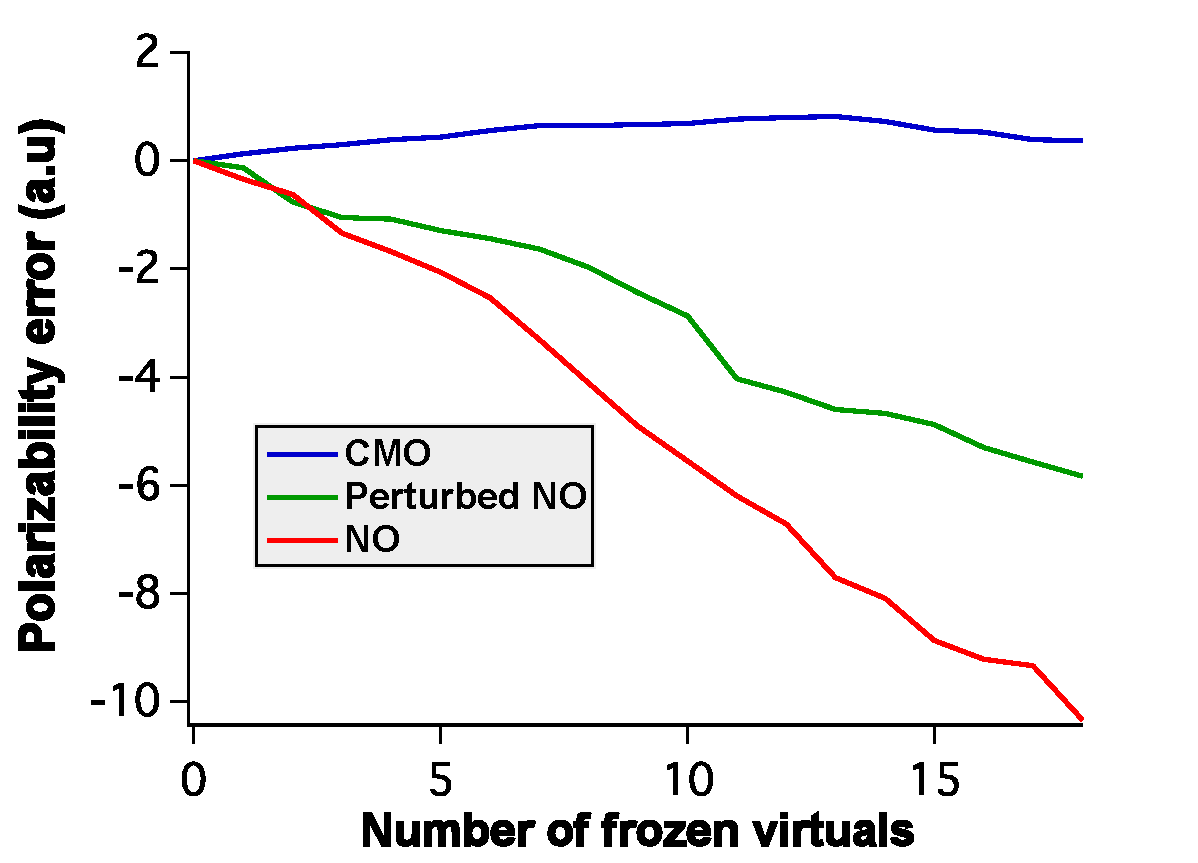
\includegraphics[width=0.6\linewidth]{figures/perturbed.pdf}
  \caption{Errors introduced in CCSD/aDZ polarizabilities of
H$_2$O$_2$ in the virtual CMO and NO bases, as well as the perturbed
virtual NO basis as a function of number of virtual orbitals removed.}
   \label{fig:perturb}
\end{figure}
%%%%%%%%%%%%%%%%%%%%%%%%%%%%%%%%%%%%%%%%%%%%%%%%%%%%%%%%%%%%%%%
\begin{figure}
  \centering
  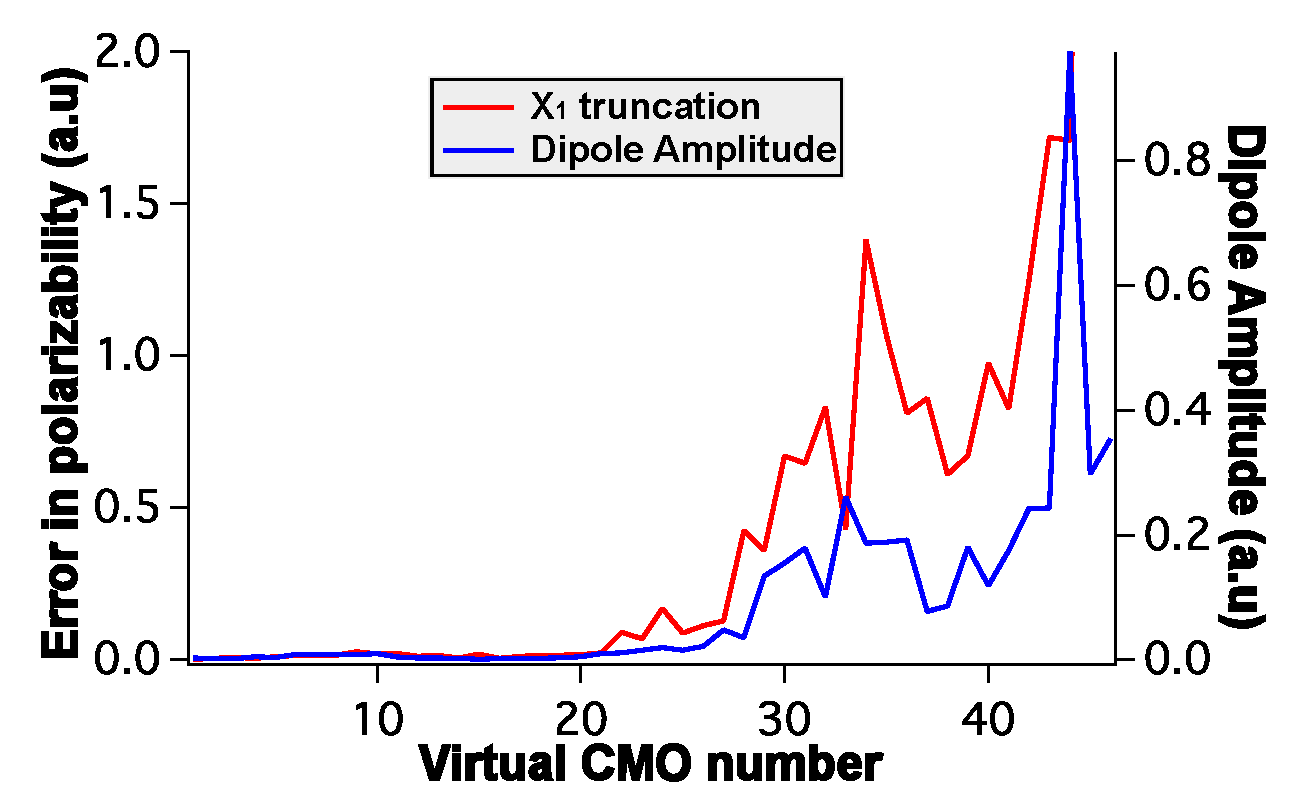
\includegraphics[width=0.6\linewidth]{figures/diplength.pdf}
  \caption{Absolute errors introduced in CCSD/aDZ
  polarizabilities of H$_2$O$_2$ due to truncation of $\hat{X}_1$ amplitudes and
  dipole amplitudes plotted as a function of different virtual CMOs.}
   \label{fig:dipole_length}
\end{figure}
%%%%%%%%%%%%%%%%%%%%%%%%%%%%%%%%%%%%%%%%%%%%%%%%%%%%%%%%%%%%%%%


\newpage
\begin{center}
{\bf TOC Graphic}
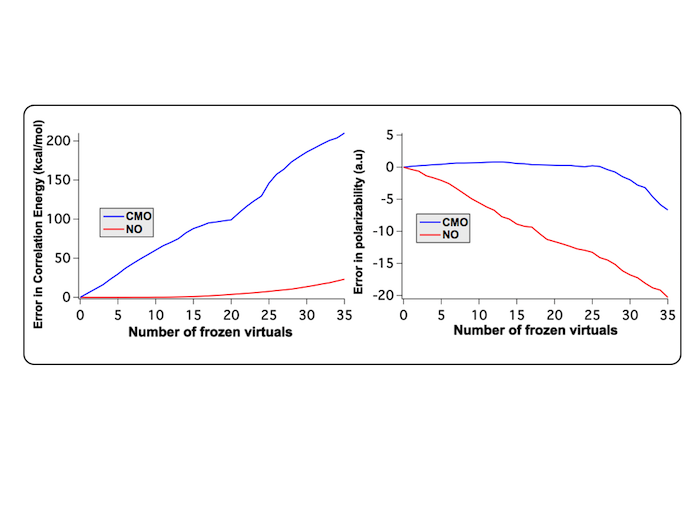
\includegraphics[width=1.0\linewidth]{figures/toc.png}
\end{center}

%
%\end{document}

\chapter{Perturbed Pair Natural Orbitals for Coupled-Cluster Linear-Response\\Theory}
\markright{Ashutosh Kumar \hfill Chapter 5. Perturbed Pair Natural Orbitals\hfill}
%\documentclass[journal=jpccck,manuscript=article]{achemso}
%\usepackage[numbers,super]{natbib}
%
%\usepackage{graphicx}
%\usepackage{xcolor}
%\usepackage{todonotes}
%
%\def\ket#1{| #1 \rangle}
%\def\bra#1{\langle #1 |}
%
%\usepackage[utf8]{inputenc} % set input encoding (not needed with XeLaTeX)
%\usepackage{verbatim}
%\usepackage{amsfonts}
%\usepackage{graphicx}
%\newcommand{\overbar}[1]{\mkern 2.2mu\overline{\mkern-2.2mu#1\mkern-2.2mu}\mkern 2.2mu}
%\usepackage{multirow}
%\usepackage{array}
%\usepackage{varwidth}
%\usepackage{bm}
%
%\title{Pair Natural Orbitals ++ approach for Coupled Cluster Linear-Response Theory}
%\author{Ashutosh Kumar}
%\affiliation{Department of Chemistry, Virginia Tech, Blacksburg, Virginia 24061, U.S.A.}
%\author{T.\ Daniel Crawford}
%\email{crawdad@vt.edu}
%\affiliation{Department of Chemistry, Virginia Tech, Blacksburg, Virginia 24061, U.S.A.}
%
%\date{\today}
%
%\begin{document}
%
%\begin{abstract} We present here the the modified  pair natural-orbital (NO) 
%approach, which we call PNO++ for a compact representation of the 
%response of the coupled cluster wavefunction to external electric
%and magnectic fields. In our earlier work,%\cite{McAlexander15}
%we showed that the regular PNO method performs rather poorly for 
%%The frozen-virtual natural-orbital (NO) approach, whereby the
%%unoccupied-orbital space is constructed using a correlated density such as
%%that from many-body perturbation theory, has proven to yield compact wave
%%functions for determining ground-state correlation energies and associated
%%properties, with corresponding occupation numbers providing a guide to the
%%truncation of the virtual space.  In this work this approach is tested for the
%%first time for the calculation of higher-order response properties,
%%particularly frequency-dependent dipole polarizabilities using coupled-cluster
%%theory.  We find that such properties are much more sensitive to the
%%truncation of virtual space in the natural orbital (NO) basis than in the
%%original canonical molecular orbital (CMO) basis, with truncation errors
%%increasing linearly with respect to the number of frozen virtual NOs.  The
%%reasons behind this poor performance include the more diffuse nature of NOs
%%with low occupation numbers as well as the reduction in sparsity of the
%%perturbed singles amplitudes in the NO basis and the neglect of orbital
%%response.  We tested a number of approaches
%%to improve the performance of the NO space, including the use of a
%%field-perturbed density to define the virtual orbitals and various
%%external-space corrections.  The truncation of the CMO space, on the other
%%hand, yields errors in coupled-cluster dipole polarizabilities of less than
%%2\% even after removing as much as 50\% of the full virtual space. We find
%%that this positive performance of the CMO space results from a cancellation of
%%errors due to the truncation of the unperturbed and perturbed amplitudes, as
%%well as sparsity of the singles amplitudes.  We introduce a simple criterion
%%called a dipole amplitude to use as a threshold for truncating the CMO basis
%%for such property calculations.  \end{abstract}
%\end{abstract}
%\maketitle

\section{Introduction}
Accurate {\em ab initio} models like the coupled cluster theory have been 
used quite reliably to predict the chiroptical properties of molecules\cite{}
However, they have been limited to very small system sizes due to the heavy 
computational expenses associated with such methods. For example, the coupled cluster 
singles and doubles method (CCSD) has a high polynomial scaling of $O(N^6)$, where
N is some measure of the system size. This is clearly unphysical as the phenomenon 
of dynamic electron-correlation, which these methods aim to capture, is local in nature.\cite{}
This steep scaling can be attributed to the use of delocalized canonical 
Hartree-Fock MOs (CMOs) as the one electron basis for representing the wavefunction. 
Local correlation techniques try to exploit the intrinsic sparsity in correlated wavefunctions  
by unitarily localizing the occupied orbitals (LMOs) using methods like Boys-Foster, Pipek-Mezey etc\cite{}.
and constructing excitation domains corresponding to each LMO. The sizes of these domains
are usually very small compared to the full virtual space and become constant in the asymptotic limit,
making these approaches reduced-scaling. Saebo and Pulay's introduction of projected atomic orbitals (PAO)
as a representation of the virtual space stands as one of the earliest works in this regard\cite{}. As the name
suggests, PAOs are formed by projecting out the occupied MO components from the AO basis. Since the PAOs are
centered on atoms (just like AOs), an excitation domain for a given LMO can be constructed by 
including only those PAOs which are on or near the atoms associated with that LMO. Subsequently, domains 
corresponding to a pair of LMOs can be formed by taking a union of the PAO space of both the LMOs and so on.
Wener, Sch{\"u}tz and co-workers \cite{} were the first to apply these concepts within the framework of CC theory.
By employing truncated PAO domains coupled with other approximations like weak and distant pairs, they were 
able to achieve linear scaling while maintaining accurate description of ground-state properties
like reaction enthalpies, thermodynamic constants etc.\cite{} However, extension of such 
approaches to excited states to calculate properties like excitation energies has seen 
limited success as the domain size requirements for describing both ground and excited 
states accurately have been shown to be quite large.\cite{} This is unsurprising as 
excitations in say a charge-transfer excited state could be fairly non-local. PAOs have also been 
used within the context of CC linear response theory to calculate higher-order response 
properties like (hyper)polarizabilities, chiroptical response etc. albeit on a 
much smaller scale.\cite{} In 2004, Korona and Werner\cite{} used PAOs with local 
coupled cluster singles and doubles method (LCCSD) to calculate electric dipole moments and 
static polarizabilities where they got average errors of 1.61\% and 0.48\% respectively.
Further minimization of the errors required building bigger domains leading to a 
significant increase in computational expenses. In the same year, Russ and Crawford\cite{}
used a modified domain building procedure within the PAO framework, where they augmented 
the ground state orbital domains on the basis of first-order orbital response coefficients 
obtained by sloving the coupled-perturbed Hartree-Fock equations, to calculate CC static polarizabilities. 
A few years later, they extended this formalism to calculate dynamic polarizabilities and optical rotations\cite{}. 
While the localization errors for linear molecular structures were shown to be only a few percent of canonical
results, three dimensional compounds required significantly large domains, specially for 
optical rotations. A similar conclusion was drawn when Friedrich and co-workers
applied the incremental scheme, a fragmentation based local correlation 
technique to calculate CC dynamic polarizabilities.\cite{} 
For a more detailed overview of the applications of PAO based methods in this field, 
please refer to ref\cite{McAlexander15}. Within the framework of local correlation,
the pair natural orbitals (PNOs) introduced in 1970s by Edimnston and Krauss\cite{}, 
Meyer\cite{}, Ahlrichs\cite{}, Kutzelnigg\cite{}, Staemmler and co-workers\cite{} 
and orbital specific virtuals (OSVs) developed by Chan and co-workers in 2011 \cite{}, are 
are other popular alternatives to PAOs for a compact representation of the
virtual space. In the PNO approach, each pair of LMOs have their own virtual space 
which can be obtained by the diagonalization of the virtual-virtual 
block of an approximate 1-electron pair specific density. The OSV approach
on the other hand involves diagonalization of a separate density for each LMO.
Although the PNOs could compress the 


 

initially abandoned due to the comptational costs involved in the transfoirmation 

% PNOs are other popular correlation techniques.
% introduced as pseudonatural orbitals  by ...
% each pair of LMO has its own virtual space
% obtained from diagonalization of an approximate pair
% density. but abandoned due to transformation of teis to pno basis
% Neese and co-wokers revived by DF mechanisms
% much more compact than PAO.
% PAO scheme to help in integral transformations further,
% thus PAO + PNO -> DL-PNO-CCSD(T) calculations on proteins -> very succesfull
% excited states very successful - hattig, valeev, excitation energies.

% how about response properties
% only McAlexander and co-workers
% showed that PNO much more compact than PAO and OSV approach developed by chan and co-workers
% However, rotations for 2-d and 3-d systems very sensitive to truncation
% inspired by our earlier work with natural orbitals,
% want to improve that usiing field perturbed densities 
%
% Here we explotre just that!!!! 


\section{Response Theory}
\section{Pair Natural Orbitals}
\section{Computational Details}
\section{Results and Discussions}
\section{Conclusions}




%The most popular approaches
%of inducing sparsity in the virtual orbital space 
%are based on the concept of Natural
%orbitals (NOs), introduced by L{\"o}wdin in 1955\cite{}as the eigenvectors of  
%the one electron reduced density matrices (1-RDMs), where he referred to 
%the corresponding eigenvalues as occupation numbers (ONs). L{\"o}wdin showed  
%the configuration interaction (CI) wavefunction expansion in the NO basis 
%converges quite rapidly compared to the CMO basis. Motivated by L{\"o}wdin's 
%findings, Bender, Barr and Davidson\cite{} used NOs obtained from 
%
%a few years later used approximate NOs 
%to construct optimized configurations in their CI calculations on first-row diatomic 
%hydrides. A Barr 
%and Davidson\cite{} employed what they called the frozen form of NOs 
%obtained by diagonalizing only the virtual-virtual block of the density 
%matrix to analyze the nature of the CI method through correlation energy 
%studies on Ne atom; Edminston and Krauss,\cite{}Meyer\cite{}, Ahlrichs and 
%co-workers\cite{} developed the concept of pair natural orbitals (PNOs) or 
%``pseudonatural orbitals" as the eigenvectors of the 1-RDM associated 
%with a single electron pair. 
%The ONs can be seen as a metric for estimating the importance of a virtual NO in describing
%electron correlation effects and hence all those virtual NOs which have ONs below a given threshold
%can be removed without causing any significant errors in correlation energies. 

%f. Recent work of FVNO and then PNO for excitation energies
%g. How about response properties?
%h. Properties are tough, cite all our papers, harley's paper, 
%Extension of harley's work, can the results be improved by making use of perturbed densities
%, cite my FVNO++ paper and explain the logic behind that
%  but that's only a reduced-prefactor method! how to make it reduced-scaling?
%i. Here we compare the performance of this approach for dynamic polarizabilities and specific 
%   rotations vs regular PNO approach.


%In the construction of many-body electronic wave functions, the scaling of a
%given method with the number of molecular orbitals (MOs) plays a pivotal role
%in the ultimate cost of the calculation.  For many-body methods such as
%coupled cluster (CC),\cite{Shavitt09,Gauss98,Crawford00:review} which, in its
%canonical formulation, displays a higher-order polynomial dependence on the
%number of MOs, numerous mechanisms have been explored over the last half
%century for reducing the size of the virtual-MO space.  Among the earliest of
%these was L{\"o}wdin's\cite{Lowdin55} introduction in 1955 of the concept of
%``natural orbitals'' (NOs) --- orbitals for which the one-electron density
%matrix is diagonal.  L\"owdin demonstrated that NOs yield faster convergence
%of the configuration interaction (CI) wave function expansion than Hartree-Fock MOs.  Some years later,
%Bender and Davidson\cite{Bender69} used natural orbitals in conjunction with
%CI (NO-CI) calculations to construct and analyze the most important
%configurations contributing to the correlated wave functions for a series of
%closed- and open-shell first-row diatomic hydrides.  This work motivated Barr
%and Davidson a year later\cite{Barr70} to utilize only the virtual natural
%orbitals, obtained by diagonalization of the virtual-virtual block of
%the one-electron density matrix, for NO-CI calculations on the Ne atom.
%
%The concept of pair natural orbitals (PNOs -- originally called
%``pseudonatural orbitals'') was developed by Edmiston and
%Krauss,\cite{Edmiston66} by Meyer\cite{Meyer73}, and by Ahlrichs and
%co-workers.\cite{Ahlrichs75} In the PNO approach, the virtual-virtual MO block
%of the one-electron density is constructed and diagonalized independently for
%each occupied MO pair, leading to separate non-orthogonal virtual spaces.
%Although this approach leads to rapid convergence of the correlation energy
%with respect to the size of the virtual space, it was little used following
%initial investigations until it was resurrected in recent years by Neese and
%co-workers with great success in the context of reduced-scaling electron
%correlation methods.\cite{Neese09,Riplinger16}
%
%Following these pioneering efforts, NOs have been exploited in numerous
%applications to construct compact CI,\cite{Fermann94,Sherrill98:CI,Abrams04}
%multiconfigurational self-consistent-field (MCSCF),\cite{Jensen88} and CC wave
%functions.\cite{Sosa89,Taube05,Taube08,Landau10,DePrince13:FNOs,DePrince13} In
%many of these studies, the virtual-MO block of the one-electron density is
%first obtained from a simpler model, such as second-order many-body
%perturbation theory (MBPT) calculation, and then diagonalized to yield the
%virtual-NO space.  The space is then truncated based on an
%occupation-number-related criterion and fixed for the subsequent
%correlated-wave-function calculation.  In addition, the final energy is
%commonly corrected using the second-order M\o ller-Plesset perturbation theory
%(MP2) correlation energy contributions arising from the external virtual
%space.  These studies have indicated that, for energetics and related
%properties, even aggressive truncation of the virtual-NO space often has only
%a small impact on the resulting property as compared to full-space
%computations.  For example, Landau {\em et al.}\cite{Landau10} found that,
%for NOs
%combined with the equation-of-motion coupled-cluster method for ionized states
%(EOM-IP-CC), reduction of the virtual space by up to 70\% yielded truncation
%errors within ca.\ 1 kcal/mol for ionization energies of organic compounds and
%non-parallelity errors in potential surfaces of weakly bound complexes.
%
%While the above studies have demonstrated clearly the usefulness of NOs for
%aggressively truncating the virtual space when computing correlation energies,
%more complex properties have yet to be considered.  As shown in a number of
%recent
%reports,\cite{Korona04,Russ04,Russ08,McAlexander12,Friedrich15,McAlexander15:LRCC}
%properties that are related to the linear- or higher-order response of the
%wave function to external electric and magnetic fields, for example, exhibit
%much greater sensitivity to the quality of the wave function than simple
%energetics.  In particular, local correlation methods have been
%shown\cite{Korona04,Russ04,Russ08,McAlexander12,McAlexander15:LRCC} to
%require significantly larger domains for properties such as polarizabilities
%than for ground-state energies.  Furthermore, the many-body expansion ---
%which has yielded impressive convergence for energetics and dipole moments for
%clusters of weakly interacting molecules (such as a solute embedded in an
%explicit solvent) --- converges erratically, at best, for spectroscopic
%response properties due to its strong basis-set dependence.\cite{Mach14}
%In order to account for this, the ability to reduce the dimensionality
%of the virtual space becomes paramount.  Thus, the focus of the present
%work is on the extension of the NO approach to linear-response
%properties, especially the case of frequency-dependent dipole
%polarizabilities.
%
%\section{Theoretical Background}
%
%\subsection{Frozen Virtual Natural Orbitals}
%
%The MP2 unrelaxed one-electron density matrix can be written in terms of
%spin orbitals as: 
%\begin{equation}
%\gamma_{pq} = \langle \Psi^{(1)}|\{ a^{\dagger}_{p}a_q\}|\Psi^{(1)}\rangle,
%\label{Eq:density}
%\end{equation}
%where $|\Psi^{(1)}\rangle$ is the first order correction to the Hartree-Fock
%wave function,
%\begin{equation}
%|\Psi^{(1)}\rangle = \frac{1}{4}\sum_{ijab} t^{ab}_{ij}|\Phi^{ab}_{ij}\rangle
%\end{equation}
%and
%\begin{equation}
%t^{ab}_{ij} = \frac{\langle ij||ab\rangle}{\epsilon_i + \epsilon_j -
%\epsilon_a - \epsilon_b}.
%\end{equation}
%Here, $\langle ij||ab\rangle$ is an antisymmetrized two-electron integral in
%Dirac's notation and $\epsilon_i,\epsilon_a...$ refer to the Hartree-Fock
%molecular orbital energies. We use the indices $i,j,k,...$ to indicate occupied
%orbitals while $a,b,c,...$ denote virtual orbitals. $|\Phi^{ab}_{ij}\rangle$
%refers to a doubly-excited determinant where occupied orbitals $i$ and $j$ are
%replaced by virtuals $a$ and $b$ respectively.  The brackets around the
%second-quantized operators in Eq.~(\ref{Eq:density}) indicate normal ordering
%with respect to the reference wave function.
%
%In the MP2 based NO method, the virtual-virtual block of $\gamma_{pq}$
%is constructed,
%\begin{equation}
%\gamma_{ab} = \frac{1}{2}\sum_{ijc} t^{ac}_{ij}t^{bc}_{ij},
%\label{Eq:dens}
%\end{equation}
%and then diagonalized,
%\begin{equation}
%\bm{\gamma} \bm{V} = \bm{n} \bm{V}.
%\end{equation}
%The eigenvectors, $\bm{V}$, are the virtual natural orbitals (NOs), and the
%eigenvalues, $\bm{n}$, are the associated occupation numbers.  As noted
%earlier, the wave function amplitudes contain significantly greater sparsity
%when represented in the NO basis than the original canonical MO basis;
%orbitals with lower occupation numbers yield $\hat{T}_2$ amplitudes with
%smaller magnitudes and concomitantly smaller contributions to the correlation
%energy.  Thus, orbitals with occupation numbers below a selected threshold can
%be removed without introduction of significant errors, leading to reduced
%computational cost.  The Hartree-Fock virtual molecular orbitals and
%associated integrals are then transformed to this truncated NO basis, followed
%by semicanonicalization of the virtual-virtual block of the Fock matrix, for
%subsequent computations using higher-order correlation methods such as CC
%theory.  In most cases, the final correlation energy in the truncated virtual
%space is corrected using the MP2 energy in the external (non-truncated) NO
%space to minimize the resulting errors, as described below.
%
%\subsection{Coupled Cluster Response Theory}
%
%Dynamic response functions representing higher-order properties such as
%polarizabilities and hyperpolarizabilities, optical activity tensors,
%magnetizabilities, etc.\ can be obtained by expanding the expectation value of
%an appropriate time-independent operator in perturbational orders with respect
%to a time-dependent external field.  The CC form of response
%theory has been routinely used for many years for accurate calculations of
%such properties.\cite{Helgaker12} The CC linear response function for
%property operators $\bm{A}$ and $\bm{B}$, for example, can be written
%as
%\begin{equation}
%{\langle\langle\bm{A};\bm{B}\rangle\rangle}_\omega=
%\frac{1}{2}\hat{C}^{\pm\omega}\hat{P}[A(-\omega),B(+\omega)] \left[
%\langle\Psi_0|(1+\hat{\Lambda})\left( [\bar{A},\hat{X}^B_{\omega}] +
%\frac{1}{2}[[\bar{H},\hat{X}^{A}_{-\omega}], \hat{X}^{B}_{\omega}]
%\right) |\Psi_0\rangle \right]
%\label{Eq:linresp}
%\end{equation}
%where $\Psi_0$ is the reference wavefunction, $\hat{\Lambda}$ is a
%de-excitation operator used to parametrize the CC left hand wavefunction,
%$\omega$ is the frequency of the external field, $\hat{C}$ is a symmetrizer
%that simultaneously interchanges the sign of the field frequency and takes the
%complex conjugate of the expression, and $\hat{P}$ symmetrizes the expression
%with respect to the operators $\bm{A}$ and $\bm{B}$. Operators with an
%overbar have been similarity transformed with the ground state cluster
%operators, $\hat{T}$, e.g. $\bar{H} = e^{-\hat{T}}\hat{H}e^{\hat{T}}$. The
%first-order (right-hand) perturbed wave function is represented by
%${\hat{X}^{B}_{\omega}}$, whose amplitudes can be obtained by solving a set
%of appropriate linear equations, e.g.,
%\begin{equation}
%\langle\Phi_{ij\ldots}^{ab\ldots}|(\bar{H}-\omega)|\hat{X}^{B}_{\omega}|\Psi_0\rangle
%= -\langle\Phi_{ij\ldots}^{ab\ldots}|\bar{B}|\Psi_0\rangle.
%\label{Eq:perturbed_wfn}
%\end{equation} 
%
%In the case of dynamic polarizabilities, for example, both $\bm{A}$ and
%$\bm{B}$ are cartesian components of the electric dipole operator, $\bm{\mu}
%= -\bm{r}$, and the isotropic polarizability $\alpha_{\omega}$ is
%related to the trace of the polarizability tensor such that Eq.\
%(\ref{Eq:linresp}) reduces to the following form (for real
%wavefunctions),
%\begin{equation}
%\alpha_{\omega} = \frac{1}{3} \mathrm{Tr}\left[
%\langle\Psi_0|(1+\hat{\Lambda})\left(
%\left[\bar{\mu},(\hat{X}^{{\mu}}_{\omega} +
%\hat{X}^{{\mu}}_{-\omega})\right] +
%\left[\left[\bar{H},\hat{X}^{{\mu}}_{-\omega}\right],
%\hat{X}^{{\mu}}_{\omega}\right]\right) | \Psi_0\rangle\right]
%\label{Eq:alpha}
%\end{equation}
%For dynamic polarizabilities computed using the coupled cluster singles and
%doubles (CCSD) method, for example, six sets of perturbed amplitudes,
%$\hat{X}_1 (X^{a}_{i})$ and $\hat{X}_2 (X^{ab}_{ij})$, must be computed, one for each cartesian
%component of $\bm{\mu}$ at both positive and negative frequencies.
%
%\section{Computational Details}
%
%The primary molecular test cases of this work is hydrogen peroxide,
%H$_2$O$_2$, though additional tests are reported for related species such as
%(\textit{P})-dimethylallene and (\textit{S})-methyloxirane, as well as those
%same molecules interacting with one or more water molecules.  All molecular
%structures were optimized using the B3LYP
%functional\cite{Becke93,Stephens94:B3LYP,Lee88:LYP} in the aug-cc-pVDZ (aDZ)
%basis.\cite{Dunning89,Kendall92,Woon94} (Coordinates of all structures are
%provided in Tables S1-S5 of the Supporting Information.) Frequency-dependent
%polarizabilities were computed at the coupled cluster singles and doubles
%(CCSD) level of theory\cite{Purvis82} using a linear-response
%formulation.\cite{Christiansen98} While the aDZ basis set was used for most
%test calculations, the larger aug-cc-pVTZ (aTZ) and aug-cc-pVQZ (aQZ) basis
%sets were also employed for selected analyses.\cite{Kendall92} All orbitals
%were active in the correlated models utilized here, and all coupled-cluster
%calculations were carried out using the PSI4 open-source quantum chemistry
%package.\cite{psi4}  In all calculations in which virtual orbitals are
%truncated, the same orbital space is used in the solution of the unperturbed
%and perturbed amplitudes equations, just as is required for locally correlated
%property calculations.\cite{Crawford10}  We note that the size-extensivity of
%the polarizability is unaffected by the truncation of
%the virtual space.
%
%\section{Results and Discussion}
%
%It is well known that deletion of higher-energy canonical Hartree-Fock MOs
%(CMOs) typically leads to significant errors in the recovery of electron
%correlation energies, whereas, by design, the truncation of virtual NOs with
%low occupation numbers results in little loss of accuracy.\cite{Landau10,Taube05,Taube08}
%For example, Fig.~\ref{fig:energy} plots the error in
%the CCSD correlation energy of H$_2$O$_2$ in the aDZ basis as a function of
%the number of frozen virtual CMOs (removed starting from the highest energy
%orbitals) or NOs (starting from the lowest occupation numbers).  Clearly the
%correlation energy is very sensitive towards the removal of CMOs, with the
%error increasing by more than 4 kcal/mol after the deletion of even one
%virtual orbital.  On the other hand, removal of low occupation-number NOs
%introduces errors of only ca.\ 2.5 kcal/mol even when up to 33\% of the
%virtual space (18 of 55 orbitals) is truncated.  The errors in
%the NO basis can be further minimized by employing an MP2 energy correction,
%\begin{equation}
%E^{\rm MP2}_{\rm corr} = \frac{1}{4} \sum_{ij} \sum_{ab \in {\rm ext}} \frac{|\langle
%ij||ab\rangle|^2}{\epsilon_i + \epsilon_j - \epsilon_a - \epsilon_b}.
%\label{Eq:MP2}
%\end{equation}
%where the summation over virtual orbitals is limited to NOs in the external,
%truncated space.  Fig.~\ref{fig:MP2_corr} plots the error in the CCSD
%correlation energy for the same system as above in the NO basis, with and
%without this correction (left-hand vertical axis), as well as the correction
%itself (right-hand axis).  After employing the correction, the error in the
%correlation energy falls to less than 0.1 kcal/mol when 1/3 of the virtual
%space is eliminated. Similar results are obtained for aTZ and aQZ basis sets,
%where the truncation errors are less than 1 kcal/mol even after the removal of 50\%
%of the virtual space. We note that the MP2 energy correction is significant 
%(on the order of m$E_h$ or several kcal/mol) even for small compounds such as 
%H$_2$O$_2$.  The correction scales linearly with the number of electrons and 
%thus is a critical component for the success of the frozen virtual NO approach 
%for larger molecules.
%
%\subsection{Frozen Virtual Orbitals and Response Properties}
%
%What is the impact of freezing virtual orbitals --- whether CMO or NO --- on
%higher-order properties?  Fig.\ \ref{fig:polar_h2o2} plots errors in dynamic
%polarizabilites (computed at a wavelength of 589 nm) as a function of the
%number of virtual orbitals deleted at the CCSD/aDZ level of theory for the
%same H$_2$O$_2$ test case as above.  Comparison to Fig.\ \ref{fig:energy}
%reveals precisely the opposite behavior for polarizabilities as for
%correlation energies, {\em viz.}, truncation of the CMO virtual space induces
%much smaller errors than does that of the NO virtual space.  For the latter,
%errors increase approximately linearly with the number of frozen virtual NOs.
%On the other hand, for the CMO basis, the error increases slowly to a maximum
%of 1.9\% when 13 virtual orbitals are removed and then decreases to only
%-0.3\% when as many as 27 orbitals (ca.\ 50\% of the virtual space) are
%frozen.  This trend is not unique to H$_2$O$_2$ or the aDZ basis set. As shown
%in Fig.~S1 of the Supporting Information, the same behavior is observed for
%other molecules such as dimethylallene, methyloxirane, and such compounds
%interacting with explicit solvent molecules.  In addition, Figs.~S2 and S3
%report the same trends for H$_2$O$_2$ with the larger aTZ and aQZ basis sets.
%
%
%What is the source of this unexpected behavior?  It is well known that diffuse
%basis sets are essential for the accurate descriptions of a variety of
%response properties, such as dipole polarizabilities.\cite{Woon94}  Fig.~\ref{fig:spatial}
%plots the spatial extent --- $\langle r^2 \rangle$ --- for each virtual CMO or
%NO in the same ordering as they are deleted in Fig.~\ref{fig:polar_h2o2}.  The
%Figure clearly shows that the earliest NOs to be removed (the ones with the
%lowest occupation numbers) are the most diffuse, {\em i.e.}, they should
%contribute substantially to the description of the dynamic polarizability.  On
%the other hand, the first CMOs to be frozen (those with the highest orbital
%energies) are also the most compact and thus contribute the least to this
%property.  Given that highly diffuse basis functions typically contribute
%primarily to CMOs with low orbital energies --- often below that of what is
%normally considered the true anti-bonding ``LUMO'' --- the latter result is
%not surprising; these diffuse CMOs appear to the far right of
%Fig.~\ref{fig:spatial} and are thus never deleted, leading to the good
%behavior of the CMO truncation in Fig.~\ref{fig:polar_h2o2}.  These same
%diffuse basis functions, however, contribute little to the description of
%dynamical correlation effects, and thus exhibit very low occupation numbers
%upon transformation to the NO virtual space.  Thus, they are truncated first
%in the NO basis, yielding the large errors in the polarizability depicted in
%Fig.~\ref{fig:polar_h2o2}.
%
%The above observations suggest that, for computing response properties such as
%dynamic polarizabilities, an alternative approach to truncation of the virtual
%space is to order the orbitals by increasing values of $\langle r^2 \rangle$
%rather than by decreasing orbital energies (as is done for CMOs) or increasing
%occupation numbers (for NOs).  Fig.~\ref{fig:sort_spatial} plots errors in the
%CCSD/aDZ dynamic polarizability of H$_2$O$_2$ as the virtual CMOs or NOs are
%removed in order of increasing spatial extent.  While the errors are
%comparable to that observed in Fig.~\ref{fig:polar_h2o2} for the CMO
%truncation, the behavior associated with removal of virtual NOs is
%significantly different.  First, the polarizability errors exhibit two
%plateaus: one associated with diffuse NOs 2-5 and another with NOs 16-30, and
%removal of these NOs has little impact on the observed error.  However,
%deletion of the virtual NO with the {\em smallest} spatial extent unexpectedly
%leads to a large initial error (ca.\ 7.5 a.u.), followed later by a linearly
%increasing error as virtual NOs 6-15 are removed.  Clearly, spatial extent is
%not the only criterion by which we may predict the importance of a given
%virtual NO to the polarizability.
%
%Another possible source of error is the lack of orbital response in the chosen
%formulation of the coupled cluster linear response function.\cite{Koch94:BCC}
%In the infinite-lifetime approximation, frequency-dependent properties such as
%dipole polarizabilities exhibit first-order poles at the excitation
%frequencies.  In the coupled cluster formulation described above, the orbital
%response to the external field is typically neglected so that these poles
%correspond solely to the response for the correlated wave function, and
%additional, spurious poles arising due to the Hartree-Fock reference
%determinant will not appear.  (This approximation is typically justified based
%on the fact that much of the orbital-response effects are accounted for by the
%singles amplitudes.\cite{Christiansen95:CC2})  In order to test whether the
%orbital relaxation significantly impacts the behavior of the computed
%polarizability as the virtual space is reduced, we have computed {\em static}
%($\omega = 0.0$) polarizabilities using finite-differences (with a a
%central-difference formula with a differential field strength of 0.001 a.u.)
%The errors in the CCSD/aDZ static polarizability of H$_2$O$_2$ for both CMO
%and NO virtual spaces are reported in Fig.~\ref{fig:static}.  Interestingly,
%with orbital relaxation included, the truncation of the NO space now becomes
%better behaved than the CMO space over a large domain of orbitals removed.
%Unfortunately, we cannot take advantage of this improvement in conjunction
%with Hartree-Fock orbitals without corrupting the pole structure of the
%response function.  A Brueckner or orbital-optimized approach may prove
%superior in this regard, though further investigation is
%warranted.\cite{Koch94:BCC,Pedersen01}
%
%\subsection{Wave Function Truncation in the Virtual-Orbital Space}
%
%For additional insight into the above observations, we examine errors arising
%in dynamic polarizabilities as a function of truncation of specific
%wavefunction parameters in either the CMO or NO basis.
%Fig.~\ref{fig:amp_trunc_cmo} plots the errors in CCSD/aDZ dynamic
%polarizabilities of H$_2$O$_2$ as a result of truncations of the unperturbed
%ground-state cluster amplitudes $\hat{T}$ and $\hat{\Lambda}$, as well as
%perturbed amplitudes, $\hat{X}_\omega^\mu$, represented in the CMO basis.
%Note that, in this analysis, only the specified amplitudes associated with the
%selected CMOs are forced to zero; the CMOs remain active for all other wave
%function components.  From the Figure, it can be clearly seen that removing
%$\hat{T}_1$ alone does not introduce any significant error in the
%polarizability, whereas truncating $\hat{T}_2$ amplitudes results in
%substantial positive errors which increase almost linearly with the number of
%virtual CMOs. (Not surprisingly, freezing both $\hat{T}_1$ and $\hat{T}_2$
%amplitudes together have essentially the same effect as freezing $\hat{T}_2$
%amplitudes alone.) Alternatively, for the left-hand wave function, removing
%$\hat{\Lambda}_1$ and $\hat{\Lambda}_2$ amplitudes either separately or
%pairwise seem to have negligible impact.  In the case of the perturbed
%amplitudes, only small (negative) errors are introduced even after freezing
%all $\hat{X}_1$ amplitudes involving almost 23 virtual CMOs, but the error
%then rises sharply with further truncation.  On the other hand, the negative
%errors due to truncation of $\hat{X}_2$ amplitudes are significant from the
%beginning and increase almost linearly.  Thus the error due to removal of both
%$\hat{X}_1$ and $\hat{X}_2$ amplitudes belonging to the first 23 CMOs is due
%to elimination of $\hat{X}_2$ amplitudes alone, whereas beyond that limit, the
%total error corresponds to the sum of errors from $\hat{X}_1$ and $\hat{X}_2$
%truncation.
%
%A key observation is that, within the domain of the first 23 virtual CMOs, the
%positive errors introduced by truncation of $\hat{T}_2$ is cancelled almost
%exactly by the negative errors arising from the truncation of $\hat{X}_2$.
%This is further illustrated in Fig.~\ref{fig:error_cmpare}, which plots on a
%narrow range the errors in the polarizability associated with truncating
%specific classes of $\hat{T}_2$ and $\hat{X}_2$ amplitudes against the total errors
%obtained by freezing CMOs entirely (for all amplitudes).  Outside of this
%domain, errors associated with neglect of $\hat{X}_1$ amplitudes become
%dominant, leading to the accumulation of negative total errors observed in
%Fig.~\ref{fig:polar_h2o2}.  Thus, the apparently robust performance of the
%truncation of the virtual CMO space arises, in fact, from offsetting
%errors.
%
%Similarly to the above analysis for the virtual CMO space,
%Fig.~\ref{fig:amp_trunc_no} reports errors in the CCSD/aDZ polarizability of
%H$_2$O$_2$ introduced by the neglect of various classes of wave function
%amplitudes associated with selected virtual NOs.  We observe first that,
%unlike the CMO case, neglecting $\hat{T}_2$ amplitudes associated with
%particular virtual NOs has no significant effect on the error.  This behavior
%is expected, because the $\hat{T}_2$ amplitudes are, by construction, sparse
%in the virtual NO basis such that orbitals with low occupation numbers are
%associated with $\hat{T}_2$ amplitudes of smaller magnitude.  Furthermore,
%just as in the CMO case, the removal of $\hat{T}_1$, $\hat{\Lambda}_1$ and
%$\hat{\Lambda}_2$ amplitudes introduces only small errors, while the removal
%of selected $\hat{X}_2$ amplitudes based on NOs yields significant negative
%errors that increase linearly with the number of virtual NOs truncated.
%
%However, unlike the virtual CMO case, neglecting $\hat{X}_1$ amplitudes
%corresponding to specific virtual NOs introduces large negative errors in the
%polarizability even from the first NO removed, and the total error obtained by
%truncating both $\hat{X}_1$ and $\hat{X}_2$ amplitudes is almost the same as
%the error due to truncation of the $\hat{X}_1$ amplitudes alone.  Indeed, 
%the greatest contribution ($>90\%$) to the
%total polarizability errors arises from the perturbed singles amplitudes.
%
%The significance of the $\hat{X}_1$ amplitudes is evident upon analysis of
%their leading-order contribution to the polarizability [cf.\
%Eq.~(\ref{Eq:alpha})],
%\begin{equation}
%\alpha_\omega \leftarrow \frac{1}{3} \sum\limits_{ia}\sum\limits_x \mu^{x}_{ia}(X^x_{ia}(\omega) +
%X^x_{ia}(-\omega)),
%\label{Eq:leading_X1}
%\end{equation} 
%where $\mu^x_{ia}$ is an element of the occupied-virtual block of the
%Cartesian component, $x$, of the electric-dipole moment integral matrix, and the inner
%sum runs over all such components. The singles
%themselves are obtained from the corresponding form of
%Eq.~(\ref{Eq:perturbed_wfn}),
%\begin{equation} 
%\langle\Psi^a_i|X^{\mu}_{\omega}|\Psi_0\rangle =
%-\sum_{\nu}\langle\Psi^a_i|(\bar{H} -
%\omega)^{-1}|\nu\rangle\langle\nu|\bar{\mu}|\Psi_0\rangle,
%\hspace{0.15in}\nu
%\in \{\Psi^b_j,\Psi^{cd}_{jk}\},
%\label{Eq:singles}
%\end{equation} 
%where $\bar{\mu}$ is the similarity transformed electric-dipole operator,
%\begin{equation}
%\bar{\mu} = \hat{\mu} + \bigg[\hat{\mu},\hat{T}\bigg] +
%\frac{1}{2}\bigg[\bigg[\hat{\mu},\hat{T}\bigg],\hat{T}\bigg].
%\label{Eq:mubar}
%\end{equation}
%The corresponding leading-order contribution to the $\hat{X}_1$ amplitudes themselves is
%\begin{equation}
%X^{\mu}_{ia}(\omega) \leftarrow \frac{\mu_{ia}}{\overbar{H}_{ii} -
%\overbar{H}_{aa} + \omega},
%\label{Eq:X1}
%\end{equation}
%where the largest contribution to the diagonal elements of the similarity
%transformed Hamiltonian, $\bar{H}$, arises from the orbital energies (more
%precisely, the diagonal Fock matrix elements expressed in the CMO or NO
%basis), which are plotted in Fig.~\ref{fig:Faa}.  While the values for the
%virtual CMOs decrease steadily, their NO counterparts actually {\em increase}
%and display greater oscillation.  Clearly, the diagonal elements of the fock
%matrix for virtual NOs are significantly smaller in magnitude than the
%corresponding CMOs, which concomitantly increases the values of the
%$\hat{X}_1$ amplitudes associated with such NOs.  This effect can be seen in
%Fig.~\ref{fig:X1} which plots the sum of the absolute values of $\hat{X_1}$
%amplitudes for a given virtual orbital, i.e.  $\sum_i |X_i^a|$, for both
%virtual CMOs and NOs.  Thus, the sparsity of the $\hat{X}_1$ amplitudes present in the
%CMO basis is almost completely lost in the NO basis, which leads to the large
%errors in dynamic polarizabilities due to the truncation of $\hat{X}_1$
%amplitudes in the NO basis observed earlier.  
%
%Furthermore, the dependence of the $\hat{X}_1$ amplitudes on both $\hat{T}_2$
%and $\hat{X}_2$ plays a significant role in the overall {\em sign} of the
%polarizability error.  This point is clearly illustrated in
%Fig.~\ref{fig:norm}, which plots the 2-norm of the $\hat{X}_1$ vector as
%$\hat{T}_2$ or $\hat{X}_2$ amplitudes associated with a given virtual CMO is
%neglected (in the same manner as used in Figs.~\ref{fig:amp_trunc_cmo} and
%\ref{fig:error_cmpare}). As the $\hat{T}_2$ amplitudes associated with a given
%virtual orbital are removed, the norm of the $\hat{X}_1$ vector
%increases, leading to the positive errors in the polarizability observed in
%Fig.~\ref{fig:amp_trunc_cmo}.  On the other hand, removal of $\hat{X}_2$
%amplitudes leads to a decrease in the norm of the $\hat{X}_1$ vector and
%the negative errors in the polarizability appearing in
%Fig.~\ref{fig:amp_trunc_cmo}.
%
%\subsection{External-Space Corrections}
%
%As noted earlier, a key aspect of the strong performance of virtual NOs for
%correlation energies is the use of MP2-based corrections for the contributions
%of the truncated or ``external'' virtual space, as given in
%Eq.~(\ref{Eq:MP2}).  When considering a similar correction for properties,
%however, we have explored three options: time-dependent Hartree-Fock (TDHF)
%and both static and dynamic CC2\cite{Christiansen95:CC2} corrections.  In each
%case, we have used the same MP2-based virtual NO space and computed the
%correction as the difference between the full-virtual space polarizability and
%the truncated virtual-NO polarizability, with the CCSD/aDZ results for
%polarizabilties of H$_2$O$_2$ shown in Fig.~\ref{fig:corrections}.
%
%The CC2-based corrections recover nearly all of the error associated with the
%uncorrected virtual NO space across a wide range of truncation, with the
%static correction actually yielding slightly smaller errors than its dynamic
%counterpart.  The less expensive TDHF corrections offer significant
%improvement over the original virtual NO results, and recover most (ca.\ 85\%)
%of the error until about 40\% (21 orbitals) of the virtual space has been
%deleted, but it clearly produces overall larger errors than the correlated
%methods.  In addition, the TDHF corrections are potentially problematic
%because the pole structure of the polarizability naturally follows that of the
%underlying Hartree-Fock perturbed orbitals rather than that of the correlated
%wave functions,\cite{Rice91,Hattig95,Aiga96} a criticism that would also hold
%for purely MP2-based corrections.  On the other hand, the CC2-based
%corrections are significantly more expensive than TDHF, in part because of
%their iterative nature and the
%need to transform two-electron integrals involving three virtual orbitals
%(with the latter criticism again holding for an MP2-based correction).
%
%\subsection{Perturbed Natural Orbitals}
%
%Given that the purpose of the NOs is to ``focus'' the important components of
%the basis for the description of electron correlation effects into a compact
%space, without consideration of the importance of the basis set for other
%properties, an alternative approach might be to build a virtual space that
%explicitly takes such properties into account, such as the inclusion of the
%perturbed one-electron density in the definition of the space.  Instead of
%diagonalizing the ground-state MP2 density, we diagonalize its gradient with
%respect to the external electric field, thereby incorporating the effects of
%the external perturbations.  The resulting ``occupation numbers'' obtained
%thus carry information about orbital occupancies in the perturbed states.  The
%$x^{th}$ Cartesian component of the perturbed density matrix can be written in
%terms of spin orbitals as
%\begin{equation}
%\gamma^x_{ab} = \frac{1}{2}\sum_{ijc}P_{+}(a,b)\left[\frac{t^{bc}_{ij}}{D^{ac}_{ij}}\left(P_{-}(a,c)\sum_dt^{ad}_{ij}\mu^x_{cd} - P_{-}(i,j)\sum_m t^{ac}_{im}\mu^x_{mj}\right)\right]
%\label{Eq:perturb_d}
%\end{equation}
%where $P_{+}$ and $P_{-}$ are symmetric and anti-symmetric permutation
%operators, respectively, and the orbital-energy denominator $D^{ac}_{ij} =
%\epsilon_i + \epsilon_j  -\epsilon_a -\epsilon_c $.  (For computational
%convenience, orbital relaxation terms have been neglected.) To obtain the
%perturbed NOs and their corresponding eigenvalues, we take an average of the
%three cartesian components of the density and diagonalize the result.
%The eigenvalues consist of both positive and negative values as the perturbed
%density matrix is not positive definite, and thus we truncate the orbitals
%based on the absolute values of these eigenvalues.
%
%Fig.~\ref{fig:perturb} compares the performance of these perturbed NOs with
%that of the CMOs and NOs, where the error in the CCSD/aDZ dynamic
%polarizability of H$_2$O$_2$ is plotted as a function of the number of virtual
%orbitals removed. While the perturbed NOs lower the truncation errors
%associated with conventional NOs, they still introduce significantly higher
%errors than the corresponding CMOs.  The reason for this underperformance is
%related to the definition of the perturbed density, which naturally bears
%strong similarity to its unperturbed counterpart [cf. Eqs.~(\ref{Eq:dens}) and
%(\ref{Eq:perturb_d}).]  As a result, similar sparsity and orbital energy issues
%illustrated in Figs.~\ref{fig:Faa} and \ref{fig:X1} arise for the perturbed
%density just as for the original NOs, indicating that such an approach does not
%resolve the problem.
%
%\subsection{The Dipole-Amplitude Criterion}
%
%The above results demonstrate that the CMO basis provides the best performance
%among the various virtual spaces considered here, albeit based on cancellation
%of errors, but what criterion should be used to determine the truncation level
%that provides optimal balance between computational cost (most compact virtual
%space) and accuracy?  The CMO orbital energies are one possibility, but they
%have no direct connection to the properties in question.  Another alternative
%is the ``dipole amplitude'', $d_a$, which is defined for each virtual CMO as
%\begin{equation}
%d_a \equiv \sum\limits_x\sum\limits_i\frac{({\mu^x_{ia}})^2}{\epsilon_i - \epsilon_a}.
%\label{Eq:dipole}
%\end{equation}
%This expression, which is trivially computed post-Hartree-Fock, is based on
%Eqs.~(\ref{Eq:leading_X1}) and (\ref{Eq:X1}), using the fact that the leading
%contributions to the diagonal elements of the similarty-transformed
%Hamiltonian are the orbital energies.    As we are constructing a
%phenomenological truncation criterion, we have chosen to neglect the
%dependence on the field frequency.
%
%Fig.~\ref{fig:dipole_length} plots the values of the dipole amplitude for
%each CMO, as well as the corresponding error in the CCSD/aDZ
%dipole-polarizability of H$_2$O$_2$ introduced by deleting the $\hat{X}_1$
%amplitude associated with a given virtual CMO. There is a clear correlation
%between the two functions, and one can see that as both the error due to
%truncation of $\hat{X}_1$ and the value of the dipole length increase sharply
%once we reach CMOs 27-28 --- ca. 50\% of the virtual space for this test case.
%Accordingly, one should stop the truncation of the virtual CMO space once the
%dipole length values start rising sharply.  While the optimal choice of
%such a threshold will be addressed systematically in subsequent work, our
%preliminary analyses using H$_2$O$_2$, methyloxirane, dimethylallene, and
%related compounds suggest a cutoff of ca.\ 3-3.5\% yields minimal errors
%in the polarizability.
%
%\section{Conclusions}
%
%On the basis of the above findings, we conclude that, in the absence of
%orbital relaxation, virtual NOs are not
%suited for higher-order property calculations such as dynamic
%polarizabilities, and that the occupation number is not an acceptable
%criterion for estimating the importance of a virtual orbital for such
%calculations.  Although the use of external space corrections based on CC2
%polarizabilities reduces the observed truncation errors, they are too
%relatively costly to be practical for large molecular systems.  Furthermore,
%the use of perturbed virtual NOs offers only slight improvement as compared to
%unperturbed virtual NOs.  CMOs, on the other hand, provide a much more stable
%mechanism for reducing the size of the virtual space --- with truncation of up
%to 50\% of the orbitals yielding shifts of less than 2\% as compared to
%full-space calculation -- but the source of their success lies in a
%significant cancellation of errors.  Although further systematic studies are
%needed, the dipole amplitude appears to provide a useful threshold for an {\em
%a priori} truncation of the CMO virtual space.
%
%\section{Acknowledgements}
%
%This research was supported by a grant (CHE-1465149) from the U.S.\
%National Science Foundation. The authors acknowledge Advanced Research
%Computing at Virginia Tech for providing computational resources and
%technical support that have contributed to the results reported within this
%paper.

%\clearpage
%%\bibliographystyle{rsc}
%\bibliography{refs}
%
%\newpage
%
%%%%%%%%%%%%%%%%%%%%%%%%%%%%%%%%%%%%%%%%%%%%%%%%%%%%%%%%%%%%%%%%%
\begin{figure}
  \centering
  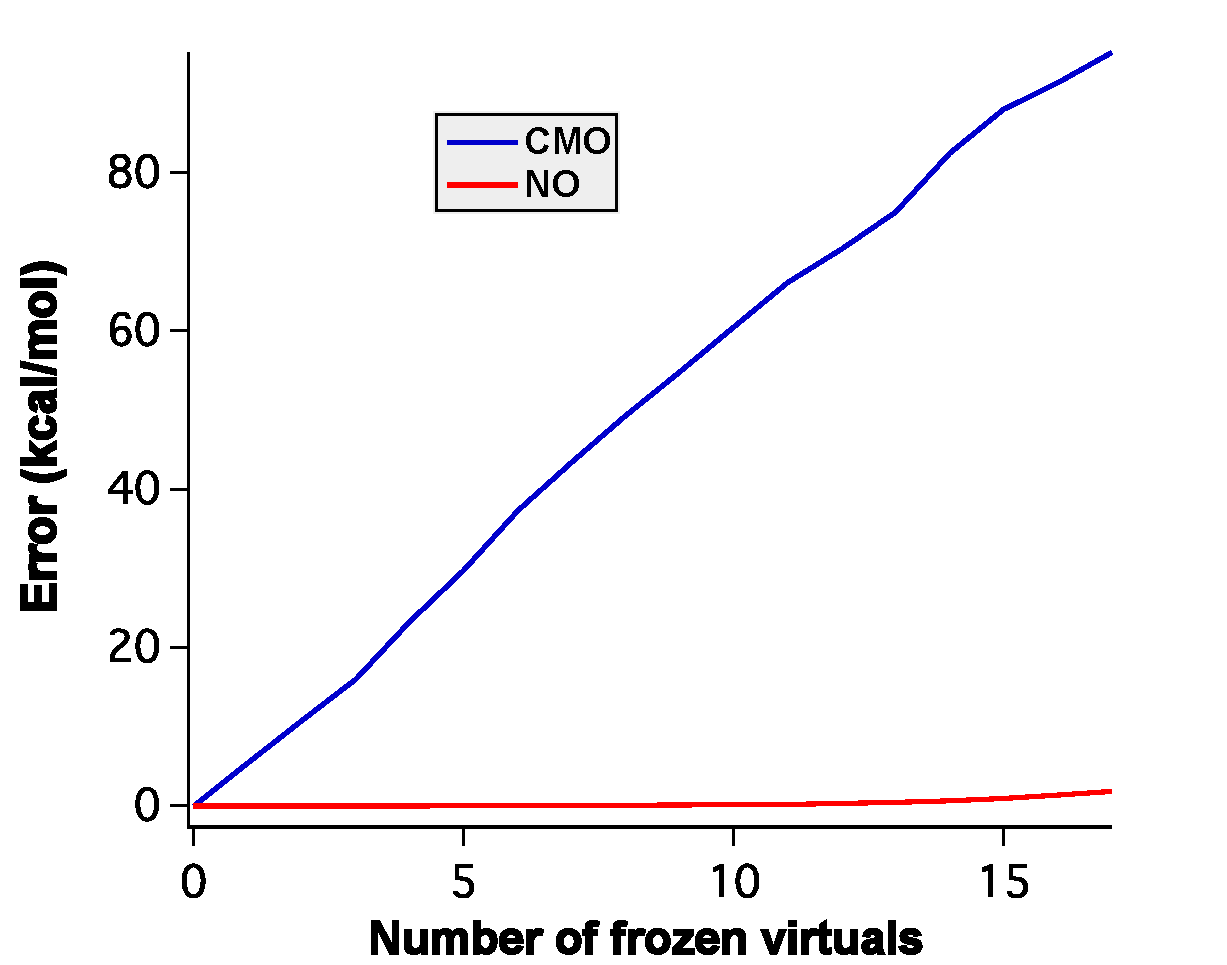
\includegraphics[width=0.7\linewidth]{figures/energy.pdf}
  \caption{Error in the CCSD energy of H$_2$O$_2$ in kcal/mol as a 
           function of the number of frozen virtual orbitals in both CMO and NO bases.} 
  \label{fig:energy}
\end{figure}
%%%%%%%%%%%%%%%%%%%%%%%%%%%%%%%%%%%%%%%%%%%%%%%%%%%%%%%%%%%%%%%
\begin{figure}
  \centering
  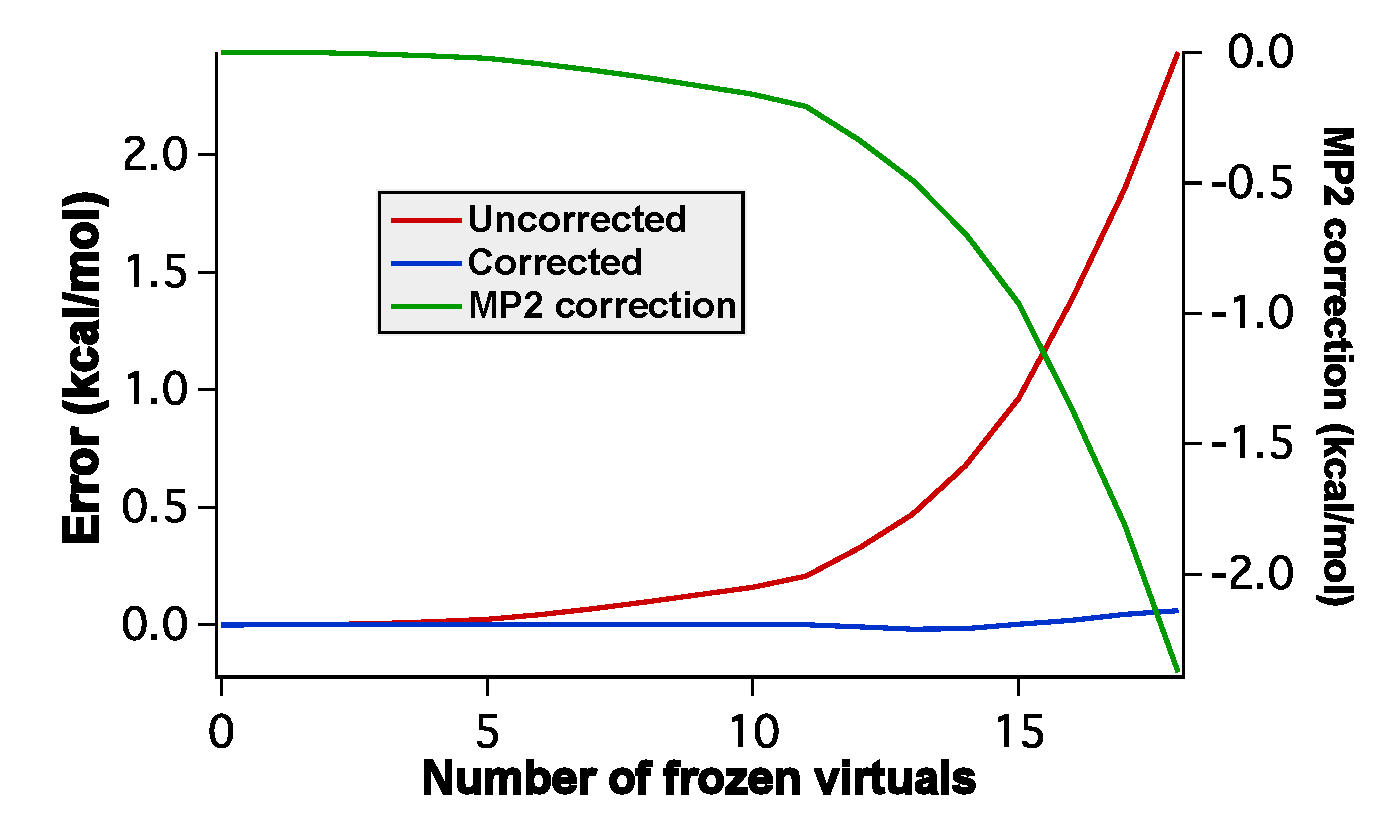
\includegraphics[width=0.7\linewidth]{figures/Mp2c.pdf}
  \caption{Error in CCSD energy of H$_2$O$_2$ in the NO bases, with and without MP2 corrections 
        and MP2 correction as a function of the number of frozen virtual orbitals.}
\label{fig:MP2_corr}
\end{figure}
%%%%%%%%%%%%%%%%%%%%%%%%%%%%%%%%%%%%%%%%%%%%%%%%%%%%%%%%%%%%%%%
\begin{figure}
  \centering
  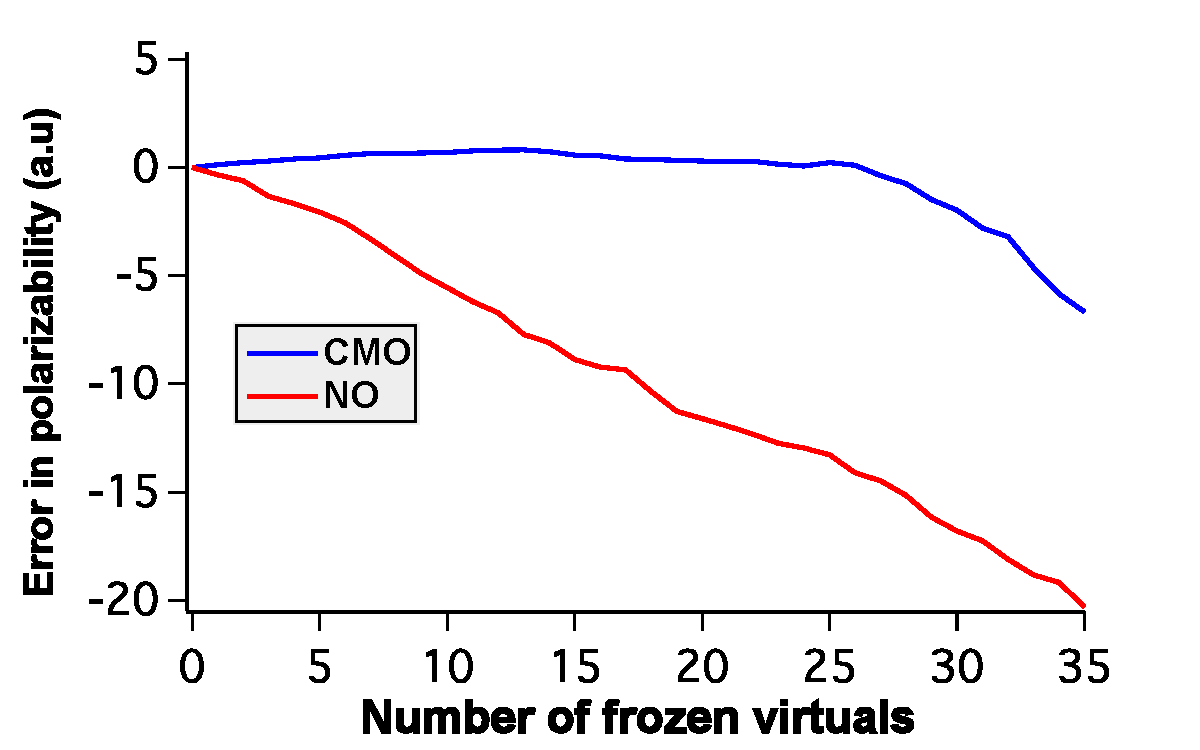
\includegraphics[width=0.6\linewidth]{figures/h2o2_polar.pdf}
  \caption{Errors in the CCSD/aDZ dynamic polarizability (589
nm) of H$_2$O$_2$ in 
       in both CMO and NO bases as a function of number of virtual orbitals removed.}
   \label{fig:polar_h2o2}
\end{figure}
%%%%%%%%%%%%%%%%%%%%%%%%%%%%%%%%%%%%%%%%%%%%%%%%%%%%%%%%%%%%%%%
\begin{figure}
  \centering
  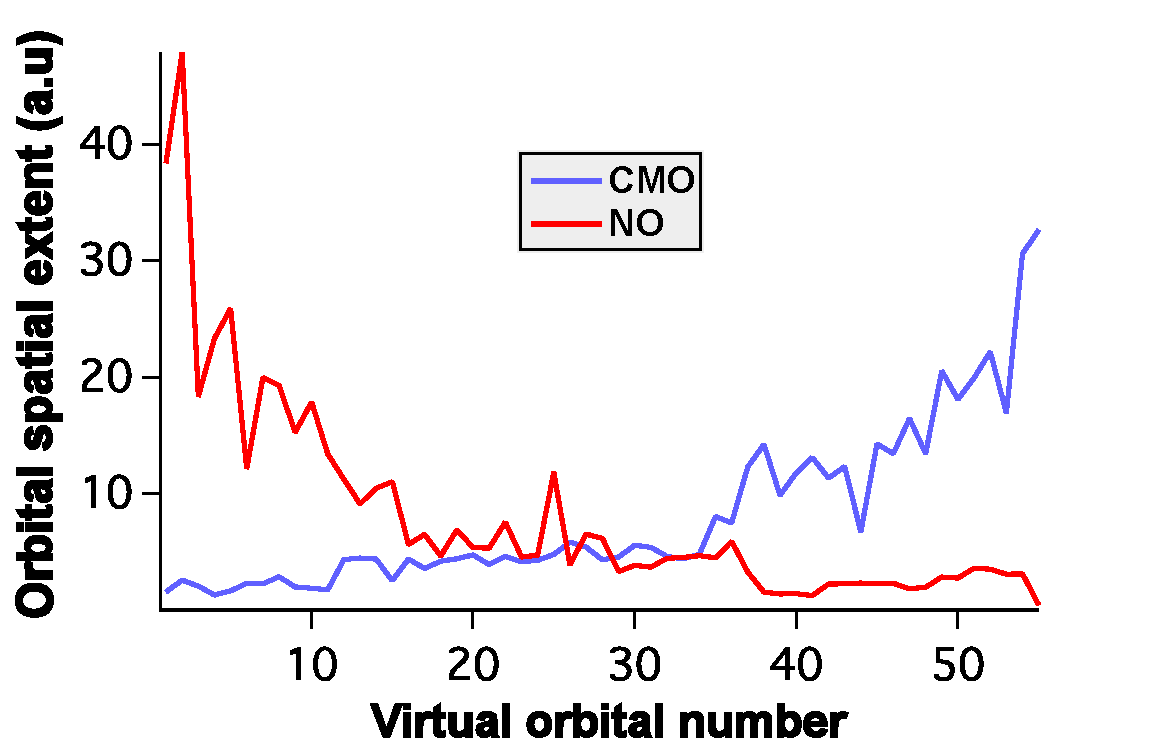
\includegraphics[width=0.6\linewidth]{figures/spatial.pdf}
  \caption{Spatial extent ($\langle r^2\rangle$) of virtual
orbitals of H$_2$O$_2$ in both CMO and NO bases.  Orbitals are ordered
left-to-right by
decreasing energy (CMOs) or increasing occupation number (NOs).}
   \label{fig:spatial}
\end{figure}

%%%%%%%%%%%%%%%%%%%%%%%%%%%%%%%%%%%%%%%%%%%%%%%%%%%%%%%%%%%%%%%
\begin{figure}
  \centering
  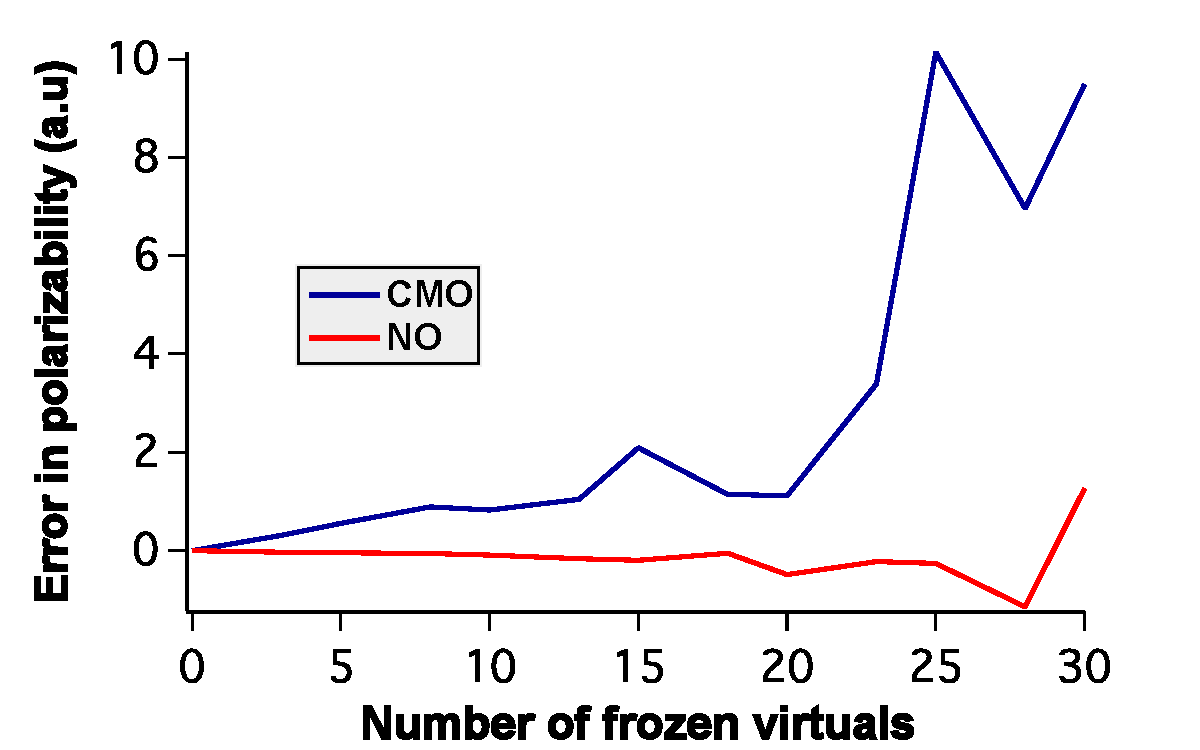
\includegraphics[width=0.6\linewidth]{figures/polar_static.pdf}
  \caption{Errors in the CCSD/aDZ static polarizability 
(including orbital relaxation effects) of H$_2$O$_2$ in
       in both CMO and NO bases as a function of number of virtual orbitals
removed.}
   \label{fig:static}
\end{figure}

%%%%%%%%%%%%%%%%%%%%%%%%%%%%%%%%%%%%%%%%%%%%%%%%%%%%%%%%%%%%%%%
\begin{figure}
  \centering
  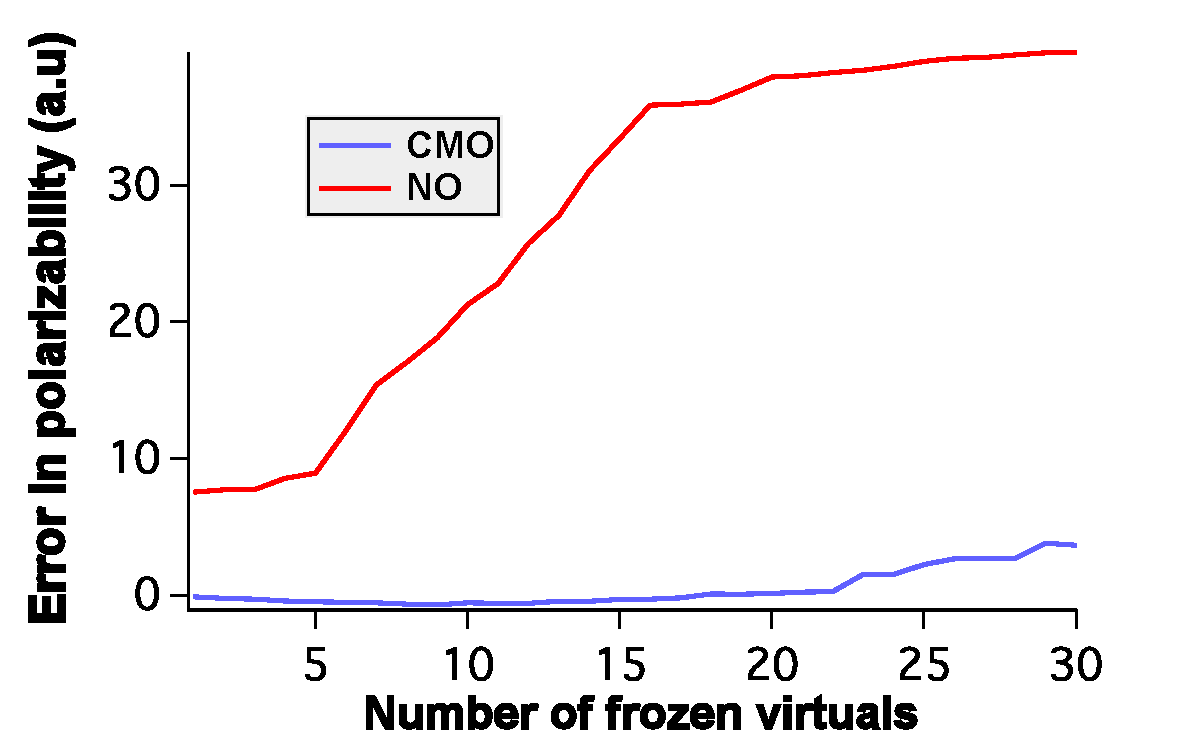
\includegraphics[width=0.6\linewidth]{figures/sort_spatial.pdf}
  \caption{Errors in the CCSD/aDZ dynamic polarizability (589
nm) of H$_2$O$_2$ as a function of the number of virtual CMOs or NOs deleted,
ordered by increasing spatial extent, $\langle r^2 \rangle$.}
   \label{fig:sort_spatial}
\end{figure}
%%%%%%%%%%%%%%%%%%%%%%%%%%%%%%%%%%%%%%%%%%%%%%%%%%%%%%%%%%%%%%%
\begin{figure}
  \centering
  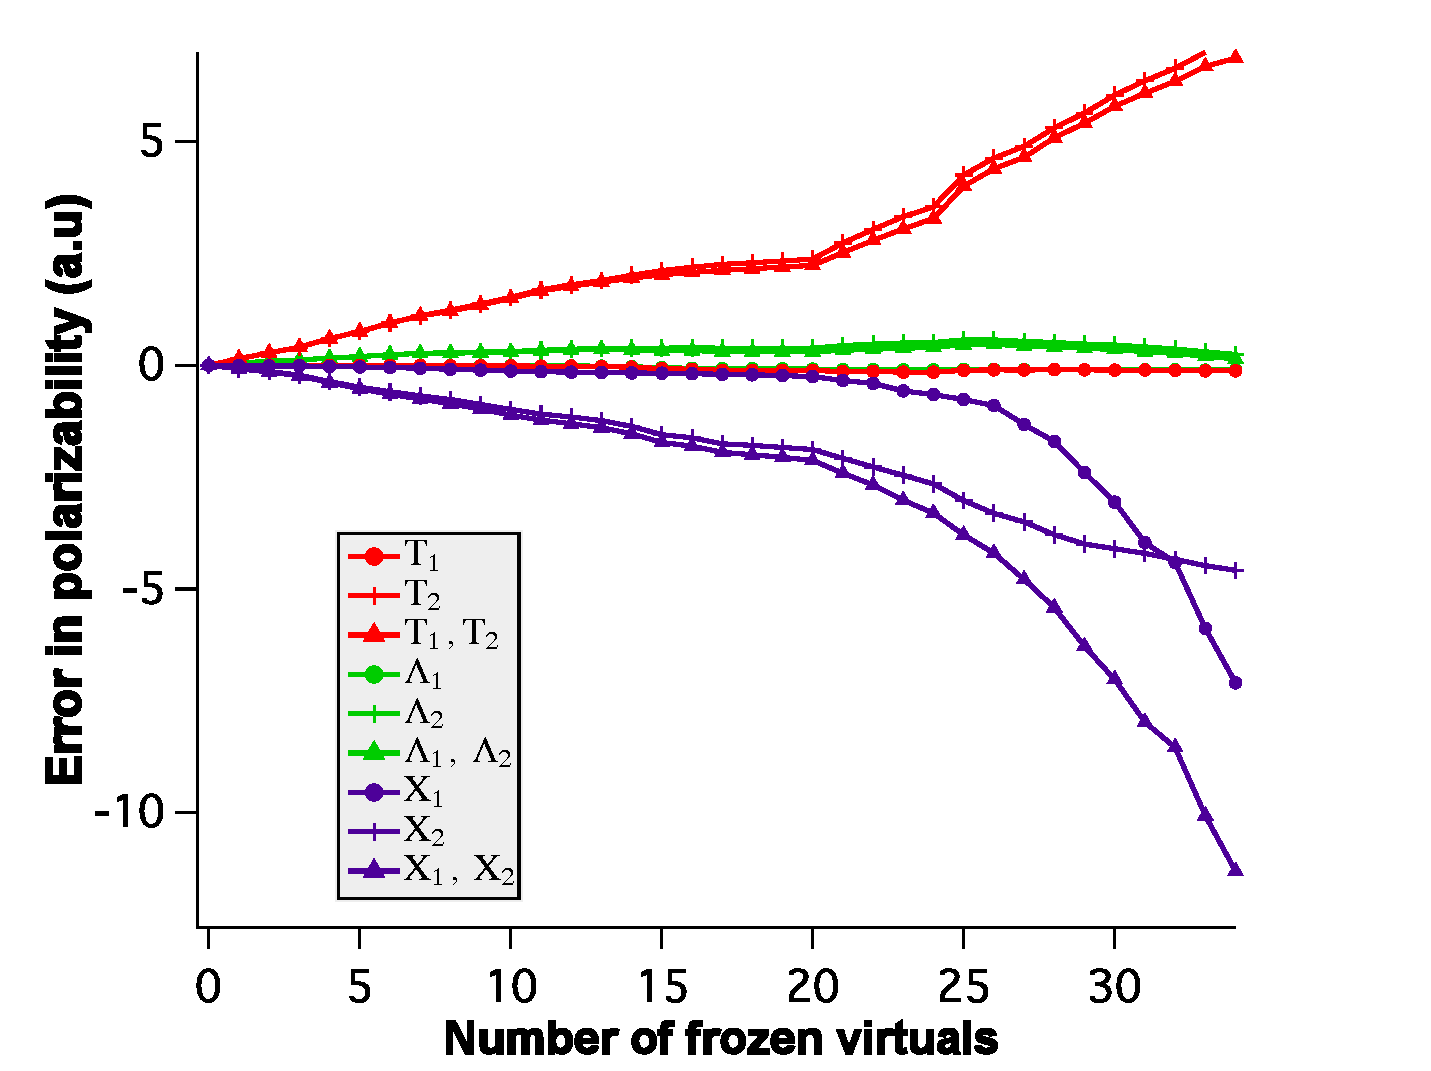
\includegraphics[width=0.6\linewidth]{figures/amp_trunc_cmo.pdf}
  \caption{Errors introduced in CCSD/aDZ polarizabilities of
H$_2$O$_2$ in the virtual CMO bases by the truncation of different classes of wave
function amplitudes.}
   \label{fig:amp_trunc_cmo}
\end{figure}
%%%%%%%%%%%%%%%%%%%%%%%%%%%%%%%%%%%%%%%%%%%%%%%%%%%%%%%%%%%%%%%
\begin{figure}
  \centering
  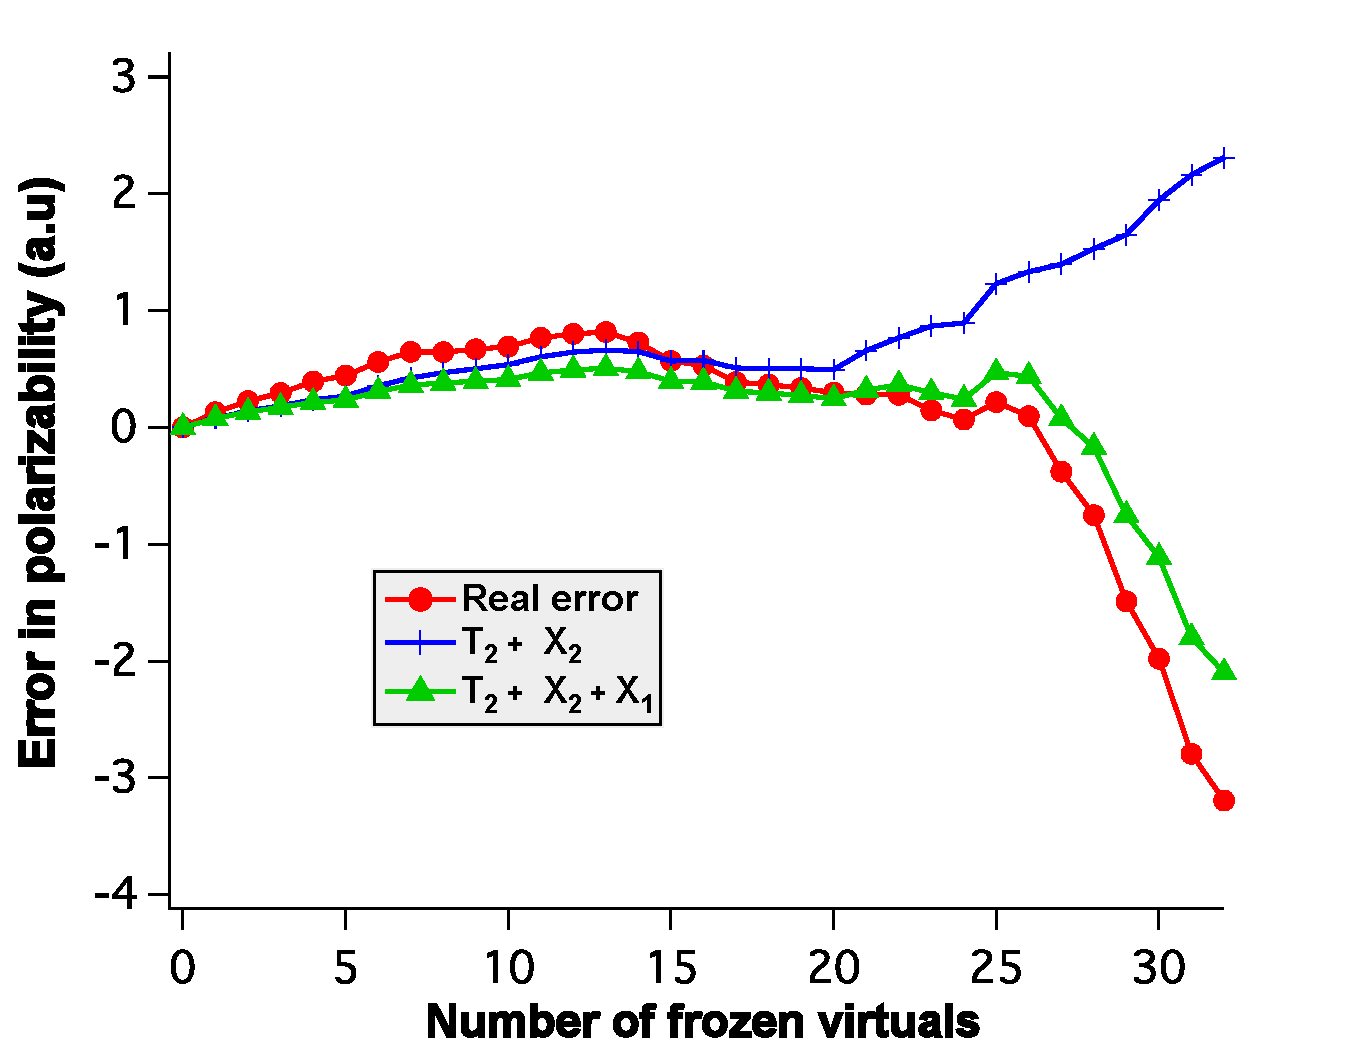
\includegraphics[width=0.6\linewidth]{figures/error_cmpare.pdf}
  \caption{Errors introduced in CCSD/aDZ polarizabilities of
H$_2$O$_2$ in the virtual CMO bases by the truncation of specific classes of wave
function amplitudes as compared to the total errors obtained by freezing of
virtual CMOs.}
   \label{fig:error_compare}
\end{figure}
%%%%%%%%%%%%%%%%%%%%%%%%%%%%%%%%%%%%%%%%%%%%%%%%%%%%%%%%%%%%%%%
\begin{figure}
  \centering
  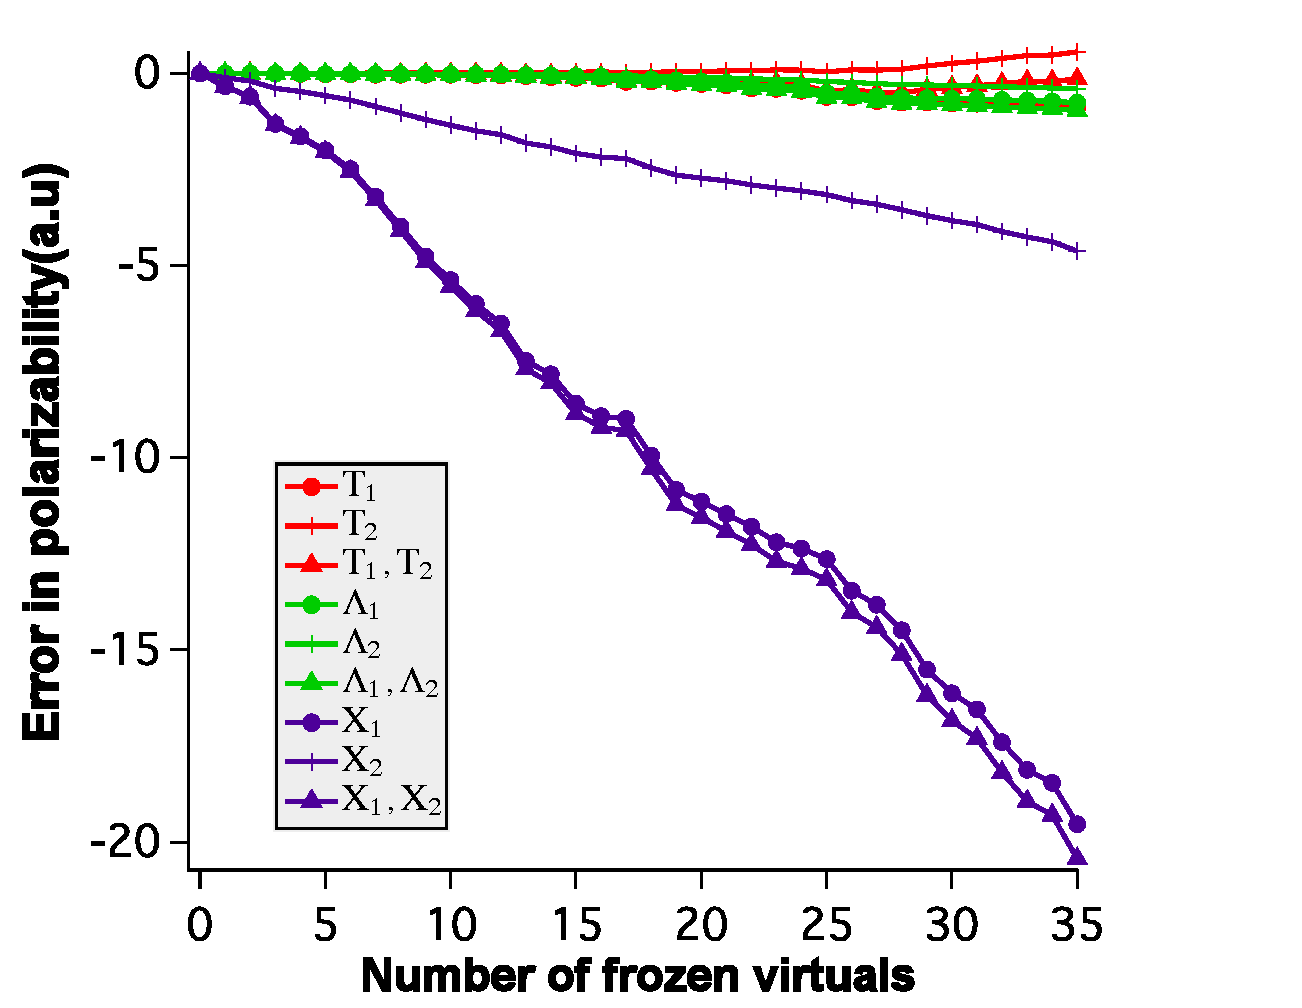
\includegraphics[width=0.6\linewidth]{figures/amp_trunc_no.pdf}
  \caption{Errors introduced in CCSD/aDZ polarizabilities of
H$_2$O$_2$ in the virtual NO bases by the truncation of different classes of wave
function amplitudes.}
   \label{fig:amp_trunc_no}
\end{figure}
%%%%%%%%%%%%%%%%%%%%%%%%%%%%%%%%%%%%%%%%%%%%%%%%%%%%%%%%%%%%%%%
\begin{figure}
  \centering
  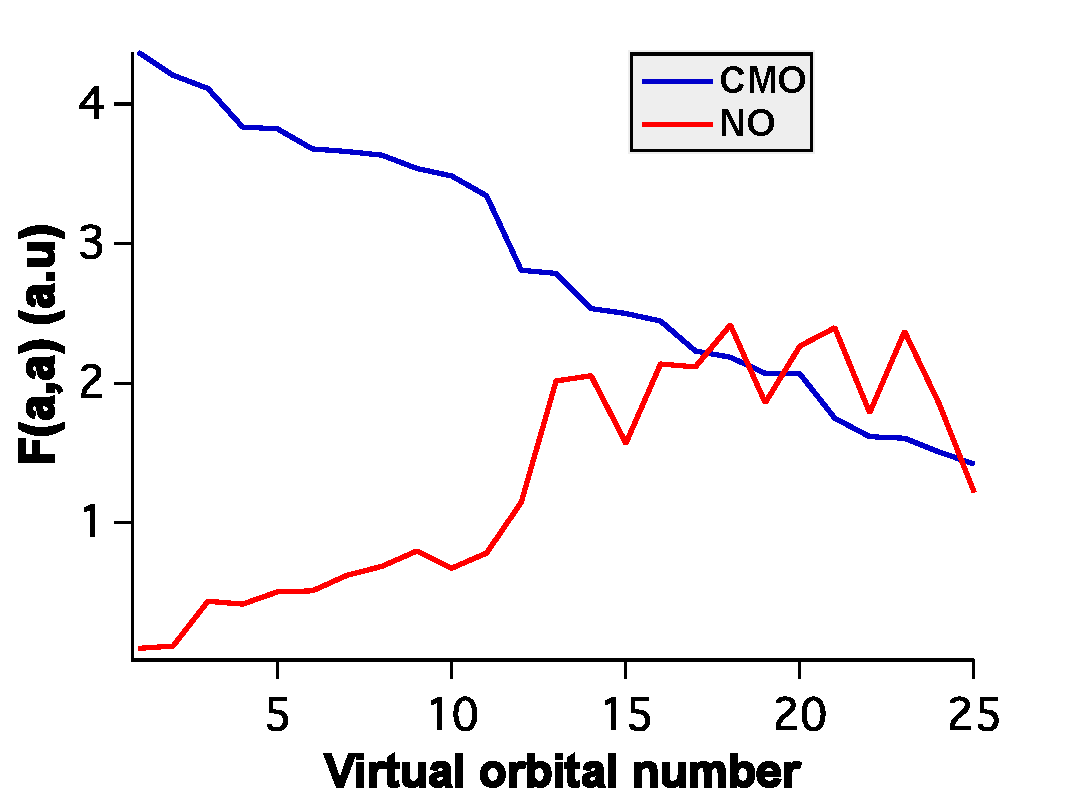
\includegraphics[width=0.6\linewidth]{figures/Faa.pdf}
  \caption{Virtual diagonal elements (a.u.) of the Fock matrix in
the CMO and NO bases.}
   \label{fig:Faa}
\end{figure}
%%%%%%%%%%%%%%%%%%%%%%%%%%%%%%%%%%%%%%%%%%%%%%%%%%%%%%%%%%%%%%%
\begin{figure}
  \centering
  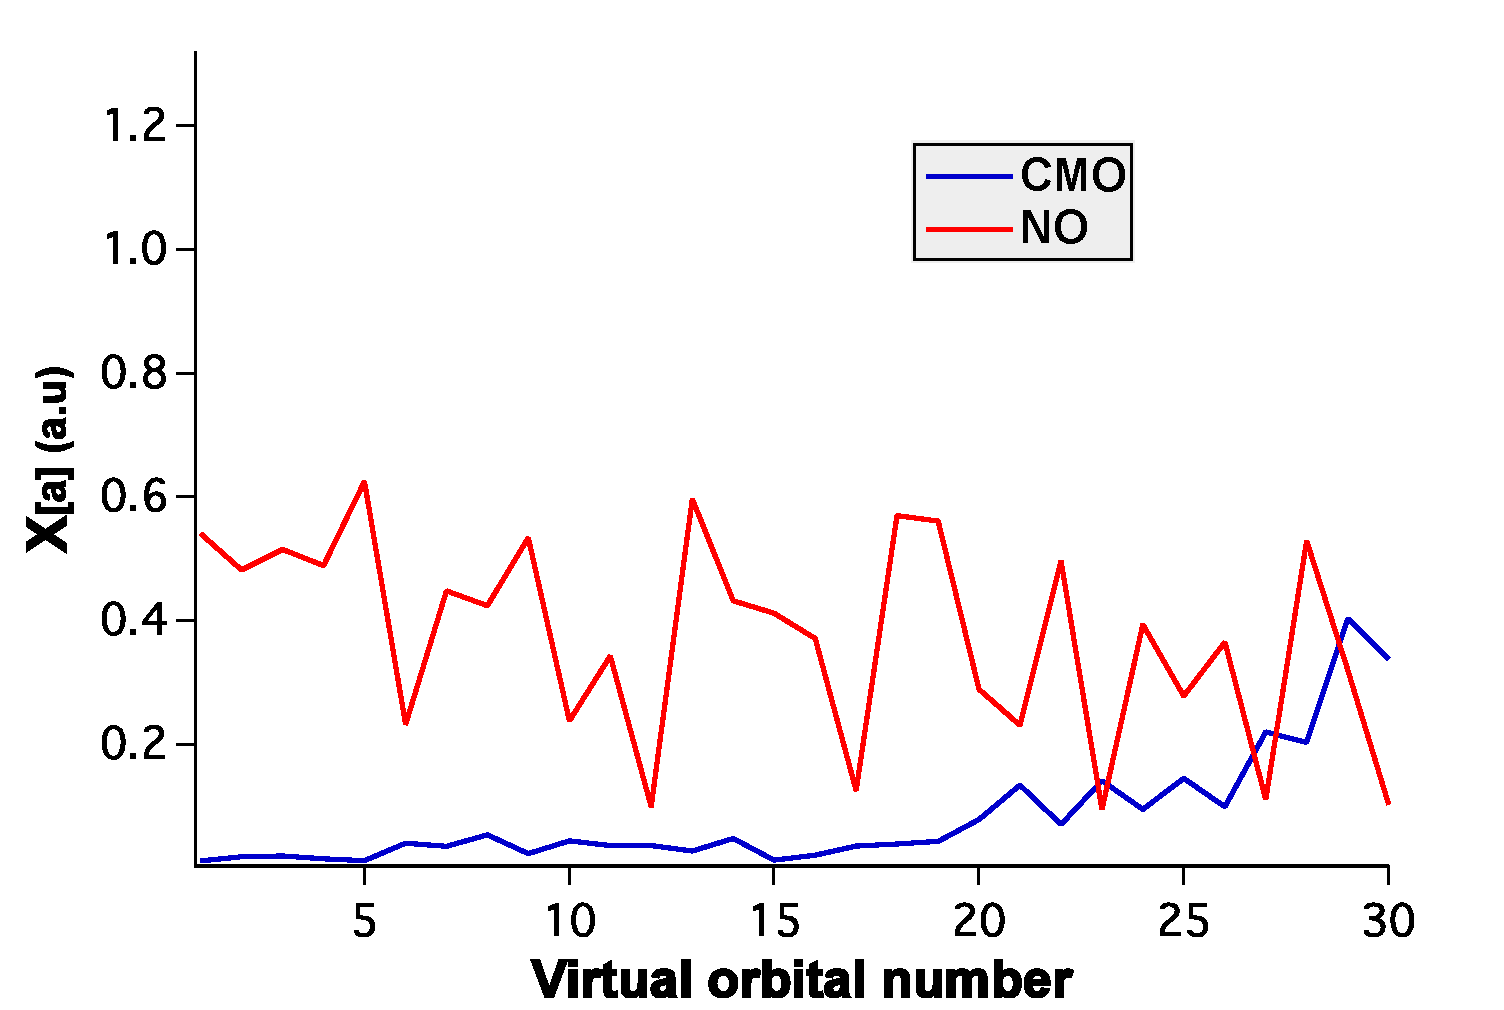
\includegraphics[width=0.6\linewidth]{figures/X1.pdf}
  \caption{Sum of the absolute values of $\hat{X}_1$
amplitudes for a given virtual, $\sum_i \left|X_i^a\right|$, for perturbation $\mu_x$
and frequency 589 nm, plotted for each virtual NO or CMO.}
   \label{fig:X1}
\end{figure}
%%%%%%%%%%%%%%%%%%%%%%%%%%%%%%%%%%%%%%%%%%%%%%%%%%%%%%%%%%%%%%%
\begin{figure}
  \centering
  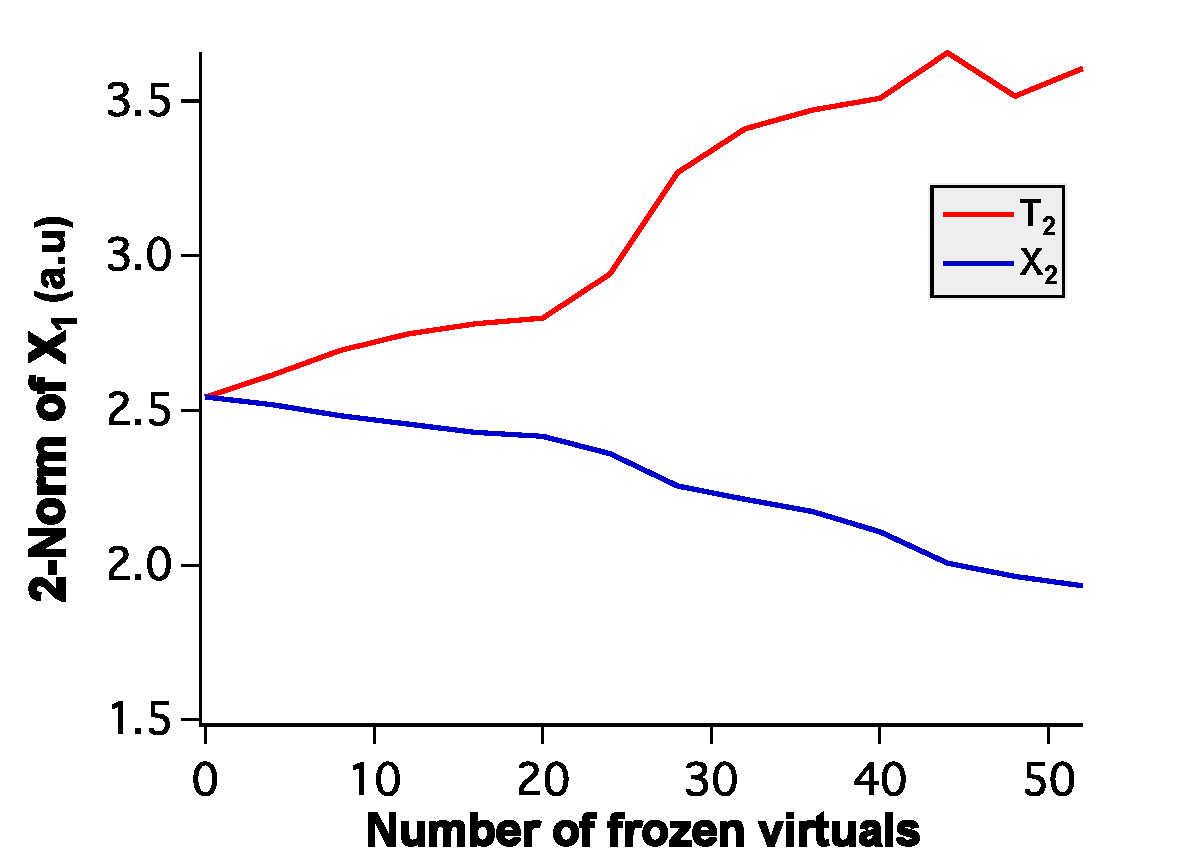
\includegraphics[width=0.6\linewidth]{figures/norm.pdf}
  \caption{The 2-norm of the $\hat{X}_1$ amplitude vector in
the CMO bases as a function of the truncation of classes of unperturbed 
$\hat{T}_2$ and perturbed $\hat{X}_2$ amplitudes.}
   \label{fig:norm}
\end{figure}
%%%%%%%%%%%%%%%%%%%%%%%%%%%%%%%%%%%%%%%%%%%%%%%%%%%%%%%%%%%%%%%
%\begin{figure}
%  \centering
%  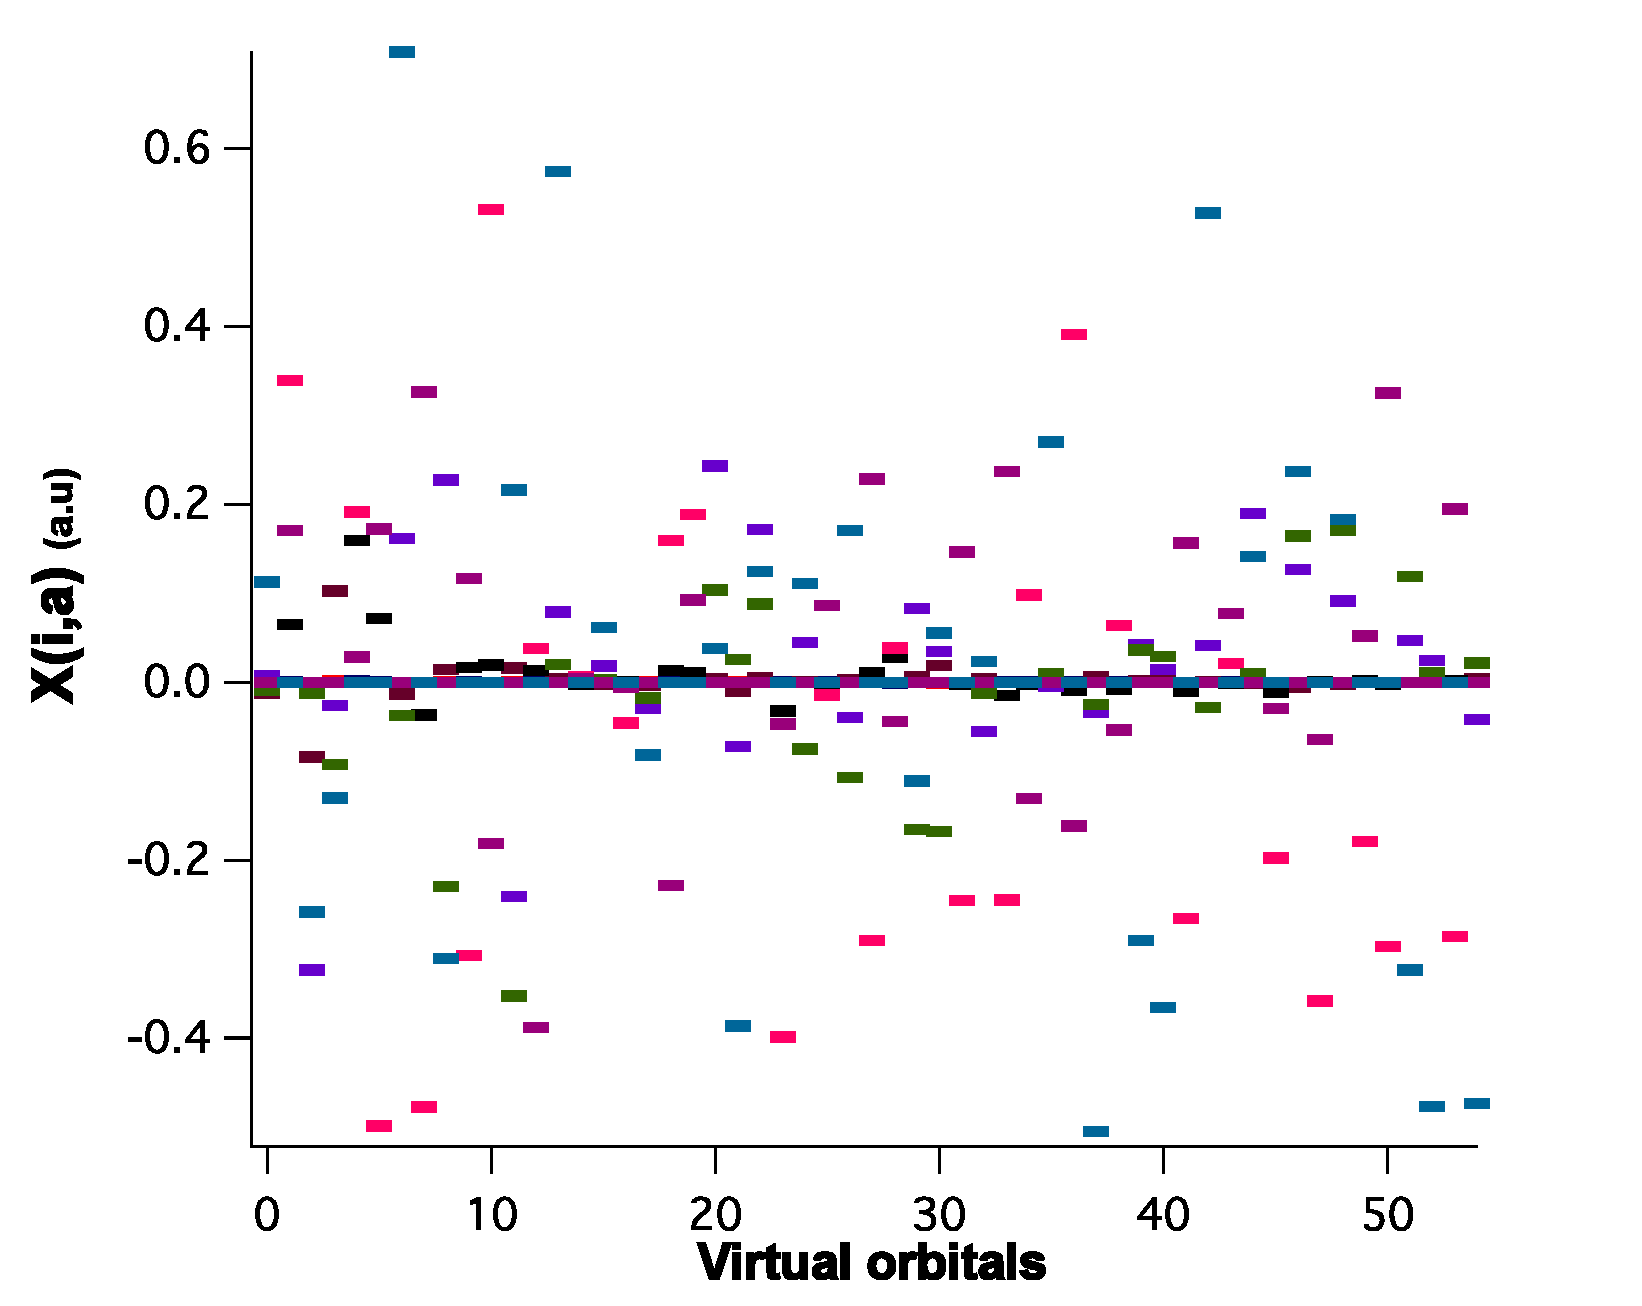
\includegraphics[width=0.6\linewidth]{figures/X1_no.pdf}
%  \caption{\footnotesize{$X_1$ amplitudes $X^{\mu_x}_{ia}$(589 nm) in the NO basis. For each virtual orbital there are nine virtual-occupied pairs.}}
%   \label{fig:X1_no}
%\end{figure}
%%%%%%%%%%%%%%%%%%%%%%%%%%%%%%%%%%%%%%%%%%%%%%%%%%%%%%%%%%%%%%%
\begin{figure}
  \centering
  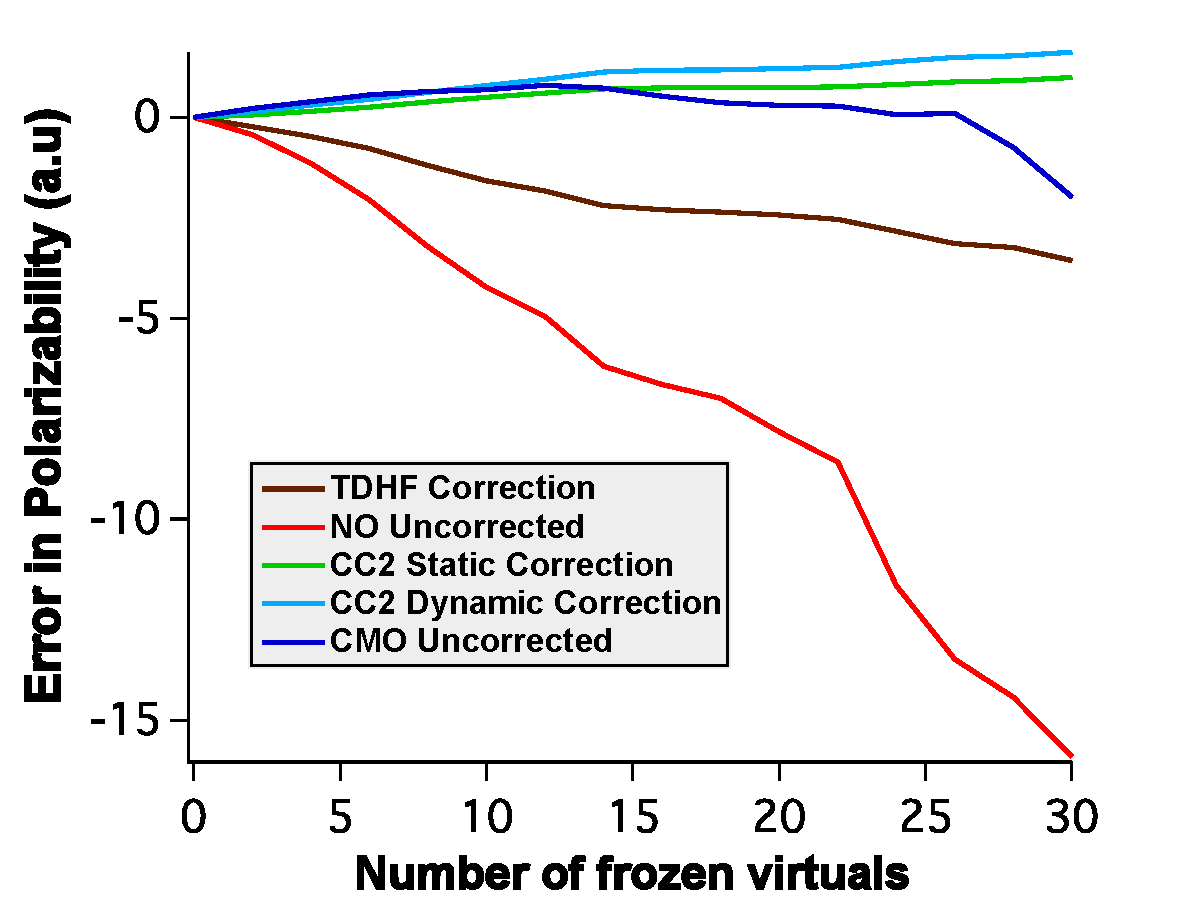
\includegraphics[width=0.6\linewidth]{figures/correctn.pdf}
  \caption{Correction schemes for the external truncated
NO space for the CCSD/aDZ polarizabilities of H$_2$O$_2$.}
   \label{fig:corrections}
\end{figure}
%%%%%%%%%%%%%%%%%%%%%%%%%%%%%%%%%%%%%%%%%%%%%%%%%%%%%%%%%%%%%%%

\begin{figure}
  \centering
  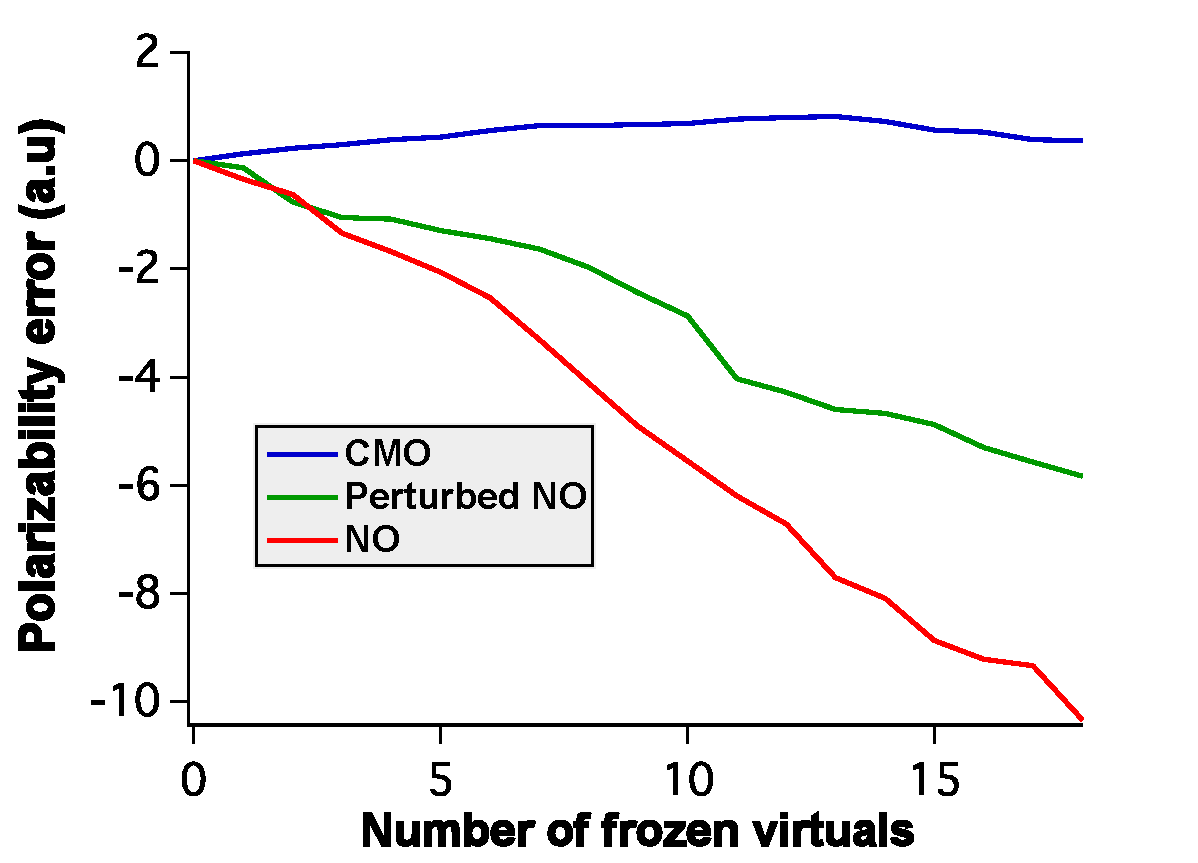
\includegraphics[width=0.6\linewidth]{figures/perturbed.pdf}
  \caption{Errors introduced in CCSD/aDZ polarizabilities of
H$_2$O$_2$ in the virtual CMO and NO bases, as well as the perturbed
virtual NO basis as a function of number of virtual orbitals removed.}
   \label{fig:perturb}
\end{figure}
%%%%%%%%%%%%%%%%%%%%%%%%%%%%%%%%%%%%%%%%%%%%%%%%%%%%%%%%%%%%%%%
\begin{figure}
  \centering
  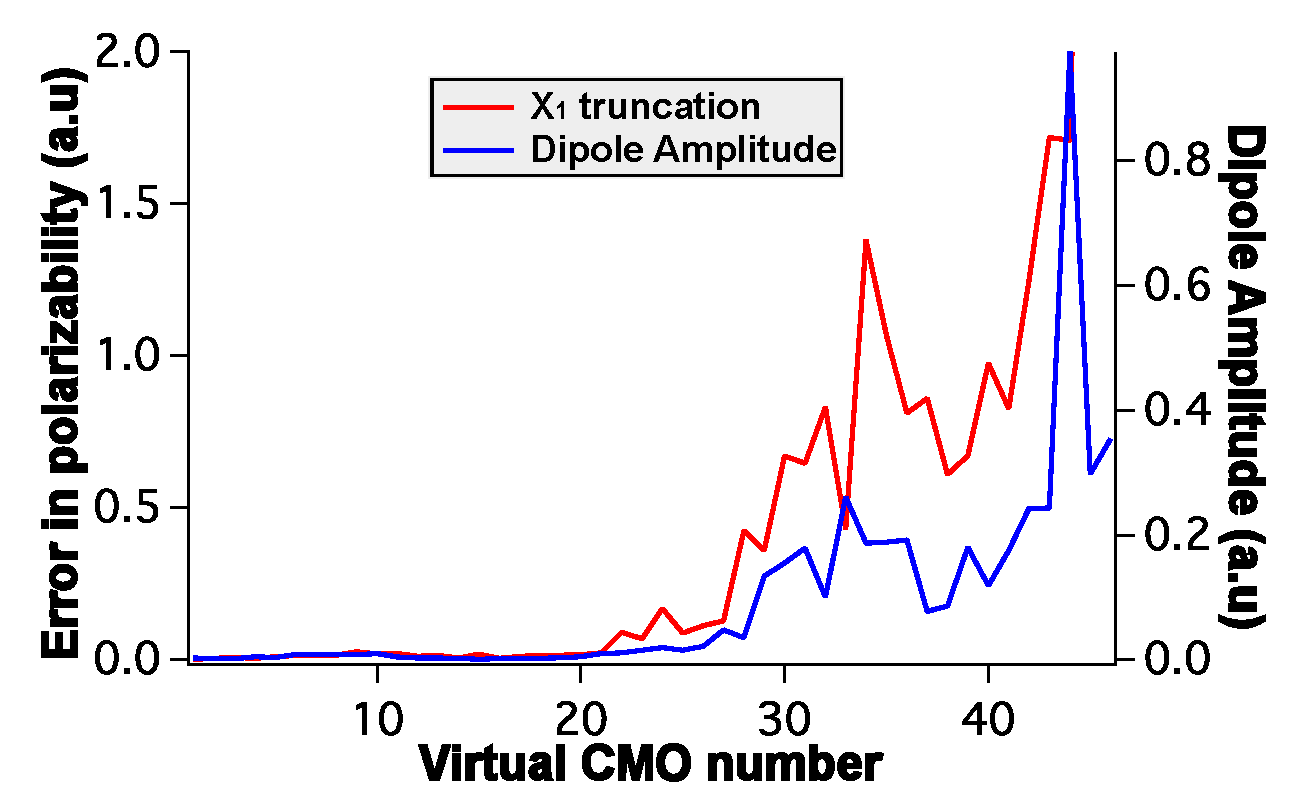
\includegraphics[width=0.6\linewidth]{figures/diplength.pdf}
  \caption{Absolute errors introduced in CCSD/aDZ
  polarizabilities of H$_2$O$_2$ due to truncation of $\hat{X}_1$ amplitudes and
  dipole amplitudes plotted as a function of different virtual CMOs.}
   \label{fig:dipole_length}
\end{figure}
%%%%%%%%%%%%%%%%%%%%%%%%%%%%%%%%%%%%%%%%%%%%%%%%%%%%%%%%%%%%%%%


\newpage
\begin{center}
{\bf TOC Graphic}
\includegraphics[width=1.0\linewidth]{figures/toc.png}
\end{center}

%
%\end{document}

\chapter{Conclusions}
\markright{Ashutosh Kumar \hfill Chapter 6. Conclusions\hfill}
Reduced-scaling techniques have extended the application of accurate coupled cluster (CC)
methods to molecules with hundreds of heavy atoms\cite{Neese09,NeeseCCSD09}. However, efforts towards extension 
of these schemes to simulate linear response properties have been fairly 
limited\cite{Gauss00,Korona04,Russ04,McAlexander12,Friedrich15,Russ08}. McAlexander and Crawford\cite{McAlexander15:LRCC} recently compared the performances of
reduced-scaling methods based on projected atomic orbitals (PAOs)\cite{Saebo86,Pulay83,PulaySaebo93}, orbital specific virtuals (OSVs)\cite{Yang12} and pair natural orbitals (PNOs)\cite{Edmiston66,Meyer73,Ahlrichs75,Neese09} for calculating optical rotations using the
coupled cluster linear response theory\cite{Koch90}, where they found the PNOs to be the most compact 
representation of the virtual space. However, very tight cutoffs needed to be employed in order to 
match the canonical results. \\
In our search for an optimal virtual space for response calculations,
we investigated the performance of the frozen virtual natural orbital (FVNO) scheme,
(chapter 3) which had been applied quite successfully to bring down the 
computational costs of CC calculations involving energies, geometry optimizations, 
ionization enthalpies, etc.\cite{Sosa89,Taube05,Taube08,Landau10,DePrince13:FNOs,DePrince13}, 
for calculating dynamic polarizabilities of 
small chiral compounds\cite{Kumar17}. It was found that the virtual natural orbitals (VNOs)
obtained from the ground state MP2 density (GSMP2D) are not suitable for calculating 
polarizabilities (and hence optical rotations) in the absence of orbital relaxation 
effects as the shift in their values with respect to the full canonical result grew 
almost linearly with the number of truncated VNOs. However, introduction of orbital
relaxation can introduce spurious or unphysical poles in the linear response function
because of which they are not included in the CC linear response calculations.
On a closer inspection, we found that all the diffuse 
VNOs had very low occupation numbers (ONs) and thus were removed first
in this scheme resulting in large errors. It should be noted that these 
diffuse orbitals are absolutely essential for calculating chiroptical properties 
as many chiral molecules posess low lying Rydeberg type excited states.
We also employed a CC2\cite{Christiansen95:CC2} based correction for the external truncated 
space which was able to reduce the errors drastically, but such an approach 
could not lead to any computational savings. Finally, we constructed a first 
order perturbed density by taking the derivative of the GSMP2D with 
respect to an external electric field, with the hope that the occupation 
numbers (ONs) generated using this density would be a better metric for 
estimating the importance of a VNO for describing the response of the 
wavefunction. However, this approach offered only marginal improvement 
in the errors. On the other hand, truncating canonical molecular orbitals (CMOs) 
with high orbital energies resulted in very small errors (less than 2\% after 
removing 50\% of the virtual space) due to intrinsic cancellation of errors.\\
On the basis of the above findings, we tried out a modified FVNO scheme, FVNO(M)
in Chapter 4, where the virtual CMOs (VCMOs) were sorted according to their diffusivity which 
wa measured by the values of their orbital spatial extents (OSEs) and GSMP2D was 
built only in the space of non-diffuse (under a given OSE cutoff) orbitals. 
In other words, the diffuse part of the virtual space remains unaffected 
by the FVNO procedure. Pilot studies on H$_2$O$_2$ molecule showed that the
FVNO(M) method yielded minimal errors compared to the original scheme 
for polarizabilities, optical rotations, rotational strengths, 
excitation energies, etc. However, more systematic studies are needed to 
make it a truly black-box method. We also looked at the perturbed density 
model in more details by first constructing the (full) CCSD first order 
perturbed density. It was found that the diagonal elements of this density 
matrix are always zeros irrespective of the perturbation. Clearly, the VNOs
obtained by the diagonalization of such densities don't carry any useful information.
Ideally, the structure of the perturbed density should be able to mimic these (linear response) properties 
which are second order in the perturbation. Hence, we proposed a new approach called
FVNO++, where a second-order perturbed density is constructed and then diagonalized
to define the virtual space. Pilot studies on H$_2$O$_2$ molecule and chiral linear chain
hydrogen helices ((P)-$(H_2)_n$) using the FVNO++ approach have shown quite promising results 
for both polarizabilities and optical rotations. The major advantage of this approach 
over FVNO(M) is that ONs are a much more robust truncation criterion compared to the OSEs.\\
%However, calculations with other choices of perturbed densities also need to be
%done, especially for bigger molecules to make the FVNO++ truncation scheme truly robust.
%We are currently in the process of a RI-CC2 linear response code\cite{} which we intend
%to use in conjunction with the FVNO++ formalism to tackle larger molecular systems.
%Furthermore, we propose to extend this approach to the reduced-scaling techniques based
%on pair natural orbitals\cite{}.
We extended the above analyses to the PNO domain in Chapter 5 as the  
the PNOs can be seen as an extension of the concept of 
natural orbitals. Consequently, the PNO(M) method was designed where
all the diffuse VCMOs were retained and every pair of occupied orbitals
inherited this global virtual space. Just as before, PNO(M) significantly
accelerates the convergence of these properties towards the full
canonical result. However, this means that every occupied pair becomes a 
strong pair and hence can't be neglected, which has an adverse affect
on the reduced scaling capabilities of the PNO scheme. Along the 
lines of FVNO++, PNO++ approach was formulated where the structure of 
the pair specific densities resemble with the contributions of a given
pair to the response functions. Preliminary results on chiral linear chain 
hydrogen helices indicate a performance similar to the PNO(M) approach
for both polarizabilities and optical rotations. However, calculations on 
two and three dimensional structures involving different forms of second-order 
perturbed densities need to be carried out in order to make PNO++ a truly robust method. \\
Encouraged by the performances of these methods, we plan to use them in 
conjunction with density-fitted CC linear response codes\cite{Friese12} to target larger
systems like solvated molecular clusters. We assume that a larger solvent shell 
around the solute molecule would require comparitively smaller number of 
snapshots for the optical rotations to converge to the experimental value. Thus, we can significantly
lower down the computational costs involved in CC calculations of optical rotations
of solvated molecules.

\markright{Ashutosh Kumar \hfill Chapter 6. Conclusions\hfill}
%%%%%%%%%%%%%%%%%
%
% Include an EPS figure with this command:
%   \epsffile{filename.eps}
%

%%%%%%%%%%%%%%%%
%
% Do tables like this:

% \begin{table}
% \caption{The Graduate School wants captions above the tables.}
%\begin{center}
% \begin{tabular}{ccc}
% x & 1 & 2 \\ \hline
% 1 & 1 & 2 \\
% 2 & 2 & 4 \\ \hline
% \end{tabular}
%\end{center}
% \end{table}

%%%%%%%%%%%%%%%%%%%%%%%%%%%%%%%%

% If you are using BibTeX, uncomment the following:
%\thebibliography
%\begin{thebibliography}{99}
%\bibitem{Shavitt09}I. Shavitt and R. J. Bartlett. Many-Body Methods in Chemistry and
%Physics: MBPT and Coupled-Cluster Theory; Cambridge University
%Press: Cambridge, 2009. 
%\end{thebibliography}
%\bibliographystyle{unsrt}
%\chapter*{Bibliography}

\chapter*{Appendix A\\Publication List}
\begin{enumerate}
\item A. Kumar and T. D. Crawford, J. Phys. Chem. A, 2017, 121(3), pp 708-716.
\item A. Kumar and T. D. Crawford, J. Phys. Chem. A, 2017, 121(3), pp 708-716.
\item A. Kumar and T. D. Crawford, J. Phys. Chem. A, 2017, 121(3), pp 708-716.
\item A. Kumar and T. D. Crawford, J. Phys. Chem. A, 2017, 121(3), pp 708-716.
\item A. Kumar and T. D. Crawford, J. Phys. Chem. A, 2017, 121(3), pp 708-716.
\end{enumerate}

%\bibliographystyle{plain}
%\bibliography{refs}
%\markright{Ashutosh Kumar \hfill Bibliography\hfill}
%\chapter*{Appendix A\\Publication List}
%\begin{enumerate}
\item A. Kumar and T. D. Crawford, J. Phys. Chem. A, 2017, 121(3), pp 708-716.
\item A. Kumar and T. D. Crawford, J. Phys. Chem. A, 2017, 121(3), pp 708-716.
\item A. Kumar and T. D. Crawford, J. Phys. Chem. A, 2017, 121(3), pp 708-716.
\item A. Kumar and T. D. Crawford, J. Phys. Chem. A, 2017, 121(3), pp 708-716.
\item A. Kumar and T. D. Crawford, J. Phys. Chem. A, 2017, 121(3), pp 708-716.
\end{enumerate}

%\bibliography{papes}
%
% Otherwise, uncomment the following:
%\chapter*{Appendix A\\Publication List}
%\begin{enumerate}
\item A. Kumar and T. D. Crawford, J. Phys. Chem. A, 2017, 121(3), pp 708-716.
\item A. Kumar and T. D. Crawford, J. Phys. Chem. A, 2017, 121(3), pp 708-716.
\item A. Kumar and T. D. Crawford, J. Phys. Chem. A, 2017, 121(3), pp 708-716.
\item A. Kumar and T. D. Crawford, J. Phys. Chem. A, 2017, 121(3), pp 708-716.
\item A. Kumar and T. D. Crawford, J. Phys. Chem. A, 2017, 121(3), pp 708-716.
\end{enumerate}

\chapter*{Appendix B \\ Supporting Information for ``Frozen Virtual Natural Orbitals for
Coupled Cluster Linear-Response Theory"}
%\pagebreak
%\appendix{Appendix}
\markright{Ashutosh Kumar \hfill Appendix B. FVNO SI\hfill}
\documentclass[journal=jpccck,manuscript=article]{achemso}

\usepackage{graphicx}
\usepackage{xcolor}
\usepackage[utf8]{inputenc} % set input encoding (not needed with XeLaTeX)
\usepackage{verbatim}
\usepackage{amsfonts}
\usepackage{graphicx}
\usepackage{multirow}
\usepackage{array}
\usepackage{varwidth}
\usepackage{bm}

\renewcommand\thetable{S\arabic{table}}
\renewcommand\thefigure{S\arabic{figure}}

\title{Supporting Information for ``Frozen Virtual Natural Orbitals for
Coupled Cluster Linear-Response Theory"}
\author{Ashutosh Kumar}
\affiliation{Department of Chemistry, Virginia Tech, Blacksburg, Virginia 24061, U.S.A.}
\author{T.\ Daniel Crawford}
\email{crawdad@vt.edu}
\affiliation{Department of Chemistry, Virginia Tech, Blacksburg, Virginia 24061, U.S.A.}

\date{\today}

\begin{document}

\maketitle

\clearpage

\begin{figure}
  \centering
  \includegraphics[width=1.1\linewidth]{SI/polar_adz.pdf}
  \caption{Errors in the CCSD/aDZ dynamic polarizability (589
nm) in both CMO and NO bases as a function of number of virtual orbitals
removed for four additional test cases: (\textit{P})-dimethylallene (DMA),
   (\textit{P})-dimethylallene and one water molecule (DMA1w), (\textit{S})-Methyloxirane
(MOX), and (\textit{S})-Methyloxirane and two water molecules with one of the water
molecules removed leaving only its basis functions.}
   \label{fig:polar_adz}
\end{figure}

\begin{figure}
  \centering
  \includegraphics[width=0.6\linewidth]{SI/h2o2_aTZ_polar.pdf}
  \caption{{\footnotesize Errors in the CCSD/aTZ dynamic polarizability (589 nm) of
H$_2$O$_2$ in in both CMO and NO bases as a function of number of virtual orbitals removed.}
   \label{fig:h2o2_aTZ_polar}}
\end{figure}
\begin{figure}
  \centering
  \includegraphics[width=0.6\linewidth]{SI/h2o2_aQZ_polar.pdf}
  \caption{{\footnotesize Errors in the CCSD/aQZ dynamic polarizability (589 nm) of
H$_2$O$_2$ in in both CMO and NO bases as a function of number of virtual orbitals removed.}}
   \label{fig:h2o2_aQZ_polar}
\end{figure}


\newpage

%\begin{table}[ht]
\begin{table}
\caption{B3LYP/aug-cc-pVDZ optimized geometry (\AA) of hydrogen peroxide.}
\begin{center}
\begin{tabular}{cccc}
\hline
Atomic  symbol & X & Y & Z \\
\hline
\hline
 O &    -0.028962160801 &   -0.694396279686 &   -0.049338350190\\
 O &     0.028962160801 &    0.694396279686 &   -0.049338350190\\
 H &     0.350498145881 &   -0.910645626300 &    0.783035421467\\
 H &    -0.350498145881 &    0.910645626300 &    0.783035421467\\
\hline
\end{tabular}
\end{center}
%\caption{B3LYP/aug-cc-pVDZ optimized geometry (\AA) of hydrogen peroxide.}
\label{table:S2}
\end{table}

% \begin{table}
% \caption{The Graduate School wants captions above the tables.}
%\begin{center}
% \begin{tabular}{ccc}
% x & 1 & 2 \\ \hline
% 1 & 1 & 2 \\
% 2 & 2 & 4 \\ \hline
% \end{tabular}
%\end{center}
% \end{table}

\begin{table}[ht]
\begin{tabular}{cccc}
\hline
Atomic  symbol & X & Y & Z \\
\hline
\hline
C  &  0.00000000   & 0.00000000    &  0.00000000\\  
C  & -0.87382800   & 0.87178900    &  0.87038800\\
C  & -0.87382800   & 2.18536200    &  0.87080500\\
C  & -0.87382800   & 3.49893500    &  0.87038800\\
H  & -0.19165900   & 4.01714100    &  1.55371200\\
C  & -1.74765600   & 4.37072400    &  0.00000000\\
H  & -2.39264800   & 3.76601200    & -0.64911100\\
H  & -2.38616500   & 5.02111900    &  0.61760600\\
H  & -1.13340200   & 5.02895100    & -0.63367100\\
H  & -1.55599700   & 0.35358300    &  1.55371200\\
H  &  0.64499200   & 0.60471200    & -0.64911100\\
H  &  0.63850900   &-0.65039500    &  0.61760600\\
H  & -0.61425400   &-0.65822700    & -0.63367100\\
\hline
\hline
\end{tabular}
\caption{B3LYP/aug-cc-pVDZ optimized geometry (\AA) of (\textit{P})-dimethylallene.}
\label{table:S1}
\end{table}

%
%\begin{table}[ht]
%\begin{tabular}{cccc}
%\hline
%Atomic  symbol & X & Y & Z \\
%\hline
%\hline
% O &    -0.028962160801 &   -0.694396279686 &   -0.049338350190\\ 
% O &     0.028962160801 &    0.694396279686 &   -0.049338350190\\
% H &     0.350498145881 &   -0.910645626300 &    0.783035421467\\
% H &    -0.350498145881 &    0.910645626300 &    0.783035421467\\
%\hline
%\end{tabular}
%\caption{Table S2: $H_2O_2$ geometry.}
%\label{table:S2}
%\end{table}
%
%\begin{table}[ht]
%\begin{tabular}{cccc}
%\hline
%Atomic  symbol & X & Y & Z \\
%\hline
%\hline
%  C &    0.00000000 &   0.00000000 &   0.00000000\\
%  C &   -1.46444400 &  -0.36643000 &   0.02694600\\
%  C &   -2.44105800 &   0.44524100 &   0.36174100\\
%  C &   -3.41923100 &   1.26314500 &   0.68806000\\
%  H &   -3.71780300 &   1.32103000 &   1.74107500\\
%  C &   -4.16801100 &   2.15536700 &  -0.27447800\\
%  H &   -3.80129000 &   2.02991300 &  -1.30007100\\
%  H &   -5.24434000 &   1.92768500 &  -0.25838400\\
%  H &   -4.05435400 &   3.21167600 &   0.01259000\\
%  H &   -1.72145400 &  -1.39204600 &  -0.25890200\\
%  H &    0.15629600 &   1.04448300 &   0.29557800\\
%  H &    0.57342800 &  -0.64609200 &   0.68212100\\
%  H &    0.41596400 &  -0.14458000 &  -1.00872300\\
%  O &   -5.05428200 &  -1.67323100 &  -0.06746500\\
%  H &   -4.46520000 &  -0.94134100 &   0.17201000\\
%  H &   -5.19373900 &  -2.15473700 &   0.75630300\\
%\hline
%\hline
%\end{tabular}
%\caption{Table S3: DMA  + 1 water geometry.}
%\label{table:S3}
%\end{table}
%
%\begin{table}[ht]
%\begin{tabular}{cccc}
%\hline
%Atomic  symbol & X & Y & Z \\
%\hline
%\hline
%   C  &             14.60000000 &   14.52999999 &   15.13000000\\ 
%   O  &             14.60000000 &   14.52999999 &   16.53000000\\
%   C  &             15.85999999 &   14.52999999 &   15.84999999\\
%   C  &             14.51999999 &   15.70999999 &   14.30000000\\
%   H  &             13.57999999 &   15.70999999 &   13.75000000\\
%   H  &             14.58000000 &   16.60000000 &   14.91999999\\
%   H  &             15.35000000 &   15.70999999 &   13.58999999\\
%   H  &             14.08999999 &   13.64000000 &   14.76999999\\
%   H  &             16.43000000 &   13.64000000 &   15.59000000\\
%   H  &             16.43000000 &   15.41999999 &   15.59000000\\
%\hline
%\hline
%\end{tabular}
%\caption{Table S4: MOX geometry.}
%\label{table:S4}
%\end{table}
%
%\begin{table}[ht]
%\begin{tabular}{cccc}
%\hline
%Atomic  symbol & X & Y & Z \\
%\hline
%\hline
%   C      &         14.60000000 &   14.52999999 &   15.13000000\\ 
%   O      &         14.60000000 &   14.52999999 &   16.53000000\\
%   C      &         15.85999999 &   14.52999999 &   15.84999999\\
%   C      &         14.51999999 &   15.70999999 &   14.30000000\\
%   H      &         13.57999999 &   15.70999999 &   13.75000000\\
%   H      &         14.58000000 &   16.60000000 &   14.91999999\\
%   H      &         15.35000000 &   15.70999999 &   13.58999999\\
%   H      &         14.08999999 &   13.64000000 &   14.76999999\\
%   H      &         16.43000000 &   13.64000000 &   15.59000000\\
%   H      &         16.43000000 &   15.41999999 &   15.59000000\\
%   O      &         11.04999999 &   14.87999999 &   13.42000000\\
%   H      &         11.06999999 &   14.67000000 &   14.34999999\\
%   H      &         11.77999999 &   15.49000000 &   13.28999999\\
%   Gh(O)  &         18.57999999 &   15.27999999 &   15.68999999\\
%   Gh(H)  &         18.51000000 &   14.46000000 &   15.22000000\\
%   Gh(H)  &         19.39000000 &   15.19999999 &   16.19999999\\
%\hline
%\hline
%\end{tabular}
%\caption{Table S5: MOX2w1g geometry.}
%\label{table:S5}
%\end{table}
%
%

\begin{table}[ht]
\begin{tabular}{cccc}
\hline
Atomic  symbol & X & Y & Z \\
\hline
\hline
  C &    0.00000000 &   0.00000000 &   0.00000000\\
  C &   -1.46444400 &  -0.36643000 &   0.02694600\\
  C &   -2.44105800 &   0.44524100 &   0.36174100\\
  C &   -3.41923100 &   1.26314500 &   0.68806000\\
  H &   -3.71780300 &   1.32103000 &   1.74107500\\
  C &   -4.16801100 &   2.15536700 &  -0.27447800\\
  H &   -3.80129000 &   2.02991300 &  -1.30007100\\
  H &   -5.24434000 &   1.92768500 &  -0.25838400\\
  H &   -4.05435400 &   3.21167600 &   0.01259000\\
  H &   -1.72145400 &  -1.39204600 &  -0.25890200\\
  H &    0.15629600 &   1.04448300 &   0.29557800\\
  H &    0.57342800 &  -0.64609200 &   0.68212100\\
  H &    0.41596400 &  -0.14458000 &  -1.00872300\\
  O &   -5.05428200 &  -1.67323100 &  -0.06746500\\
  H &   -4.46520000 &  -0.94134100 &   0.17201000\\
  H &   -5.19373900 &  -2.15473700 &   0.75630300\\
\hline
\hline
\end{tabular}
\caption{B3LYP/aug-cc-pVDZ optimized geometry (\AA) of (\textit{P})-dimethylallene and one
water molecule.}
\label{table:S3}
\end{table}


\begin{table}[ht]
\begin{tabular}{cccc}
\hline
Atomic  symbol & X & Y & Z \\
\hline
\hline
   C  &             14.60000000 &   14.52999999 &   15.13000000\\
   O  &             14.60000000 &   14.52999999 &   16.53000000\\
   C  &             15.85999999 &   14.52999999 &   15.84999999\\
   C  &             14.51999999 &   15.70999999 &   14.30000000\\
   H  &             13.57999999 &   15.70999999 &   13.75000000\\
   H  &             14.58000000 &   16.60000000 &   14.91999999\\
   H  &             15.35000000 &   15.70999999 &   13.58999999\\
   H  &             14.08999999 &   13.64000000 &   14.76999999\\
   H  &             16.43000000 &   13.64000000 &   15.59000000\\
   H  &             16.43000000 &   15.41999999 &   15.59000000\\
\hline
\hline
\end{tabular}
\caption{B3LYP/aug-cc-pVDZ optimized geometry (\AA) of (\textit{S})-methyloxirane.}
\label{table:S4}
\end{table}

\begin{table}
\caption{{\footnotesize B3LYP/aug-cc-pVDZ optimized geometry (\AA) of (\textit{S})-methyloxirane and two
water molecules.  The water molecule that has been removed leaving only its
basis functions is indicated by the "Gh" notation.}}
\begin{center}
\begin{tabular}{cccc}
\hline
Atomic  symbol & X & Y & Z \\
\hline
\hline
   C      &         14.60000000 &   14.52999999 &   15.13000000\\
   O      &         14.60000000 &   14.52999999 &   16.53000000\\
   C      &         15.85999999 &   14.52999999 &   15.84999999\\
   C      &         14.51999999 &   15.70999999 &   14.30000000\\
   H      &         13.57999999 &   15.70999999 &   13.75000000\\
   H      &         14.58000000 &   16.60000000 &   14.91999999\\
   H      &         15.35000000 &   15.70999999 &   13.58999999\\
   H      &         14.08999999 &   13.64000000 &   14.76999999\\
   H      &         16.43000000 &   13.64000000 &   15.59000000\\
   H      &         16.43000000 &   15.41999999 &   15.59000000\\
   O      &         11.04999999 &   14.87999999 &   13.42000000\\
   H      &         11.06999999 &   14.67000000 &   14.34999999\\
   H      &         11.77999999 &   15.49000000 &   13.28999999\\
   Gh(O)  &         18.57999999 &   15.27999999 &   15.68999999\\
   Gh(H)  &         18.51000000 &   14.46000000 &   15.22000000\\
   Gh(H)  &         19.39000000 &   15.19999999 &   16.19999999\\
\hline
\hline
\end{tabular}
\end{center}
%\caption{B3LYP/aug-cc-pVDZ optimized geometry (\AA) of (\textit{S})-methyloxirane and two
%water molecules.  The water molecule that has been removed leaving only its
%basis functions is indicated by the "Gh" notation.}
\label{table:S5}
\end{table}




\end{document}

\markright{Ashutosh Kumar \hfill Appendix B. FVNO SI\hfill}
\bibliographystyle{plain}
%\bibliography{refs}
\markright{Ashutosh Kumar \hfill Bibliography\hfill}
\bibliography{papes}
% In LaTeX, each appendix is a "chapter"
% \chapter{Program Source}
\end{document}
